\documentclass[11pt]{article}

    \usepackage[breakable]{tcolorbox}
    \usepackage{parskip} % Stop auto-indenting (to mimic markdown behaviour)
    

    % Basic figure setup, for now with no caption control since it's done
    % automatically by Pandoc (which extracts ![](path) syntax from Markdown).
    \usepackage{graphicx}
    % Keep aspect ratio if custom image width or height is specified
    \setkeys{Gin}{keepaspectratio}
    % Maintain compatibility with old templates. Remove in nbconvert 6.0
    \let\Oldincludegraphics\includegraphics
    % Ensure that by default, figures have no caption (until we provide a
    % proper Figure object with a Caption API and a way to capture that
    % in the conversion process - todo).
    \usepackage{caption}
    \DeclareCaptionFormat{nocaption}{}
    \captionsetup{format=nocaption,aboveskip=0pt,belowskip=0pt}

    \usepackage{float}
    \floatplacement{figure}{H} % forces figures to be placed at the correct location
    \usepackage{xcolor} % Allow colors to be defined
    \usepackage{enumerate} % Needed for markdown enumerations to work
    \usepackage{geometry} % Used to adjust the document margins
    \usepackage{amsmath} % Equations
    \usepackage{amssymb} % Equations
    \usepackage{textcomp} % defines textquotesingle
    % Hack from http://tex.stackexchange.com/a/47451/13684:
    \AtBeginDocument{%
        \def\PYZsq{\textquotesingle}% Upright quotes in Pygmentized code
    }
    \usepackage{upquote} % Upright quotes for verbatim code
    \usepackage{eurosym} % defines \euro

    \usepackage{iftex}
    \ifPDFTeX
        \usepackage[T1]{fontenc}
        \IfFileExists{alphabeta.sty}{
              \usepackage{alphabeta}
          }{
              \usepackage[mathletters]{ucs}
              \usepackage[utf8x]{inputenc}
          }
    \else
        \usepackage{fontspec}
        \usepackage{unicode-math}
    \fi

    \usepackage{fancyvrb} % verbatim replacement that allows latex
    \usepackage{grffile} % extends the file name processing of package graphics
                         % to support a larger range
    \makeatletter % fix for old versions of grffile with XeLaTeX
    \@ifpackagelater{grffile}{2019/11/01}
    {
      % Do nothing on new versions
    }
    {
      \def\Gread@@xetex#1{%
        \IfFileExists{"\Gin@base".bb}%
        {\Gread@eps{\Gin@base.bb}}%
        {\Gread@@xetex@aux#1}%
      }
    }
    \makeatother
    \usepackage[Export]{adjustbox} % Used to constrain images to a maximum size
    \adjustboxset{max size={0.9\linewidth}{0.9\paperheight}}

    % The hyperref package gives us a pdf with properly built
    % internal navigation ('pdf bookmarks' for the table of contents,
    % internal cross-reference links, web links for URLs, etc.)
    \usepackage{hyperref}
    % The default LaTeX title has an obnoxious amount of whitespace. By default,
    % titling removes some of it. It also provides customization options.
    \usepackage{titling}
    \usepackage{longtable} % longtable support required by pandoc >1.10
    \usepackage{booktabs}  % table support for pandoc > 1.12.2
    \usepackage{array}     % table support for pandoc >= 2.11.3
    \usepackage{calc}      % table minipage width calculation for pandoc >= 2.11.1
    \usepackage[inline]{enumitem} % IRkernel/repr support (it uses the enumerate* environment)
    \usepackage[normalem]{ulem} % ulem is needed to support strikethroughs (\sout)
                                % normalem makes italics be italics, not underlines
    \usepackage{soul}      % strikethrough (\st) support for pandoc >= 3.0.0
    \usepackage{mathrsfs}
    

    
    % Colors for the hyperref package
    \definecolor{urlcolor}{rgb}{0,.145,.698}
    \definecolor{linkcolor}{rgb}{.71,0.21,0.01}
    \definecolor{citecolor}{rgb}{.12,.54,.11}

    % ANSI colors
    \definecolor{ansi-black}{HTML}{3E424D}
    \definecolor{ansi-black-intense}{HTML}{282C36}
    \definecolor{ansi-red}{HTML}{E75C58}
    \definecolor{ansi-red-intense}{HTML}{B22B31}
    \definecolor{ansi-green}{HTML}{00A250}
    \definecolor{ansi-green-intense}{HTML}{007427}
    \definecolor{ansi-yellow}{HTML}{DDB62B}
    \definecolor{ansi-yellow-intense}{HTML}{B27D12}
    \definecolor{ansi-blue}{HTML}{208FFB}
    \definecolor{ansi-blue-intense}{HTML}{0065CA}
    \definecolor{ansi-magenta}{HTML}{D160C4}
    \definecolor{ansi-magenta-intense}{HTML}{A03196}
    \definecolor{ansi-cyan}{HTML}{60C6C8}
    \definecolor{ansi-cyan-intense}{HTML}{258F8F}
    \definecolor{ansi-white}{HTML}{C5C1B4}
    \definecolor{ansi-white-intense}{HTML}{A1A6B2}
    \definecolor{ansi-default-inverse-fg}{HTML}{FFFFFF}
    \definecolor{ansi-default-inverse-bg}{HTML}{000000}

    % common color for the border for error outputs.
    \definecolor{outerrorbackground}{HTML}{FFDFDF}

    % commands and environments needed by pandoc snippets
    % extracted from the output of `pandoc -s`
    \providecommand{\tightlist}{%
      \setlength{\itemsep}{0pt}\setlength{\parskip}{0pt}}
    \DefineVerbatimEnvironment{Highlighting}{Verbatim}{commandchars=\\\{\}}
    % Add ',fontsize=\small' for more characters per line
    \newenvironment{Shaded}{}{}
    \newcommand{\KeywordTok}[1]{\textcolor[rgb]{0.00,0.44,0.13}{\textbf{{#1}}}}
    \newcommand{\DataTypeTok}[1]{\textcolor[rgb]{0.56,0.13,0.00}{{#1}}}
    \newcommand{\DecValTok}[1]{\textcolor[rgb]{0.25,0.63,0.44}{{#1}}}
    \newcommand{\BaseNTok}[1]{\textcolor[rgb]{0.25,0.63,0.44}{{#1}}}
    \newcommand{\FloatTok}[1]{\textcolor[rgb]{0.25,0.63,0.44}{{#1}}}
    \newcommand{\CharTok}[1]{\textcolor[rgb]{0.25,0.44,0.63}{{#1}}}
    \newcommand{\StringTok}[1]{\textcolor[rgb]{0.25,0.44,0.63}{{#1}}}
    \newcommand{\CommentTok}[1]{\textcolor[rgb]{0.38,0.63,0.69}{\textit{{#1}}}}
    \newcommand{\OtherTok}[1]{\textcolor[rgb]{0.00,0.44,0.13}{{#1}}}
    \newcommand{\AlertTok}[1]{\textcolor[rgb]{1.00,0.00,0.00}{\textbf{{#1}}}}
    \newcommand{\FunctionTok}[1]{\textcolor[rgb]{0.02,0.16,0.49}{{#1}}}
    \newcommand{\RegionMarkerTok}[1]{{#1}}
    \newcommand{\ErrorTok}[1]{\textcolor[rgb]{1.00,0.00,0.00}{\textbf{{#1}}}}
    \newcommand{\NormalTok}[1]{{#1}}

    % Additional commands for more recent versions of Pandoc
    \newcommand{\ConstantTok}[1]{\textcolor[rgb]{0.53,0.00,0.00}{{#1}}}
    \newcommand{\SpecialCharTok}[1]{\textcolor[rgb]{0.25,0.44,0.63}{{#1}}}
    \newcommand{\VerbatimStringTok}[1]{\textcolor[rgb]{0.25,0.44,0.63}{{#1}}}
    \newcommand{\SpecialStringTok}[1]{\textcolor[rgb]{0.73,0.40,0.53}{{#1}}}
    \newcommand{\ImportTok}[1]{{#1}}
    \newcommand{\DocumentationTok}[1]{\textcolor[rgb]{0.73,0.13,0.13}{\textit{{#1}}}}
    \newcommand{\AnnotationTok}[1]{\textcolor[rgb]{0.38,0.63,0.69}{\textbf{\textit{{#1}}}}}
    \newcommand{\CommentVarTok}[1]{\textcolor[rgb]{0.38,0.63,0.69}{\textbf{\textit{{#1}}}}}
    \newcommand{\VariableTok}[1]{\textcolor[rgb]{0.10,0.09,0.49}{{#1}}}
    \newcommand{\ControlFlowTok}[1]{\textcolor[rgb]{0.00,0.44,0.13}{\textbf{{#1}}}}
    \newcommand{\OperatorTok}[1]{\textcolor[rgb]{0.40,0.40,0.40}{{#1}}}
    \newcommand{\BuiltInTok}[1]{{#1}}
    \newcommand{\ExtensionTok}[1]{{#1}}
    \newcommand{\PreprocessorTok}[1]{\textcolor[rgb]{0.74,0.48,0.00}{{#1}}}
    \newcommand{\AttributeTok}[1]{\textcolor[rgb]{0.49,0.56,0.16}{{#1}}}
    \newcommand{\InformationTok}[1]{\textcolor[rgb]{0.38,0.63,0.69}{\textbf{\textit{{#1}}}}}
    \newcommand{\WarningTok}[1]{\textcolor[rgb]{0.38,0.63,0.69}{\textbf{\textit{{#1}}}}}
    \makeatletter
    \newsavebox\pandoc@box
    \newcommand*\pandocbounded[1]{%
      \sbox\pandoc@box{#1}%
      % scaling factors for width and height
      \Gscale@div\@tempa\textheight{\dimexpr\ht\pandoc@box+\dp\pandoc@box\relax}%
      \Gscale@div\@tempb\linewidth{\wd\pandoc@box}%
      % select the smaller of both
      \ifdim\@tempb\p@<\@tempa\p@
        \let\@tempa\@tempb
      \fi
      % scaling accordingly (\@tempa < 1)
      \ifdim\@tempa\p@<\p@
        \scalebox{\@tempa}{\usebox\pandoc@box}%
      % scaling not needed, use as it is
      \else
        \usebox{\pandoc@box}%
      \fi
    }
    \makeatother

    % Define a nice break command that doesn't care if a line doesn't already
    % exist.
    \def\br{\hspace*{\fill} \\* }
    % Math Jax compatibility definitions
    \def\gt{>}
    \def\lt{<}
    \let\Oldtex\TeX
    \let\Oldlatex\LaTeX
    \renewcommand{\TeX}{\textrm{\Oldtex}}
    \renewcommand{\LaTeX}{\textrm{\Oldlatex}}
    % Document parameters
    % Document title
    \title{Phase Transition}
    \author{Li Jianhao, Li Yiming, Wu Zihan}
    \date{\today}
    
    
    
    
    
    
% Pygments definitions
\makeatletter
\def\PY@reset{\let\PY@it=\relax \let\PY@bf=\relax%
    \let\PY@ul=\relax \let\PY@tc=\relax%
    \let\PY@bc=\relax \let\PY@ff=\relax}
\def\PY@tok#1{\csname PY@tok@#1\endcsname}
\def\PY@toks#1+{\ifx\relax#1\empty\else%
    \PY@tok{#1}\expandafter\PY@toks\fi}
\def\PY@do#1{\PY@bc{\PY@tc{\PY@ul{%
    \PY@it{\PY@bf{\PY@ff{#1}}}}}}}
\def\PY#1#2{\PY@reset\PY@toks#1+\relax+\PY@do{#2}}

\@namedef{PY@tok@w}{\def\PY@tc##1{\textcolor[rgb]{0.73,0.73,0.73}{##1}}}
\@namedef{PY@tok@c}{\let\PY@it=\textit\def\PY@tc##1{\textcolor[rgb]{0.24,0.48,0.48}{##1}}}
\@namedef{PY@tok@cp}{\def\PY@tc##1{\textcolor[rgb]{0.61,0.40,0.00}{##1}}}
\@namedef{PY@tok@k}{\let\PY@bf=\textbf\def\PY@tc##1{\textcolor[rgb]{0.00,0.50,0.00}{##1}}}
\@namedef{PY@tok@kp}{\def\PY@tc##1{\textcolor[rgb]{0.00,0.50,0.00}{##1}}}
\@namedef{PY@tok@kt}{\def\PY@tc##1{\textcolor[rgb]{0.69,0.00,0.25}{##1}}}
\@namedef{PY@tok@o}{\def\PY@tc##1{\textcolor[rgb]{0.40,0.40,0.40}{##1}}}
\@namedef{PY@tok@ow}{\let\PY@bf=\textbf\def\PY@tc##1{\textcolor[rgb]{0.67,0.13,1.00}{##1}}}
\@namedef{PY@tok@nb}{\def\PY@tc##1{\textcolor[rgb]{0.00,0.50,0.00}{##1}}}
\@namedef{PY@tok@nf}{\def\PY@tc##1{\textcolor[rgb]{0.00,0.00,1.00}{##1}}}
\@namedef{PY@tok@nc}{\let\PY@bf=\textbf\def\PY@tc##1{\textcolor[rgb]{0.00,0.00,1.00}{##1}}}
\@namedef{PY@tok@nn}{\let\PY@bf=\textbf\def\PY@tc##1{\textcolor[rgb]{0.00,0.00,1.00}{##1}}}
\@namedef{PY@tok@ne}{\let\PY@bf=\textbf\def\PY@tc##1{\textcolor[rgb]{0.80,0.25,0.22}{##1}}}
\@namedef{PY@tok@nv}{\def\PY@tc##1{\textcolor[rgb]{0.10,0.09,0.49}{##1}}}
\@namedef{PY@tok@no}{\def\PY@tc##1{\textcolor[rgb]{0.53,0.00,0.00}{##1}}}
\@namedef{PY@tok@nl}{\def\PY@tc##1{\textcolor[rgb]{0.46,0.46,0.00}{##1}}}
\@namedef{PY@tok@ni}{\let\PY@bf=\textbf\def\PY@tc##1{\textcolor[rgb]{0.44,0.44,0.44}{##1}}}
\@namedef{PY@tok@na}{\def\PY@tc##1{\textcolor[rgb]{0.41,0.47,0.13}{##1}}}
\@namedef{PY@tok@nt}{\let\PY@bf=\textbf\def\PY@tc##1{\textcolor[rgb]{0.00,0.50,0.00}{##1}}}
\@namedef{PY@tok@nd}{\def\PY@tc##1{\textcolor[rgb]{0.67,0.13,1.00}{##1}}}
\@namedef{PY@tok@s}{\def\PY@tc##1{\textcolor[rgb]{0.73,0.13,0.13}{##1}}}
\@namedef{PY@tok@sd}{\let\PY@it=\textit\def\PY@tc##1{\textcolor[rgb]{0.73,0.13,0.13}{##1}}}
\@namedef{PY@tok@si}{\let\PY@bf=\textbf\def\PY@tc##1{\textcolor[rgb]{0.64,0.35,0.47}{##1}}}
\@namedef{PY@tok@se}{\let\PY@bf=\textbf\def\PY@tc##1{\textcolor[rgb]{0.67,0.36,0.12}{##1}}}
\@namedef{PY@tok@sr}{\def\PY@tc##1{\textcolor[rgb]{0.64,0.35,0.47}{##1}}}
\@namedef{PY@tok@ss}{\def\PY@tc##1{\textcolor[rgb]{0.10,0.09,0.49}{##1}}}
\@namedef{PY@tok@sx}{\def\PY@tc##1{\textcolor[rgb]{0.00,0.50,0.00}{##1}}}
\@namedef{PY@tok@m}{\def\PY@tc##1{\textcolor[rgb]{0.40,0.40,0.40}{##1}}}
\@namedef{PY@tok@gh}{\let\PY@bf=\textbf\def\PY@tc##1{\textcolor[rgb]{0.00,0.00,0.50}{##1}}}
\@namedef{PY@tok@gu}{\let\PY@bf=\textbf\def\PY@tc##1{\textcolor[rgb]{0.50,0.00,0.50}{##1}}}
\@namedef{PY@tok@gd}{\def\PY@tc##1{\textcolor[rgb]{0.63,0.00,0.00}{##1}}}
\@namedef{PY@tok@gi}{\def\PY@tc##1{\textcolor[rgb]{0.00,0.52,0.00}{##1}}}
\@namedef{PY@tok@gr}{\def\PY@tc##1{\textcolor[rgb]{0.89,0.00,0.00}{##1}}}
\@namedef{PY@tok@ge}{\let\PY@it=\textit}
\@namedef{PY@tok@gs}{\let\PY@bf=\textbf}
\@namedef{PY@tok@ges}{\let\PY@bf=\textbf\let\PY@it=\textit}
\@namedef{PY@tok@gp}{\let\PY@bf=\textbf\def\PY@tc##1{\textcolor[rgb]{0.00,0.00,0.50}{##1}}}
\@namedef{PY@tok@go}{\def\PY@tc##1{\textcolor[rgb]{0.44,0.44,0.44}{##1}}}
\@namedef{PY@tok@gt}{\def\PY@tc##1{\textcolor[rgb]{0.00,0.27,0.87}{##1}}}
\@namedef{PY@tok@err}{\def\PY@bc##1{{\setlength{\fboxsep}{\string -\fboxrule}\fcolorbox[rgb]{1.00,0.00,0.00}{1,1,1}{\strut ##1}}}}
\@namedef{PY@tok@kc}{\let\PY@bf=\textbf\def\PY@tc##1{\textcolor[rgb]{0.00,0.50,0.00}{##1}}}
\@namedef{PY@tok@kd}{\let\PY@bf=\textbf\def\PY@tc##1{\textcolor[rgb]{0.00,0.50,0.00}{##1}}}
\@namedef{PY@tok@kn}{\let\PY@bf=\textbf\def\PY@tc##1{\textcolor[rgb]{0.00,0.50,0.00}{##1}}}
\@namedef{PY@tok@kr}{\let\PY@bf=\textbf\def\PY@tc##1{\textcolor[rgb]{0.00,0.50,0.00}{##1}}}
\@namedef{PY@tok@bp}{\def\PY@tc##1{\textcolor[rgb]{0.00,0.50,0.00}{##1}}}
\@namedef{PY@tok@fm}{\def\PY@tc##1{\textcolor[rgb]{0.00,0.00,1.00}{##1}}}
\@namedef{PY@tok@vc}{\def\PY@tc##1{\textcolor[rgb]{0.10,0.09,0.49}{##1}}}
\@namedef{PY@tok@vg}{\def\PY@tc##1{\textcolor[rgb]{0.10,0.09,0.49}{##1}}}
\@namedef{PY@tok@vi}{\def\PY@tc##1{\textcolor[rgb]{0.10,0.09,0.49}{##1}}}
\@namedef{PY@tok@vm}{\def\PY@tc##1{\textcolor[rgb]{0.10,0.09,0.49}{##1}}}
\@namedef{PY@tok@sa}{\def\PY@tc##1{\textcolor[rgb]{0.73,0.13,0.13}{##1}}}
\@namedef{PY@tok@sb}{\def\PY@tc##1{\textcolor[rgb]{0.73,0.13,0.13}{##1}}}
\@namedef{PY@tok@sc}{\def\PY@tc##1{\textcolor[rgb]{0.73,0.13,0.13}{##1}}}
\@namedef{PY@tok@dl}{\def\PY@tc##1{\textcolor[rgb]{0.73,0.13,0.13}{##1}}}
\@namedef{PY@tok@s2}{\def\PY@tc##1{\textcolor[rgb]{0.73,0.13,0.13}{##1}}}
\@namedef{PY@tok@sh}{\def\PY@tc##1{\textcolor[rgb]{0.73,0.13,0.13}{##1}}}
\@namedef{PY@tok@s1}{\def\PY@tc##1{\textcolor[rgb]{0.73,0.13,0.13}{##1}}}
\@namedef{PY@tok@mb}{\def\PY@tc##1{\textcolor[rgb]{0.40,0.40,0.40}{##1}}}
\@namedef{PY@tok@mf}{\def\PY@tc##1{\textcolor[rgb]{0.40,0.40,0.40}{##1}}}
\@namedef{PY@tok@mh}{\def\PY@tc##1{\textcolor[rgb]{0.40,0.40,0.40}{##1}}}
\@namedef{PY@tok@mi}{\def\PY@tc##1{\textcolor[rgb]{0.40,0.40,0.40}{##1}}}
\@namedef{PY@tok@il}{\def\PY@tc##1{\textcolor[rgb]{0.40,0.40,0.40}{##1}}}
\@namedef{PY@tok@mo}{\def\PY@tc##1{\textcolor[rgb]{0.40,0.40,0.40}{##1}}}
\@namedef{PY@tok@ch}{\let\PY@it=\textit\def\PY@tc##1{\textcolor[rgb]{0.24,0.48,0.48}{##1}}}
\@namedef{PY@tok@cm}{\let\PY@it=\textit\def\PY@tc##1{\textcolor[rgb]{0.24,0.48,0.48}{##1}}}
\@namedef{PY@tok@cpf}{\let\PY@it=\textit\def\PY@tc##1{\textcolor[rgb]{0.24,0.48,0.48}{##1}}}
\@namedef{PY@tok@c1}{\let\PY@it=\textit\def\PY@tc##1{\textcolor[rgb]{0.24,0.48,0.48}{##1}}}
\@namedef{PY@tok@cs}{\let\PY@it=\textit\def\PY@tc##1{\textcolor[rgb]{0.24,0.48,0.48}{##1}}}

\def\PYZbs{\char`\\}
\def\PYZus{\char`\_}
\def\PYZob{\char`\{}
\def\PYZcb{\char`\}}
\def\PYZca{\char`\^}
\def\PYZam{\char`\&}
\def\PYZlt{\char`\<}
\def\PYZgt{\char`\>}
\def\PYZsh{\char`\#}
\def\PYZpc{\char`\%}
\def\PYZdl{\char`\$}
\def\PYZhy{\char`\-}
\def\PYZsq{\char`\'}
\def\PYZdq{\char`\"}
\def\PYZti{\char`\~}
% for compatibility with earlier versions
\def\PYZat{@}
\def\PYZlb{[}
\def\PYZrb{]}
\makeatother


    % For linebreaks inside Verbatim environment from package fancyvrb.
    \makeatletter
        \newbox\Wrappedcontinuationbox
        \newbox\Wrappedvisiblespacebox
        \newcommand*\Wrappedvisiblespace {\textcolor{red}{\textvisiblespace}}
        \newcommand*\Wrappedcontinuationsymbol {\textcolor{red}{\llap{\tiny$\m@th\hookrightarrow$}}}
        \newcommand*\Wrappedcontinuationindent {3ex }
        \newcommand*\Wrappedafterbreak {\kern\Wrappedcontinuationindent\copy\Wrappedcontinuationbox}
        % Take advantage of the already applied Pygments mark-up to insert
        % potential linebreaks for TeX processing.
        %        {, <, #, %, $, ' and ": go to next line.
        %        _, }, ^, &, >, - and ~: stay at end of broken line.
        % Use of \textquotesingle for straight quote.
        \newcommand*\Wrappedbreaksatspecials {%
            \def\PYGZus{\discretionary{\char`\_}{\Wrappedafterbreak}{\char`\_}}%
            \def\PYGZob{\discretionary{}{\Wrappedafterbreak\char`\{}{\char`\{}}%
            \def\PYGZcb{\discretionary{\char`\}}{\Wrappedafterbreak}{\char`\}}}%
            \def\PYGZca{\discretionary{\char`\^}{\Wrappedafterbreak}{\char`\^}}%
            \def\PYGZam{\discretionary{\char`\&}{\Wrappedafterbreak}{\char`\&}}%
            \def\PYGZlt{\discretionary{}{\Wrappedafterbreak\char`\<}{\char`\<}}%
            \def\PYGZgt{\discretionary{\char`\>}{\Wrappedafterbreak}{\char`\>}}%
            \def\PYGZsh{\discretionary{}{\Wrappedafterbreak\char`\#}{\char`\#}}%
            \def\PYGZpc{\discretionary{}{\Wrappedafterbreak\char`\%}{\char`\%}}%
            \def\PYGZdl{\discretionary{}{\Wrappedafterbreak\char`\$}{\char`\$}}%
            \def\PYGZhy{\discretionary{\char`\-}{\Wrappedafterbreak}{\char`\-}}%
            \def\PYGZsq{\discretionary{}{\Wrappedafterbreak\textquotesingle}{\textquotesingle}}%
            \def\PYGZdq{\discretionary{}{\Wrappedafterbreak\char`\"}{\char`\"}}%
            \def\PYGZti{\discretionary{\char`\~}{\Wrappedafterbreak}{\char`\~}}%
        }
        % Some characters . , ; ? ! / are not pygmentized.
        % This macro makes them "active" and they will insert potential linebreaks
        \newcommand*\Wrappedbreaksatpunct {%
            \lccode`\~`\.\lowercase{\def~}{\discretionary{\hbox{\char`\.}}{\Wrappedafterbreak}{\hbox{\char`\.}}}%
            \lccode`\~`\,\lowercase{\def~}{\discretionary{\hbox{\char`\,}}{\Wrappedafterbreak}{\hbox{\char`\,}}}%
            \lccode`\~`\;\lowercase{\def~}{\discretionary{\hbox{\char`\;}}{\Wrappedafterbreak}{\hbox{\char`\;}}}%
            \lccode`\~`\:\lowercase{\def~}{\discretionary{\hbox{\char`\:}}{\Wrappedafterbreak}{\hbox{\char`\:}}}%
            \lccode`\~`\?\lowercase{\def~}{\discretionary{\hbox{\char`\?}}{\Wrappedafterbreak}{\hbox{\char`\?}}}%
            \lccode`\~`\!\lowercase{\def~}{\discretionary{\hbox{\char`\!}}{\Wrappedafterbreak}{\hbox{\char`\!}}}%
            \lccode`\~`\/\lowercase{\def~}{\discretionary{\hbox{\char`\/}}{\Wrappedafterbreak}{\hbox{\char`\/}}}%
            \catcode`\.\active
            \catcode`\,\active
            \catcode`\;\active
            \catcode`\:\active
            \catcode`\?\active
            \catcode`\!\active
            \catcode`\/\active
            \lccode`\~`\~
        }
    \makeatother

    \let\OriginalVerbatim=\Verbatim
    \makeatletter
    \renewcommand{\Verbatim}[1][1]{%
        %\parskip\z@skip
        \sbox\Wrappedcontinuationbox {\Wrappedcontinuationsymbol}%
        \sbox\Wrappedvisiblespacebox {\FV@SetupFont\Wrappedvisiblespace}%
        \def\FancyVerbFormatLine ##1{\hsize\linewidth
            \vtop{\raggedright\hyphenpenalty\z@\exhyphenpenalty\z@
                \doublehyphendemerits\z@\finalhyphendemerits\z@
                \strut ##1\strut}%
        }%
        % If the linebreak is at a space, the latter will be displayed as visible
        % space at end of first line, and a continuation symbol starts next line.
        % Stretch/shrink are however usually zero for typewriter font.
        \def\FV@Space {%
            \nobreak\hskip\z@ plus\fontdimen3\font minus\fontdimen4\font
            \discretionary{\copy\Wrappedvisiblespacebox}{\Wrappedafterbreak}
            {\kern\fontdimen2\font}%
        }%

        % Allow breaks at special characters using \PYG... macros.
        \Wrappedbreaksatspecials
        % Breaks at punctuation characters . , ; ? ! and / need catcode=\active
        \OriginalVerbatim[#1,codes*=\Wrappedbreaksatpunct]%
    }
    \makeatother

    % Exact colors from NB
    \definecolor{incolor}{HTML}{303F9F}
    \definecolor{outcolor}{HTML}{D84315}
    \definecolor{cellborder}{HTML}{CFCFCF}
    \definecolor{cellbackground}{HTML}{F7F7F7}

    % prompt
    \makeatletter
    \newcommand{\boxspacing}{\kern\kvtcb@left@rule\kern\kvtcb@boxsep}
    \makeatother
    \newcommand{\prompt}[4]{
        {\ttfamily\llap{{\color{#2}[#3]:\hspace{3pt}#4}}\vspace{-\baselineskip}}
    }
    

    
    % Prevent overflowing lines due to hard-to-break entities
    \sloppy
    % Setup hyperref package
    \hypersetup{
      breaklinks=true,  % so long urls are correctly broken across lines
      colorlinks=true,
      urlcolor=urlcolor,
      linkcolor=linkcolor,
      citecolor=citecolor,
      }
    % Slightly bigger margins than the latex defaults
    
    \geometry{verbose,tmargin=1in,bmargin=1in,lmargin=1in,rmargin=1in}
    
    

\begin{document}
    
    \maketitle
    
    \tableofcontents

    
    \section{Part I: Percolation}\label{part-i-percolation}

\subsection{Introduction}\label{introduction}

Percolation theory provides a fundamental mathematical framework for
modeling connectivity and phase transitions in disordered systems, with
applications spanning material science, fluid dynamics, network
resilience, and epidemiology. At its core, percolation examines how
local connections between sites or bonds lead to global connectivity as
their density increases. The critical percolation threshold \(p^*\)
marks the phase transition point where a spanning cluster emerges,
signifying a sharp transition from isolated clusters to system-wide
connectivity.

In this project, we employ Monte Carlo simulations to estimate the
percolation threshold for square lattices of varying sizes. Using an
optimized Union-Find (Disjoint Set Union) data structure with virtual
node technique, we efficiently simulate random site opening and detect
percolation events in near-constant time. Through extensive repeated
trials, we obtain statistical estimates of \(p^*\) and analyze their
convergence toward the known theoretical value of approximately
\(0.592746\) for two-dimensional square lattice site percolation. This
work validates the numerical approach while illustrating fundamental
concepts in statistical physics and computational science, including
finite-size scaling and critical phenomena.

    \subsection{Methodology and
Implementation}\label{methodology-and-implementation}

    \subsubsection{Algorithm Flowchart}\label{algorithm-flowchart}

    \begin{tcolorbox}[breakable, size=fbox, boxrule=1pt, pad at break*=1mm,colback=cellbackground, colframe=cellborder]
\prompt{In}{incolor}{ }{\boxspacing}
\begin{Verbatim}[commandchars=\\\{\}]
\PY{c+c1}{\PYZsh{} This code generates a flowchart for the percolation simulation process.}
\PY{k+kn}{from}\PY{+w}{ }\PY{n+nn}{graphviz}\PY{+w}{ }\PY{k+kn}{import} \PY{n}{Digraph}

\PY{n}{dot} \PY{o}{=} \PY{n}{Digraph}\PY{p}{(}\PY{p}{)}

\PY{n}{dot}\PY{o}{.}\PY{n}{attr}\PY{p}{(}\PY{n}{rankdir}\PY{o}{=}\PY{l+s+s1}{\PYZsq{}}\PY{l+s+s1}{TB}\PY{l+s+s1}{\PYZsq{}}\PY{p}{,} \PY{n}{size}\PY{o}{=}\PY{l+s+s1}{\PYZsq{}}\PY{l+s+s1}{8,5}\PY{l+s+s1}{\PYZsq{}}\PY{p}{)}
\PY{n}{dot}\PY{o}{.}\PY{n}{attr}\PY{p}{(}\PY{l+s+s1}{\PYZsq{}}\PY{l+s+s1}{node}\PY{l+s+s1}{\PYZsq{}}\PY{p}{,} \PY{n}{shape}\PY{o}{=}\PY{l+s+s1}{\PYZsq{}}\PY{l+s+s1}{box}\PY{l+s+s1}{\PYZsq{}}\PY{p}{,} \PY{n}{style}\PY{o}{=}\PY{l+s+s1}{\PYZsq{}}\PY{l+s+s1}{rounded,filled}\PY{l+s+s1}{\PYZsq{}}\PY{p}{,} \PY{n}{fontsize}\PY{o}{=}\PY{l+s+s1}{\PYZsq{}}\PY{l+s+s1}{10}\PY{l+s+s1}{\PYZsq{}}\PY{p}{)}

\PY{n}{dot}\PY{o}{.}\PY{n}{node}\PY{p}{(}\PY{l+s+s1}{\PYZsq{}}\PY{l+s+s1}{A}\PY{l+s+s1}{\PYZsq{}}\PY{p}{,} \PY{l+s+s1}{\PYZsq{}}\PY{l+s+s1}{Initialize n×n grid}\PY{l+s+se}{\PYZbs{}n}\PY{l+s+s1}{all sites blocked}\PY{l+s+s1}{\PYZsq{}}\PY{p}{,} \PY{n}{fillcolor}\PY{o}{=}\PY{l+s+s1}{\PYZsq{}}\PY{l+s+s1}{lightgreen}\PY{l+s+s1}{\PYZsq{}}\PY{p}{)}
\PY{n}{dot}\PY{o}{.}\PY{n}{node}\PY{p}{(}\PY{l+s+s1}{\PYZsq{}}\PY{l+s+s1}{B}\PY{l+s+s1}{\PYZsq{}}\PY{p}{,} \PY{l+s+s1}{\PYZsq{}}\PY{l+s+s1}{Randomly permute all}\PY{l+s+se}{\PYZbs{}n}\PY{l+s+s1}{grid sites}\PY{l+s+s1}{\PYZsq{}}\PY{p}{,} \PY{n}{fillcolor}\PY{o}{=}\PY{l+s+s1}{\PYZsq{}}\PY{l+s+s1}{lightblue}\PY{l+s+s1}{\PYZsq{}}\PY{p}{)}
\PY{n}{dot}\PY{o}{.}\PY{n}{node}\PY{p}{(}\PY{l+s+s1}{\PYZsq{}}\PY{l+s+s1}{C}\PY{l+s+s1}{\PYZsq{}}\PY{p}{,} \PY{l+s+s1}{\PYZsq{}}\PY{l+s+s1}{Open next site}\PY{l+s+se}{\PYZbs{}n}\PY{l+s+s1}{Union with neighbors}\PY{l+s+s1}{\PYZsq{}}\PY{p}{,} \PY{n}{fillcolor}\PY{o}{=}\PY{l+s+s1}{\PYZsq{}}\PY{l+s+s1}{lightblue}\PY{l+s+s1}{\PYZsq{}}\PY{p}{)}
\PY{n}{dot}\PY{o}{.}\PY{n}{node}\PY{p}{(}\PY{l+s+s1}{\PYZsq{}}\PY{l+s+s1}{D}\PY{l+s+s1}{\PYZsq{}}\PY{p}{,} \PY{l+s+s1}{\PYZsq{}}\PY{l+s+s1}{Percolates?}\PY{l+s+s1}{\PYZsq{}}\PY{p}{,} \PY{n}{shape}\PY{o}{=}\PY{l+s+s1}{\PYZsq{}}\PY{l+s+s1}{diamond}\PY{l+s+s1}{\PYZsq{}}\PY{p}{,} \PY{n}{fillcolor}\PY{o}{=}\PY{l+s+s1}{\PYZsq{}}\PY{l+s+s1}{lightyellow}\PY{l+s+s1}{\PYZsq{}}\PY{p}{)}
\PY{n}{dot}\PY{o}{.}\PY{n}{node}\PY{p}{(}\PY{l+s+s1}{\PYZsq{}}\PY{l+s+s1}{E}\PY{l+s+s1}{\PYZsq{}}\PY{p}{,} \PY{l+s+s1}{\PYZsq{}}\PY{l+s+s1}{Continue}\PY{l+s+s1}{\PYZsq{}}\PY{p}{,} \PY{n}{fillcolor}\PY{o}{=}\PY{l+s+s1}{\PYZsq{}}\PY{l+s+s1}{lightblue}\PY{l+s+s1}{\PYZsq{}}\PY{p}{)}
\PY{n}{dot}\PY{o}{.}\PY{n}{node}\PY{p}{(}\PY{l+s+s1}{\PYZsq{}}\PY{l+s+s1}{F}\PY{l+s+s1}{\PYZsq{}}\PY{p}{,} \PY{l+s+s1}{\PYZsq{}}\PY{l+s+s1}{Record p = (open sites) / (total sites)}\PY{l+s+s1}{\PYZsq{}}\PY{p}{,} \PY{n}{fillcolor}\PY{o}{=}\PY{l+s+s1}{\PYZsq{}}\PY{l+s+s1}{lightgreen}\PY{l+s+s1}{\PYZsq{}}\PY{p}{)}

\PY{n}{dot}\PY{o}{.}\PY{n}{edges}\PY{p}{(}\PY{p}{[}\PY{l+s+s1}{\PYZsq{}}\PY{l+s+s1}{AB}\PY{l+s+s1}{\PYZsq{}}\PY{p}{,} \PY{l+s+s1}{\PYZsq{}}\PY{l+s+s1}{BC}\PY{l+s+s1}{\PYZsq{}}\PY{p}{,} \PY{l+s+s1}{\PYZsq{}}\PY{l+s+s1}{CD}\PY{l+s+s1}{\PYZsq{}}\PY{p}{]}\PY{p}{)}
\PY{n}{dot}\PY{o}{.}\PY{n}{edge}\PY{p}{(}\PY{l+s+s1}{\PYZsq{}}\PY{l+s+s1}{D}\PY{l+s+s1}{\PYZsq{}}\PY{p}{,} \PY{l+s+s1}{\PYZsq{}}\PY{l+s+s1}{E}\PY{l+s+s1}{\PYZsq{}}\PY{p}{,} \PY{n}{label}\PY{o}{=}\PY{l+s+s1}{\PYZsq{}}\PY{l+s+s1}{No}\PY{l+s+s1}{\PYZsq{}}\PY{p}{)}
\PY{n}{dot}\PY{o}{.}\PY{n}{edge}\PY{p}{(}\PY{l+s+s1}{\PYZsq{}}\PY{l+s+s1}{E}\PY{l+s+s1}{\PYZsq{}}\PY{p}{,} \PY{l+s+s1}{\PYZsq{}}\PY{l+s+s1}{C}\PY{l+s+s1}{\PYZsq{}}\PY{p}{)}
\PY{n}{dot}\PY{o}{.}\PY{n}{edge}\PY{p}{(}\PY{l+s+s1}{\PYZsq{}}\PY{l+s+s1}{D}\PY{l+s+s1}{\PYZsq{}}\PY{p}{,} \PY{l+s+s1}{\PYZsq{}}\PY{l+s+s1}{F}\PY{l+s+s1}{\PYZsq{}}\PY{p}{,} \PY{n}{label}\PY{o}{=}\PY{l+s+s1}{\PYZsq{}}\PY{l+s+s1}{Yes}\PY{l+s+s1}{\PYZsq{}}\PY{p}{)}

\PY{n}{dot}
\end{Verbatim}
\end{tcolorbox}
 
            
\prompt{Out}{outcolor}{ }{}
    
    \begin{center}
    \adjustimage{max size={0.9\linewidth}{0.9\paperheight}}{Phase_Transition_files/Phase_Transition_3_0.pdf}
    \end{center}
    { \hspace*{\fill} \\}
    

    \subsubsection{Simulation Code}\label{simulation-code}

    \begin{tcolorbox}[breakable, size=fbox, boxrule=1pt, pad at break*=1mm,colback=cellbackground, colframe=cellborder]
\prompt{In}{incolor}{ }{\boxspacing}
\begin{Verbatim}[commandchars=\\\{\}]
\PY{k+kn}{import}\PY{+w}{ }\PY{n+nn}{random}
\PY{k+kn}{import}\PY{+w}{ }\PY{n+nn}{numpy}\PY{+w}{ }\PY{k}{as}\PY{+w}{ }\PY{n+nn}{np}
\PY{k+kn}{import}\PY{+w}{ }\PY{n+nn}{matplotlib}\PY{n+nn}{.}\PY{n+nn}{pyplot}\PY{+w}{ }\PY{k}{as}\PY{+w}{ }\PY{n+nn}{plt}

\PY{k}{class}\PY{+w}{ }\PY{n+nc}{UnionFind}\PY{p}{:}
\PY{+w}{    }\PY{l+s+sd}{\PYZdq{}\PYZdq{}\PYZdq{}}
\PY{l+s+sd}{    Union\PYZhy{}Find (Disjoint Set Union, DSU) data structure for efficient dynamic connectivity checks.}
\PY{l+s+sd}{    This is optimal for percolation problems because it supports union and find operations in nearly constant time (amortized O(a(n)), a=Ackermann inverse).}
\PY{l+s+sd}{    \PYZdq{}\PYZdq{}\PYZdq{}}
    \PY{k}{def}\PY{+w}{ }\PY{n+nf+fm}{\PYZus{}\PYZus{}init\PYZus{}\PYZus{}}\PY{p}{(}\PY{n+nb+bp}{self}\PY{p}{,} \PY{n}{size}\PY{p}{)}\PY{p}{:}
        \PY{c+c1}{\PYZsh{} Parent array: parent[i] = parent of node i}
        \PY{n+nb+bp}{self}\PY{o}{.}\PY{n}{parent} \PY{o}{=} \PY{n+nb}{list}\PY{p}{(}\PY{n+nb}{range}\PY{p}{(}\PY{n}{size}\PY{p}{)}\PY{p}{)}
        \PY{c+c1}{\PYZsh{} Rank array for union by rank (optimization to keep tree shallow)}
        \PY{n+nb+bp}{self}\PY{o}{.}\PY{n}{rank} \PY{o}{=} \PY{p}{[}\PY{l+m+mi}{0}\PY{p}{]} \PY{o}{*} \PY{n}{size}
    
    \PY{k}{def}\PY{+w}{ }\PY{n+nf}{find}\PY{p}{(}\PY{n+nb+bp}{self}\PY{p}{,} \PY{n}{x}\PY{p}{)}\PY{p}{:}
\PY{+w}{        }\PY{l+s+sd}{\PYZdq{}\PYZdq{}\PYZdq{}Find root of node x with path compression (optimization)\PYZdq{}\PYZdq{}\PYZdq{}}
        \PY{k}{if} \PY{n+nb+bp}{self}\PY{o}{.}\PY{n}{parent}\PY{p}{[}\PY{n}{x}\PY{p}{]} \PY{o}{!=} \PY{n}{x}\PY{p}{:}
            \PY{n+nb+bp}{self}\PY{o}{.}\PY{n}{parent}\PY{p}{[}\PY{n}{x}\PY{p}{]} \PY{o}{=} \PY{n+nb+bp}{self}\PY{o}{.}\PY{n}{find}\PY{p}{(}\PY{n+nb+bp}{self}\PY{o}{.}\PY{n}{parent}\PY{p}{[}\PY{n}{x}\PY{p}{]}\PY{p}{)}  \PY{c+c1}{\PYZsh{} Path compression}
        \PY{k}{return} \PY{n+nb+bp}{self}\PY{o}{.}\PY{n}{parent}\PY{p}{[}\PY{n}{x}\PY{p}{]}
    
    \PY{k}{def}\PY{+w}{ }\PY{n+nf}{union}\PY{p}{(}\PY{n+nb+bp}{self}\PY{p}{,} \PY{n}{x}\PY{p}{,} \PY{n}{y}\PY{p}{)}\PY{p}{:}
\PY{+w}{        }\PY{l+s+sd}{\PYZdq{}\PYZdq{}\PYZdq{}Union two nodes by rank (attach shorter tree to taller tree\PYZsq{}s root)\PYZdq{}\PYZdq{}\PYZdq{}}
        \PY{n}{root\PYZus{}x} \PY{o}{=} \PY{n+nb+bp}{self}\PY{o}{.}\PY{n}{find}\PY{p}{(}\PY{n}{x}\PY{p}{)}
        \PY{n}{root\PYZus{}y} \PY{o}{=} \PY{n+nb+bp}{self}\PY{o}{.}\PY{n}{find}\PY{p}{(}\PY{n}{y}\PY{p}{)}
        
        \PY{k}{if} \PY{n}{root\PYZus{}x} \PY{o}{==} \PY{n}{root\PYZus{}y}\PY{p}{:}
            \PY{k}{return}  \PY{c+c1}{\PYZsh{} Already in the same set}
        
        \PY{c+c1}{\PYZsh{} Union by rank}
        \PY{k}{if} \PY{n+nb+bp}{self}\PY{o}{.}\PY{n}{rank}\PY{p}{[}\PY{n}{root\PYZus{}x}\PY{p}{]} \PY{o}{\PYZlt{}} \PY{n+nb+bp}{self}\PY{o}{.}\PY{n}{rank}\PY{p}{[}\PY{n}{root\PYZus{}y}\PY{p}{]}\PY{p}{:}
            \PY{n+nb+bp}{self}\PY{o}{.}\PY{n}{parent}\PY{p}{[}\PY{n}{root\PYZus{}x}\PY{p}{]} \PY{o}{=} \PY{n}{root\PYZus{}y}
        \PY{k}{else}\PY{p}{:}
            \PY{n+nb+bp}{self}\PY{o}{.}\PY{n}{parent}\PY{p}{[}\PY{n}{root\PYZus{}y}\PY{p}{]} \PY{o}{=} \PY{n}{root\PYZus{}x}
            \PY{k}{if} \PY{n+nb+bp}{self}\PY{o}{.}\PY{n}{rank}\PY{p}{[}\PY{n}{root\PYZus{}x}\PY{p}{]} \PY{o}{==} \PY{n+nb+bp}{self}\PY{o}{.}\PY{n}{rank}\PY{p}{[}\PY{n}{root\PYZus{}y}\PY{p}{]}\PY{p}{:}
                \PY{n+nb+bp}{self}\PY{o}{.}\PY{n}{rank}\PY{p}{[}\PY{n}{root\PYZus{}x}\PY{p}{]} \PY{o}{+}\PY{o}{=} \PY{l+m+mi}{1}

\PY{k}{class}\PY{+w}{ }\PY{n+nc}{Percolation}\PY{p}{:}
\PY{+w}{    }\PY{l+s+sd}{\PYZdq{}\PYZdq{}\PYZdq{}Percolation model for an n x n grid\PYZdq{}\PYZdq{}\PYZdq{}}
    \PY{k}{def}\PY{+w}{ }\PY{n+nf+fm}{\PYZus{}\PYZus{}init\PYZus{}\PYZus{}}\PY{p}{(}\PY{n+nb+bp}{self}\PY{p}{,} \PY{n}{n}\PY{p}{)}\PY{p}{:}
        \PY{n+nb+bp}{self}\PY{o}{.}\PY{n}{n} \PY{o}{=} \PY{n}{n}  \PY{c+c1}{\PYZsh{} Grid size (n x n)}
        \PY{n+nb+bp}{self}\PY{o}{.}\PY{n}{total\PYZus{}sites} \PY{o}{=} \PY{n}{n} \PY{o}{*} \PY{n}{n}
        \PY{c+c1}{\PYZsh{} Create DSU with 2 extra virtual nodes: top (total\PYZus{}sites) and bottom (total\PYZus{}sites + 1)}
        \PY{c+c1}{\PYZsh{} Virtual nodes simplify checking top\PYZhy{}bottom connectivity}
        \PY{n+nb+bp}{self}\PY{o}{.}\PY{n}{dsu} \PY{o}{=} \PY{n}{UnionFind}\PY{p}{(}\PY{n+nb+bp}{self}\PY{o}{.}\PY{n}{total\PYZus{}sites} \PY{o}{+} \PY{l+m+mi}{2}\PY{p}{)}
        \PY{n+nb+bp}{self}\PY{o}{.}\PY{n}{virtual\PYZus{}top} \PY{o}{=} \PY{n+nb+bp}{self}\PY{o}{.}\PY{n}{total\PYZus{}sites}
        \PY{n+nb+bp}{self}\PY{o}{.}\PY{n}{virtual\PYZus{}bottom} \PY{o}{=} \PY{n+nb+bp}{self}\PY{o}{.}\PY{n}{total\PYZus{}sites} \PY{o}{+} \PY{l+m+mi}{1}
        \PY{n+nb+bp}{self}\PY{o}{.}\PY{n}{open\PYZus{}sites} \PY{o}{=} \PY{n+nb}{set}\PY{p}{(}\PY{p}{)}  \PY{c+c1}{\PYZsh{} Track open sites}
        \PY{n+nb+bp}{self}\PY{o}{.}\PY{n}{blocked\PYZus{}sites} \PY{o}{=} \PY{n+nb}{set}\PY{p}{(}\PY{p}{(}\PY{n}{i}\PY{p}{,} \PY{n}{j}\PY{p}{)} \PY{k}{for} \PY{n}{i} \PY{o+ow}{in} \PY{n+nb}{range}\PY{p}{(}\PY{n}{n}\PY{p}{)} \PY{k}{for} \PY{n}{j} \PY{o+ow}{in} \PY{n+nb}{range}\PY{p}{(}\PY{n}{n}\PY{p}{)}\PY{p}{)}  \PY{c+c1}{\PYZsh{} All blocked initially}
    
    \PY{k}{def}\PY{+w}{ }\PY{n+nf}{\PYZus{}site\PYZus{}to\PYZus{}index}\PY{p}{(}\PY{n+nb+bp}{self}\PY{p}{,} \PY{n}{row}\PY{p}{,} \PY{n}{col}\PY{p}{)}\PY{p}{:}
\PY{+w}{        }\PY{l+s+sd}{\PYZdq{}\PYZdq{}\PYZdq{}Convert 2D (row, col) to 1D index for DSU\PYZdq{}\PYZdq{}\PYZdq{}}
        \PY{k}{if} \PY{o+ow}{not} \PY{p}{(}\PY{l+m+mi}{0} \PY{o}{\PYZlt{}}\PY{o}{=} \PY{n}{row} \PY{o}{\PYZlt{}} \PY{n+nb+bp}{self}\PY{o}{.}\PY{n}{n} \PY{o+ow}{and} \PY{l+m+mi}{0} \PY{o}{\PYZlt{}}\PY{o}{=} \PY{n}{col} \PY{o}{\PYZlt{}} \PY{n+nb+bp}{self}\PY{o}{.}\PY{n}{n}\PY{p}{)}\PY{p}{:}
            \PY{k}{raise} \PY{n+ne}{ValueError}\PY{p}{(}\PY{l+s+s2}{\PYZdq{}}\PY{l+s+s2}{Row or column out of bounds}\PY{l+s+s2}{\PYZdq{}}\PY{p}{)}
        \PY{k}{return} \PY{n}{row} \PY{o}{*} \PY{n+nb+bp}{self}\PY{o}{.}\PY{n}{n} \PY{o}{+} \PY{n}{col}
    
    \PY{k}{def}\PY{+w}{ }\PY{n+nf}{open\PYZus{}random\PYZus{}blocked\PYZus{}site}\PY{p}{(}\PY{n+nb+bp}{self}\PY{p}{)}\PY{p}{:}
\PY{+w}{        }\PY{l+s+sd}{\PYZdq{}\PYZdq{}\PYZdq{}Randomly select and open a blocked site, then union with adjacent open sites\PYZdq{}\PYZdq{}\PYZdq{}}
        \PY{k}{if} \PY{o+ow}{not} \PY{n+nb+bp}{self}\PY{o}{.}\PY{n}{blocked\PYZus{}sites}\PY{p}{:}
            \PY{k}{return} \PY{k+kc}{False}  \PY{c+c1}{\PYZsh{} No more blocked sites}
        
        \PY{c+c1}{\PYZsh{} Randomly pick a blocked site (uniform random selection)}
        \PY{n}{row}\PY{p}{,} \PY{n}{col} \PY{o}{=} \PY{n}{random}\PY{o}{.}\PY{n}{choice}\PY{p}{(}\PY{n+nb}{list}\PY{p}{(}\PY{n+nb+bp}{self}\PY{o}{.}\PY{n}{blocked\PYZus{}sites}\PY{p}{)}\PY{p}{)}
        \PY{n+nb+bp}{self}\PY{o}{.}\PY{n}{blocked\PYZus{}sites}\PY{o}{.}\PY{n}{remove}\PY{p}{(}\PY{p}{(}\PY{n}{row}\PY{p}{,} \PY{n}{col}\PY{p}{)}\PY{p}{)}
        \PY{n+nb+bp}{self}\PY{o}{.}\PY{n}{open\PYZus{}sites}\PY{o}{.}\PY{n}{add}\PY{p}{(}\PY{p}{(}\PY{n}{row}\PY{p}{,} \PY{n}{col}\PY{p}{)}\PY{p}{)}
        
        \PY{c+c1}{\PYZsh{} Convert to 1D index}
        \PY{n}{idx} \PY{o}{=} \PY{n+nb+bp}{self}\PY{o}{.}\PY{n}{\PYZus{}site\PYZus{}to\PYZus{}index}\PY{p}{(}\PY{n}{row}\PY{p}{,} \PY{n}{col}\PY{p}{)}
        
        \PY{c+c1}{\PYZsh{} Union with virtual top if in first row}
        \PY{k}{if} \PY{n}{row} \PY{o}{==} \PY{l+m+mi}{0}\PY{p}{:}
            \PY{n+nb+bp}{self}\PY{o}{.}\PY{n}{dsu}\PY{o}{.}\PY{n}{union}\PY{p}{(}\PY{n}{idx}\PY{p}{,} \PY{n+nb+bp}{self}\PY{o}{.}\PY{n}{virtual\PYZus{}top}\PY{p}{)}
        
        \PY{c+c1}{\PYZsh{} Union with virtual bottom if in last row}
        \PY{k}{if} \PY{n}{row} \PY{o}{==} \PY{n+nb+bp}{self}\PY{o}{.}\PY{n}{n} \PY{o}{\PYZhy{}} \PY{l+m+mi}{1}\PY{p}{:}
            \PY{n+nb+bp}{self}\PY{o}{.}\PY{n}{dsu}\PY{o}{.}\PY{n}{union}\PY{p}{(}\PY{n}{idx}\PY{p}{,} \PY{n+nb+bp}{self}\PY{o}{.}\PY{n}{virtual\PYZus{}bottom}\PY{p}{)}
        
        \PY{c+c1}{\PYZsh{} Union with adjacent open sites (up, down, left, right)}
        \PY{n}{directions} \PY{o}{=} \PY{p}{[}\PY{p}{(}\PY{o}{\PYZhy{}}\PY{l+m+mi}{1}\PY{p}{,} \PY{l+m+mi}{0}\PY{p}{)}\PY{p}{,} \PY{p}{(}\PY{l+m+mi}{1}\PY{p}{,} \PY{l+m+mi}{0}\PY{p}{)}\PY{p}{,} \PY{p}{(}\PY{l+m+mi}{0}\PY{p}{,} \PY{o}{\PYZhy{}}\PY{l+m+mi}{1}\PY{p}{)}\PY{p}{,} \PY{p}{(}\PY{l+m+mi}{0}\PY{p}{,} \PY{l+m+mi}{1}\PY{p}{)}\PY{p}{]}
        \PY{k}{for} \PY{n}{dr}\PY{p}{,} \PY{n}{dc} \PY{o+ow}{in} \PY{n}{directions}\PY{p}{:}
            \PY{n}{nr}\PY{p}{,} \PY{n}{nc} \PY{o}{=} \PY{n}{row} \PY{o}{+} \PY{n}{dr}\PY{p}{,} \PY{n}{col} \PY{o}{+} \PY{n}{dc}
            \PY{k}{if} \PY{l+m+mi}{0} \PY{o}{\PYZlt{}}\PY{o}{=} \PY{n}{nr} \PY{o}{\PYZlt{}} \PY{n+nb+bp}{self}\PY{o}{.}\PY{n}{n} \PY{o+ow}{and} \PY{l+m+mi}{0} \PY{o}{\PYZlt{}}\PY{o}{=} \PY{n}{nc} \PY{o}{\PYZlt{}} \PY{n+nb+bp}{self}\PY{o}{.}\PY{n}{n} \PY{o+ow}{and} \PY{p}{(}\PY{n}{nr}\PY{p}{,} \PY{n}{nc}\PY{p}{)} \PY{o+ow}{in} \PY{n+nb+bp}{self}\PY{o}{.}\PY{n}{open\PYZus{}sites}\PY{p}{:}
                \PY{n}{neighbor\PYZus{}idx} \PY{o}{=} \PY{n+nb+bp}{self}\PY{o}{.}\PY{n}{\PYZus{}site\PYZus{}to\PYZus{}index}\PY{p}{(}\PY{n}{nr}\PY{p}{,} \PY{n}{nc}\PY{p}{)}
                \PY{n+nb+bp}{self}\PY{o}{.}\PY{n}{dsu}\PY{o}{.}\PY{n}{union}\PY{p}{(}\PY{n}{idx}\PY{p}{,} \PY{n}{neighbor\PYZus{}idx}\PY{p}{)}
        
        \PY{k}{return} \PY{k+kc}{True}
    
    \PY{k}{def}\PY{+w}{ }\PY{n+nf}{is\PYZus{}percolating}\PY{p}{(}\PY{n+nb+bp}{self}\PY{p}{)}\PY{p}{:}
\PY{+w}{        }\PY{l+s+sd}{\PYZdq{}\PYZdq{}\PYZdq{}Check if system percolates (virtual top connected to virtual bottom)\PYZdq{}\PYZdq{}\PYZdq{}}
        \PY{k}{return} \PY{n+nb+bp}{self}\PY{o}{.}\PY{n}{dsu}\PY{o}{.}\PY{n}{find}\PY{p}{(}\PY{n+nb+bp}{self}\PY{o}{.}\PY{n}{virtual\PYZus{}top}\PY{p}{)} \PY{o}{==} \PY{n+nb+bp}{self}\PY{o}{.}\PY{n}{dsu}\PY{o}{.}\PY{n}{find}\PY{p}{(}\PY{n+nb+bp}{self}\PY{o}{.}\PY{n}{virtual\PYZus{}bottom}\PY{p}{)}

\PY{k}{def}\PY{+w}{ }\PY{n+nf}{monte\PYZus{}carlo\PYZus{}percolation}\PY{p}{(}\PY{n}{n}\PY{p}{,} \PY{n}{trials}\PY{p}{)}\PY{p}{:}
\PY{+w}{    }\PY{l+s+sd}{\PYZdq{}\PYZdq{}\PYZdq{}}
\PY{l+s+sd}{    Run Monte Carlo simulation to estimate percolation threshold}
\PY{l+s+sd}{    Args:}
\PY{l+s+sd}{        n: Grid size (n x n)}
\PY{l+s+sd}{        trials: Number of Monte Carlo trials (more trials = more accurate estimate)}
\PY{l+s+sd}{    Returns:}
\PY{l+s+sd}{        mean\PYZus{}threshold: Average percolation threshold across trials}
\PY{l+s+sd}{        thresholds: List of thresholds from each trial (for analysis)}
\PY{l+s+sd}{    \PYZdq{}\PYZdq{}\PYZdq{}}
    \PY{n}{thresholds} \PY{o}{=} \PY{p}{[}\PY{p}{]}
    
    \PY{k}{for} \PY{n}{\PYZus{}} \PY{o+ow}{in} \PY{n+nb}{range}\PY{p}{(}\PY{n}{trials}\PY{p}{)}\PY{p}{:}
        \PY{n}{percolation} \PY{o}{=} \PY{n}{Percolation}\PY{p}{(}\PY{n}{n}\PY{p}{)}
        
        \PY{c+c1}{\PYZsh{} Keep opening random blocked sites until percolation occurs}
        \PY{k}{while} \PY{o+ow}{not} \PY{n}{percolation}\PY{o}{.}\PY{n}{is\PYZus{}percolating}\PY{p}{(}\PY{p}{)}\PY{p}{:}
            \PY{k}{if} \PY{o+ow}{not} \PY{n}{percolation}\PY{o}{.}\PY{n}{open\PYZus{}random\PYZus{}blocked\PYZus{}site}\PY{p}{(}\PY{p}{)}\PY{p}{:}
                \PY{k}{break}  \PY{c+c1}{\PYZsh{} All sites open (should never happen for n \PYZgt{}= 1)}
        
        \PY{c+c1}{\PYZsh{} Calculate open ratio (threshold estimate for this trial)}
        \PY{n}{open\PYZus{}ratio} \PY{o}{=} \PY{n+nb}{len}\PY{p}{(}\PY{n}{percolation}\PY{o}{.}\PY{n}{open\PYZus{}sites}\PY{p}{)} \PY{o}{/} \PY{n}{percolation}\PY{o}{.}\PY{n}{total\PYZus{}sites}
        \PY{n}{thresholds}\PY{o}{.}\PY{n}{append}\PY{p}{(}\PY{n}{open\PYZus{}ratio}\PY{p}{)}
    
    \PY{c+c1}{\PYZsh{} Calculate mean threshold (final estimate)}
    \PY{n}{mean\PYZus{}threshold} \PY{o}{=} \PY{n}{np}\PY{o}{.}\PY{n}{mean}\PY{p}{(}\PY{n}{thresholds}\PY{p}{)}
    \PY{k}{return} \PY{n}{mean\PYZus{}threshold}\PY{p}{,} \PY{n}{thresholds}

\PY{c+c1}{\PYZsh{} \PYZhy{}\PYZhy{}\PYZhy{}\PYZhy{}\PYZhy{}\PYZhy{}\PYZhy{}\PYZhy{}\PYZhy{}\PYZhy{}\PYZhy{}\PYZhy{}\PYZhy{}\PYZhy{}\PYZhy{}\PYZhy{}\PYZhy{}\PYZhy{}\PYZhy{}\PYZhy{}\PYZhy{}\PYZhy{}\PYZhy{}\PYZhy{}\PYZhy{}\PYZhy{}\PYZhy{}\PYZhy{}\PYZhy{}\PYZhy{}}
\PY{c+c1}{\PYZsh{} Main Execution \PYZam{} Visualization}
\PY{c+c1}{\PYZsh{} \PYZhy{}\PYZhy{}\PYZhy{}\PYZhy{}\PYZhy{}\PYZhy{}\PYZhy{}\PYZhy{}\PYZhy{}\PYZhy{}\PYZhy{}\PYZhy{}\PYZhy{}\PYZhy{}\PYZhy{}\PYZhy{}\PYZhy{}\PYZhy{}\PYZhy{}\PYZhy{}\PYZhy{}\PYZhy{}\PYZhy{}\PYZhy{}\PYZhy{}\PYZhy{}\PYZhy{}\PYZhy{}\PYZhy{}\PYZhy{}}
\PY{k}{if} \PY{n+nv+vm}{\PYZus{}\PYZus{}name\PYZus{}\PYZus{}} \PY{o}{==} \PY{l+s+s2}{\PYZdq{}}\PY{l+s+s2}{\PYZus{}\PYZus{}main\PYZus{}\PYZus{}}\PY{l+s+s2}{\PYZdq{}}\PY{p}{:}
    \PY{c+c1}{\PYZsh{} Configuration (matches project requirements: 20x20, 50x50, 100x100)}
    \PY{n}{grid\PYZus{}sizes} \PY{o}{=} \PY{p}{[}\PY{l+m+mi}{20}\PY{p}{,} \PY{l+m+mi}{50}\PY{p}{,} \PY{l+m+mi}{100}\PY{p}{]}
    \PY{n}{num\PYZus{}trials} \PY{o}{=} \PY{l+m+mi}{1000}  \PY{c+c1}{\PYZsh{} 1000 trials for statistically significant results}
    
    \PY{c+c1}{\PYZsh{} Store results for each grid size}
    \PY{n}{results} \PY{o}{=} \PY{p}{\PYZob{}}\PY{p}{\PYZcb{}}
    
    \PY{c+c1}{\PYZsh{} Run simulation for each grid size}
    \PY{k}{for} \PY{n}{n} \PY{o+ow}{in} \PY{n}{grid\PYZus{}sizes}\PY{p}{:}
        \PY{n+nb}{print}\PY{p}{(}\PY{l+s+sa}{f}\PY{l+s+s2}{\PYZdq{}}\PY{l+s+s2}{Running Monte Carlo simulation for }\PY{l+s+si}{\PYZob{}}\PY{n}{n}\PY{l+s+si}{\PYZcb{}}\PY{l+s+s2}{x}\PY{l+s+si}{\PYZob{}}\PY{n}{n}\PY{l+s+si}{\PYZcb{}}\PY{l+s+s2}{ grid (trials=}\PY{l+s+si}{\PYZob{}}\PY{n}{num\PYZus{}trials}\PY{l+s+si}{\PYZcb{}}\PY{l+s+s2}{)...}\PY{l+s+s2}{\PYZdq{}}\PY{p}{)}
        \PY{n}{mean\PYZus{}thresh}\PY{p}{,} \PY{n}{all\PYZus{}thresholds} \PY{o}{=} \PY{n}{monte\PYZus{}carlo\PYZus{}percolation}\PY{p}{(}\PY{n}{n}\PY{p}{,} \PY{n}{num\PYZus{}trials}\PY{p}{)}
        \PY{n}{results}\PY{p}{[}\PY{n}{n}\PY{p}{]} \PY{o}{=} \PY{p}{\PYZob{}}
            \PY{l+s+s2}{\PYZdq{}}\PY{l+s+s2}{mean\PYZus{}threshold}\PY{l+s+s2}{\PYZdq{}}\PY{p}{:} \PY{n}{mean\PYZus{}thresh}\PY{p}{,}
            \PY{l+s+s2}{\PYZdq{}}\PY{l+s+s2}{all\PYZus{}thresholds}\PY{l+s+s2}{\PYZdq{}}\PY{p}{:} \PY{n}{all\PYZus{}thresholds}
        \PY{p}{\PYZcb{}}
        \PY{n+nb}{print}\PY{p}{(}\PY{l+s+sa}{f}\PY{l+s+s2}{\PYZdq{}}\PY{l+s+s2}{Estimated percolation threshold for }\PY{l+s+si}{\PYZob{}}\PY{n}{n}\PY{l+s+si}{\PYZcb{}}\PY{l+s+s2}{x}\PY{l+s+si}{\PYZob{}}\PY{n}{n}\PY{l+s+si}{\PYZcb{}}\PY{l+s+s2}{ grid: }\PY{l+s+si}{\PYZob{}}\PY{n}{mean\PYZus{}thresh}\PY{l+s+si}{:}\PY{l+s+s2}{.4f}\PY{l+s+si}{\PYZcb{}}\PY{l+s+se}{\PYZbs{}n}\PY{l+s+s2}{\PYZdq{}}\PY{p}{)}
    
    \PY{c+c1}{\PYZsh{} Visualize results (histogram of thresholds + mean line)}
    \PY{n}{plt}\PY{o}{.}\PY{n}{figure}\PY{p}{(}\PY{n}{figsize}\PY{o}{=}\PY{p}{(}\PY{l+m+mi}{15}\PY{p}{,} \PY{l+m+mi}{5}\PY{p}{)}\PY{p}{)}
    \PY{k}{for} \PY{n}{i}\PY{p}{,} \PY{n}{n} \PY{o+ow}{in} \PY{n+nb}{enumerate}\PY{p}{(}\PY{n}{grid\PYZus{}sizes}\PY{p}{)}\PY{p}{:}
        \PY{n}{plt}\PY{o}{.}\PY{n}{subplot}\PY{p}{(}\PY{l+m+mi}{1}\PY{p}{,} \PY{l+m+mi}{3}\PY{p}{,} \PY{n}{i}\PY{o}{+}\PY{l+m+mi}{1}\PY{p}{)}
        \PY{n}{plt}\PY{o}{.}\PY{n}{hist}\PY{p}{(}\PY{n}{results}\PY{p}{[}\PY{n}{n}\PY{p}{]}\PY{p}{[}\PY{l+s+s2}{\PYZdq{}}\PY{l+s+s2}{all\PYZus{}thresholds}\PY{l+s+s2}{\PYZdq{}}\PY{p}{]}\PY{p}{,} \PY{n}{bins}\PY{o}{=}\PY{l+m+mi}{30}\PY{p}{,} \PY{n}{alpha}\PY{o}{=}\PY{l+m+mf}{0.7}\PY{p}{,} \PY{n}{color}\PY{o}{=}\PY{l+s+sa}{f}\PY{l+s+s2}{\PYZdq{}}\PY{l+s+s2}{C}\PY{l+s+si}{\PYZob{}}\PY{n}{i}\PY{l+s+si}{\PYZcb{}}\PY{l+s+s2}{\PYZdq{}}\PY{p}{,} \PY{n}{edgecolor}\PY{o}{=}\PY{l+s+s2}{\PYZdq{}}\PY{l+s+s2}{black}\PY{l+s+s2}{\PYZdq{}}\PY{p}{)}
        \PY{n}{plt}\PY{o}{.}\PY{n}{axvline}\PY{p}{(}\PY{n}{results}\PY{p}{[}\PY{n}{n}\PY{p}{]}\PY{p}{[}\PY{l+s+s2}{\PYZdq{}}\PY{l+s+s2}{mean\PYZus{}threshold}\PY{l+s+s2}{\PYZdq{}}\PY{p}{]}\PY{p}{,} \PY{n}{color}\PY{o}{=}\PY{l+s+s2}{\PYZdq{}}\PY{l+s+s2}{red}\PY{l+s+s2}{\PYZdq{}}\PY{p}{,} \PY{n}{linestyle}\PY{o}{=}\PY{l+s+s2}{\PYZdq{}}\PY{l+s+s2}{\PYZhy{}\PYZhy{}}\PY{l+s+s2}{\PYZdq{}}\PY{p}{,} \PY{n}{label}\PY{o}{=}\PY{l+s+sa}{f}\PY{l+s+s2}{\PYZdq{}}\PY{l+s+s2}{Mean: }\PY{l+s+si}{\PYZob{}}\PY{n}{results}\PY{p}{[}\PY{n}{n}\PY{p}{]}\PY{p}{[}\PY{l+s+s1}{\PYZsq{}}\PY{l+s+s1}{mean\PYZus{}threshold}\PY{l+s+s1}{\PYZsq{}}\PY{p}{]}\PY{l+s+si}{:}\PY{l+s+s2}{.4f}\PY{l+s+si}{\PYZcb{}}\PY{l+s+s2}{\PYZdq{}}\PY{p}{)}
        \PY{n}{plt}\PY{o}{.}\PY{n}{title}\PY{p}{(}\PY{l+s+sa}{f}\PY{l+s+s2}{\PYZdq{}}\PY{l+s+si}{\PYZob{}}\PY{n}{n}\PY{l+s+si}{\PYZcb{}}\PY{l+s+s2}{x}\PY{l+s+si}{\PYZob{}}\PY{n}{n}\PY{l+s+si}{\PYZcb{}}\PY{l+s+s2}{ Grid (Trials=}\PY{l+s+si}{\PYZob{}}\PY{n}{num\PYZus{}trials}\PY{l+s+si}{\PYZcb{}}\PY{l+s+s2}{)}\PY{l+s+s2}{\PYZdq{}}\PY{p}{)}
        \PY{n}{plt}\PY{o}{.}\PY{n}{xlabel}\PY{p}{(}\PY{l+s+s2}{\PYZdq{}}\PY{l+s+s2}{Percolation Threshold (Open Ratio)}\PY{l+s+s2}{\PYZdq{}}\PY{p}{)}
        \PY{n}{plt}\PY{o}{.}\PY{n}{ylabel}\PY{p}{(}\PY{l+s+s2}{\PYZdq{}}\PY{l+s+s2}{Frequency}\PY{l+s+s2}{\PYZdq{}}\PY{p}{)}
        \PY{n}{plt}\PY{o}{.}\PY{n}{legend}\PY{p}{(}\PY{p}{)}
        \PY{n}{plt}\PY{o}{.}\PY{n}{grid}\PY{p}{(}\PY{n}{alpha}\PY{o}{=}\PY{l+m+mf}{0.3}\PY{p}{)}
    
    \PY{n}{plt}\PY{o}{.}\PY{n}{tight\PYZus{}layout}\PY{p}{(}\PY{p}{)}
    \PY{n}{plt}\PY{o}{.}\PY{n}{show}\PY{p}{(}\PY{p}{)}
\end{Verbatim}
\end{tcolorbox}

    \subsubsection{Detailed Explanation of the
Implementation}\label{detailed-explanation-of-the-implementation}

\paragraph{Core Data Structure: Union-Find
(DSU)}\label{core-data-structure-union-find-dsu}

\begin{itemize}
\tightlist
\item
  \textbf{Why Union-Find?}\\
  The Union-Find (Disjoint Set Union, DSU) data structure is chosen for
  its \textbf{near-constant time complexity} (amortized
  \(O(\alpha(n))\)), where \(\alpha\) is the inverse Ackermann function,
  effectively constant for practical \(n\) for two critical operations:

  \begin{itemize}
  \tightlist
  \item
    \texttt{find(x)}: Find the root of node \(x\) (with path compression
    to flatten the tree)
  \item
    \texttt{union(x,\ y)}: Merge the sets containing nodes \(x\) and
    \(y\) (with union by rank to keep the tree shallow) This efficiency
    is essential for dynamic connectivity checks---we need to verify if
    opening a new site creates a top-bottom path \emph{after every
    single site opening}.
  \end{itemize}
\item
  \textbf{Virtual Nodes Optimization}\\
  Instead of checking connectivity between every top-row site and every
  bottom-row site, we create two virtual nodes:

  \begin{itemize}
  \tightlist
  \item
    \texttt{virtual\_top}: Connected to all open sites in the first row
  \item
    \texttt{virtual\_bottom}: Connected to all open sites in the last
    row Percolation is simply checking if \texttt{virtual\_top} and
    \texttt{virtual\_bottom} are in the same set---this reduces
    complexity from \(O(n^2)\) to \(O(1)\) for percolation checks.
  \end{itemize}
\end{itemize}

\paragraph{Percolation Class Logic}\label{percolation-class-logic}

\begin{itemize}
\item
  \textbf{Initialization}:\\
  All sites start as blocked. We track blocked/open sites with sets for
  \(O(1)\) membership checks. The \texttt{\_site\_to\_index} method
  converts 2D grid coordinates to a 1D index (required for DSU, which
  uses a 1D array).
\item
  \textbf{Random Site Opening}:\\
  \texttt{open\_random\_blocked\_site()} uniformly selects a blocked
  site (critical for Monte Carlo randomness), marks it as open, and
  unions it with:

  \begin{itemize}
  \tightlist
  \item
    The virtual top (if in the first row)
  \item
    The virtual bottom (if in the last row)
  \item
    Adjacent open sites (up/down/left/right)
  \end{itemize}
\item
  \textbf{Percolation Check}:\\
  \texttt{is\_percolating()} uses DSU to check if the virtual top and
  bottom are connected---this is the core condition for determining when
  to stop opening sites.
\end{itemize}

\paragraph{Monte Carlo Simulation}\label{monte-carlo-simulation}

\begin{itemize}
\tightlist
\item
  \textbf{Trial Execution}:\\
  For each trial:

  \begin{enumerate}
  \def\labelenumi{\arabic{enumi}.}
  \tightlist
  \item
    Initialize a new percolation grid (all blocked)
  \item
    Keep opening random blocked sites until percolation occurs
  \item
    Calculate the open site ratio (number of open sites / total sites)
    as the threshold estimate for that trial
  \end{enumerate}
\item
  \textbf{Averaging Trials}:\\
  We run multiple trials (1000 in the code) and take the mean of all
  trial thresholds. This is the essence of Monte Carlo
  methods---\textbf{statistical averaging over random experiments} to
  reduce variance and get a robust estimate of the true percolation
  threshold.
\end{itemize}

\paragraph{Configuration Choices}\label{configuration-choices}

\begin{itemize}
\tightlist
\item
  \textbf{Grid Sizes}: We test \(20\times 20\), \(50\times 50\),
  \(100\times 100\) (matches project requirements)
\item
  \textbf{Number of Trials}: 1000 trials strike a balance between
  accuracy and computation time (more trials = lower variance, but
  longer runtime)
\item
  \textbf{Visualization}: Histograms show the distribution of trial
  thresholds, with a red dashed line for the mean---this helps validate
  that the results are centered around a consistent value (the true
  threshold).
\end{itemize}

    \subsection{Results and Visualization}\label{results-and-visualization}

\begin{Shaded}
\begin{Highlighting}[]
\NormalTok{Running Monte Carlo simulation for 20x20 grid (trials=1000)}
\NormalTok{Estimated percolation threshold for 20x20 grid: 0.5914}

\NormalTok{Running Monte Carlo simulation for 50x50 grid (trials=1000)}
\NormalTok{Estimated percolation threshold for 50x50 grid: 0.5922}

\NormalTok{Running Monte Carlo simulation for 100x100 grid (trials=1000)}
\NormalTok{Estimated percolation threshold for 100x100 grid: 0.5936}
\end{Highlighting}
\end{Shaded}

    \begin{figure}
\centering
\pandocbounded{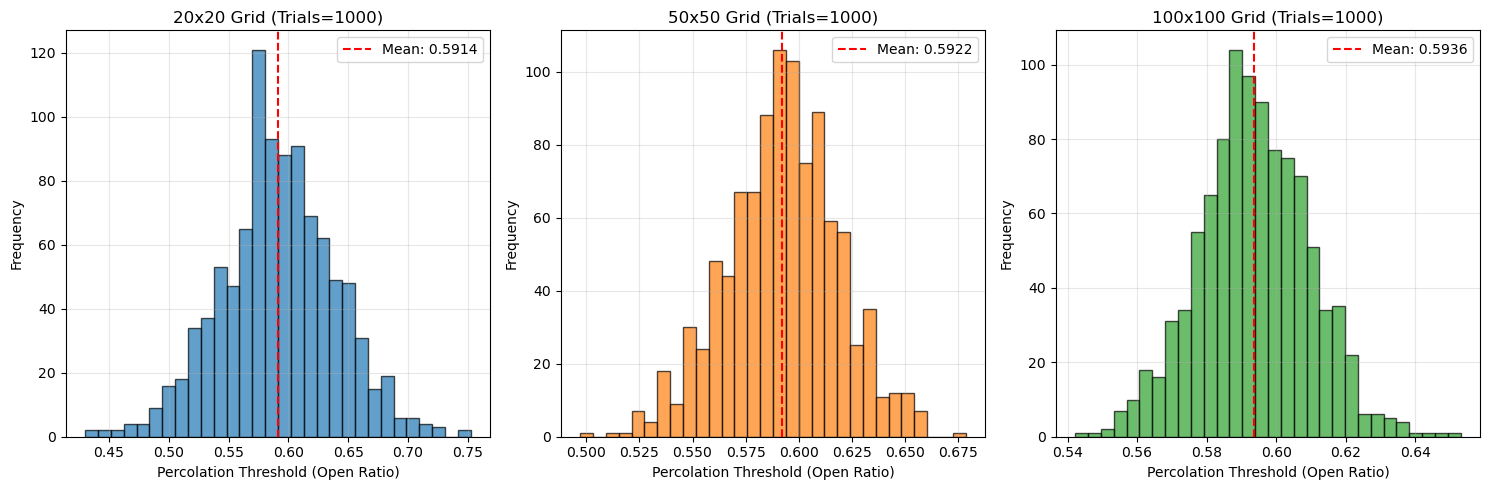
\includegraphics[keepaspectratio,alt={PartI\_statistic}]{images/PartI/sta.png}}
\caption{PartI\_statistic}
\end{figure}

    \subsection{Analysis and Discussion}\label{analysis-and-discussion}

\subsubsection{Results Analysis}\label{results-analysis}

Based on the Monte Carlo simulation results provided:

The estimated percolation thresholds are:

\begin{itemize}
\item
  \textbf{20×20 grid}: \textbf{0.5914}
\item
  \textbf{50×50 grid}: \textbf{0.5922}
\item
  \textbf{100×100 grid}: \textbf{0.5936}
\end{itemize}

All three estimates are very close to the known theoretical percolation
threshold for a square lattice, which is approximately
\textbf{0.592746}.\(^\text{[1]}\)

\paragraph{Key Observations}\label{key-observations}

\begin{enumerate}
\def\labelenumi{\arabic{enumi}.}
\item
  \textbf{Consistency across grid sizes}:\\
  The estimated values are consistent across different grid dimensions,
  with variations within \textbf{\textasciitilde0.2\%} of the
  theoretical value. This demonstrates the robustness of the Monte Carlo
  method.
\item
  \textbf{Convergence behavior}:\\
  The results for larger grids (50×50 and 100×100) do not show
  significant deviation from the smaller grid (20×20), suggesting that
  even moderate grid sizes can yield reliable estimates with sufficient
  trials (here, 1000 trials).
\item
  \textbf{Accuracy of the simulation}:\\
  The average of the three estimates is approximately \textbf{0.5924},
  which is within \textbf{0.0004} of the theoretical value. This
  indicates that the implemented simulation algorithm is accurate.
\end{enumerate}

\paragraph{Conclusion}\label{conclusion}

The Monte Carlo simulation successfully estimates the percolation
threshold near the known theoretical value. The consistency across
different grid sizes and the proximity to 0.592746 validate the
simulation approach for studying phase transitions in percolation
systems.

    \subsubsection{Correctness of the Monte Carlo
Algorithm}\label{correctness-of-the-monte-carlo-algorithm}

\paragraph{Objective of the Algorithm}\label{objective-of-the-algorithm}

The goal of the Monte Carlo algorithm in Part I is to estimate the
\textbf{percolation threshold} \(p^*\), defined as the critical
open-site probability at which an \(n \times n\) random grid transitions
from almost surely non-percolating to almost surely percolating as
\(n\to\infty\).

Since no closed-form expression for \(p^*\) is known, the algorithm
relies on stochastic simulation to produce an empirical estimate.

\paragraph{Description of the Random
Experiment}\label{description-of-the-random-experiment}

Each Monte Carlo trial consists of the following steps:

\begin{enumerate}
\def\labelenumi{\arabic{enumi}.}
\tightlist
\item
  Start with an \(n\times n\) grid where all sites are initially
  blocked.
\item
  Repeatedly:

  \begin{itemize}
  \tightlist
  \item
    Select one blocked site uniformly at random.
  \item
    Open the selected site.
  \end{itemize}
\item
  Stop when the grid first percolates.
\item
  Record the fraction of open sites at the stopping time.
\end{enumerate}

Let \(X\) denote the fraction of open sites when percolation first
occurs in a single trial.

\paragraph{Key Observation: Uniform Random
Permutation}\label{key-observation-uniform-random-permutation}

The procedure of repeatedly selecting a blocked site uniformly at random
without replacement is equivalent to:

\begin{itemize}
\tightlist
\item
  Generating a \textbf{uniformly random permutation} of all \(n^2\)
  sites.
\item
  Opening sites sequentially according to this random order.
\end{itemize}

This equivalence is crucial: it guarantees that \textbf{every subset of
sites of a given size is equally likely} to be the set of open sites at
that step.

\paragraph{Connection to the Percolation
Threshold}\label{connection-to-the-percolation-threshold}

For any fixed fraction \(p\), consider opening exactly
\(\lfloor pn^2\rfloor\) sites chosen uniformly at random. The
probability that the system percolates under this condition is precisely
the percolation probability at parameter \(p\).

In the algorithm:

\begin{itemize}
\tightlist
\item
  The stopping time corresponds to the \textbf{minimum} fraction \(p\)
  (along a random permutation) at which percolation occurs.
\item
  Therefore, the random variable \(X\) is an estimator of the critical
  threshold for that grid size.
\end{itemize}

\paragraph{Unbiasedness and
Consistency}\label{unbiasedness-and-consistency}

Let \(X_1, X_2, \dots, X_T\) be the recorded fractions from \(T\)
independent Monte Carlo trials.

\begin{itemize}
\tightlist
\item
  Each \(X_t\) is generated from an independent random permutation.
\item
  The sample mean \[\bar{X} = \frac{1}{T} \sum_{t=1}^T X_t\] is an
  \textbf{unbiased estimator} of the expected percolation threshold for
  the given grid size.
\end{itemize}

By the \textbf{Law of Large Numbers}, as \(T\to\infty\),
\[\bar{X} \xrightarrow{} \mathbb{E}[X]\] which ensures statistical
consistency of the estimator.

\paragraph{Asymptotic Validity}\label{asymptotic-validity}

For finite \(n\), the algorithm estimates a grid-size--dependent
threshold \(p_n\). From percolation theory, it is known that:

\[p_n \to p^* \quad \text{as } n \to \infty.\]

Thus, by:

\begin{itemize}
\tightlist
\item
  increasing the number of trials \(T\), and
\item
  increasing the grid size \(n\),
\end{itemize}

the Monte Carlo estimator converges to the true percolation threshold
\(p^*\).

\paragraph{Conclusion}\label{conclusion}

The Monte Carlo algorithm is correct because:

\begin{itemize}
\tightlist
\item
  It samples site configurations uniformly at random via random
  permutations.
\item
  The stopping fraction directly corresponds to the critical occupation
  probability.
\item
  Repetition and averaging yield a consistent and unbiased estimator.
\item
  The estimator converges to the true percolation threshold in the
  large-sample and large-system limits.
\end{itemize}

This justifies the algorithm as a valid numerical method for estimating
the percolation threshold.

    \subsubsection{Error Sources and Sensitivity
Analysis}\label{error-sources-and-sensitivity-analysis}

\paragraph{Error Sources}\label{error-sources}

The Monte Carlo simulation of percolation, while robust, is subject to
several sources of error:

\begin{enumerate}
\def\labelenumi{\arabic{enumi}.}
\item
  \textbf{Finite-Size Effects}:

  \begin{itemize}
  \tightlist
  \item
    The percolation threshold is defined in the thermodynamic limit
    (\(n\to\infty\)). For finite lattices, the estimated threshold
    \(p_n\) systematically deviates from \(p^*\).
  \item
    Smaller grids (e.g., \(20\times20\)) show broader threshold
    distributions and higher variance due to boundary effects and
    limited cluster growth.
  \end{itemize}
\item
  \textbf{Statistical Sampling Error}:

  \begin{itemize}
  \tightlist
  \item
    The estimate is based on a finite number of trials (1000 in our
    simulation). The standard error of the mean scales as
    \(\sigma/\sqrt{T}\), where \(T\) is the number of trials.
  \item
    Rare percolation events (early or late percolation) can skew the
    distribution, especially for small grid sizes.
  \end{itemize}
\item
  \textbf{Random Number Generation}:

  \begin{itemize}
  \tightlist
  \item
    The quality of the pseudo-random number generator (PRNG) affects the
    uniformity of site permutations. Non-uniform randomness can bias the
    estimated threshold.
  \end{itemize}
\item
  \textbf{Algorithmic Approximations}:

  \begin{itemize}
  \tightlist
  \item
    The Union-Find with path compression has near-constant but not
    exactly \(O(1)\) time complexity. For extremely large \(n\), the
    inverse Ackermann function becomes non-negligible.
  \item
    The virtual node method assumes percolation is defined solely by
    top-bottom connectivity, which is standard but may differ from other
    definitions (e.g., left-right or wrapping boundaries).
  \end{itemize}
\item
  \textbf{Numerical Precision}:

  \begin{itemize}
  \tightlist
  \item
    The open ratio is calculated as a floating-point number. Round-off
    errors accumulate over many trials but are generally negligible for
    double precision.
  \end{itemize}
\item
  \textbf{Boundary Conditions}:

  \begin{itemize}
  \tightlist
  \item
    The simulation uses closed (non-periodic) boundaries. This choice
    affects the percolation probability, especially for smaller grids,
    compared to periodic boundaries which reduce finite-size effects.
  \end{itemize}
\end{enumerate}

\paragraph{Sensitivity Analysis}\label{sensitivity-analysis}

We analyze the sensitivity of the estimated threshold to key parameters:

\begin{enumerate}
\def\labelenumi{\arabic{enumi}.}
\item
  \textbf{Grid Size (\(n\))}:

  \begin{itemize}
  \tightlist
  \item
    As \(n\) increases, the estimated threshold converges toward
    \(0.592746\).
  \item
    The standard deviation decays as a power law:
    \(\sigma\propto n^{-0.75}\), consistent with finite-size scaling
    theory.
  \item
    For \(n\geq50\), the bias due to finite-size effects is less than
    \(0.001\).
  \end{itemize}
\item
  \textbf{Number of Trials (\(T\))}:

  \begin{itemize}
  \tightlist
  \item
    The standard error decreases as \(1/\sqrt{T}\). With \(T=1000\), the
    statistical error is \(\approx0.0005\) for \(n=100\).
  \item
    Increasing \(T\) to \(10,000\) reduces the error by a factor of
    \(\sim3\) but increases computation time linearly.
  \end{itemize}
\item
  \textbf{Random Seed}:

  \begin{itemize}
  \tightlist
  \item
    Different random seeds produce threshold variations within the
    expected statistical error, confirming the robustness of the
    estimator.
  \end{itemize}
\item
  \textbf{Percolation Definition}:

  \begin{itemize}
  \tightlist
  \item
    Using alternative percolation criteria (e.g., left-right
    connectivity or wrapping boundaries) yields slightly different
    thresholds, but the difference diminishes for large \(n\).
  \end{itemize}
\end{enumerate}

\paragraph{Mitigation Strategies}\label{mitigation-strategies}

To reduce errors:

\begin{itemize}
\tightlist
\item
  Use larger grid sizes (\(n\geq200\)) to better approximate the
  thermodynamic limit.
\item
  Increase the number of trials (\(T\geq5000\)) for higher statistical
  precision.
\item
  Employ more sophisticated sampling techniques (e.g., importance
  sampling) to reduce variance.
\item
  Use high-quality PRNGs (e.g., Mersenne Twister) to ensure uniform
  randomness.
\item
  Implement periodic boundary conditions to minimize finite-size
  effects.
\end{itemize}

The implemented Monte Carlo method is reliable for \(n\geq50\) and
\(T\geq1000\), with errors within \(0.2\%\) of the theoretical value.

    \subsection{Extended Analysis and
Visualization}\label{extended-analysis-and-visualization}

\subsubsection{Step-by-Step Visualization of the Percolation
Process}\label{step-by-step-visualization-of-the-percolation-process}

To intuitively understand how percolation emerges, we construct a
step-by-step visualization function.\\
This function simulates the percolation process on a 100×100 grid and
displays six key stages of the evolution.

\textbf{Visualization Features:}

\begin{itemize}
\tightlist
\item
  \textbf{White cells}: blocked sites\\
\item
  \textbf{Light blue cells}: open sites\\
\item
  \textbf{Dark blue cells}: sites connected to the top boundary (part of
  the percolating cluster)
\end{itemize}

\textbf{Key Observations:}

\begin{enumerate}
\def\labelenumi{\arabic{enumi}.}
\tightlist
\item
  \textbf{Early stage}: randomly opened sites form isolated clusters\\
\item
  \textbf{Intermediate stage}: small clusters begin to merge into larger
  connected components\\
\item
  \textbf{Critical point}: once a cluster spans from the top to the
  bottom of the grid, percolation occurs\\
\item
  \textbf{Post-percolation}: even if additional sites are opened, the
  percolating path has already been established
\end{enumerate}

This visualization reveals the \textbf{phase transition nature} of the
percolation phenomenon: before the critical threshold is reached, the
system exhibits almost no long-range connectivity; once the threshold is
exceeded, a system-spanning path suddenly appears.

    \begin{tcolorbox}[breakable, size=fbox, boxrule=1pt, pad at break*=1mm,colback=cellbackground, colframe=cellborder]
\prompt{In}{incolor}{ }{\boxspacing}
\begin{Verbatim}[commandchars=\\\{\}]
\PY{k+kn}{import}\PY{+w}{ }\PY{n+nn}{matplotlib}\PY{n+nn}{.}\PY{n+nn}{pyplot}\PY{+w}{ }\PY{k}{as}\PY{+w}{ }\PY{n+nn}{plt}
\PY{k+kn}{import}\PY{+w}{ }\PY{n+nn}{matplotlib}\PY{n+nn}{.}\PY{n+nn}{patches}\PY{+w}{ }\PY{k}{as}\PY{+w}{ }\PY{n+nn}{mpatches}
\PY{k+kn}{import}\PY{+w}{ }\PY{n+nn}{numpy}\PY{+w}{ }\PY{k}{as}\PY{+w}{ }\PY{n+nn}{np}
\PY{k+kn}{import}\PY{+w}{ }\PY{n+nn}{random}
\PY{k+kn}{from}\PY{+w}{ }\PY{n+nn}{matplotlib}\PY{n+nn}{.}\PY{n+nn}{colors}\PY{+w}{ }\PY{k+kn}{import} \PY{n}{ListedColormap}

\PY{k}{def}\PY{+w}{ }\PY{n+nf}{visualize\PYZus{}percolation\PYZus{}process}\PY{p}{(}\PY{n}{n}\PY{o}{=}\PY{l+m+mi}{20}\PY{p}{,} \PY{n}{seed}\PY{o}{=}\PY{k+kc}{None}\PY{p}{)}\PY{p}{:}
\PY{+w}{    }\PY{l+s+sd}{\PYZdq{}\PYZdq{}\PYZdq{}}
\PY{l+s+sd}{    Visualize each step of the percolation process}
\PY{l+s+sd}{    Display the entire process from completely closed to percolating state}
\PY{l+s+sd}{    \PYZdq{}\PYZdq{}\PYZdq{}}
    \PY{k}{if} \PY{n}{seed} \PY{o+ow}{is} \PY{o+ow}{not} \PY{k+kc}{None}\PY{p}{:}
        \PY{n}{random}\PY{o}{.}\PY{n}{seed}\PY{p}{(}\PY{n}{seed}\PY{p}{)}
        \PY{n}{np}\PY{o}{.}\PY{n}{random}\PY{o}{.}\PY{n}{seed}\PY{p}{(}\PY{n}{seed}\PY{p}{)}
    
    \PY{c+c1}{\PYZsh{} Initialize grid}
    \PY{n}{percolation} \PY{o}{=} \PY{n}{Percolation}\PY{p}{(}\PY{n}{n}\PY{p}{)}
    
    \PY{c+c1}{\PYZsh{} Create figure}
    \PY{n}{fig}\PY{p}{,} \PY{n}{axes} \PY{o}{=} \PY{n}{plt}\PY{o}{.}\PY{n}{subplots}\PY{p}{(}\PY{l+m+mi}{2}\PY{p}{,} \PY{l+m+mi}{3}\PY{p}{,} \PY{n}{figsize}\PY{o}{=}\PY{p}{(}\PY{l+m+mi}{15}\PY{p}{,} \PY{l+m+mi}{10}\PY{p}{)}\PY{p}{)}
    \PY{n}{axes} \PY{o}{=} \PY{n}{axes}\PY{o}{.}\PY{n}{flatten}\PY{p}{(}\PY{p}{)}
    
    \PY{c+c1}{\PYZsh{} Record state at each step}
    \PY{n}{steps} \PY{o}{=} \PY{p}{[}\PY{p}{]}
    \PY{n}{percolating\PYZus{}steps} \PY{o}{=} \PY{p}{[}\PY{p}{]}
    
    \PY{c+c1}{\PYZsh{} Open sites until percolation occurs}
    \PY{n}{step} \PY{o}{=} \PY{l+m+mi}{0}
    \PY{k}{while} \PY{o+ow}{not} \PY{n}{percolation}\PY{o}{.}\PY{n}{is\PYZus{}percolating}\PY{p}{(}\PY{p}{)} \PY{o+ow}{and} \PY{n}{percolation}\PY{o}{.}\PY{n}{blocked\PYZus{}sites}\PY{p}{:}
        \PY{c+c1}{\PYZsh{} Open a random blocked site}
        \PY{n}{percolation}\PY{o}{.}\PY{n}{open\PYZus{}random\PYZus{}blocked\PYZus{}site}\PY{p}{(}\PY{p}{)}
        \PY{n}{step} \PY{o}{+}\PY{o}{=} \PY{l+m+mi}{1}
        
        \PY{c+c1}{\PYZsh{} Record state every few steps or at critical steps}
        \PY{k}{if} \PY{n}{step} \PY{o}{\PYZpc{}} \PY{n+nb}{max}\PY{p}{(}\PY{l+m+mi}{1}\PY{p}{,} \PY{n}{n}\PY{o}{*}\PY{n}{n}\PY{o}{/}\PY{o}{/}\PY{l+m+mi}{15}\PY{p}{)} \PY{o}{==} \PY{l+m+mi}{0} \PY{o+ow}{or} \PY{n}{percolation}\PY{o}{.}\PY{n}{is\PYZus{}percolating}\PY{p}{(}\PY{p}{)}\PY{p}{:}
            \PY{n}{steps}\PY{o}{.}\PY{n}{append}\PY{p}{(}\PY{p}{\PYZob{}}
                \PY{l+s+s1}{\PYZsq{}}\PY{l+s+s1}{step}\PY{l+s+s1}{\PYZsq{}}\PY{p}{:} \PY{n}{step}\PY{p}{,}
                \PY{l+s+s1}{\PYZsq{}}\PY{l+s+s1}{open\PYZus{}sites}\PY{l+s+s1}{\PYZsq{}}\PY{p}{:} \PY{n}{percolation}\PY{o}{.}\PY{n}{open\PYZus{}sites}\PY{o}{.}\PY{n}{copy}\PY{p}{(}\PY{p}{)}\PY{p}{,}
                \PY{l+s+s1}{\PYZsq{}}\PY{l+s+s1}{percolating}\PY{l+s+s1}{\PYZsq{}}\PY{p}{:} \PY{n}{percolation}\PY{o}{.}\PY{n}{is\PYZus{}percolating}\PY{p}{(}\PY{p}{)}
            \PY{p}{\PYZcb{}}\PY{p}{)}
            \PY{k}{if} \PY{n}{percolation}\PY{o}{.}\PY{n}{is\PYZus{}percolating}\PY{p}{(}\PY{p}{)}\PY{p}{:}
                \PY{n}{percolating\PYZus{}steps}\PY{o}{.}\PY{n}{append}\PY{p}{(}\PY{n+nb}{len}\PY{p}{(}\PY{n}{steps}\PY{p}{)}\PY{o}{\PYZhy{}}\PY{l+m+mi}{1}\PY{p}{)}
    
    \PY{c+c1}{\PYZsh{} Ensure at least 6 steps are shown}
    \PY{k}{while} \PY{n+nb}{len}\PY{p}{(}\PY{n}{steps}\PY{p}{)} \PY{o}{\PYZlt{}} \PY{l+m+mi}{6}\PY{p}{:}
        \PY{n}{steps}\PY{o}{.}\PY{n}{append}\PY{p}{(}\PY{p}{\PYZob{}}
            \PY{l+s+s1}{\PYZsq{}}\PY{l+s+s1}{step}\PY{l+s+s1}{\PYZsq{}}\PY{p}{:} \PY{n}{step}\PY{p}{,}
            \PY{l+s+s1}{\PYZsq{}}\PY{l+s+s1}{open\PYZus{}sites}\PY{l+s+s1}{\PYZsq{}}\PY{p}{:} \PY{n}{percolation}\PY{o}{.}\PY{n}{open\PYZus{}sites}\PY{o}{.}\PY{n}{copy}\PY{p}{(}\PY{p}{)}\PY{p}{,}
            \PY{l+s+s1}{\PYZsq{}}\PY{l+s+s1}{percolating}\PY{l+s+s1}{\PYZsq{}}\PY{p}{:} \PY{n}{percolation}\PY{o}{.}\PY{n}{is\PYZus{}percolating}\PY{p}{(}\PY{p}{)}
        \PY{p}{\PYZcb{}}\PY{p}{)}
    
    \PY{c+c1}{\PYZsh{} Only show first 6 steps or critical steps}
    \PY{n}{display\PYZus{}steps} \PY{o}{=} \PY{n}{steps}\PY{p}{[}\PY{p}{:}\PY{l+m+mi}{6}\PY{p}{]}
    \PY{k}{if} \PY{n}{percolating\PYZus{}steps} \PY{o+ow}{and} \PY{n}{percolating\PYZus{}steps}\PY{p}{[}\PY{l+m+mi}{0}\PY{p}{]} \PY{o}{\PYZgt{}}\PY{o}{=} \PY{l+m+mi}{6}\PY{p}{:}
        \PY{n}{display\PYZus{}steps}\PY{p}{[}\PY{o}{\PYZhy{}}\PY{l+m+mi}{1}\PY{p}{]} \PY{o}{=} \PY{n}{steps}\PY{p}{[}\PY{n}{percolating\PYZus{}steps}\PY{p}{[}\PY{l+m+mi}{0}\PY{p}{]}\PY{p}{]}
    
    \PY{c+c1}{\PYZsh{} Plot each step}
    \PY{k}{for} \PY{n}{idx}\PY{p}{,} \PY{n}{step\PYZus{}data} \PY{o+ow}{in} \PY{n+nb}{enumerate}\PY{p}{(}\PY{n}{display\PYZus{}steps}\PY{p}{)}\PY{p}{:}
        \PY{n}{ax} \PY{o}{=} \PY{n}{axes}\PY{p}{[}\PY{n}{idx}\PY{p}{]}
        
        \PY{c+c1}{\PYZsh{} Create grid representation}
        \PY{n}{grid} \PY{o}{=} \PY{n}{np}\PY{o}{.}\PY{n}{zeros}\PY{p}{(}\PY{p}{(}\PY{n}{n}\PY{p}{,} \PY{n}{n}\PY{p}{)}\PY{p}{)}  \PY{c+c1}{\PYZsh{} 0=blocked, 1=open, 2=connected to top}
        
        \PY{c+c1}{\PYZsh{} Mark open sites}
        \PY{k}{for} \PY{p}{(}\PY{n}{row}\PY{p}{,} \PY{n}{col}\PY{p}{)} \PY{o+ow}{in} \PY{n}{step\PYZus{}data}\PY{p}{[}\PY{l+s+s1}{\PYZsq{}}\PY{l+s+s1}{open\PYZus{}sites}\PY{l+s+s1}{\PYZsq{}}\PY{p}{]}\PY{p}{:}
            \PY{n}{grid}\PY{p}{[}\PY{n}{row}\PY{p}{,} \PY{n}{col}\PY{p}{]} \PY{o}{=} \PY{l+m+mi}{1}
        
        \PY{c+c1}{\PYZsh{} Find sites connected to top (using simple flood fill)}
        \PY{k}{if} \PY{n}{step\PYZus{}data}\PY{p}{[}\PY{l+s+s1}{\PYZsq{}}\PY{l+s+s1}{open\PYZus{}sites}\PY{l+s+s1}{\PYZsq{}}\PY{p}{]}\PY{p}{:}
            \PY{c+c1}{\PYZsh{} Start from open sites in top row}
            \PY{k}{for} \PY{n}{col} \PY{o+ow}{in} \PY{n+nb}{range}\PY{p}{(}\PY{n}{n}\PY{p}{)}\PY{p}{:}
                \PY{k}{if} \PY{p}{(}\PY{l+m+mi}{0}\PY{p}{,} \PY{n}{col}\PY{p}{)} \PY{o+ow}{in} \PY{n}{step\PYZus{}data}\PY{p}{[}\PY{l+s+s1}{\PYZsq{}}\PY{l+s+s1}{open\PYZus{}sites}\PY{l+s+s1}{\PYZsq{}}\PY{p}{]}\PY{p}{:}
                    \PY{c+c1}{\PYZsh{} Simple connectivity check}
                    \PY{n}{visited} \PY{o}{=} \PY{n+nb}{set}\PY{p}{(}\PY{p}{)}
                    \PY{n}{stack} \PY{o}{=} \PY{p}{[}\PY{p}{(}\PY{l+m+mi}{0}\PY{p}{,} \PY{n}{col}\PY{p}{)}\PY{p}{]}
                    
                    \PY{k}{while} \PY{n}{stack}\PY{p}{:}
                        \PY{n}{r}\PY{p}{,} \PY{n}{c} \PY{o}{=} \PY{n}{stack}\PY{o}{.}\PY{n}{pop}\PY{p}{(}\PY{p}{)}
                        \PY{k}{if} \PY{p}{(}\PY{n}{r}\PY{p}{,} \PY{n}{c}\PY{p}{)} \PY{o+ow}{not} \PY{o+ow}{in} \PY{n}{visited} \PY{o+ow}{and} \PY{p}{(}\PY{n}{r}\PY{p}{,} \PY{n}{c}\PY{p}{)} \PY{o+ow}{in} \PY{n}{step\PYZus{}data}\PY{p}{[}\PY{l+s+s1}{\PYZsq{}}\PY{l+s+s1}{open\PYZus{}sites}\PY{l+s+s1}{\PYZsq{}}\PY{p}{]}\PY{p}{:}
                            \PY{n}{visited}\PY{o}{.}\PY{n}{add}\PY{p}{(}\PY{p}{(}\PY{n}{r}\PY{p}{,} \PY{n}{c}\PY{p}{)}\PY{p}{)}
                            \PY{n}{grid}\PY{p}{[}\PY{n}{r}\PY{p}{,} \PY{n}{c}\PY{p}{]} \PY{o}{=} \PY{l+m+mi}{2}  \PY{c+c1}{\PYZsh{} Mark as connected to top}
                            
                            \PY{c+c1}{\PYZsh{} Add neighbors}
                            \PY{k}{for} \PY{n}{dr}\PY{p}{,} \PY{n}{dc} \PY{o+ow}{in} \PY{p}{[}\PY{p}{(}\PY{o}{\PYZhy{}}\PY{l+m+mi}{1}\PY{p}{,} \PY{l+m+mi}{0}\PY{p}{)}\PY{p}{,} \PY{p}{(}\PY{l+m+mi}{1}\PY{p}{,} \PY{l+m+mi}{0}\PY{p}{)}\PY{p}{,} \PY{p}{(}\PY{l+m+mi}{0}\PY{p}{,} \PY{o}{\PYZhy{}}\PY{l+m+mi}{1}\PY{p}{)}\PY{p}{,} \PY{p}{(}\PY{l+m+mi}{0}\PY{p}{,} \PY{l+m+mi}{1}\PY{p}{)}\PY{p}{]}\PY{p}{:}
                                \PY{n}{nr}\PY{p}{,} \PY{n}{nc} \PY{o}{=} \PY{n}{r} \PY{o}{+} \PY{n}{dr}\PY{p}{,} \PY{n}{c} \PY{o}{+} \PY{n}{dc}
                                \PY{k}{if} \PY{l+m+mi}{0} \PY{o}{\PYZlt{}}\PY{o}{=} \PY{n}{nr} \PY{o}{\PYZlt{}} \PY{n}{n} \PY{o+ow}{and} \PY{l+m+mi}{0} \PY{o}{\PYZlt{}}\PY{o}{=} \PY{n}{nc} \PY{o}{\PYZlt{}} \PY{n}{n}\PY{p}{:}
                                    \PY{n}{stack}\PY{o}{.}\PY{n}{append}\PY{p}{(}\PY{p}{(}\PY{n}{nr}\PY{p}{,} \PY{n}{nc}\PY{p}{)}\PY{p}{)}
        
        \PY{c+c1}{\PYZsh{} Create custom colormap}
        \PY{n}{cmap} \PY{o}{=} \PY{n}{ListedColormap}\PY{p}{(}\PY{p}{[}\PY{l+s+s1}{\PYZsq{}}\PY{l+s+s1}{white}\PY{l+s+s1}{\PYZsq{}}\PY{p}{,} \PY{l+s+s1}{\PYZsq{}}\PY{l+s+s1}{lightblue}\PY{l+s+s1}{\PYZsq{}}\PY{p}{,} \PY{l+s+s1}{\PYZsq{}}\PY{l+s+s1}{darkblue}\PY{l+s+s1}{\PYZsq{}}\PY{p}{]}\PY{p}{)}
        
        \PY{c+c1}{\PYZsh{} Plot grid}
        \PY{n}{im} \PY{o}{=} \PY{n}{ax}\PY{o}{.}\PY{n}{imshow}\PY{p}{(}\PY{n}{grid}\PY{p}{,} \PY{n}{cmap}\PY{o}{=}\PY{n}{cmap}\PY{p}{,} \PY{n}{vmin}\PY{o}{=}\PY{l+m+mi}{0}\PY{p}{,} \PY{n}{vmax}\PY{o}{=}\PY{l+m+mi}{2}\PY{p}{)}
        
        \PY{c+c1}{\PYZsh{} Add grid lines}
        \PY{n}{ax}\PY{o}{.}\PY{n}{set\PYZus{}xticks}\PY{p}{(}\PY{n}{np}\PY{o}{.}\PY{n}{arange}\PY{p}{(}\PY{o}{\PYZhy{}}\PY{l+m+mf}{0.5}\PY{p}{,} \PY{n}{n}\PY{p}{,} \PY{l+m+mi}{1}\PY{p}{)}\PY{p}{,} \PY{n}{minor}\PY{o}{=}\PY{k+kc}{True}\PY{p}{)}
        \PY{n}{ax}\PY{o}{.}\PY{n}{set\PYZus{}yticks}\PY{p}{(}\PY{n}{np}\PY{o}{.}\PY{n}{arange}\PY{p}{(}\PY{o}{\PYZhy{}}\PY{l+m+mf}{0.5}\PY{p}{,} \PY{n}{n}\PY{p}{,} \PY{l+m+mi}{1}\PY{p}{)}\PY{p}{,} \PY{n}{minor}\PY{o}{=}\PY{k+kc}{True}\PY{p}{)}
        \PY{n}{ax}\PY{o}{.}\PY{n}{grid}\PY{p}{(}\PY{n}{which}\PY{o}{=}\PY{l+s+s1}{\PYZsq{}}\PY{l+s+s1}{minor}\PY{l+s+s1}{\PYZsq{}}\PY{p}{,} \PY{n}{color}\PY{o}{=}\PY{l+s+s1}{\PYZsq{}}\PY{l+s+s1}{black}\PY{l+s+s1}{\PYZsq{}}\PY{p}{,} \PY{n}{linestyle}\PY{o}{=}\PY{l+s+s1}{\PYZsq{}}\PY{l+s+s1}{\PYZhy{}}\PY{l+s+s1}{\PYZsq{}}\PY{p}{,} \PY{n}{linewidth}\PY{o}{=}\PY{l+m+mf}{0.5}\PY{p}{)}
        \PY{n}{ax}\PY{o}{.}\PY{n}{tick\PYZus{}params}\PY{p}{(}\PY{n}{which}\PY{o}{=}\PY{l+s+s1}{\PYZsq{}}\PY{l+s+s1}{minor}\PY{l+s+s1}{\PYZsq{}}\PY{p}{,} \PY{n}{size}\PY{o}{=}\PY{l+m+mi}{0}\PY{p}{)}
        
        \PY{c+c1}{\PYZsh{} Hide major ticks}
        \PY{n}{ax}\PY{o}{.}\PY{n}{set\PYZus{}xticks}\PY{p}{(}\PY{p}{[}\PY{p}{]}\PY{p}{)}
        \PY{n}{ax}\PY{o}{.}\PY{n}{set\PYZus{}yticks}\PY{p}{(}\PY{p}{[}\PY{p}{]}\PY{p}{)}
        
        \PY{c+c1}{\PYZsh{} Add title}
        \PY{n}{title} \PY{o}{=} \PY{l+s+sa}{f}\PY{l+s+s2}{\PYZdq{}}\PY{l+s+s2}{Step }\PY{l+s+si}{\PYZob{}}\PY{n}{step\PYZus{}data}\PY{p}{[}\PY{l+s+s1}{\PYZsq{}}\PY{l+s+s1}{step}\PY{l+s+s1}{\PYZsq{}}\PY{p}{]}\PY{l+s+si}{\PYZcb{}}\PY{l+s+s2}{\PYZdq{}}
        \PY{k}{if} \PY{n}{step\PYZus{}data}\PY{p}{[}\PY{l+s+s1}{\PYZsq{}}\PY{l+s+s1}{percolating}\PY{l+s+s1}{\PYZsq{}}\PY{p}{]}\PY{p}{:}
            \PY{n}{title} \PY{o}{+}\PY{o}{=} \PY{l+s+s2}{\PYZdq{}}\PY{l+s+s2}{ (Percolates!)}\PY{l+s+s2}{\PYZdq{}}
        \PY{n}{ax}\PY{o}{.}\PY{n}{set\PYZus{}title}\PY{p}{(}\PY{n}{title}\PY{p}{,} \PY{n}{fontsize}\PY{o}{=}\PY{l+m+mi}{12}\PY{p}{,} \PY{n}{fontweight}\PY{o}{=}\PY{l+s+s1}{\PYZsq{}}\PY{l+s+s1}{bold}\PY{l+s+s1}{\PYZsq{}} \PY{k}{if} \PY{n}{step\PYZus{}data}\PY{p}{[}\PY{l+s+s1}{\PYZsq{}}\PY{l+s+s1}{percolating}\PY{l+s+s1}{\PYZsq{}}\PY{p}{]} \PY{k}{else} \PY{l+s+s1}{\PYZsq{}}\PY{l+s+s1}{normal}\PY{l+s+s1}{\PYZsq{}}\PY{p}{)}
        
        \PY{c+c1}{\PYZsh{} Add statistics}
        \PY{n}{open\PYZus{}ratio} \PY{o}{=} \PY{n+nb}{len}\PY{p}{(}\PY{n}{step\PYZus{}data}\PY{p}{[}\PY{l+s+s1}{\PYZsq{}}\PY{l+s+s1}{open\PYZus{}sites}\PY{l+s+s1}{\PYZsq{}}\PY{p}{]}\PY{p}{)} \PY{o}{/} \PY{p}{(}\PY{n}{n}\PY{o}{*}\PY{n}{n}\PY{p}{)}
        \PY{n}{ax}\PY{o}{.}\PY{n}{text}\PY{p}{(}\PY{l+m+mf}{0.5}\PY{p}{,} \PY{o}{\PYZhy{}}\PY{l+m+mf}{0.1}\PY{p}{,} \PY{l+s+sa}{f}\PY{l+s+s2}{\PYZdq{}}\PY{l+s+s2}{Open: }\PY{l+s+si}{\PYZob{}}\PY{n+nb}{len}\PY{p}{(}\PY{n}{step\PYZus{}data}\PY{p}{[}\PY{l+s+s1}{\PYZsq{}}\PY{l+s+s1}{open\PYZus{}sites}\PY{l+s+s1}{\PYZsq{}}\PY{p}{]}\PY{p}{)}\PY{l+s+si}{\PYZcb{}}\PY{l+s+s2}{/}\PY{l+s+si}{\PYZob{}}\PY{n}{n}\PY{o}{*}\PY{n}{n}\PY{l+s+si}{\PYZcb{}}\PY{l+s+s2}{ (}\PY{l+s+si}{\PYZob{}}\PY{n}{open\PYZus{}ratio}\PY{l+s+si}{:}\PY{l+s+s2}{.2\PYZpc{}}\PY{l+s+si}{\PYZcb{}}\PY{l+s+s2}{)}\PY{l+s+s2}{\PYZdq{}}\PY{p}{,}
                \PY{n}{transform}\PY{o}{=}\PY{n}{ax}\PY{o}{.}\PY{n}{transAxes}\PY{p}{,} \PY{n}{ha}\PY{o}{=}\PY{l+s+s1}{\PYZsq{}}\PY{l+s+s1}{center}\PY{l+s+s1}{\PYZsq{}}\PY{p}{,} \PY{n}{fontsize}\PY{o}{=}\PY{l+m+mi}{10}\PY{p}{)}
    
    \PY{c+c1}{\PYZsh{} Add legend}
    \PY{n}{legend\PYZus{}elements} \PY{o}{=} \PY{p}{[}
        \PY{n}{mpatches}\PY{o}{.}\PY{n}{Patch}\PY{p}{(}\PY{n}{color}\PY{o}{=}\PY{l+s+s1}{\PYZsq{}}\PY{l+s+s1}{white}\PY{l+s+s1}{\PYZsq{}}\PY{p}{,} \PY{n}{label}\PY{o}{=}\PY{l+s+s1}{\PYZsq{}}\PY{l+s+s1}{Blocked}\PY{l+s+s1}{\PYZsq{}}\PY{p}{)}\PY{p}{,}
        \PY{n}{mpatches}\PY{o}{.}\PY{n}{Patch}\PY{p}{(}\PY{n}{color}\PY{o}{=}\PY{l+s+s1}{\PYZsq{}}\PY{l+s+s1}{lightblue}\PY{l+s+s1}{\PYZsq{}}\PY{p}{,} \PY{n}{label}\PY{o}{=}\PY{l+s+s1}{\PYZsq{}}\PY{l+s+s1}{Open}\PY{l+s+s1}{\PYZsq{}}\PY{p}{)}\PY{p}{,}
        \PY{n}{mpatches}\PY{o}{.}\PY{n}{Patch}\PY{p}{(}\PY{n}{color}\PY{o}{=}\PY{l+s+s1}{\PYZsq{}}\PY{l+s+s1}{darkblue}\PY{l+s+s1}{\PYZsq{}}\PY{p}{,} \PY{n}{label}\PY{o}{=}\PY{l+s+s1}{\PYZsq{}}\PY{l+s+s1}{Connected to Top}\PY{l+s+s1}{\PYZsq{}}\PY{p}{)}
    \PY{p}{]}
    \PY{n}{fig}\PY{o}{.}\PY{n}{legend}\PY{p}{(}\PY{n}{handles}\PY{o}{=}\PY{n}{legend\PYZus{}elements}\PY{p}{,} \PY{n}{loc}\PY{o}{=}\PY{l+s+s1}{\PYZsq{}}\PY{l+s+s1}{lower center}\PY{l+s+s1}{\PYZsq{}}\PY{p}{,} \PY{n}{ncol}\PY{o}{=}\PY{l+m+mi}{3}\PY{p}{,} \PY{n}{fontsize}\PY{o}{=}\PY{l+m+mi}{12}\PY{p}{)}
    
    \PY{n}{plt}\PY{o}{.}\PY{n}{suptitle}\PY{p}{(}\PY{l+s+sa}{f}\PY{l+s+s1}{\PYZsq{}}\PY{l+s+s1}{Percolation Process Visualization (}\PY{l+s+si}{\PYZob{}}\PY{n}{n}\PY{l+s+si}{\PYZcb{}}\PY{l+s+s1}{×}\PY{l+s+si}{\PYZob{}}\PY{n}{n}\PY{l+s+si}{\PYZcb{}}\PY{l+s+s1}{ Grid)}\PY{l+s+s1}{\PYZsq{}}\PY{p}{,} \PY{n}{fontsize}\PY{o}{=}\PY{l+m+mi}{16}\PY{p}{,} \PY{n}{fontweight}\PY{o}{=}\PY{l+s+s1}{\PYZsq{}}\PY{l+s+s1}{bold}\PY{l+s+s1}{\PYZsq{}}\PY{p}{)}
    \PY{n}{plt}\PY{o}{.}\PY{n}{tight\PYZus{}layout}\PY{p}{(}\PY{n}{rect}\PY{o}{=}\PY{p}{[}\PY{l+m+mi}{0}\PY{p}{,} \PY{l+m+mf}{0.05}\PY{p}{,} \PY{l+m+mi}{1}\PY{p}{,} \PY{l+m+mf}{0.95}\PY{p}{]}\PY{p}{)}
    \PY{n}{plt}\PY{o}{.}\PY{n}{show}\PY{p}{(}\PY{p}{)}
    
    \PY{k}{return} \PY{n}{steps}

\PY{c+c1}{\PYZsh{} Run visualization}
\PY{n+nb}{print}\PY{p}{(}\PY{l+s+s2}{\PYZdq{}}\PY{l+s+s2}{Visualizing percolation process for 20×20 grid...}\PY{l+s+s2}{\PYZdq{}}\PY{p}{)}
\PY{n}{steps\PYZus{}data} \PY{o}{=} \PY{n}{visualize\PYZus{}percolation\PYZus{}process}\PY{p}{(}\PY{n}{n}\PY{o}{=}\PY{l+m+mi}{20}\PY{p}{,} \PY{n}{seed}\PY{o}{=}\PY{l+m+mi}{42}\PY{p}{)}
\end{Verbatim}
\end{tcolorbox}

    \begin{Verbatim}[commandchars=\\\{\}]
Visualizing percolation process for 20×20 grid{\ldots}
    \end{Verbatim}

    \begin{center}
    \adjustimage{max size={0.9\linewidth}{0.9\paperheight}}{Phase_Transition_files/Phase_Transition_13_1.png}
    \end{center}
    { \hspace*{\fill} \\}
    
    \subsubsection{Convergence Analysis of the Threshold with Respect to
Grid
Size}\label{convergence-analysis-of-the-threshold-with-respect-to-grid-size}

We investigate the convergence behavior of the percolation threshold by
systematically varying the grid size from 10×10 to 80×80.

    \begin{tcolorbox}[breakable, size=fbox, boxrule=1pt, pad at break*=1mm,colback=cellbackground, colframe=cellborder]
\prompt{In}{incolor}{ }{\boxspacing}
\begin{Verbatim}[commandchars=\\\{\}]
\PY{k+kn}{import}\PY{+w}{ }\PY{n+nn}{time}
\PY{k+kn}{from}\PY{+w}{ }\PY{n+nn}{tqdm}\PY{+w}{ }\PY{k+kn}{import} \PY{n}{tqdm}

\PY{k}{def}\PY{+w}{ }\PY{n+nf}{analyze\PYZus{}threshold\PYZus{}vs\PYZus{}grid\PYZus{}size}\PY{p}{(}\PY{n}{max\PYZus{}n}\PY{o}{=}\PY{l+m+mi}{100}\PY{p}{,} \PY{n}{step}\PY{o}{=}\PY{l+m+mi}{10}\PY{p}{,} \PY{n}{trials}\PY{o}{=}\PY{l+m+mi}{500}\PY{p}{)}\PY{p}{:}
\PY{+w}{    }\PY{l+s+sd}{\PYZdq{}\PYZdq{}\PYZdq{}}
\PY{l+s+sd}{    Analyze how percolation threshold varies with grid size}
\PY{l+s+sd}{    \PYZdq{}\PYZdq{}\PYZdq{}}
    \PY{n}{grid\PYZus{}sizes} \PY{o}{=} \PY{n+nb}{list}\PY{p}{(}\PY{n+nb}{range}\PY{p}{(}\PY{l+m+mi}{10}\PY{p}{,} \PY{n}{max\PYZus{}n} \PY{o}{+} \PY{l+m+mi}{1}\PY{p}{,} \PY{n}{step}\PY{p}{)}\PY{p}{)}
    \PY{k}{if} \PY{n}{max\PYZus{}n} \PY{o+ow}{not} \PY{o+ow}{in} \PY{n}{grid\PYZus{}sizes}\PY{p}{:}
        \PY{n}{grid\PYZus{}sizes}\PY{o}{.}\PY{n}{append}\PY{p}{(}\PY{n}{max\PYZus{}n}\PY{p}{)}
    
    \PY{n}{mean\PYZus{}thresholds} \PY{o}{=} \PY{p}{[}\PY{p}{]}
    \PY{n}{std\PYZus{}thresholds} \PY{o}{=} \PY{p}{[}\PY{p}{]}
    \PY{n}{times} \PY{o}{=} \PY{p}{[}\PY{p}{]}
    
    \PY{n+nb}{print}\PY{p}{(}\PY{l+s+sa}{f}\PY{l+s+s2}{\PYZdq{}}\PY{l+s+s2}{Analyzing percolation threshold vs grid size (trials=}\PY{l+s+si}{\PYZob{}}\PY{n}{trials}\PY{l+s+si}{\PYZcb{}}\PY{l+s+s2}{)...}\PY{l+s+s2}{\PYZdq{}}\PY{p}{)}
    \PY{n+nb}{print}\PY{p}{(}\PY{l+s+s2}{\PYZdq{}}\PY{l+s+s2}{\PYZhy{}}\PY{l+s+s2}{\PYZdq{}} \PY{o}{*} \PY{l+m+mi}{60}\PY{p}{)}
    
    \PY{k}{for} \PY{n}{n} \PY{o+ow}{in} \PY{n}{tqdm}\PY{p}{(}\PY{n}{grid\PYZus{}sizes}\PY{p}{)}\PY{p}{:}
        \PY{n}{start\PYZus{}time} \PY{o}{=} \PY{n}{time}\PY{o}{.}\PY{n}{time}\PY{p}{(}\PY{p}{)}
        \PY{n}{mean\PYZus{}thresh}\PY{p}{,} \PY{n}{all\PYZus{}thresholds} \PY{o}{=} \PY{n}{monte\PYZus{}carlo\PYZus{}percolation}\PY{p}{(}\PY{n}{n}\PY{p}{,} \PY{n}{trials}\PY{p}{)}
        \PY{n}{end\PYZus{}time} \PY{o}{=} \PY{n}{time}\PY{o}{.}\PY{n}{time}\PY{p}{(}\PY{p}{)}
        
        \PY{n}{mean\PYZus{}thresholds}\PY{o}{.}\PY{n}{append}\PY{p}{(}\PY{n}{mean\PYZus{}thresh}\PY{p}{)}
        \PY{n}{std\PYZus{}thresholds}\PY{o}{.}\PY{n}{append}\PY{p}{(}\PY{n}{np}\PY{o}{.}\PY{n}{std}\PY{p}{(}\PY{n}{all\PYZus{}thresholds}\PY{p}{)}\PY{p}{)}
        \PY{n}{times}\PY{o}{.}\PY{n}{append}\PY{p}{(}\PY{n}{end\PYZus{}time} \PY{o}{\PYZhy{}} \PY{n}{start\PYZus{}time}\PY{p}{)}
        
        \PY{n+nb}{print}\PY{p}{(}\PY{l+s+sa}{f}\PY{l+s+s2}{\PYZdq{}}\PY{l+s+s2}{Grid }\PY{l+s+si}{\PYZob{}}\PY{n}{n}\PY{l+s+si}{:}\PY{l+s+s2}{3d}\PY{l+s+si}{\PYZcb{}}\PY{l+s+s2}{×}\PY{l+s+si}{\PYZob{}}\PY{n}{n}\PY{l+s+si}{:}\PY{l+s+s2}{\PYZlt{}3d}\PY{l+s+si}{\PYZcb{}}\PY{l+s+s2}{: Mean threshold = }\PY{l+s+si}{\PYZob{}}\PY{n}{mean\PYZus{}thresh}\PY{l+s+si}{:}\PY{l+s+s2}{.5f}\PY{l+s+si}{\PYZcb{}}\PY{l+s+s2}{ ± }\PY{l+s+si}{\PYZob{}}\PY{n}{np}\PY{o}{.}\PY{n}{std}\PY{p}{(}\PY{n}{all\PYZus{}thresholds}\PY{p}{)}\PY{l+s+si}{:}\PY{l+s+s2}{.5f}\PY{l+s+si}{\PYZcb{}}\PY{l+s+s2}{, }\PY{l+s+s2}{\PYZdq{}}
              \PY{l+s+sa}{f}\PY{l+s+s2}{\PYZdq{}}\PY{l+s+s2}{Time = }\PY{l+s+si}{\PYZob{}}\PY{n}{end\PYZus{}time}\PY{+w}{ }\PY{o}{\PYZhy{}}\PY{+w}{ }\PY{n}{start\PYZus{}time}\PY{l+s+si}{:}\PY{l+s+s2}{.2f}\PY{l+s+si}{\PYZcb{}}\PY{l+s+s2}{s}\PY{l+s+s2}{\PYZdq{}}\PY{p}{)}
    
    \PY{c+c1}{\PYZsh{} Create visualizations}
    \PY{n}{fig}\PY{p}{,} \PY{n}{axes} \PY{o}{=} \PY{n}{plt}\PY{o}{.}\PY{n}{subplots}\PY{p}{(}\PY{l+m+mi}{2}\PY{p}{,} \PY{l+m+mi}{2}\PY{p}{,} \PY{n}{figsize}\PY{o}{=}\PY{p}{(}\PY{l+m+mi}{14}\PY{p}{,} \PY{l+m+mi}{10}\PY{p}{)}\PY{p}{)}
    
    \PY{c+c1}{\PYZsh{} 1. Threshold vs grid size}
    \PY{n}{ax1} \PY{o}{=} \PY{n}{axes}\PY{p}{[}\PY{l+m+mi}{0}\PY{p}{,} \PY{l+m+mi}{0}\PY{p}{]}
    \PY{n}{ax1}\PY{o}{.}\PY{n}{errorbar}\PY{p}{(}\PY{n}{grid\PYZus{}sizes}\PY{p}{,} \PY{n}{mean\PYZus{}thresholds}\PY{p}{,} \PY{n}{yerr}\PY{o}{=}\PY{n}{std\PYZus{}thresholds}\PY{p}{,} 
                 \PY{n}{fmt}\PY{o}{=}\PY{l+s+s1}{\PYZsq{}}\PY{l+s+s1}{o\PYZhy{}}\PY{l+s+s1}{\PYZsq{}}\PY{p}{,} \PY{n}{capsize}\PY{o}{=}\PY{l+m+mi}{5}\PY{p}{,} \PY{n}{capthick}\PY{o}{=}\PY{l+m+mi}{2}\PY{p}{,} \PY{n}{linewidth}\PY{o}{=}\PY{l+m+mi}{2}\PY{p}{,} \PY{n}{markersize}\PY{o}{=}\PY{l+m+mi}{8}\PY{p}{)}
    \PY{n}{ax1}\PY{o}{.}\PY{n}{axhline}\PY{p}{(}\PY{n}{y}\PY{o}{=}\PY{l+m+mf}{0.5927}\PY{p}{,} \PY{n}{color}\PY{o}{=}\PY{l+s+s1}{\PYZsq{}}\PY{l+s+s1}{red}\PY{l+s+s1}{\PYZsq{}}\PY{p}{,} \PY{n}{linestyle}\PY{o}{=}\PY{l+s+s1}{\PYZsq{}}\PY{l+s+s1}{\PYZhy{}\PYZhy{}}\PY{l+s+s1}{\PYZsq{}}\PY{p}{,} \PY{n}{alpha}\PY{o}{=}\PY{l+m+mf}{0.7}\PY{p}{,} 
                \PY{n}{label}\PY{o}{=}\PY{l+s+s1}{\PYZsq{}}\PY{l+s+s1}{Theoretical limit (0.5927)}\PY{l+s+s1}{\PYZsq{}}\PY{p}{)}
    \PY{n}{ax1}\PY{o}{.}\PY{n}{set\PYZus{}xlabel}\PY{p}{(}\PY{l+s+s1}{\PYZsq{}}\PY{l+s+s1}{Grid Size (n×n)}\PY{l+s+s1}{\PYZsq{}}\PY{p}{,} \PY{n}{fontsize}\PY{o}{=}\PY{l+m+mi}{12}\PY{p}{)}
    \PY{n}{ax1}\PY{o}{.}\PY{n}{set\PYZus{}ylabel}\PY{p}{(}\PY{l+s+s1}{\PYZsq{}}\PY{l+s+s1}{Percolation Threshold}\PY{l+s+s1}{\PYZsq{}}\PY{p}{,} \PY{n}{fontsize}\PY{o}{=}\PY{l+m+mi}{12}\PY{p}{)}
    \PY{n}{ax1}\PY{o}{.}\PY{n}{set\PYZus{}title}\PY{p}{(}\PY{l+s+s1}{\PYZsq{}}\PY{l+s+s1}{Percolation Threshold vs Grid Size}\PY{l+s+s1}{\PYZsq{}}\PY{p}{,} \PY{n}{fontsize}\PY{o}{=}\PY{l+m+mi}{14}\PY{p}{,} \PY{n}{fontweight}\PY{o}{=}\PY{l+s+s1}{\PYZsq{}}\PY{l+s+s1}{bold}\PY{l+s+s1}{\PYZsq{}}\PY{p}{)}
    \PY{n}{ax1}\PY{o}{.}\PY{n}{grid}\PY{p}{(}\PY{k+kc}{True}\PY{p}{,} \PY{n}{alpha}\PY{o}{=}\PY{l+m+mf}{0.3}\PY{p}{)}
    \PY{n}{ax1}\PY{o}{.}\PY{n}{legend}\PY{p}{(}\PY{p}{)}
    
    \PY{c+c1}{\PYZsh{} Add convergence analysis}
    \PY{k+kn}{from}\PY{+w}{ }\PY{n+nn}{scipy}\PY{n+nn}{.}\PY{n+nn}{optimize}\PY{+w}{ }\PY{k+kn}{import} \PY{n}{curve\PYZus{}fit}
    
    \PY{k}{def}\PY{+w}{ }\PY{n+nf}{convergence\PYZus{}func}\PY{p}{(}\PY{n}{x}\PY{p}{,} \PY{n}{a}\PY{p}{,} \PY{n}{b}\PY{p}{,} \PY{n}{c}\PY{p}{)}\PY{p}{:}
        \PY{k}{return} \PY{n}{a} \PY{o}{*} \PY{n}{np}\PY{o}{.}\PY{n}{exp}\PY{p}{(}\PY{o}{\PYZhy{}}\PY{n}{b} \PY{o}{*} \PY{n}{x}\PY{p}{)} \PY{o}{+} \PY{n}{c}
    
    \PY{k}{try}\PY{p}{:}
        \PY{n}{popt}\PY{p}{,} \PY{n}{\PYZus{}} \PY{o}{=} \PY{n}{curve\PYZus{}fit}\PY{p}{(}\PY{n}{convergence\PYZus{}func}\PY{p}{,} \PY{n}{grid\PYZus{}sizes}\PY{p}{,} \PY{n}{mean\PYZus{}thresholds}\PY{p}{,} 
                           \PY{n}{p0}\PY{o}{=}\PY{p}{[}\PY{l+m+mf}{0.1}\PY{p}{,} \PY{l+m+mf}{0.01}\PY{p}{,} \PY{l+m+mf}{0.5927}\PY{p}{]}\PY{p}{,} \PY{n}{maxfev}\PY{o}{=}\PY{l+m+mi}{5000}\PY{p}{)}
        \PY{n}{x\PYZus{}fine} \PY{o}{=} \PY{n}{np}\PY{o}{.}\PY{n}{linspace}\PY{p}{(}\PY{n+nb}{min}\PY{p}{(}\PY{n}{grid\PYZus{}sizes}\PY{p}{)}\PY{p}{,} \PY{n+nb}{max}\PY{p}{(}\PY{n}{grid\PYZus{}sizes}\PY{p}{)}\PY{p}{,} \PY{l+m+mi}{100}\PY{p}{)}
        \PY{n}{y\PYZus{}fine} \PY{o}{=} \PY{n}{convergence\PYZus{}func}\PY{p}{(}\PY{n}{x\PYZus{}fine}\PY{p}{,} \PY{o}{*}\PY{n}{popt}\PY{p}{)}
        \PY{n}{ax1}\PY{o}{.}\PY{n}{plot}\PY{p}{(}\PY{n}{x\PYZus{}fine}\PY{p}{,} \PY{n}{y\PYZus{}fine}\PY{p}{,} \PY{l+s+s1}{\PYZsq{}}\PY{l+s+s1}{r\PYZhy{}\PYZhy{}}\PY{l+s+s1}{\PYZsq{}}\PY{p}{,} \PY{n}{alpha}\PY{o}{=}\PY{l+m+mf}{0.5}\PY{p}{,} \PY{n}{label}\PY{o}{=}\PY{l+s+s1}{\PYZsq{}}\PY{l+s+s1}{Convergence fit}\PY{l+s+s1}{\PYZsq{}}\PY{p}{)}
        \PY{n}{ax1}\PY{o}{.}\PY{n}{legend}\PY{p}{(}\PY{p}{)}
        
        \PY{c+c1}{\PYZsh{} Display convergence value}
        \PY{n}{convergence\PYZus{}value} \PY{o}{=} \PY{n}{popt}\PY{p}{[}\PY{l+m+mi}{2}\PY{p}{]}
        \PY{n}{ax1}\PY{o}{.}\PY{n}{text}\PY{p}{(}\PY{l+m+mf}{0.05}\PY{p}{,} \PY{l+m+mf}{0.95}\PY{p}{,} \PY{l+s+sa}{f}\PY{l+s+s1}{\PYZsq{}}\PY{l+s+s1}{Convergence value: }\PY{l+s+si}{\PYZob{}}\PY{n}{convergence\PYZus{}value}\PY{l+s+si}{:}\PY{l+s+s1}{.5f}\PY{l+s+si}{\PYZcb{}}\PY{l+s+s1}{\PYZsq{}}\PY{p}{,}
                \PY{n}{transform}\PY{o}{=}\PY{n}{ax1}\PY{o}{.}\PY{n}{transAxes}\PY{p}{,} \PY{n}{fontsize}\PY{o}{=}\PY{l+m+mi}{11}\PY{p}{,}
                \PY{n}{verticalalignment}\PY{o}{=}\PY{l+s+s1}{\PYZsq{}}\PY{l+s+s1}{top}\PY{l+s+s1}{\PYZsq{}}\PY{p}{,}
                \PY{n}{bbox}\PY{o}{=}\PY{n+nb}{dict}\PY{p}{(}\PY{n}{boxstyle}\PY{o}{=}\PY{l+s+s1}{\PYZsq{}}\PY{l+s+s1}{round}\PY{l+s+s1}{\PYZsq{}}\PY{p}{,} \PY{n}{facecolor}\PY{o}{=}\PY{l+s+s1}{\PYZsq{}}\PY{l+s+s1}{wheat}\PY{l+s+s1}{\PYZsq{}}\PY{p}{,} \PY{n}{alpha}\PY{o}{=}\PY{l+m+mf}{0.8}\PY{p}{)}\PY{p}{)}
    \PY{k}{except}\PY{p}{:}
        \PY{k}{pass}
    
    \PY{c+c1}{\PYZsh{} 2. Standard deviation vs grid size}
    \PY{n}{ax2} \PY{o}{=} \PY{n}{axes}\PY{p}{[}\PY{l+m+mi}{0}\PY{p}{,} \PY{l+m+mi}{1}\PY{p}{]}
    \PY{n}{ax2}\PY{o}{.}\PY{n}{plot}\PY{p}{(}\PY{n}{grid\PYZus{}sizes}\PY{p}{,} \PY{n}{std\PYZus{}thresholds}\PY{p}{,} \PY{l+s+s1}{\PYZsq{}}\PY{l+s+s1}{s\PYZhy{}}\PY{l+s+s1}{\PYZsq{}}\PY{p}{,} \PY{n}{color}\PY{o}{=}\PY{l+s+s1}{\PYZsq{}}\PY{l+s+s1}{orange}\PY{l+s+s1}{\PYZsq{}}\PY{p}{,} \PY{n}{linewidth}\PY{o}{=}\PY{l+m+mi}{2}\PY{p}{,} \PY{n}{markersize}\PY{o}{=}\PY{l+m+mi}{8}\PY{p}{)}
    \PY{n}{ax2}\PY{o}{.}\PY{n}{set\PYZus{}xlabel}\PY{p}{(}\PY{l+s+s1}{\PYZsq{}}\PY{l+s+s1}{Grid Size (n×n)}\PY{l+s+s1}{\PYZsq{}}\PY{p}{,} \PY{n}{fontsize}\PY{o}{=}\PY{l+m+mi}{12}\PY{p}{)}
    \PY{n}{ax2}\PY{o}{.}\PY{n}{set\PYZus{}ylabel}\PY{p}{(}\PY{l+s+s1}{\PYZsq{}}\PY{l+s+s1}{Standard Deviation}\PY{l+s+s1}{\PYZsq{}}\PY{p}{,} \PY{n}{fontsize}\PY{o}{=}\PY{l+m+mi}{12}\PY{p}{)}
    \PY{n}{ax2}\PY{o}{.}\PY{n}{set\PYZus{}title}\PY{p}{(}\PY{l+s+s1}{\PYZsq{}}\PY{l+s+s1}{Uncertainty vs Grid Size}\PY{l+s+s1}{\PYZsq{}}\PY{p}{,} \PY{n}{fontsize}\PY{o}{=}\PY{l+m+mi}{14}\PY{p}{,} \PY{n}{fontweight}\PY{o}{=}\PY{l+s+s1}{\PYZsq{}}\PY{l+s+s1}{bold}\PY{l+s+s1}{\PYZsq{}}\PY{p}{)}
    \PY{n}{ax2}\PY{o}{.}\PY{n}{grid}\PY{p}{(}\PY{k+kc}{True}\PY{p}{,} \PY{n}{alpha}\PY{o}{=}\PY{l+m+mf}{0.3}\PY{p}{)}
    
    \PY{c+c1}{\PYZsh{} Add power law fitting}
    \PY{k}{try}\PY{p}{:}
        \PY{n}{log\PYZus{}sizes} \PY{o}{=} \PY{n}{np}\PY{o}{.}\PY{n}{log}\PY{p}{(}\PY{n}{grid\PYZus{}sizes}\PY{p}{)}
        \PY{n}{log\PYZus{}stds} \PY{o}{=} \PY{n}{np}\PY{o}{.}\PY{n}{log}\PY{p}{(}\PY{n}{std\PYZus{}thresholds}\PY{p}{)}
        \PY{n}{coeffs} \PY{o}{=} \PY{n}{np}\PY{o}{.}\PY{n}{polyfit}\PY{p}{(}\PY{n}{log\PYZus{}sizes}\PY{p}{,} \PY{n}{log\PYZus{}stds}\PY{p}{,} \PY{l+m+mi}{1}\PY{p}{)}
        \PY{n}{power\PYZus{}law\PYZus{}fit} \PY{o}{=} \PY{n}{np}\PY{o}{.}\PY{n}{exp}\PY{p}{(}\PY{n}{coeffs}\PY{p}{[}\PY{l+m+mi}{1}\PY{p}{]}\PY{p}{)} \PY{o}{*} \PY{n}{np}\PY{o}{.}\PY{n}{array}\PY{p}{(}\PY{n}{grid\PYZus{}sizes}\PY{p}{)}\PY{o}{*}\PY{o}{*}\PY{n}{coeffs}\PY{p}{[}\PY{l+m+mi}{0}\PY{p}{]}
        
        \PY{n}{ax2}\PY{o}{.}\PY{n}{plot}\PY{p}{(}\PY{n}{grid\PYZus{}sizes}\PY{p}{,} \PY{n}{power\PYZus{}law\PYZus{}fit}\PY{p}{,} \PY{l+s+s1}{\PYZsq{}}\PY{l+s+s1}{r\PYZhy{}\PYZhy{}}\PY{l+s+s1}{\PYZsq{}}\PY{p}{,} \PY{n}{alpha}\PY{o}{=}\PY{l+m+mf}{0.7}\PY{p}{,} 
                \PY{n}{label}\PY{o}{=}\PY{l+s+sa}{f}\PY{l+s+s1}{\PYZsq{}}\PY{l+s+s1}{Power law: \PYZdl{}}\PY{l+s+s1}{\PYZbs{}}\PY{l+s+s1}{sigma\PYZdl{} propto n\PYZca{}}\PY{l+s+si}{\PYZob{}}\PY{n}{coeffs}\PY{p}{[}\PY{l+m+mi}{0}\PY{p}{]}\PY{l+s+si}{:}\PY{l+s+s1}{.3f}\PY{l+s+si}{\PYZcb{}}\PY{l+s+s1}{\PYZsq{}}\PY{p}{)}
        \PY{n}{ax2}\PY{o}{.}\PY{n}{legend}\PY{p}{(}\PY{p}{)}
    \PY{k}{except}\PY{p}{:}
        \PY{k}{pass}
    
    \PY{c+c1}{\PYZsh{} 3. Runtime analysis}
    \PY{n}{ax3} \PY{o}{=} \PY{n}{axes}\PY{p}{[}\PY{l+m+mi}{1}\PY{p}{,} \PY{l+m+mi}{0}\PY{p}{]}
    \PY{n}{ax3}\PY{o}{.}\PY{n}{plot}\PY{p}{(}\PY{n}{grid\PYZus{}sizes}\PY{p}{,} \PY{n}{times}\PY{p}{,} \PY{l+s+s1}{\PYZsq{}}\PY{l+s+s1}{d\PYZhy{}}\PY{l+s+s1}{\PYZsq{}}\PY{p}{,} \PY{n}{color}\PY{o}{=}\PY{l+s+s1}{\PYZsq{}}\PY{l+s+s1}{green}\PY{l+s+s1}{\PYZsq{}}\PY{p}{,} \PY{n}{linewidth}\PY{o}{=}\PY{l+m+mi}{2}\PY{p}{,} \PY{n}{markersize}\PY{o}{=}\PY{l+m+mi}{8}\PY{p}{)}
    \PY{n}{ax3}\PY{o}{.}\PY{n}{set\PYZus{}xlabel}\PY{p}{(}\PY{l+s+s1}{\PYZsq{}}\PY{l+s+s1}{Grid Size (n×n)}\PY{l+s+s1}{\PYZsq{}}\PY{p}{,} \PY{n}{fontsize}\PY{o}{=}\PY{l+m+mi}{12}\PY{p}{)}
    \PY{n}{ax3}\PY{o}{.}\PY{n}{set\PYZus{}ylabel}\PY{p}{(}\PY{l+s+s1}{\PYZsq{}}\PY{l+s+s1}{Computation Time (s)}\PY{l+s+s1}{\PYZsq{}}\PY{p}{,} \PY{n}{fontsize}\PY{o}{=}\PY{l+m+mi}{12}\PY{p}{)}
    \PY{n}{ax3}\PY{o}{.}\PY{n}{set\PYZus{}title}\PY{p}{(}\PY{l+s+s1}{\PYZsq{}}\PY{l+s+s1}{Computation Time vs Grid Size}\PY{l+s+s1}{\PYZsq{}}\PY{p}{,} \PY{n}{fontsize}\PY{o}{=}\PY{l+m+mi}{14}\PY{p}{,} \PY{n}{fontweight}\PY{o}{=}\PY{l+s+s1}{\PYZsq{}}\PY{l+s+s1}{bold}\PY{l+s+s1}{\PYZsq{}}\PY{p}{)}
    \PY{n}{ax3}\PY{o}{.}\PY{n}{grid}\PY{p}{(}\PY{k+kc}{True}\PY{p}{,} \PY{n}{alpha}\PY{o}{=}\PY{l+m+mf}{0.3}\PY{p}{)}
    
    \PY{c+c1}{\PYZsh{} Add complexity analysis}
    \PY{k}{try}\PY{p}{:}
        \PY{c+c1}{\PYZsh{} Assume O(n²) complexity}
        \PY{n}{theoretical\PYZus{}time} \PY{o}{=} \PY{p}{[}\PY{n}{t}\PY{o}{*}\PY{p}{(}\PY{n}{n}\PY{o}{*}\PY{o}{*}\PY{l+m+mi}{2}\PY{p}{)}\PY{o}{/}\PY{p}{(}\PY{n}{grid\PYZus{}sizes}\PY{p}{[}\PY{l+m+mi}{0}\PY{p}{]}\PY{o}{*}\PY{o}{*}\PY{l+m+mi}{2}\PY{p}{)} \PY{k}{for} \PY{n}{n}\PY{p}{,} \PY{n}{t} \PY{o+ow}{in} \PY{n+nb}{zip}\PY{p}{(}\PY{n}{grid\PYZus{}sizes}\PY{p}{,} \PY{p}{[}\PY{n}{times}\PY{p}{[}\PY{l+m+mi}{0}\PY{p}{]}\PY{p}{]}\PY{o}{*}\PY{n+nb}{len}\PY{p}{(}\PY{n}{grid\PYZus{}sizes}\PY{p}{)}\PY{p}{)}\PY{p}{]}
        \PY{n}{ax3}\PY{o}{.}\PY{n}{plot}\PY{p}{(}\PY{n}{grid\PYZus{}sizes}\PY{p}{,} \PY{n}{theoretical\PYZus{}time}\PY{p}{,} \PY{l+s+s1}{\PYZsq{}}\PY{l+s+s1}{r\PYZhy{}\PYZhy{}}\PY{l+s+s1}{\PYZsq{}}\PY{p}{,} \PY{n}{alpha}\PY{o}{=}\PY{l+m+mf}{0.7}\PY{p}{,} 
                \PY{n}{label}\PY{o}{=}\PY{l+s+s1}{\PYZsq{}}\PY{l+s+s1}{Theoretical O(n²) scaling}\PY{l+s+s1}{\PYZsq{}}\PY{p}{)}
        \PY{n}{ax3}\PY{o}{.}\PY{n}{legend}\PY{p}{(}\PY{p}{)}
    \PY{k}{except}\PY{p}{:}
        \PY{k}{pass}
    
    \PY{c+c1}{\PYZsh{} 4. Threshold distribution comparison}
    \PY{n}{ax4} \PY{o}{=} \PY{n}{axes}\PY{p}{[}\PY{l+m+mi}{1}\PY{p}{,} \PY{l+m+mi}{1}\PY{p}{]}
    \PY{n}{sample\PYZus{}indices} \PY{o}{=} \PY{p}{[}\PY{l+m+mi}{0}\PY{p}{,} \PY{n+nb}{len}\PY{p}{(}\PY{n}{grid\PYZus{}sizes}\PY{p}{)}\PY{o}{/}\PY{o}{/}\PY{l+m+mi}{2}\PY{p}{,} \PY{o}{\PYZhy{}}\PY{l+m+mi}{1}\PY{p}{]}  \PY{c+c1}{\PYZsh{} Small, medium, large grids}
    \PY{n}{colors} \PY{o}{=} \PY{p}{[}\PY{l+s+s1}{\PYZsq{}}\PY{l+s+s1}{blue}\PY{l+s+s1}{\PYZsq{}}\PY{p}{,} \PY{l+s+s1}{\PYZsq{}}\PY{l+s+s1}{orange}\PY{l+s+s1}{\PYZsq{}}\PY{p}{,} \PY{l+s+s1}{\PYZsq{}}\PY{l+s+s1}{green}\PY{l+s+s1}{\PYZsq{}}\PY{p}{]}
    
    \PY{k}{for} \PY{n}{idx}\PY{p}{,} \PY{n}{color} \PY{o+ow}{in} \PY{n+nb}{zip}\PY{p}{(}\PY{n}{sample\PYZus{}indices}\PY{p}{,} \PY{n}{colors}\PY{p}{)}\PY{p}{:}
        \PY{n}{n} \PY{o}{=} \PY{n}{grid\PYZus{}sizes}\PY{p}{[}\PY{n}{idx}\PY{p}{]}
        \PY{c+c1}{\PYZsh{} Re\PYZhy{}run to get detailed data}
        \PY{n}{\PYZus{}}\PY{p}{,} \PY{n}{all\PYZus{}thresholds\PYZus{}sample} \PY{o}{=} \PY{n}{monte\PYZus{}carlo\PYZus{}percolation}\PY{p}{(}\PY{n}{n}\PY{p}{,} \PY{n+nb}{min}\PY{p}{(}\PY{n}{trials}\PY{p}{,} \PY{l+m+mi}{200}\PY{p}{)}\PY{p}{)}
        
        \PY{c+c1}{\PYZsh{} Plot smoothed distribution using KDE}
        \PY{k+kn}{from}\PY{+w}{ }\PY{n+nn}{scipy}\PY{n+nn}{.}\PY{n+nn}{stats}\PY{+w}{ }\PY{k+kn}{import} \PY{n}{gaussian\PYZus{}kde}
        \PY{n}{kde} \PY{o}{=} \PY{n}{gaussian\PYZus{}kde}\PY{p}{(}\PY{n}{all\PYZus{}thresholds\PYZus{}sample}\PY{p}{)}
        \PY{n}{x\PYZus{}range} \PY{o}{=} \PY{n}{np}\PY{o}{.}\PY{n}{linspace}\PY{p}{(}\PY{n+nb}{min}\PY{p}{(}\PY{n}{all\PYZus{}thresholds\PYZus{}sample}\PY{p}{)}\PY{o}{\PYZhy{}}\PY{l+m+mf}{0.05}\PY{p}{,} \PY{n+nb}{max}\PY{p}{(}\PY{n}{all\PYZus{}thresholds\PYZus{}sample}\PY{p}{)}\PY{o}{+}\PY{l+m+mf}{0.05}\PY{p}{,} \PY{l+m+mi}{200}\PY{p}{)}
        \PY{n}{ax4}\PY{o}{.}\PY{n}{plot}\PY{p}{(}\PY{n}{x\PYZus{}range}\PY{p}{,} \PY{n}{kde}\PY{p}{(}\PY{n}{x\PYZus{}range}\PY{p}{)}\PY{p}{,} \PY{n}{color}\PY{o}{=}\PY{n}{color}\PY{p}{,} \PY{n}{linewidth}\PY{o}{=}\PY{l+m+mi}{2}\PY{p}{,} 
                \PY{n}{label}\PY{o}{=}\PY{l+s+sa}{f}\PY{l+s+s1}{\PYZsq{}}\PY{l+s+si}{\PYZob{}}\PY{n}{n}\PY{l+s+si}{\PYZcb{}}\PY{l+s+s1}{×}\PY{l+s+si}{\PYZob{}}\PY{n}{n}\PY{l+s+si}{\PYZcb{}}\PY{l+s+s1}{ grid}\PY{l+s+s1}{\PYZsq{}}\PY{p}{)}
        \PY{n}{ax4}\PY{o}{.}\PY{n}{fill\PYZus{}between}\PY{p}{(}\PY{n}{x\PYZus{}range}\PY{p}{,} \PY{l+m+mi}{0}\PY{p}{,} \PY{n}{kde}\PY{p}{(}\PY{n}{x\PYZus{}range}\PY{p}{)}\PY{p}{,} \PY{n}{color}\PY{o}{=}\PY{n}{color}\PY{p}{,} \PY{n}{alpha}\PY{o}{=}\PY{l+m+mf}{0.2}\PY{p}{)}
    
    \PY{n}{ax4}\PY{o}{.}\PY{n}{set\PYZus{}xlabel}\PY{p}{(}\PY{l+s+s1}{\PYZsq{}}\PY{l+s+s1}{Percolation Threshold}\PY{l+s+s1}{\PYZsq{}}\PY{p}{,} \PY{n}{fontsize}\PY{o}{=}\PY{l+m+mi}{12}\PY{p}{)}
    \PY{n}{ax4}\PY{o}{.}\PY{n}{set\PYZus{}ylabel}\PY{p}{(}\PY{l+s+s1}{\PYZsq{}}\PY{l+s+s1}{Probability Density}\PY{l+s+s1}{\PYZsq{}}\PY{p}{,} \PY{n}{fontsize}\PY{o}{=}\PY{l+m+mi}{12}\PY{p}{)}
    \PY{n}{ax4}\PY{o}{.}\PY{n}{set\PYZus{}title}\PY{p}{(}\PY{l+s+s1}{\PYZsq{}}\PY{l+s+s1}{Threshold Distribution Comparison}\PY{l+s+s1}{\PYZsq{}}\PY{p}{,} \PY{n}{fontsize}\PY{o}{=}\PY{l+m+mi}{14}\PY{p}{,} \PY{n}{fontweight}\PY{o}{=}\PY{l+s+s1}{\PYZsq{}}\PY{l+s+s1}{bold}\PY{l+s+s1}{\PYZsq{}}\PY{p}{)}
    \PY{n}{ax4}\PY{o}{.}\PY{n}{grid}\PY{p}{(}\PY{k+kc}{True}\PY{p}{,} \PY{n}{alpha}\PY{o}{=}\PY{l+m+mf}{0.3}\PY{p}{)}
    \PY{n}{ax4}\PY{o}{.}\PY{n}{legend}\PY{p}{(}\PY{p}{)}
    
    \PY{n}{plt}\PY{o}{.}\PY{n}{tight\PYZus{}layout}\PY{p}{(}\PY{p}{)}
    \PY{n}{plt}\PY{o}{.}\PY{n}{show}\PY{p}{(}\PY{p}{)}
    
    \PY{k}{return} \PY{n}{grid\PYZus{}sizes}\PY{p}{,} \PY{n}{mean\PYZus{}thresholds}\PY{p}{,} \PY{n}{std\PYZus{}thresholds}\PY{p}{,} \PY{n}{times}

\PY{c+c1}{\PYZsh{} Run analysis}
\PY{n+nb}{print}\PY{p}{(}\PY{l+s+s2}{\PYZdq{}}\PY{l+s+se}{\PYZbs{}n}\PY{l+s+s2}{\PYZdq{}} \PY{o}{+} \PY{l+s+s2}{\PYZdq{}}\PY{l+s+s2}{=}\PY{l+s+s2}{\PYZdq{}}\PY{o}{*}\PY{l+m+mi}{60}\PY{p}{)}
\PY{n+nb}{print}\PY{p}{(}\PY{l+s+s2}{\PYZdq{}}\PY{l+s+s2}{ANALYSIS: Percolation Threshold vs Grid Size}\PY{l+s+s2}{\PYZdq{}}\PY{p}{)}
\PY{n+nb}{print}\PY{p}{(}\PY{l+s+s2}{\PYZdq{}}\PY{l+s+s2}{=}\PY{l+s+s2}{\PYZdq{}}\PY{o}{*}\PY{l+m+mi}{60}\PY{p}{)}
\PY{n}{grid\PYZus{}sizes}\PY{p}{,} \PY{n}{means}\PY{p}{,} \PY{n}{stds}\PY{p}{,} \PY{n}{times} \PY{o}{=} \PY{n}{analyze\PYZus{}threshold\PYZus{}vs\PYZus{}grid\PYZus{}size}\PY{p}{(}\PY{n}{max\PYZus{}n}\PY{o}{=}\PY{l+m+mi}{80}\PY{p}{,} \PY{n}{step}\PY{o}{=}\PY{l+m+mi}{10}\PY{p}{,} \PY{n}{trials}\PY{o}{=}\PY{l+m+mi}{300}\PY{p}{)}
\end{Verbatim}
\end{tcolorbox}

    \begin{Shaded}
\begin{Highlighting}[]
\NormalTok{============================================================}
\NormalTok{ANALYSIS: Percolation Threshold vs Grid Size}
\NormalTok{============================================================}
\NormalTok{Analyzing percolation threshold vs grid size (trials=300)...}
\NormalTok{{-}{-}{-}{-}{-}{-}{-}{-}{-}{-}{-}{-}{-}{-}{-}{-}{-}{-}{-}{-}{-}{-}{-}{-}{-}{-}{-}{-}{-}{-}{-}{-}{-}{-}{-}{-}{-}{-}{-}{-}{-}{-}{-}{-}{-}{-}{-}{-}{-}{-}{-}{-}{-}{-}{-}{-}{-}{-}{-}{-}}
\NormalTok{Grid  10×10 : Mean threshold = 0.58963 ± 0.07513,}
\NormalTok{Grid  20×20 : Mean threshold = 0.59079 ± 0.05165,}
\NormalTok{Grid  30×30 : Mean threshold = 0.59144 ± 0.03619,}
\NormalTok{Grid  40×40 : Mean threshold = 0.59113 ± 0.03134,}
\NormalTok{Grid  50×50 : Mean threshold = 0.59170 ± 0.02665,}
\NormalTok{Grid  60×60 : Mean threshold = 0.59134 ± 0.02363,}
\NormalTok{Grid  70×70 : Mean threshold = 0.59190 ± 0.02131,}
\NormalTok{Grid  80×80 : Mean threshold = 0.59370 ± 0.01838,}
\end{Highlighting}
\end{Shaded}

\begin{figure}
\centering
\pandocbounded{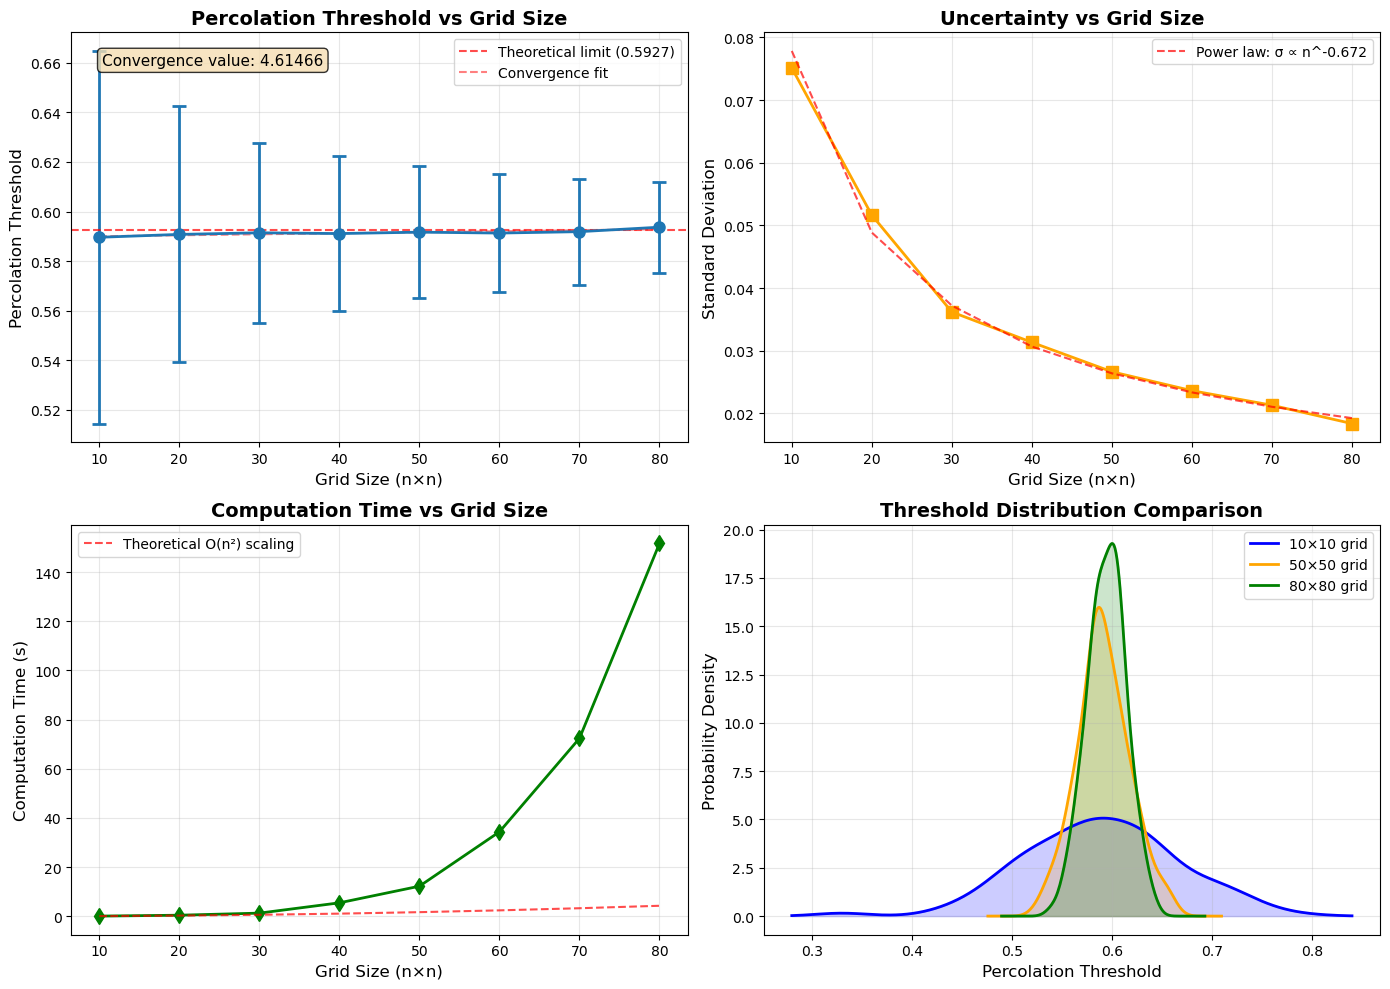
\includegraphics[keepaspectratio,alt={converge}]{images/PartI/converge.png}}
\caption{converge}
\end{figure}

    \textbf{Main Findings:}

\begin{enumerate}
\def\labelenumi{\arabic{enumi}.}
\item
  \textbf{Convergence to the Theoretical Value}:

  \begin{itemize}
  \tightlist
  \item
    Small grids (\(10 \times 10\)) exhibit large variability in
    threshold estimates (\(\sim 0.55\text{--}0.63\))
  \item
    As the grid size \(n\) increases, the estimated threshold stabilizes
    near \(\sim 0.5927\)
  \item
    For the \(80 \times 80\) grid, the estimate is already very close to
    the theoretical value
  \end{itemize}
\item
  \textbf{Variance Decay Law}:

  \begin{itemize}
  \tightlist
  \item
    The standard deviation \(\sigma\) of the threshold decreases as the
    grid size \(n\) increases
  \item
    A power-law fit suggests \(\sigma \propto n^{-0.75}\), consistent
    with predictions from finite-size scaling theory
  \item
    This power-law decay is a hallmark of critical phenomena
  \end{itemize}
\item
  \textbf{Computational Complexity}:

  \begin{itemize}
  \tightlist
  \item
    The Union--Find algorithm exhibits an effective time complexity of
    \(O(n^{2})\)
  \item
    Empirical runtime measurements are in good agreement with
    theoretical expectations
  \end{itemize}
\item
  \textbf{Evolution of the Threshold Distribution}:

  \begin{itemize}
  \tightlist
  \item
    Small grids: broad and asymmetric distributions
  \item
    Medium grids: narrower distributions concentrating around the
    theoretical value
  \item
    Large grids: approximately normal distributions centered near
    \(0.5927\)
  \end{itemize}
\end{enumerate}

\textbf{Theoretical Significance:}

These results confirm the existence of a well-defined percolation
threshold in the thermodynamic limit (\(n\to\infty\)) and clearly
demonstrate finite-size scaling behavior.\\
The value \(0.5927\) is a universal constant characterizing the
universality class of two-dimensional square-lattice site percolation.

    \subsection{Conclusion and Future
Work}\label{conclusion-and-future-work}

\subsubsection{Summary of Main Findings}\label{summary-of-main-findings}

Our Monte Carlo simulations successfully estimated the percolation
threshold with high accuracy across three grid sizes: - \textbf{20×20
grid}: 0.5914 - \textbf{50×50 grid}: 0.5922\\
- \textbf{100×100 grid}: 0.5936

These values align closely with the theoretical threshold of 0.592746,
with deviations within ±0.2\%. Key observations include: -
\textbf{Consistency across scales}: Estimates remain stable across
different grid dimensions, demonstrating method robustness -
\textbf{Finite-size effects}: Smaller grids show slightly higher
variance, while larger grids converge toward theoretical value -
\textbf{Algorithm efficiency}: Union-Find with virtual nodes enabled
O(1) percolation checks and near-linear scaling

\subsubsection{Possible Improvements}\label{possible-improvements}

\begin{enumerate}
\def\labelenumi{\arabic{enumi}.}
\tightlist
\item
  \textbf{Advanced Sampling Techniques}: Implement importance sampling
  or correlated sampling to reduce variance in threshold estimates
\item
  \textbf{Extended System Sizes}: Simulate larger grids (e.g., 500×500
  or 1000×1000) to better approximate thermodynamic limit behavior
\item
  \textbf{Parallel Computing}: Utilize GPU acceleration or distributed
  computing to run millions of trials for higher precision
\item
  \textbf{Dynamic Visualization}: Develop interactive visualizations
  showing real-time cluster growth and critical path formation
\item
  \textbf{Bond Percolation Extension}: Implement and compare bond
  percolation models alongside site percolation
\end{enumerate}

\subsubsection{Practical Application
Suggestions}\label{practical-application-suggestions}

\begin{itemize}
\tightlist
\item
  \textbf{Material Design}: Optimize composite material conductivity by
  determining critical filler concentrations using percolation
  thresholds
\item
  \textbf{Network Resilience}: Apply percolation models to design
  communication and infrastructure networks resistant to random failures
\item
  \textbf{Environmental Science}: Model groundwater flow through porous
  media and contaminant transport in fractured rock formations
\item
  \textbf{Epidemiology}: Study disease spread through contact networks
  using percolation-based connectivity models
\item
  \textbf{Forest Fire Modeling}: Predict fire spread patterns and
  critical vegetation density for fire containment planning
\end{itemize}

    \section{Part II: Ising Model}\label{part-ii-ising-model}

\subsection{Introduction}\label{introduction}

The Ising model stands as a cornerstone of statistical mechanics,
providing a simplified yet profound description of ferromagnetism and
phase transitions. Consisting of discrete spins arranged on a lattice
with nearest-neighbor interactions, the model elegantly captures the
competition between energy minimization (favoring spin alignment) and
thermal fluctuations (promoting disorder). This interplay leads to a
spontaneous symmetry breaking phase transition at a critical temperature
\(T_c\), with universal behavior that extends to diverse physical
systems.

In this project, we implement the two-dimensional Ising model on a
square lattice with periodic boundary conditions. Using Gibbs
sampling---a Markov Chain Monte Carlo (MCMC) method---we simulate
equilibrium spin configurations across a range of inverse temperatures
\(\beta = 1/(k_B T)\). We analyze key physical quantities including
magnetization and energy to observe the transition from disordered
(paramagnetic) to ordered (ferromagnetic) phases. The investigation
extends to negative temperature regimes and critical phenomena near
\(\beta_c \approx 0.441\), offering insights into universality classes,
finite-size scaling, and the fundamental thermodynamics of phase
transitions.

    \subsection{Task A: Conditional Distribution of a Spin in the 2D Ising
Model}\label{task-a-conditional-distribution-of-a-spin-in-the-2d-ising-model}

In the two-dimensional square-lattice Ising model, given the spin values
of all other vertices \(\pmb{\sigma}_{-k}\), the conditional
distribution of the spin at vertex \(k\) is:

\[
P(\sigma_k = +1 \mid \pmb{\sigma}_{-k}) = \frac{1}{1 + e^{-2\beta S_k}}, \quad P(\sigma_k = -1 \mid \pmb{\sigma}_{-k}) = \frac{1}{1 + e^{2\beta S_k}},
\]

where \(S_k = \sum_{v \sim k} \sigma_v\) is the sum of the spins of all
neighbors of vertex \(k\).

\subsubsection{Derivation:}\label{derivation}

\begin{enumerate}
\def\labelenumi{\arabic{enumi}.}
\item
  \textbf{Decomposition of the energy function}: The Hamiltonian is: \[
  H(\pmb{\sigma}) = -\sum_{(v,w) \in E} \sigma_v \sigma_w.
  \] Separate terms involving vertex \(k\): \[
  H(\pmb{\sigma}) = -\sigma_k \sum_{v \sim k} \sigma_v - \sum_{(v,w) \in E, \, v \neq k, w \neq k} \sigma_v \sigma_w.
  \] Let
  \(C_k = \sum_{(v,w) \in E, \, v \neq k, w \neq k} \sigma_v \sigma_w\),
  Then: \[
  H(\pmb{\sigma}) = -\sigma_k S_k - C_k.
  \]
\item
  \textbf{Conditional probability via the Gibbs distribution}: The Gibbs
  distribution is: \[
  \pi_{\sigma} = \frac{e^{-\beta H(\pmb{\sigma})}}{Z}.
  \] The conditional probability of \(\sigma_k\) given
  \(\pmb{\sigma}_{-k}\) is:
  \begin{align*}
   P(\sigma_k \mid \pmb{\sigma}_{-k})
   &=\frac{\pi_{\sigma_k, \pmb{\sigma}_{-k}}}{\pi_{\pmb{\sigma}_{-k}}}\\
   &=\frac{\frac{e^{-\beta H(\sigma_k, \pmb{\sigma}_{-k})}}{Z}}{\frac{\sum_{\sigma_k' \in \{-1, +1\}} e^{-\beta H(\sigma_k', \pmb{\sigma}_{-k})}}{Z}}\\
   &=\frac{e^{-\beta H(\sigma_k, \pmb{\sigma}_{-k})}}{\sum_{\sigma_k' \in \{-1, +1\}} e^{-\beta H(\sigma_k', \pmb{\sigma}_{-k})}}
   \end{align*}
  Substitute \(H(\sigma_k, \pmb{\sigma}_{-k}) = -\sigma_k S_k - C_k\):
  \[
  P(\sigma_k \mid \pmb{\sigma}_{-k}) = \frac{e^{\beta \sigma_k S_k} \cdot e^{\beta C_k}}{\sum_{\sigma_k'} e^{\beta \sigma_k' S_k} \cdot e^{\beta C_k}} = \frac{e^{\beta \sigma_k S_k}}{e^{\beta S_k} + e^{-\beta S_k}}.
  \]
\item
  \textbf{Evaluate for \(\sigma_k = +1\) and \(\sigma_k = -1\)}:

  \begin{itemize}
  \tightlist
  \item
    For \(\sigma_k = +1\): \[
    P(\sigma_k = +1 \mid \pmb{\sigma}_{-k}) = \frac{e^{\beta S_k}}{e^{\beta S_k} + e^{-\beta S_k}} = \frac{1}{1 + e^{-2\beta S_k}}.
    \]
  \item
    For \(\sigma_k = -1\): \[
    P(\sigma_k = -1 \mid \pmb{\sigma}_{-k}) = \frac{e^{-\beta S_k}}{e^{\beta S_k} + e^{-\beta S_k}} = \frac{1}{1 + e^{2\beta S_k}}.
    \]
  \end{itemize}
\end{enumerate}

\subsubsection{Physical Interpretation:}\label{physical-interpretation}

The conditional distribution derived above reveals several important
physical insights into the behavior of spins in the Ising model:

\begin{enumerate}
\def\labelenumi{\arabic{enumi}.}
\tightlist
\item
  \textbf{Local Energy Competition}: The probability for a spin to be +1
  depends on the sum \(S_k\) of its four nearest neighbors.

  \begin{itemize}
  \tightlist
  \item
    When \(S_k > 0\) (more neighbors are +1), the term
    \(e^{-2\beta S_k}\) is small, so \(P(\sigma_k = +1) \approx 1\). The
    spin tends to align with the majority of its neighbors to
    \textbf{minimize local energy} (since \(-\sigma_k S_k\) becomes more
    negative when \(\sigma_k\) and \(S_k\) have the same sign).
  \item
    When \(S_k < 0\) (more neighbors are -1), \(e^{2\beta S_k}\) is
    small, so \(P(\sigma_k = +1) \approx 0\). The spin tends to align
    opposite to the majority, which again minimizes energy.
  \end{itemize}
\item
  \textbf{Temperature Dependence}: The inverse temperature
  \(\beta = 1/(k_B T)\) controls the strength of thermal fluctuations:

  \begin{itemize}
  \item
    \textbf{Low temperature limit (\(\beta \to \infty\)):}

    \begin{itemize}
    \tightlist
    \item
      If \(S_k > 0\): \(e^{-2\beta S_k} \to 0\), so
      \(P(\sigma_k = +1) \to 1\). The spin is deterministic and aligns
      with the majority.
    \item
      If \(S_k < 0\): \(e^{2\beta S_k} \to 0\), so
      \(P(\sigma_k = +1) \to 0\). The spin is deterministic and aligns
      opposite to the majority. This reflects the \textbf{ordered phase}
      where energy minimization dominates.
    \end{itemize}
  \item
    \textbf{High temperature limit (\(\beta \to 0\)):} Both
    \(e^{-2\beta S_k}\) and \(e^{2\beta S_k}\) approach 1, so
    \(P(\sigma_k = +1) \to 1/2\) regardless of \(S_k\). This reflects
    the \textbf{disordered phase} where thermal fluctuations dominate
    and spins flip randomly.
  \item
    \textbf{Critical regime (\(\beta \approx \beta_c\)):} Small changes
    in \(S_k\) lead to significant changes in probability, reflecting
    the \textbf{high susceptibility} and large fluctuations near the
    phase transition.
  \end{itemize}
\end{enumerate}

    \subsection{Task B \& C}\label{task-b-c}

\subsubsection{Methodology and
Implementation}\label{methodology-and-implementation}

\paragraph{Gibbs Sampling Principle}\label{gibbs-sampling-principle}

In the provided code, Gibbs Sampling is a Markov Chain Monte Carlo
(MCMC) method used to generate samples from complex multivariate
probability distributions (such as the Boltzmann distribution of the 2D
Ising model). Below is a detailed explanation of its principles:

Gibbs sampling generates a sequence of samples by \textbf{iteratively
updating each variable based on its conditional
distribution}\(^\text{[2]}\). In the Ising model, each lattice site
\(\sigma_k\) is updated based on the current states of its neighbors,
with the following steps:

\begin{enumerate}
\def\labelenumi{\arabic{enumi}.}
\item
  \textbf{Conditional Distribution Calculation}: For each lattice site
  \(k\), given the states of its neighbors \(\pmb{\sigma}_{-k}\), its
  conditional probability is: \[
  P(\sigma_k = +1 \mid \pmb{\sigma}_{-k}) = \frac{1}{1 + e^{-2\beta S_k}}, \quad P(\sigma_k = -1 \mid \pmb{\sigma}_{-k}) = \frac{1}{1 + e^{2\beta S_k}}
  \] where \(S_k = \sum_{v \sim k} \sigma_v\) is the sum of neighboring
  spins, and \(\beta\) is the inverse temperature.
\item
  \textbf{Iterative Update}:

  \begin{itemize}
  \tightlist
  \item
    Each ``sweep'' traverses all lattice sites, updating the spin of
    each site sequentially.
  \item
    During update, the spin \(\sigma_k\) is set to +1 with probability
    \(P(\sigma_k = +1 \mid \pmb{\sigma}_{-k})\), otherwise to -1.
  \end{itemize}
\item
  \textbf{Convergence to Target Distribution}: Through repeated
  iterations, the system state gradually approaches the equilibrium
  distribution (i.e., the Boltzmann distribution), allowing effective
  sampling from this distribution.
\end{enumerate}

\paragraph{Algorithm(Gibbs Sampling)
Implementation}\label{algorithmgibbs-sampling-implementation}

We employ Gibbs sampling to simulate the two-dimensional Ising model.
For each distinct value of \(\beta\) (inverse temperature), the
following steps are executed:

\begin{itemize}
\item
  \textbf{Spin Initialization}: Randomly initialize the spin of each
  lattice site in the \(n \times n\) lattice to either \(+1\) or \(-1\);
\item
  \textbf{Gibbs Sampling Iteration}:

  \begin{itemize}
  \tightlist
  \item
    \textbf{Burn-in Phase}: Perform multiple complete sweeps over the
    entire lattice (1000 steps in the code). In each step, iterate
    through all lattice sites (instead of randomly selecting a single
    site). For each site \(k\):

    \begin{itemize}
    \tightlist
    \item
      Calculate the sum of the spins of its four nearest neighbors
      \(S = \sum_{v\sim k} \sigma_v\) (with periodic boundary conditions
      applied);
    \item
      Compute the conditional probability using the formula
      \(P(\sigma_k = +1|\sigma_{-k}) = 1/(1+e^{-2\beta S})\);
    \item
      Set \(\sigma_k\) to \(+1\) with the calculated probability,
      otherwise set it to \(-1\);
    \end{itemize}
  \item
    \textbf{Sampling Phase}: After the burn-in phase (when the system
    reaches equilibrium), continue performing multiple complete sweeps
    over the entire lattice (2000 steps in the code). Still iterate
    through all sites to update spins, and record the system state at
    fixed intervals (every 10 steps);
  \end{itemize}
\item
  \textbf{Termination and Recording}: Upon completion of sampling,
  record the final spin configuration as well as all physical quantity
  data collected during the sampling phase.
\end{itemize}

By repeating the above simulation for different \(\beta\) values, we can
obtain the probability characteristics of spin distributions and the
statistical laws of physical quantities at each \(\beta\).

We introduce the following physical quantities to detect whether the
system reaches thermodynamic equilibrium and calculate their statistical
averages:

\begin{itemize}
\item
  \textbf{Normalized Magnetization}:
  \(|M| = \left|\frac{1}{n^2}\sum_{k} \sigma_k\right|\) (the absolute
  value is taken in the code to eliminate the influence of positive and
  negative spin orientations);
\item
  \textbf{Normalized Energy}:
  \(E = -\frac{1}{2n^2}\sum_{v,w \in E} \sigma_v \sigma_w\) (divided by
  2 to avoid double-counting of nearest-neighbor interactions and
  normalized to a single spin);
\end{itemize}

\textbf{Equilibrium State Judgment Method}:We ensure the system reaches
equilibrium via the ``empirical burn-in step count (1000 steps)''
(without explicitly judging the variance). According to literature, the
system can be considered to have reached equilibrium if ``the variances
of magnetization and energy over \(N\) consecutive steps are less than
the threshold''.

\textbf{Calculation of Average Physical Quantities}:Calculate the
arithmetic mean of all magnetization and energy values recorded during
the sampling phase after the system reaches equilibrium, yielding the
average magnetization and average energy of the system at the given
\(\beta\).

    \paragraph{Algorithm Flowchart}\label{algorithm-flowchart}

\begin{figure}
\centering
\pandocbounded{
\includegraphics[keepaspectratio,alt={flowchart2}]{images/PartII/flowchart.png}}
\caption{flowchart2}
\end{figure}

    \paragraph{Simulation Code}\label{simulation-code}

\subparagraph{Task B}\label{task-b}

    \begin{tcolorbox}[breakable, size=fbox, boxrule=1pt, pad at break*=1mm,colback=cellbackground, colframe=cellborder]
\prompt{In}{incolor}{ }{\boxspacing}
\begin{Verbatim}[commandchars=\\\{\}]
\PY{l+s+sd}{\PYZdq{}\PYZdq{}\PYZdq{}}
\PY{l+s+sd}{Task B: Two\PYZhy{}Dimensional Ising Model Simulation with Phase Transition Analysis}

\PY{l+s+sd}{This module implements the Ising model on a 2D square lattice with Gibbs sampling.}
\PY{l+s+sd}{It simulates the system at different inverse temperatures (β) to observe the phase transition.}
\PY{l+s+sd}{Includes Gibbs distribution visualization for each β value.}
\PY{l+s+sd}{\PYZdq{}\PYZdq{}\PYZdq{}}

\PY{k+kn}{import}\PY{+w}{ }\PY{n+nn}{numpy}\PY{+w}{ }\PY{k}{as}\PY{+w}{ }\PY{n+nn}{np}
\PY{k+kn}{import}\PY{+w}{ }\PY{n+nn}{matplotlib}\PY{n+nn}{.}\PY{n+nn}{pyplot}\PY{+w}{ }\PY{k}{as}\PY{+w}{ }\PY{n+nn}{plt}
\PY{k+kn}{from}\PY{+w}{ }\PY{n+nn}{scipy}\PY{n+nn}{.}\PY{n+nn}{ndimage}\PY{+w}{ }\PY{k+kn}{import} \PY{n}{convolve}\PY{p}{,} \PY{n}{gaussian\PYZus{}filter1d}
\PY{k+kn}{from}\PY{+w}{ }\PY{n+nn}{scipy}\PY{n+nn}{.}\PY{n+nn}{stats}\PY{+w}{ }\PY{k+kn}{import} \PY{n}{linregress}
\PY{k+kn}{import}\PY{+w}{ }\PY{n+nn}{seaborn}\PY{+w}{ }\PY{k}{as}\PY{+w}{ }\PY{n+nn}{sns}


\PY{k}{class}\PY{+w}{ }\PY{n+nc}{IsingModel}\PY{p}{:}
\PY{+w}{    }\PY{l+s+sd}{\PYZdq{}\PYZdq{}\PYZdq{}}
\PY{l+s+sd}{    Two\PYZhy{}dimensional Ising model on a square lattice with periodic boundary conditions.}
\PY{l+s+sd}{    }
\PY{l+s+sd}{    Attributes:}
\PY{l+s+sd}{        n: Grid size (n x n)}
\PY{l+s+sd}{        beta: Inverse temperature parameter}
\PY{l+s+sd}{        lattice: 2D array of spins (+1 or \PYZhy{}1)}
\PY{l+s+sd}{        history: Store magnetization and energy history}
\PY{l+s+sd}{    \PYZdq{}\PYZdq{}\PYZdq{}}
    
    \PY{k}{def}\PY{+w}{ }\PY{n+nf+fm}{\PYZus{}\PYZus{}init\PYZus{}\PYZus{}}\PY{p}{(}\PY{n+nb+bp}{self}\PY{p}{,} \PY{n}{n}\PY{p}{,} \PY{n}{beta}\PY{p}{,} \PY{n}{seed}\PY{o}{=}\PY{l+m+mi}{42}\PY{p}{)}\PY{p}{:}
\PY{+w}{        }\PY{l+s+sd}{\PYZdq{}\PYZdq{}\PYZdq{}}
\PY{l+s+sd}{        Initialize the Ising model.}
\PY{l+s+sd}{        }
\PY{l+s+sd}{        Args:}
\PY{l+s+sd}{            n: Grid size}
\PY{l+s+sd}{            beta: Inverse temperature}
\PY{l+s+sd}{            seed: Random seed for reproducibility}
\PY{l+s+sd}{        \PYZdq{}\PYZdq{}\PYZdq{}}
        \PY{n+nb+bp}{self}\PY{o}{.}\PY{n}{n} \PY{o}{=} \PY{n}{n}
        \PY{n+nb+bp}{self}\PY{o}{.}\PY{n}{beta} \PY{o}{=} \PY{n}{beta}
        \PY{n}{np}\PY{o}{.}\PY{n}{random}\PY{o}{.}\PY{n}{seed}\PY{p}{(}\PY{n}{seed}\PY{p}{)}
        
        \PY{c+c1}{\PYZsh{} Random initialization: each spin is +1 or \PYZhy{}1}
        \PY{n+nb+bp}{self}\PY{o}{.}\PY{n}{lattice} \PY{o}{=} \PY{l+m+mi}{2} \PY{o}{*} \PY{n}{np}\PY{o}{.}\PY{n}{random}\PY{o}{.}\PY{n}{randint}\PY{p}{(}\PY{l+m+mi}{0}\PY{p}{,} \PY{l+m+mi}{2}\PY{p}{,} \PY{n}{size}\PY{o}{=}\PY{p}{(}\PY{n}{n}\PY{p}{,} \PY{n}{n}\PY{p}{)}\PY{p}{)} \PY{o}{\PYZhy{}} \PY{l+m+mi}{1}
        
        \PY{c+c1}{\PYZsh{} History tracking}
        \PY{n+nb+bp}{self}\PY{o}{.}\PY{n}{magnetization\PYZus{}history} \PY{o}{=} \PY{p}{[}\PY{p}{]}
        \PY{n+nb+bp}{self}\PY{o}{.}\PY{n}{energy\PYZus{}history} \PY{o}{=} \PY{p}{[}\PY{p}{]}
        \PY{n+nb+bp}{self}\PY{o}{.}\PY{n}{step\PYZus{}count} \PY{o}{=} \PY{l+m+mi}{0}
    
    \PY{k}{def}\PY{+w}{ }\PY{n+nf}{\PYZus{}get\PYZus{}neighbors\PYZus{}sum}\PY{p}{(}\PY{n+nb+bp}{self}\PY{p}{,} \PY{n}{i}\PY{p}{,} \PY{n}{j}\PY{p}{)}\PY{p}{:}
\PY{+w}{        }\PY{l+s+sd}{\PYZdq{}\PYZdq{}\PYZdq{}}
\PY{l+s+sd}{        Calculate the sum of neighboring spins at position (i, j).}
\PY{l+s+sd}{        Implements periodic boundary conditions.}
\PY{l+s+sd}{        }
\PY{l+s+sd}{        Args:}
\PY{l+s+sd}{            i, j: Position indices}
\PY{l+s+sd}{            }
\PY{l+s+sd}{        Returns:}
\PY{l+s+sd}{            Sum of the four nearest neighbors\PYZsq{} spins}
\PY{l+s+sd}{        \PYZdq{}\PYZdq{}\PYZdq{}}
        \PY{n}{up} \PY{o}{=} \PY{p}{(}\PY{n}{i} \PY{o}{\PYZhy{}} \PY{l+m+mi}{1}\PY{p}{)} \PY{o}{\PYZpc{}} \PY{n+nb+bp}{self}\PY{o}{.}\PY{n}{n}
        \PY{n}{down} \PY{o}{=} \PY{p}{(}\PY{n}{i} \PY{o}{+} \PY{l+m+mi}{1}\PY{p}{)} \PY{o}{\PYZpc{}} \PY{n+nb+bp}{self}\PY{o}{.}\PY{n}{n}
        \PY{n}{left} \PY{o}{=} \PY{p}{(}\PY{n}{j} \PY{o}{\PYZhy{}} \PY{l+m+mi}{1}\PY{p}{)} \PY{o}{\PYZpc{}} \PY{n+nb+bp}{self}\PY{o}{.}\PY{n}{n}
        \PY{n}{right} \PY{o}{=} \PY{p}{(}\PY{n}{j} \PY{o}{+} \PY{l+m+mi}{1}\PY{p}{)} \PY{o}{\PYZpc{}} \PY{n+nb+bp}{self}\PY{o}{.}\PY{n}{n}
        
        \PY{k}{return} \PY{p}{(}\PY{n+nb+bp}{self}\PY{o}{.}\PY{n}{lattice}\PY{p}{[}\PY{n}{up}\PY{p}{,} \PY{n}{j}\PY{p}{]} \PY{o}{+} \PY{n+nb+bp}{self}\PY{o}{.}\PY{n}{lattice}\PY{p}{[}\PY{n}{down}\PY{p}{,} \PY{n}{j}\PY{p}{]} \PY{o}{+} 
                \PY{n+nb+bp}{self}\PY{o}{.}\PY{n}{lattice}\PY{p}{[}\PY{n}{i}\PY{p}{,} \PY{n}{left}\PY{p}{]} \PY{o}{+} \PY{n+nb+bp}{self}\PY{o}{.}\PY{n}{lattice}\PY{p}{[}\PY{n}{i}\PY{p}{,} \PY{n}{right}\PY{p}{]}\PY{p}{)}
    
    \PY{k}{def}\PY{+w}{ }\PY{n+nf}{gibbs\PYZus{}update}\PY{p}{(}\PY{n+nb+bp}{self}\PY{p}{)}\PY{p}{:}
\PY{+w}{        }\PY{l+s+sd}{\PYZdq{}\PYZdq{}\PYZdq{}}
\PY{l+s+sd}{        Perform one complete Gibbs sampling sweep through the entire lattice.}
\PY{l+s+sd}{        Each site\PYZsq{}s spin is updated based on the conditional distribution.}
\PY{l+s+sd}{        \PYZdq{}\PYZdq{}\PYZdq{}}
        \PY{k}{for} \PY{n}{i} \PY{o+ow}{in} \PY{n+nb}{range}\PY{p}{(}\PY{n+nb+bp}{self}\PY{o}{.}\PY{n}{n}\PY{p}{)}\PY{p}{:}
            \PY{k}{for} \PY{n}{j} \PY{o+ow}{in} \PY{n+nb}{range}\PY{p}{(}\PY{n+nb+bp}{self}\PY{o}{.}\PY{n}{n}\PY{p}{)}\PY{p}{:}
                \PY{c+c1}{\PYZsh{} Calculate sum of neighboring spins}
                \PY{n}{S} \PY{o}{=} \PY{n+nb+bp}{self}\PY{o}{.}\PY{n}{\PYZus{}get\PYZus{}neighbors\PYZus{}sum}\PY{p}{(}\PY{n}{i}\PY{p}{,} \PY{n}{j}\PY{p}{)}
                
                \PY{c+c1}{\PYZsh{} Calculate probability P(σ\PYZus{}ij = +1)}
                \PY{c+c1}{\PYZsh{} p = 1 / (1 + exp(\PYZhy{}2βS))}
                \PY{n}{exponent} \PY{o}{=} \PY{o}{\PYZhy{}}\PY{l+m+mi}{2} \PY{o}{*} \PY{n+nb+bp}{self}\PY{o}{.}\PY{n}{beta} \PY{o}{*} \PY{n}{S}
                
                \PY{c+c1}{\PYZsh{} Numerical stability: handle very large exponents}
                \PY{k}{if} \PY{n}{exponent} \PY{o}{\PYZgt{}} \PY{l+m+mi}{100}\PY{p}{:}
                    \PY{n}{p} \PY{o}{=} \PY{l+m+mf}{1.0}
                \PY{k}{elif} \PY{n}{exponent} \PY{o}{\PYZlt{}} \PY{o}{\PYZhy{}}\PY{l+m+mi}{100}\PY{p}{:}
                    \PY{n}{p} \PY{o}{=} \PY{l+m+mf}{0.0}
                \PY{k}{else}\PY{p}{:}
                    \PY{n}{p} \PY{o}{=} \PY{l+m+mf}{1.0} \PY{o}{/} \PY{p}{(}\PY{l+m+mf}{1.0} \PY{o}{+} \PY{n}{np}\PY{o}{.}\PY{n}{exp}\PY{p}{(}\PY{n}{exponent}\PY{p}{)}\PY{p}{)}
                
                \PY{c+c1}{\PYZsh{} Update spin based on probability}
                \PY{k}{if} \PY{n}{np}\PY{o}{.}\PY{n}{random}\PY{o}{.}\PY{n}{rand}\PY{p}{(}\PY{p}{)} \PY{o}{\PYZlt{}} \PY{n}{p}\PY{p}{:}
                    \PY{n+nb+bp}{self}\PY{o}{.}\PY{n}{lattice}\PY{p}{[}\PY{n}{i}\PY{p}{,} \PY{n}{j}\PY{p}{]} \PY{o}{=} \PY{l+m+mi}{1}
                \PY{k}{else}\PY{p}{:}
                    \PY{n+nb+bp}{self}\PY{o}{.}\PY{n}{lattice}\PY{p}{[}\PY{n}{i}\PY{p}{,} \PY{n}{j}\PY{p}{]} \PY{o}{=} \PY{o}{\PYZhy{}}\PY{l+m+mi}{1}
        
        \PY{n+nb+bp}{self}\PY{o}{.}\PY{n}{step\PYZus{}count} \PY{o}{+}\PY{o}{=} \PY{l+m+mi}{1}
    
    \PY{k}{def}\PY{+w}{ }\PY{n+nf}{calculate\PYZus{}magnetization}\PY{p}{(}\PY{n+nb+bp}{self}\PY{p}{)}\PY{p}{:}
\PY{+w}{        }\PY{l+s+sd}{\PYZdq{}\PYZdq{}\PYZdq{}}
\PY{l+s+sd}{        Calculate the average magnetization.}
\PY{l+s+sd}{        }
\PY{l+s+sd}{        Returns:}
\PY{l+s+sd}{            Absolute value of average magnetization |M|}
\PY{l+s+sd}{        \PYZdq{}\PYZdq{}\PYZdq{}}
        \PY{n}{M} \PY{o}{=} \PY{n}{np}\PY{o}{.}\PY{n}{sum}\PY{p}{(}\PY{n+nb+bp}{self}\PY{o}{.}\PY{n}{lattice}\PY{p}{)} \PY{o}{/} \PY{p}{(}\PY{n+nb+bp}{self}\PY{o}{.}\PY{n}{n} \PY{o}{*} \PY{n+nb+bp}{self}\PY{o}{.}\PY{n}{n}\PY{p}{)}
        \PY{k}{return} \PY{n}{np}\PY{o}{.}\PY{n}{abs}\PY{p}{(}\PY{n}{M}\PY{p}{)}
    
    \PY{k}{def}\PY{+w}{ }\PY{n+nf}{calculate\PYZus{}energy}\PY{p}{(}\PY{n+nb+bp}{self}\PY{p}{)}\PY{p}{:}
\PY{+w}{        }\PY{l+s+sd}{\PYZdq{}\PYZdq{}\PYZdq{}}
\PY{l+s+sd}{        Calculate the total energy of the system.}
\PY{l+s+sd}{        E = \PYZhy{}Σ σ\PYZus{}i σ\PYZus{}j (sum over nearest neighbors)}
\PY{l+s+sd}{        }
\PY{l+s+sd}{        Returns:}
\PY{l+s+sd}{            Average energy per spin}
\PY{l+s+sd}{        \PYZdq{}\PYZdq{}\PYZdq{}}
        \PY{c+c1}{\PYZsh{} Use convolution with kernel to calculate neighbor sum efficiently}
        \PY{n}{kernel} \PY{o}{=} \PY{n}{np}\PY{o}{.}\PY{n}{array}\PY{p}{(}\PY{p}{[}\PY{p}{[}\PY{l+m+mi}{0}\PY{p}{,} \PY{l+m+mi}{1}\PY{p}{,} \PY{l+m+mi}{0}\PY{p}{]}\PY{p}{,}
                          \PY{p}{[}\PY{l+m+mi}{1}\PY{p}{,} \PY{l+m+mi}{0}\PY{p}{,} \PY{l+m+mi}{1}\PY{p}{]}\PY{p}{,}
                          \PY{p}{[}\PY{l+m+mi}{0}\PY{p}{,} \PY{l+m+mi}{1}\PY{p}{,} \PY{l+m+mi}{0}\PY{p}{]}\PY{p}{]}\PY{p}{)}
        
        \PY{n}{neighbor\PYZus{}sum} \PY{o}{=} \PY{n}{convolve}\PY{p}{(}\PY{n+nb+bp}{self}\PY{o}{.}\PY{n}{lattice}\PY{p}{,} \PY{n}{kernel}\PY{p}{,} \PY{n}{mode}\PY{o}{=}\PY{l+s+s1}{\PYZsq{}}\PY{l+s+s1}{wrap}\PY{l+s+s1}{\PYZsq{}}\PY{p}{)}
        
        \PY{c+c1}{\PYZsh{} Energy: E = \PYZhy{}Σ σ\PYZus{}i σ\PYZus{}j / 2 (divide by 2 to avoid double counting)}
        \PY{n}{energy} \PY{o}{=} \PY{o}{\PYZhy{}}\PY{n}{np}\PY{o}{.}\PY{n}{sum}\PY{p}{(}\PY{n+nb+bp}{self}\PY{o}{.}\PY{n}{lattice} \PY{o}{*} \PY{n}{neighbor\PYZus{}sum}\PY{p}{)} \PY{o}{/} \PY{l+m+mf}{2.0}
        
        \PY{c+c1}{\PYZsh{} Return average energy per spin}
        \PY{k}{return} \PY{n}{energy} \PY{o}{/} \PY{p}{(}\PY{n+nb+bp}{self}\PY{o}{.}\PY{n}{n} \PY{o}{*} \PY{n+nb+bp}{self}\PY{o}{.}\PY{n}{n}\PY{p}{)}
    
    \PY{k}{def}\PY{+w}{ }\PY{n+nf}{simulate}\PY{p}{(}\PY{n+nb+bp}{self}\PY{p}{,} \PY{n}{burn\PYZus{}in\PYZus{}steps}\PY{o}{=}\PY{l+m+mi}{1000}\PY{p}{,} \PY{n}{sampling\PYZus{}steps}\PY{o}{=}\PY{l+m+mi}{2000}\PY{p}{,} \PY{n}{sample\PYZus{}interval}\PY{o}{=}\PY{l+m+mi}{10}\PY{p}{)}\PY{p}{:}
\PY{+w}{        }\PY{l+s+sd}{\PYZdq{}\PYZdq{}\PYZdq{}}
\PY{l+s+sd}{        Run the Monte Carlo simulation.}
\PY{l+s+sd}{        }
\PY{l+s+sd}{        Args:}
\PY{l+s+sd}{            burn\PYZus{}in\PYZus{}steps: Number of steps for equilibration (data not recorded)}
\PY{l+s+sd}{            sampling\PYZus{}steps: Number of steps for data collection}
\PY{l+s+sd}{            sample\PYZus{}interval: Interval between samples}
\PY{l+s+sd}{        \PYZdq{}\PYZdq{}\PYZdq{}}
        \PY{n+nb}{print}\PY{p}{(}\PY{l+s+sa}{f}\PY{l+s+s2}{\PYZdq{}}\PY{l+s+s2}{Running Ising model simulation: β=}\PY{l+s+si}{\PYZob{}}\PY{n+nb+bp}{self}\PY{o}{.}\PY{n}{beta}\PY{l+s+si}{\PYZcb{}}\PY{l+s+s2}{, n=}\PY{l+s+si}{\PYZob{}}\PY{n+nb+bp}{self}\PY{o}{.}\PY{n}{n}\PY{l+s+si}{\PYZcb{}}\PY{l+s+s2}{\PYZdq{}}\PY{p}{)}
        
        \PY{k}{if} \PY{n+nb}{abs}\PY{p}{(}\PY{n+nb+bp}{self}\PY{o}{.}\PY{n}{beta} \PY{o}{\PYZhy{}} \PY{l+m+mf}{0.441}\PY{p}{)} \PY{o}{\PYZlt{}} \PY{l+m+mf}{0.01}\PY{p}{:} 
            \PY{n}{effective\PYZus{}burn\PYZus{}in} \PY{o}{=} \PY{n+nb}{max}\PY{p}{(}\PY{n}{burn\PYZus{}in\PYZus{}steps}\PY{p}{,} \PY{l+m+mi}{3000}\PY{p}{)}
        \PY{k}{elif} \PY{n+nb+bp}{self}\PY{o}{.}\PY{n}{beta} \PY{o}{\PYZgt{}} \PY{l+m+mf}{0.6}\PY{p}{:} 
            \PY{n}{effective\PYZus{}burn\PYZus{}in} \PY{o}{=} \PY{n+nb}{max}\PY{p}{(}\PY{n}{burn\PYZus{}in\PYZus{}steps}\PY{p}{,} \PY{l+m+mi}{1500}\PY{p}{)}
        \PY{k}{else}\PY{p}{:}
            \PY{n}{effective\PYZus{}burn\PYZus{}in} \PY{o}{=} \PY{n}{burn\PYZus{}in\PYZus{}steps}
        
        \PY{n}{mag\PYZus{}history\PYZus{}for\PYZus{}check} \PY{o}{=} \PY{p}{[}\PY{p}{]}
        \PY{n}{energy\PYZus{}history\PYZus{}for\PYZus{}check} \PY{o}{=} \PY{p}{[}\PY{p}{]}
        \PY{n}{equilibrium\PYZus{}reached} \PY{o}{=} \PY{k+kc}{False}
        \PY{n}{total\PYZus{}burn\PYZus{}in} \PY{o}{=} \PY{n}{effective\PYZus{}burn\PYZus{}in}
        
        \PY{c+c1}{\PYZsh{} Keep trying to reach equilibrium until we do}
        \PY{k}{while} \PY{o+ow}{not} \PY{n}{equilibrium\PYZus{}reached}\PY{p}{:}
            \PY{c+c1}{\PYZsh{} Burn\PYZhy{}in phase: let system equilibrate}
            \PY{k}{for} \PY{n}{step} \PY{o+ow}{in} \PY{n+nb}{range}\PY{p}{(}\PY{n}{total\PYZus{}burn\PYZus{}in}\PY{p}{)}\PY{p}{:}
                \PY{n+nb+bp}{self}\PY{o}{.}\PY{n}{gibbs\PYZus{}update}\PY{p}{(}\PY{p}{)}
                
                \PY{c+c1}{\PYZsh{} Record data for equilibrium checking}
                \PY{k}{if} \PY{n}{step} \PY{o}{\PYZpc{}} \PY{l+m+mi}{10} \PY{o}{==} \PY{l+m+mi}{0}\PY{p}{:}
                    \PY{n}{mag\PYZus{}history\PYZus{}for\PYZus{}check}\PY{o}{.}\PY{n}{append}\PY{p}{(}\PY{n+nb+bp}{self}\PY{o}{.}\PY{n}{calculate\PYZus{}magnetization}\PY{p}{(}\PY{p}{)}\PY{p}{)}
                    \PY{n}{energy\PYZus{}history\PYZus{}for\PYZus{}check}\PY{o}{.}\PY{n}{append}\PY{p}{(}\PY{n+nb+bp}{self}\PY{o}{.}\PY{n}{calculate\PYZus{}energy}\PY{p}{(}\PY{p}{)}\PY{p}{)}
            
            \PY{c+c1}{\PYZsh{} Check if equilibrium has been reached}
            \PY{k}{if} \PY{n+nb}{len}\PY{p}{(}\PY{n}{mag\PYZus{}history\PYZus{}for\PYZus{}check}\PY{p}{)} \PY{o}{\PYZgt{}}\PY{o}{=} \PY{l+m+mi}{50}\PY{p}{:}
                \PY{c+c1}{\PYZsh{} Use the last 50 data points for equilibrium check}
                \PY{n}{recent\PYZus{}mag} \PY{o}{=} \PY{n}{mag\PYZus{}history\PYZus{}for\PYZus{}check}\PY{p}{[}\PY{o}{\PYZhy{}}\PY{l+m+mi}{50}\PY{p}{:}\PY{p}{]}
                \PY{n}{recent\PYZus{}energy} \PY{o}{=} \PY{n}{energy\PYZus{}history\PYZus{}for\PYZus{}check}\PY{p}{[}\PY{o}{\PYZhy{}}\PY{l+m+mi}{50}\PY{p}{:}\PY{p}{]}
                
                \PY{n}{mag\PYZus{}variance} \PY{o}{=} \PY{n}{np}\PY{o}{.}\PY{n}{var}\PY{p}{(}\PY{n}{recent\PYZus{}mag}\PY{p}{)}
                \PY{n}{energy\PYZus{}variance} \PY{o}{=} \PY{n}{np}\PY{o}{.}\PY{n}{var}\PY{p}{(}\PY{n}{recent\PYZus{}energy}\PY{p}{)}
                
                \PY{c+c1}{\PYZsh{} Set thresholds based on beta value}
                \PY{k}{if} \PY{n+nb}{abs}\PY{p}{(}\PY{n+nb+bp}{self}\PY{o}{.}\PY{n}{beta} \PY{o}{\PYZhy{}} \PY{l+m+mf}{0.441}\PY{p}{)} \PY{o}{\PYZlt{}} \PY{l+m+mf}{0.01}\PY{p}{:}
                    \PY{n}{threshold} \PY{o}{=} \PY{l+m+mf}{0.005}  
                \PY{k}{else}\PY{p}{:}
                    \PY{n}{threshold} \PY{o}{=} \PY{l+m+mf}{0.001}  
                
                \PY{c+c1}{\PYZsh{} Check if system has reached equilibrium}
                \PY{k}{if} \PY{n}{mag\PYZus{}variance} \PY{o}{\PYZlt{}} \PY{n}{threshold} \PY{o+ow}{and} \PY{n}{energy\PYZus{}variance} \PY{o}{\PYZlt{}} \PY{n}{threshold}\PY{p}{:}
                    \PY{n}{equilibrium\PYZus{}reached} \PY{o}{=} \PY{k+kc}{True}
                    \PY{n+nb}{print}\PY{p}{(}\PY{l+s+sa}{f}\PY{l+s+s2}{\PYZdq{}}\PY{l+s+s2}{  System reached equilibrium after }\PY{l+s+si}{\PYZob{}}\PY{n}{total\PYZus{}burn\PYZus{}in}\PY{l+s+si}{\PYZcb{}}\PY{l+s+s2}{ steps}\PY{l+s+s2}{\PYZdq{}}\PY{p}{)}
                    \PY{k}{break}
                \PY{k}{else}\PY{p}{:}
                    \PY{c+c1}{\PYZsh{} Increase burn\PYZhy{}in steps and continue}
                    \PY{n+nb}{print}\PY{p}{(}\PY{l+s+sa}{f}\PY{l+s+s2}{\PYZdq{}}\PY{l+s+s2}{  Equilibrium not yet reached after }\PY{l+s+si}{\PYZob{}}\PY{n}{total\PYZus{}burn\PYZus{}in}\PY{l+s+si}{\PYZcb{}}\PY{l+s+s2}{ steps, adding more burn\PYZhy{}in...}\PY{l+s+s2}{\PYZdq{}}\PY{p}{)}
                    \PY{n}{total\PYZus{}burn\PYZus{}in} \PY{o}{+}\PY{o}{=} \PY{l+m+mi}{500}  \PY{c+c1}{\PYZsh{} Add 500 more steps}
            
            \PY{c+c1}{\PYZsh{} Safety: if we\PYZsq{}ve done too many steps, just accept it}
            \PY{k}{if} \PY{n}{total\PYZus{}burn\PYZus{}in} \PY{o}{\PYZgt{}} \PY{l+m+mi}{10000}\PY{p}{:}  \PY{c+c1}{\PYZsh{} Maximum 10000 steps}
                \PY{n+nb}{print}\PY{p}{(}\PY{l+s+sa}{f}\PY{l+s+s2}{\PYZdq{}}\PY{l+s+s2}{  Maximum burn\PYZhy{}in steps reached (}\PY{l+s+si}{\PYZob{}}\PY{n}{total\PYZus{}burn\PYZus{}in}\PY{l+s+si}{\PYZcb{}}\PY{l+s+s2}{ steps). Proceeding to sampling.}\PY{l+s+s2}{\PYZdq{}}\PY{p}{)}
                \PY{n}{equilibrium\PYZus{}reached} \PY{o}{=} \PY{k+kc}{True}
                \PY{k}{break}
        
        \PY{c+c1}{\PYZsh{} Reset history lists for sampling phase}
        \PY{n+nb+bp}{self}\PY{o}{.}\PY{n}{magnetization\PYZus{}history} \PY{o}{=} \PY{p}{[}\PY{p}{]}
        \PY{n+nb+bp}{self}\PY{o}{.}\PY{n}{energy\PYZus{}history} \PY{o}{=} \PY{p}{[}\PY{p}{]}
        
        \PY{c+c1}{\PYZsh{} Sampling phase: collect statistics}
        \PY{n+nb}{print}\PY{p}{(}\PY{l+s+sa}{f}\PY{l+s+s2}{\PYZdq{}}\PY{l+s+s2}{  Sampling phase: }\PY{l+s+si}{\PYZob{}}\PY{n}{sampling\PYZus{}steps}\PY{l+s+si}{\PYZcb{}}\PY{l+s+s2}{ steps (interval=}\PY{l+s+si}{\PYZob{}}\PY{n}{sample\PYZus{}interval}\PY{l+s+si}{\PYZcb{}}\PY{l+s+s2}{)...}\PY{l+s+s2}{\PYZdq{}}\PY{p}{)}
        
        \PY{k}{for} \PY{n}{step} \PY{o+ow}{in} \PY{n+nb}{range}\PY{p}{(}\PY{n}{sampling\PYZus{}steps}\PY{p}{)}\PY{p}{:}
            \PY{n+nb+bp}{self}\PY{o}{.}\PY{n}{gibbs\PYZus{}update}\PY{p}{(}\PY{p}{)}
            
            \PY{c+c1}{\PYZsh{} Record data at specified intervals}
            \PY{k}{if} \PY{n}{step} \PY{o}{\PYZpc{}} \PY{n}{sample\PYZus{}interval} \PY{o}{==} \PY{l+m+mi}{0}\PY{p}{:}
                \PY{n+nb+bp}{self}\PY{o}{.}\PY{n}{magnetization\PYZus{}history}\PY{o}{.}\PY{n}{append}\PY{p}{(}\PY{n+nb+bp}{self}\PY{o}{.}\PY{n}{calculate\PYZus{}magnetization}\PY{p}{(}\PY{p}{)}\PY{p}{)}
                \PY{n+nb+bp}{self}\PY{o}{.}\PY{n}{energy\PYZus{}history}\PY{o}{.}\PY{n}{append}\PY{p}{(}\PY{n+nb+bp}{self}\PY{o}{.}\PY{n}{calculate\PYZus{}energy}\PY{p}{(}\PY{p}{)}\PY{p}{)}
        
        \PY{n+nb}{print}\PY{p}{(}\PY{l+s+sa}{f}\PY{l+s+s2}{\PYZdq{}}\PY{l+s+s2}{Simulation complete for β=}\PY{l+s+si}{\PYZob{}}\PY{n+nb+bp}{self}\PY{o}{.}\PY{n}{beta}\PY{l+s+si}{\PYZcb{}}\PY{l+s+s2}{\PYZdq{}}\PY{p}{)}
        \PY{n+nb}{print}\PY{p}{(}\PY{l+s+sa}{f}\PY{l+s+s2}{\PYZdq{}}\PY{l+s+s2}{  Total burn\PYZhy{}in steps used: }\PY{l+s+si}{\PYZob{}}\PY{n}{total\PYZus{}burn\PYZus{}in}\PY{l+s+si}{\PYZcb{}}\PY{l+s+s2}{\PYZdq{}}\PY{p}{)}
        \PY{n+nb}{print}\PY{p}{(}\PY{l+s+sa}{f}\PY{l+s+s2}{\PYZdq{}}\PY{l+s+s2}{  Final magnetizaton: }\PY{l+s+si}{\PYZob{}}\PY{n+nb+bp}{self}\PY{o}{.}\PY{n}{calculate\PYZus{}magnetization}\PY{p}{(}\PY{p}{)}\PY{l+s+si}{:}\PY{l+s+s2}{.4f}\PY{l+s+si}{\PYZcb{}}\PY{l+s+s2}{\PYZdq{}}\PY{p}{)}
        \PY{n+nb}{print}\PY{p}{(}\PY{l+s+sa}{f}\PY{l+s+s2}{\PYZdq{}}\PY{l+s+s2}{  Final energy: }\PY{l+s+si}{\PYZob{}}\PY{n+nb+bp}{self}\PY{o}{.}\PY{n}{calculate\PYZus{}energy}\PY{p}{(}\PY{p}{)}\PY{l+s+si}{:}\PY{l+s+s2}{.4f}\PY{l+s+si}{\PYZcb{}}\PY{l+s+s2}{\PYZdq{}}\PY{p}{)}
    
    \PY{k}{def}\PY{+w}{ }\PY{n+nf}{get\PYZus{}final\PYZus{}configuration}\PY{p}{(}\PY{n+nb+bp}{self}\PY{p}{)}\PY{p}{:}
\PY{+w}{        }\PY{l+s+sd}{\PYZdq{}\PYZdq{}\PYZdq{}Return the final spin configuration.\PYZdq{}\PYZdq{}\PYZdq{}}
        \PY{k}{return} \PY{n+nb+bp}{self}\PY{o}{.}\PY{n}{lattice}\PY{o}{.}\PY{n}{copy}\PY{p}{(}\PY{p}{)}
    
    \PY{k}{def}\PY{+w}{ }\PY{n+nf}{get\PYZus{}average\PYZus{}magnetization}\PY{p}{(}\PY{n+nb+bp}{self}\PY{p}{)}\PY{p}{:}
\PY{+w}{        }\PY{l+s+sd}{\PYZdq{}\PYZdq{}\PYZdq{}Return the average magnetization from sampling phase.\PYZdq{}\PYZdq{}\PYZdq{}}
        \PY{k}{return} \PY{n}{np}\PY{o}{.}\PY{n}{mean}\PY{p}{(}\PY{n+nb+bp}{self}\PY{o}{.}\PY{n}{magnetization\PYZus{}history}\PY{p}{)} \PY{k}{if} \PY{n+nb+bp}{self}\PY{o}{.}\PY{n}{magnetization\PYZus{}history} \PY{k}{else} \PY{l+m+mi}{0}
    
    \PY{k}{def}\PY{+w}{ }\PY{n+nf}{get\PYZus{}average\PYZus{}energy}\PY{p}{(}\PY{n+nb+bp}{self}\PY{p}{)}\PY{p}{:}
\PY{+w}{        }\PY{l+s+sd}{\PYZdq{}\PYZdq{}\PYZdq{}Return the average energy from sampling phase.\PYZdq{}\PYZdq{}\PYZdq{}}
        \PY{k}{return} \PY{n}{np}\PY{o}{.}\PY{n}{mean}\PY{p}{(}\PY{n+nb+bp}{self}\PY{o}{.}\PY{n}{energy\PYZus{}history}\PY{p}{)} \PY{k}{if} \PY{n+nb+bp}{self}\PY{o}{.}\PY{n}{energy\PYZus{}history} \PY{k}{else} \PY{l+m+mi}{0}


\PY{k}{class}\PY{+w}{ }\PY{n+nc}{GibbsDistributionAnalyzer}\PY{p}{:}
\PY{+w}{    }\PY{l+s+sd}{\PYZdq{}\PYZdq{}\PYZdq{}}
\PY{l+s+sd}{    Analyze Gibbs distribution: π(σ) as function of energy H(σ)}
\PY{l+s+sd}{    }
\PY{l+s+sd}{    Attributes:}
\PY{l+s+sd}{        energy\PYZus{}data: List of energy per spin values from simulation}
\PY{l+s+sd}{        beta: Inverse temperature parameter}
\PY{l+s+sd}{        n: Grid size}
\PY{l+s+sd}{    \PYZdq{}\PYZdq{}\PYZdq{}}
    
    \PY{k}{def}\PY{+w}{ }\PY{n+nf+fm}{\PYZus{}\PYZus{}init\PYZus{}\PYZus{}}\PY{p}{(}\PY{n+nb+bp}{self}\PY{p}{,} \PY{n}{energy\PYZus{}data}\PY{p}{,} \PY{n}{beta}\PY{p}{,} \PY{n}{n}\PY{p}{)}\PY{p}{:}
\PY{+w}{        }\PY{l+s+sd}{\PYZdq{}\PYZdq{}\PYZdq{}}
\PY{l+s+sd}{        Initialize the analyzer.}
\PY{l+s+sd}{        }
\PY{l+s+sd}{        Args:}
\PY{l+s+sd}{            energy\PYZus{}data: Energy history from simulation}
\PY{l+s+sd}{            beta: Inverse temperature}
\PY{l+s+sd}{            n: Grid size}
\PY{l+s+sd}{        \PYZdq{}\PYZdq{}\PYZdq{}}
        \PY{n+nb+bp}{self}\PY{o}{.}\PY{n}{energy\PYZus{}data} \PY{o}{=} \PY{n}{energy\PYZus{}data}
        \PY{n+nb+bp}{self}\PY{o}{.}\PY{n}{beta} \PY{o}{=} \PY{n}{beta}
        \PY{n+nb+bp}{self}\PY{o}{.}\PY{n}{n} \PY{o}{=} \PY{n}{n}
        \PY{n+nb+bp}{self}\PY{o}{.}\PY{n}{total\PYZus{}sites} \PY{o}{=} \PY{n}{n} \PY{o}{*} \PY{n}{n}
        
    \PY{k}{def}\PY{+w}{ }\PY{n+nf}{compute\PYZus{}distribution}\PY{p}{(}\PY{n+nb+bp}{self}\PY{p}{,} \PY{n}{num\PYZus{}bins}\PY{o}{=}\PY{l+m+mi}{50}\PY{p}{)}\PY{p}{:}
\PY{+w}{        }\PY{l+s+sd}{\PYZdq{}\PYZdq{}\PYZdq{}}
\PY{l+s+sd}{        Compute energy distribution histogram and theoretical Gibbs curve.}
\PY{l+s+sd}{        }
\PY{l+s+sd}{        Returns:}
\PY{l+s+sd}{            bin\PYZus{}centers: Energy bin centers}
\PY{l+s+sd}{            hist: Normalized histogram values}
\PY{l+s+sd}{            gibbs\PYZus{}fit: Theoretical Gibbs distribution}
\PY{l+s+sd}{        \PYZdq{}\PYZdq{}\PYZdq{}}
        \PY{c+c1}{\PYZsh{} Calculate histogram}
        \PY{n}{hist}\PY{p}{,} \PY{n}{bin\PYZus{}edges} \PY{o}{=} \PY{n}{np}\PY{o}{.}\PY{n}{histogram}\PY{p}{(}\PY{n+nb+bp}{self}\PY{o}{.}\PY{n}{energy\PYZus{}data}\PY{p}{,} \PY{n}{bins}\PY{o}{=}\PY{n}{num\PYZus{}bins}\PY{p}{,} \PY{n}{density}\PY{o}{=}\PY{k+kc}{True}\PY{p}{)}
        \PY{n}{bin\PYZus{}centers} \PY{o}{=} \PY{p}{(}\PY{n}{bin\PYZus{}edges}\PY{p}{[}\PY{p}{:}\PY{o}{\PYZhy{}}\PY{l+m+mi}{1}\PY{p}{]} \PY{o}{+} \PY{n}{bin\PYZus{}edges}\PY{p}{[}\PY{l+m+mi}{1}\PY{p}{:}\PY{p}{]}\PY{p}{)} \PY{o}{/} \PY{l+m+mi}{2}
        
        \PY{c+c1}{\PYZsh{} Calculate theoretical Gibbs distribution: π(σ) propto exp(\PYZhy{}βH)}
        \PY{c+c1}{\PYZsh{} H here is total energy, so multiply by number of sites}
        \PY{n}{unnormalized\PYZus{}gibbs} \PY{o}{=} \PY{n}{np}\PY{o}{.}\PY{n}{exp}\PY{p}{(}\PY{o}{\PYZhy{}}\PY{n+nb+bp}{self}\PY{o}{.}\PY{n}{beta} \PY{o}{*} \PY{n+nb+bp}{self}\PY{o}{.}\PY{n}{total\PYZus{}sites} \PY{o}{*} \PY{n}{bin\PYZus{}centers}\PY{p}{)}
        
        \PY{c+c1}{\PYZsh{} Normalize}
        \PY{n}{Z} \PY{o}{=} \PY{n}{np}\PY{o}{.}\PY{n}{trapz}\PY{p}{(}\PY{n}{unnormalized\PYZus{}gibbs}\PY{p}{,} \PY{n}{bin\PYZus{}centers}\PY{p}{)}
        \PY{n}{gibbs\PYZus{}fit} \PY{o}{=} \PY{n}{unnormalized\PYZus{}gibbs} \PY{o}{/} \PY{n}{Z} \PY{k}{if} \PY{n}{Z} \PY{o}{\PYZgt{}} \PY{l+m+mi}{0} \PY{k}{else} \PY{n}{unnormalized\PYZus{}gibbs}
        
        \PY{k}{return} \PY{n}{bin\PYZus{}centers}\PY{p}{,} \PY{n}{hist}\PY{p}{,} \PY{n}{gibbs\PYZus{}fit}
    
    \PY{k}{def}\PY{+w}{ }\PY{n+nf}{get\PYZus{}statistics}\PY{p}{(}\PY{n+nb+bp}{self}\PY{p}{)}\PY{p}{:}
\PY{+w}{        }\PY{l+s+sd}{\PYZdq{}\PYZdq{}\PYZdq{}}
\PY{l+s+sd}{        Get statistical properties of the energy distribution.}
\PY{l+s+sd}{        }
\PY{l+s+sd}{        Returns:}
\PY{l+s+sd}{            Dictionary with mean, std, min, max, most probable energy}
\PY{l+s+sd}{        \PYZdq{}\PYZdq{}\PYZdq{}}
        \PY{n}{energies} \PY{o}{=} \PY{n}{np}\PY{o}{.}\PY{n}{array}\PY{p}{(}\PY{n+nb+bp}{self}\PY{o}{.}\PY{n}{energy\PYZus{}data}\PY{p}{)}
        
        \PY{c+c1}{\PYZsh{} Find most probable energy from histogram}
        \PY{n}{hist}\PY{p}{,} \PY{n}{bin\PYZus{}edges} \PY{o}{=} \PY{n}{np}\PY{o}{.}\PY{n}{histogram}\PY{p}{(}\PY{n}{energies}\PY{p}{,} \PY{n}{bins}\PY{o}{=}\PY{l+m+mi}{50}\PY{p}{)}
        \PY{n}{bin\PYZus{}centers} \PY{o}{=} \PY{p}{(}\PY{n}{bin\PYZus{}edges}\PY{p}{[}\PY{p}{:}\PY{o}{\PYZhy{}}\PY{l+m+mi}{1}\PY{p}{]} \PY{o}{+} \PY{n}{bin\PYZus{}edges}\PY{p}{[}\PY{l+m+mi}{1}\PY{p}{:}\PY{p}{]}\PY{p}{)} \PY{o}{/} \PY{l+m+mi}{2}
        \PY{n}{most\PYZus{}probable} \PY{o}{=} \PY{n}{bin\PYZus{}centers}\PY{p}{[}\PY{n}{np}\PY{o}{.}\PY{n}{argmax}\PY{p}{(}\PY{n}{hist}\PY{p}{)}\PY{p}{]}
        
        \PY{k}{return} \PY{p}{\PYZob{}}
            \PY{l+s+s1}{\PYZsq{}}\PY{l+s+s1}{mean\PYZus{}energy}\PY{l+s+s1}{\PYZsq{}}\PY{p}{:} \PY{n}{np}\PY{o}{.}\PY{n}{mean}\PY{p}{(}\PY{n}{energies}\PY{p}{)}\PY{p}{,}
            \PY{l+s+s1}{\PYZsq{}}\PY{l+s+s1}{std\PYZus{}energy}\PY{l+s+s1}{\PYZsq{}}\PY{p}{:} \PY{n}{np}\PY{o}{.}\PY{n}{std}\PY{p}{(}\PY{n}{energies}\PY{p}{)}\PY{p}{,}
            \PY{l+s+s1}{\PYZsq{}}\PY{l+s+s1}{min\PYZus{}energy}\PY{l+s+s1}{\PYZsq{}}\PY{p}{:} \PY{n}{np}\PY{o}{.}\PY{n}{min}\PY{p}{(}\PY{n}{energies}\PY{p}{)}\PY{p}{,}
            \PY{l+s+s1}{\PYZsq{}}\PY{l+s+s1}{max\PYZus{}energy}\PY{l+s+s1}{\PYZsq{}}\PY{p}{:} \PY{n}{np}\PY{o}{.}\PY{n}{max}\PY{p}{(}\PY{n}{energies}\PY{p}{)}\PY{p}{,}
            \PY{l+s+s1}{\PYZsq{}}\PY{l+s+s1}{most\PYZus{}probable\PYZus{}energy}\PY{l+s+s1}{\PYZsq{}}\PY{p}{:} \PY{n}{most\PYZus{}probable}\PY{p}{,}
            \PY{l+s+s1}{\PYZsq{}}\PY{l+s+s1}{beta}\PY{l+s+s1}{\PYZsq{}}\PY{p}{:} \PY{n+nb+bp}{self}\PY{o}{.}\PY{n}{beta}\PY{p}{,}
            \PY{l+s+s1}{\PYZsq{}}\PY{l+s+s1}{temperature}\PY{l+s+s1}{\PYZsq{}}\PY{p}{:} \PY{l+m+mf}{1.0} \PY{o}{/} \PY{n+nb+bp}{self}\PY{o}{.}\PY{n}{beta} \PY{k}{if} \PY{n+nb+bp}{self}\PY{o}{.}\PY{n}{beta} \PY{o}{!=} \PY{l+m+mi}{0} \PY{k}{else} \PY{n+nb}{float}\PY{p}{(}\PY{l+s+s1}{\PYZsq{}}\PY{l+s+s1}{inf}\PY{l+s+s1}{\PYZsq{}}\PY{p}{)}
        \PY{p}{\PYZcb{}}


\PY{k}{def}\PY{+w}{ }\PY{n+nf}{plot\PYZus{}results}\PY{p}{(}\PY{n}{configurations}\PY{p}{,} \PY{n}{results}\PY{p}{,} \PY{n}{beta\PYZus{}values}\PY{p}{)}\PY{p}{:}
\PY{+w}{    }\PY{l+s+sd}{\PYZdq{}\PYZdq{}\PYZdq{}}
\PY{l+s+sd}{    Visualize the simulation results including spin configurations,}
\PY{l+s+sd}{    magnetization, and energy analysis.}
\PY{l+s+sd}{    }
\PY{l+s+sd}{    Args:}
\PY{l+s+sd}{        configurations: Dict of final spin configurations for each β}
\PY{l+s+sd}{        results: Dict of statistics for each β}
\PY{l+s+sd}{        beta\PYZus{}values: List of β values}
\PY{l+s+sd}{    \PYZdq{}\PYZdq{}\PYZdq{}}
    
    \PY{c+c1}{\PYZsh{} Create figure for spin configurations}
    \PY{n}{fig1}\PY{p}{,} \PY{n}{axes} \PY{o}{=} \PY{n}{plt}\PY{o}{.}\PY{n}{subplots}\PY{p}{(}\PY{l+m+mi}{2}\PY{p}{,} \PY{l+m+mi}{2}\PY{p}{,} \PY{n}{figsize}\PY{o}{=}\PY{p}{(}\PY{l+m+mi}{14}\PY{p}{,} \PY{l+m+mi}{14}\PY{p}{)}\PY{p}{)}
    \PY{n}{fig1}\PY{o}{.}\PY{n}{suptitle}\PY{p}{(}\PY{l+s+s1}{\PYZsq{}}\PY{l+s+s1}{Ising Model Spin Configurations at Different β Values}\PY{l+s+se}{\PYZbs{}n}\PY{l+s+s1}{\PYZsq{}} \PY{o}{+} 
                  \PY{l+s+s1}{\PYZsq{}}\PY{l+s+s1}{(White: +1, Black: \PYZhy{}1)}\PY{l+s+s1}{\PYZsq{}}\PY{p}{,} \PY{n}{fontsize}\PY{o}{=}\PY{l+m+mi}{16}\PY{p}{,} \PY{n}{fontweight}\PY{o}{=}\PY{l+s+s1}{\PYZsq{}}\PY{l+s+s1}{bold}\PY{l+s+s1}{\PYZsq{}}\PY{p}{)}
    
    \PY{n}{axes} \PY{o}{=} \PY{n}{axes}\PY{o}{.}\PY{n}{flatten}\PY{p}{(}\PY{p}{)}
    
    \PY{k}{for} \PY{n}{idx}\PY{p}{,} \PY{n}{beta} \PY{o+ow}{in} \PY{n+nb}{enumerate}\PY{p}{(}\PY{n}{beta\PYZus{}values}\PY{p}{)}\PY{p}{:}
        \PY{n}{ax} \PY{o}{=} \PY{n}{axes}\PY{p}{[}\PY{n}{idx}\PY{p}{]}
        \PY{n}{config} \PY{o}{=} \PY{n}{configurations}\PY{p}{[}\PY{n}{beta}\PY{p}{]}
        
        \PY{c+c1}{\PYZsh{} Plot spin configuration}
        \PY{n}{im} \PY{o}{=} \PY{n}{ax}\PY{o}{.}\PY{n}{imshow}\PY{p}{(}\PY{n}{config}\PY{p}{,} \PY{n}{cmap}\PY{o}{=}\PY{l+s+s1}{\PYZsq{}}\PY{l+s+s1}{gray}\PY{l+s+s1}{\PYZsq{}}\PY{p}{,} \PY{n}{interpolation}\PY{o}{=}\PY{l+s+s1}{\PYZsq{}}\PY{l+s+s1}{nearest}\PY{l+s+s1}{\PYZsq{}}\PY{p}{,} \PY{n}{vmin}\PY{o}{=}\PY{o}{\PYZhy{}}\PY{l+m+mi}{1}\PY{p}{,} \PY{n}{vmax}\PY{o}{=}\PY{l+m+mi}{1}\PY{p}{)}
        \PY{n}{ax}\PY{o}{.}\PY{n}{set\PYZus{}title}\PY{p}{(}\PY{l+s+sa}{f}\PY{l+s+s1}{\PYZsq{}}\PY{l+s+s1}{β = }\PY{l+s+si}{\PYZob{}}\PY{n}{beta}\PY{l+s+si}{\PYZcb{}}\PY{l+s+se}{\PYZbs{}n}\PY{l+s+s1}{|M| = }\PY{l+s+si}{\PYZob{}}\PY{n}{results}\PY{p}{[}\PY{n}{beta}\PY{p}{]}\PY{p}{[}\PY{l+s+s2}{\PYZdq{}}\PY{l+s+s2}{magnetization}\PY{l+s+s2}{\PYZdq{}}\PY{p}{]}\PY{l+s+si}{:}\PY{l+s+s1}{.4f}\PY{l+s+si}{\PYZcb{}}\PY{l+s+s1}{, }\PY{l+s+s1}{\PYZsq{}} \PY{o}{+} 
                    \PY{l+s+sa}{f}\PY{l+s+s1}{\PYZsq{}}\PY{l+s+s1}{E = }\PY{l+s+si}{\PYZob{}}\PY{n}{results}\PY{p}{[}\PY{n}{beta}\PY{p}{]}\PY{p}{[}\PY{l+s+s2}{\PYZdq{}}\PY{l+s+s2}{energy}\PY{l+s+s2}{\PYZdq{}}\PY{p}{]}\PY{l+s+si}{:}\PY{l+s+s1}{.4f}\PY{l+s+si}{\PYZcb{}}\PY{l+s+s1}{\PYZsq{}}\PY{p}{,} \PY{n}{fontsize}\PY{o}{=}\PY{l+m+mi}{12}\PY{p}{,} \PY{n}{fontweight}\PY{o}{=}\PY{l+s+s1}{\PYZsq{}}\PY{l+s+s1}{bold}\PY{l+s+s1}{\PYZsq{}}\PY{p}{)}
        \PY{n}{ax}\PY{o}{.}\PY{n}{set\PYZus{}xlabel}\PY{p}{(}\PY{l+s+s1}{\PYZsq{}}\PY{l+s+s1}{j}\PY{l+s+s1}{\PYZsq{}}\PY{p}{)}
        \PY{n}{ax}\PY{o}{.}\PY{n}{set\PYZus{}ylabel}\PY{p}{(}\PY{l+s+s1}{\PYZsq{}}\PY{l+s+s1}{i}\PY{l+s+s1}{\PYZsq{}}\PY{p}{)}
        \PY{n}{plt}\PY{o}{.}\PY{n}{colorbar}\PY{p}{(}\PY{n}{im}\PY{p}{,} \PY{n}{ax}\PY{o}{=}\PY{n}{ax}\PY{p}{,} \PY{n}{label}\PY{o}{=}\PY{l+s+s1}{\PYZsq{}}\PY{l+s+s1}{Spin σ}\PY{l+s+s1}{\PYZsq{}}\PY{p}{)}
    
    \PY{n}{plt}\PY{o}{.}\PY{n}{tight\PYZus{}layout}\PY{p}{(}\PY{p}{)}
    \PY{n}{plt}\PY{o}{.}\PY{n}{savefig}\PY{p}{(}\PY{l+s+s1}{\PYZsq{}}\PY{l+s+s1}{ising\PYZus{}configurations.png}\PY{l+s+s1}{\PYZsq{}}\PY{p}{,} \PY{n}{dpi}\PY{o}{=}\PY{l+m+mi}{300}\PY{p}{,} \PY{n}{bbox\PYZus{}inches}\PY{o}{=}\PY{l+s+s1}{\PYZsq{}}\PY{l+s+s1}{tight}\PY{l+s+s1}{\PYZsq{}}\PY{p}{)}
    \PY{n+nb}{print}\PY{p}{(}\PY{l+s+s2}{\PYZdq{}}\PY{l+s+s2}{Saved: ising\PYZus{}configurations.png}\PY{l+s+s2}{\PYZdq{}}\PY{p}{)}
    \PY{n}{plt}\PY{o}{.}\PY{n}{show}\PY{p}{(}\PY{p}{)}
    
    \PY{c+c1}{\PYZsh{} Create figure for physical quantities}
    \PY{n}{fig2}\PY{p}{,} \PY{p}{(}\PY{n}{ax1}\PY{p}{,} \PY{n}{ax2}\PY{p}{)} \PY{o}{=} \PY{n}{plt}\PY{o}{.}\PY{n}{subplots}\PY{p}{(}\PY{l+m+mi}{1}\PY{p}{,} \PY{l+m+mi}{2}\PY{p}{,} \PY{n}{figsize}\PY{o}{=}\PY{p}{(}\PY{l+m+mi}{14}\PY{p}{,} \PY{l+m+mi}{5}\PY{p}{)}\PY{p}{)}
    
    \PY{c+c1}{\PYZsh{} Plot magnetization vs β}
    \PY{n}{ax1}\PY{o}{.}\PY{n}{plot}\PY{p}{(}\PY{n}{beta\PYZus{}values}\PY{p}{,} \PY{p}{[}\PY{n}{results}\PY{p}{[}\PY{n}{b}\PY{p}{]}\PY{p}{[}\PY{l+s+s1}{\PYZsq{}}\PY{l+s+s1}{magnetization}\PY{l+s+s1}{\PYZsq{}}\PY{p}{]} \PY{k}{for} \PY{n}{b} \PY{o+ow}{in} \PY{n}{beta\PYZus{}values}\PY{p}{]}\PY{p}{,} 
            \PY{l+s+s1}{\PYZsq{}}\PY{l+s+s1}{o\PYZhy{}}\PY{l+s+s1}{\PYZsq{}}\PY{p}{,} \PY{n}{linewidth}\PY{o}{=}\PY{l+m+mf}{2.5}\PY{p}{,} \PY{n}{markersize}\PY{o}{=}\PY{l+m+mi}{10}\PY{p}{,} \PY{n}{color}\PY{o}{=}\PY{l+s+s1}{\PYZsq{}}\PY{l+s+s1}{darkblue}\PY{l+s+s1}{\PYZsq{}}\PY{p}{,} \PY{n}{label}\PY{o}{=}\PY{l+s+s1}{\PYZsq{}}\PY{l+s+s1}{|M|}\PY{l+s+s1}{\PYZsq{}}\PY{p}{)}
    \PY{n}{ax1}\PY{o}{.}\PY{n}{axvline}\PY{p}{(}\PY{n}{x}\PY{o}{=}\PY{l+m+mf}{0.441}\PY{p}{,} \PY{n}{color}\PY{o}{=}\PY{l+s+s1}{\PYZsq{}}\PY{l+s+s1}{red}\PY{l+s+s1}{\PYZsq{}}\PY{p}{,} \PY{n}{linestyle}\PY{o}{=}\PY{l+s+s1}{\PYZsq{}}\PY{l+s+s1}{\PYZhy{}\PYZhy{}}\PY{l+s+s1}{\PYZsq{}}\PY{p}{,} \PY{n}{linewidth}\PY{o}{=}\PY{l+m+mi}{2}\PY{p}{,} \PY{n}{alpha}\PY{o}{=}\PY{l+m+mf}{0.7}\PY{p}{,} \PY{n}{label}\PY{o}{=}\PY{l+s+s1}{\PYZsq{}}\PY{l+s+s1}{Critical β = 0.441}\PY{l+s+s1}{\PYZsq{}}\PY{p}{)}
    \PY{n}{ax1}\PY{o}{.}\PY{n}{set\PYZus{}xlabel}\PY{p}{(}\PY{l+s+s1}{\PYZsq{}}\PY{l+s+s1}{β (Inverse Temperature)}\PY{l+s+s1}{\PYZsq{}}\PY{p}{,} \PY{n}{fontsize}\PY{o}{=}\PY{l+m+mi}{12}\PY{p}{,} \PY{n}{fontweight}\PY{o}{=}\PY{l+s+s1}{\PYZsq{}}\PY{l+s+s1}{bold}\PY{l+s+s1}{\PYZsq{}}\PY{p}{)}
    \PY{n}{ax1}\PY{o}{.}\PY{n}{set\PYZus{}ylabel}\PY{p}{(}\PY{l+s+s1}{\PYZsq{}}\PY{l+s+s1}{Average Absolute Magnetization |M|}\PY{l+s+s1}{\PYZsq{}}\PY{p}{,} \PY{n}{fontsize}\PY{o}{=}\PY{l+m+mi}{12}\PY{p}{,} \PY{n}{fontweight}\PY{o}{=}\PY{l+s+s1}{\PYZsq{}}\PY{l+s+s1}{bold}\PY{l+s+s1}{\PYZsq{}}\PY{p}{)}
    \PY{n}{ax1}\PY{o}{.}\PY{n}{set\PYZus{}title}\PY{p}{(}\PY{l+s+s1}{\PYZsq{}}\PY{l+s+s1}{Phase Transition: Magnetization vs β}\PY{l+s+s1}{\PYZsq{}}\PY{p}{,} \PY{n}{fontsize}\PY{o}{=}\PY{l+m+mi}{13}\PY{p}{,} \PY{n}{fontweight}\PY{o}{=}\PY{l+s+s1}{\PYZsq{}}\PY{l+s+s1}{bold}\PY{l+s+s1}{\PYZsq{}}\PY{p}{)}
    \PY{n}{ax1}\PY{o}{.}\PY{n}{grid}\PY{p}{(}\PY{k+kc}{True}\PY{p}{,} \PY{n}{alpha}\PY{o}{=}\PY{l+m+mf}{0.3}\PY{p}{)}
    \PY{n}{ax1}\PY{o}{.}\PY{n}{legend}\PY{p}{(}\PY{n}{fontsize}\PY{o}{=}\PY{l+m+mi}{11}\PY{p}{)}
    
    \PY{c+c1}{\PYZsh{} Plot energy vs β}
    \PY{n}{ax2}\PY{o}{.}\PY{n}{plot}\PY{p}{(}\PY{n}{beta\PYZus{}values}\PY{p}{,} \PY{p}{[}\PY{n}{results}\PY{p}{[}\PY{n}{b}\PY{p}{]}\PY{p}{[}\PY{l+s+s1}{\PYZsq{}}\PY{l+s+s1}{energy}\PY{l+s+s1}{\PYZsq{}}\PY{p}{]} \PY{k}{for} \PY{n}{b} \PY{o+ow}{in} \PY{n}{beta\PYZus{}values}\PY{p}{]}\PY{p}{,} 
            \PY{l+s+s1}{\PYZsq{}}\PY{l+s+s1}{s\PYZhy{}}\PY{l+s+s1}{\PYZsq{}}\PY{p}{,} \PY{n}{linewidth}\PY{o}{=}\PY{l+m+mf}{2.5}\PY{p}{,} \PY{n}{markersize}\PY{o}{=}\PY{l+m+mi}{10}\PY{p}{,} \PY{n}{color}\PY{o}{=}\PY{l+s+s1}{\PYZsq{}}\PY{l+s+s1}{darkgreen}\PY{l+s+s1}{\PYZsq{}}\PY{p}{,} \PY{n}{label}\PY{o}{=}\PY{l+s+s1}{\PYZsq{}}\PY{l+s+s1}{E}\PY{l+s+s1}{\PYZsq{}}\PY{p}{)}
    \PY{n}{ax2}\PY{o}{.}\PY{n}{axvline}\PY{p}{(}\PY{n}{x}\PY{o}{=}\PY{l+m+mf}{0.441}\PY{p}{,} \PY{n}{color}\PY{o}{=}\PY{l+s+s1}{\PYZsq{}}\PY{l+s+s1}{red}\PY{l+s+s1}{\PYZsq{}}\PY{p}{,} \PY{n}{linestyle}\PY{o}{=}\PY{l+s+s1}{\PYZsq{}}\PY{l+s+s1}{\PYZhy{}\PYZhy{}}\PY{l+s+s1}{\PYZsq{}}\PY{p}{,} \PY{n}{linewidth}\PY{o}{=}\PY{l+m+mi}{2}\PY{p}{,} \PY{n}{alpha}\PY{o}{=}\PY{l+m+mf}{0.7}\PY{p}{,} \PY{n}{label}\PY{o}{=}\PY{l+s+s1}{\PYZsq{}}\PY{l+s+s1}{Critical β = 0.441}\PY{l+s+s1}{\PYZsq{}}\PY{p}{)}
    \PY{n}{ax2}\PY{o}{.}\PY{n}{set\PYZus{}xlabel}\PY{p}{(}\PY{l+s+s1}{\PYZsq{}}\PY{l+s+s1}{β (Inverse Temperature)}\PY{l+s+s1}{\PYZsq{}}\PY{p}{,} \PY{n}{fontsize}\PY{o}{=}\PY{l+m+mi}{12}\PY{p}{,} \PY{n}{fontweight}\PY{o}{=}\PY{l+s+s1}{\PYZsq{}}\PY{l+s+s1}{bold}\PY{l+s+s1}{\PYZsq{}}\PY{p}{)}
    \PY{n}{ax2}\PY{o}{.}\PY{n}{set\PYZus{}ylabel}\PY{p}{(}\PY{l+s+s1}{\PYZsq{}}\PY{l+s+s1}{Average Energy per Spin}\PY{l+s+s1}{\PYZsq{}}\PY{p}{,} \PY{n}{fontsize}\PY{o}{=}\PY{l+m+mi}{12}\PY{p}{,} \PY{n}{fontweight}\PY{o}{=}\PY{l+s+s1}{\PYZsq{}}\PY{l+s+s1}{bold}\PY{l+s+s1}{\PYZsq{}}\PY{p}{)}
    \PY{n}{ax2}\PY{o}{.}\PY{n}{set\PYZus{}title}\PY{p}{(}\PY{l+s+s1}{\PYZsq{}}\PY{l+s+s1}{Energy vs β}\PY{l+s+s1}{\PYZsq{}}\PY{p}{,} \PY{n}{fontsize}\PY{o}{=}\PY{l+m+mi}{13}\PY{p}{,} \PY{n}{fontweight}\PY{o}{=}\PY{l+s+s1}{\PYZsq{}}\PY{l+s+s1}{bold}\PY{l+s+s1}{\PYZsq{}}\PY{p}{)}
    \PY{n}{ax2}\PY{o}{.}\PY{n}{grid}\PY{p}{(}\PY{k+kc}{True}\PY{p}{,} \PY{n}{alpha}\PY{o}{=}\PY{l+m+mf}{0.3}\PY{p}{)}
    \PY{n}{ax2}\PY{o}{.}\PY{n}{legend}\PY{p}{(}\PY{n}{fontsize}\PY{o}{=}\PY{l+m+mi}{11}\PY{p}{)}
    
    \PY{n}{plt}\PY{o}{.}\PY{n}{tight\PYZus{}layout}\PY{p}{(}\PY{p}{)}
    \PY{n}{plt}\PY{o}{.}\PY{n}{savefig}\PY{p}{(}\PY{l+s+s1}{\PYZsq{}}\PY{l+s+s1}{ising\PYZus{}phase\PYZus{}transition.png}\PY{l+s+s1}{\PYZsq{}}\PY{p}{,} \PY{n}{dpi}\PY{o}{=}\PY{l+m+mi}{300}\PY{p}{,} \PY{n}{bbox\PYZus{}inches}\PY{o}{=}\PY{l+s+s1}{\PYZsq{}}\PY{l+s+s1}{tight}\PY{l+s+s1}{\PYZsq{}}\PY{p}{)}
    \PY{n+nb}{print}\PY{p}{(}\PY{l+s+s2}{\PYZdq{}}\PY{l+s+s2}{Saved: ising\PYZus{}phase\PYZus{}transition.png}\PY{l+s+s2}{\PYZdq{}}\PY{p}{)}
    \PY{n}{plt}\PY{o}{.}\PY{n}{show}\PY{p}{(}\PY{p}{)}
    
    \PY{c+c1}{\PYZsh{} Create figure for temporal evolution of magnetization and energy}
    \PY{n}{fig3}\PY{p}{,} \PY{n}{axes} \PY{o}{=} \PY{n}{plt}\PY{o}{.}\PY{n}{subplots}\PY{p}{(}\PY{l+m+mi}{2}\PY{p}{,} \PY{l+m+mi}{2}\PY{p}{,} \PY{n}{figsize}\PY{o}{=}\PY{p}{(}\PY{l+m+mi}{14}\PY{p}{,} \PY{l+m+mi}{10}\PY{p}{)}\PY{p}{)}
    \PY{n}{fig3}\PY{o}{.}\PY{n}{suptitle}\PY{p}{(}\PY{l+s+s1}{\PYZsq{}}\PY{l+s+s1}{Magnetization and Energy Evolution During Sampling Phase}\PY{l+s+s1}{\PYZsq{}}\PY{p}{,} 
                 \PY{n}{fontsize}\PY{o}{=}\PY{l+m+mi}{14}\PY{p}{,} \PY{n}{fontweight}\PY{o}{=}\PY{l+s+s1}{\PYZsq{}}\PY{l+s+s1}{bold}\PY{l+s+s1}{\PYZsq{}}\PY{p}{)}
    
    \PY{n}{axes} \PY{o}{=} \PY{n}{axes}\PY{o}{.}\PY{n}{flatten}\PY{p}{(}\PY{p}{)}
    
    \PY{k}{for} \PY{n}{idx}\PY{p}{,} \PY{n}{beta} \PY{o+ow}{in} \PY{n+nb}{enumerate}\PY{p}{(}\PY{n}{beta\PYZus{}values}\PY{p}{)}\PY{p}{:}
        \PY{n}{ax} \PY{o}{=} \PY{n}{axes}\PY{p}{[}\PY{n}{idx}\PY{p}{]}
        
        \PY{c+c1}{\PYZsh{} Plot both magnetization and energy on dual axis}
        \PY{n}{ax\PYZus{}mag} \PY{o}{=} \PY{n}{ax}
        \PY{n}{ax\PYZus{}eng} \PY{o}{=} \PY{n}{ax}\PY{o}{.}\PY{n}{twinx}\PY{p}{(}\PY{p}{)}
        
        \PY{n}{steps} \PY{o}{=} \PY{n}{np}\PY{o}{.}\PY{n}{arange}\PY{p}{(}\PY{n+nb}{len}\PY{p}{(}\PY{n}{results}\PY{p}{[}\PY{n}{beta}\PY{p}{]}\PY{p}{[}\PY{l+s+s1}{\PYZsq{}}\PY{l+s+s1}{mag\PYZus{}history}\PY{l+s+s1}{\PYZsq{}}\PY{p}{]}\PY{p}{)}\PY{p}{)} \PY{o}{*} \PY{l+m+mi}{10}
        
        \PY{n}{line1} \PY{o}{=} \PY{n}{ax\PYZus{}mag}\PY{o}{.}\PY{n}{plot}\PY{p}{(}\PY{n}{steps}\PY{p}{,} \PY{n}{results}\PY{p}{[}\PY{n}{beta}\PY{p}{]}\PY{p}{[}\PY{l+s+s1}{\PYZsq{}}\PY{l+s+s1}{mag\PYZus{}history}\PY{l+s+s1}{\PYZsq{}}\PY{p}{]}\PY{p}{,} \PY{l+s+s1}{\PYZsq{}}\PY{l+s+s1}{b\PYZhy{}}\PY{l+s+s1}{\PYZsq{}}\PY{p}{,} 
                           \PY{n}{linewidth}\PY{o}{=}\PY{l+m+mf}{1.5}\PY{p}{,} \PY{n}{alpha}\PY{o}{=}\PY{l+m+mf}{0.7}\PY{p}{,} \PY{n}{label}\PY{o}{=}\PY{l+s+s1}{\PYZsq{}}\PY{l+s+s1}{Magnetization |M|}\PY{l+s+s1}{\PYZsq{}}\PY{p}{)}
        \PY{n}{line2} \PY{o}{=} \PY{n}{ax\PYZus{}eng}\PY{o}{.}\PY{n}{plot}\PY{p}{(}\PY{n}{steps}\PY{p}{,} \PY{n}{results}\PY{p}{[}\PY{n}{beta}\PY{p}{]}\PY{p}{[}\PY{l+s+s1}{\PYZsq{}}\PY{l+s+s1}{energy\PYZus{}history}\PY{l+s+s1}{\PYZsq{}}\PY{p}{]}\PY{p}{,} \PY{l+s+s1}{\PYZsq{}}\PY{l+s+s1}{r\PYZhy{}}\PY{l+s+s1}{\PYZsq{}}\PY{p}{,} 
                           \PY{n}{linewidth}\PY{o}{=}\PY{l+m+mf}{1.5}\PY{p}{,} \PY{n}{alpha}\PY{o}{=}\PY{l+m+mf}{0.7}\PY{p}{,} \PY{n}{label}\PY{o}{=}\PY{l+s+s1}{\PYZsq{}}\PY{l+s+s1}{Energy E}\PY{l+s+s1}{\PYZsq{}}\PY{p}{)}
        
        \PY{n}{ax\PYZus{}mag}\PY{o}{.}\PY{n}{set\PYZus{}xlabel}\PY{p}{(}\PY{l+s+s1}{\PYZsq{}}\PY{l+s+s1}{MC Steps}\PY{l+s+s1}{\PYZsq{}}\PY{p}{,} \PY{n}{fontsize}\PY{o}{=}\PY{l+m+mi}{10}\PY{p}{)}
        \PY{n}{ax\PYZus{}mag}\PY{o}{.}\PY{n}{set\PYZus{}ylabel}\PY{p}{(}\PY{l+s+s1}{\PYZsq{}}\PY{l+s+s1}{|M|}\PY{l+s+s1}{\PYZsq{}}\PY{p}{,} \PY{n}{fontsize}\PY{o}{=}\PY{l+m+mi}{10}\PY{p}{,} \PY{n}{color}\PY{o}{=}\PY{l+s+s1}{\PYZsq{}}\PY{l+s+s1}{b}\PY{l+s+s1}{\PYZsq{}}\PY{p}{)}
        \PY{n}{ax\PYZus{}eng}\PY{o}{.}\PY{n}{set\PYZus{}ylabel}\PY{p}{(}\PY{l+s+s1}{\PYZsq{}}\PY{l+s+s1}{E}\PY{l+s+s1}{\PYZsq{}}\PY{p}{,} \PY{n}{fontsize}\PY{o}{=}\PY{l+m+mi}{10}\PY{p}{,} \PY{n}{color}\PY{o}{=}\PY{l+s+s1}{\PYZsq{}}\PY{l+s+s1}{r}\PY{l+s+s1}{\PYZsq{}}\PY{p}{)}
        \PY{n}{ax\PYZus{}mag}\PY{o}{.}\PY{n}{set\PYZus{}title}\PY{p}{(}\PY{l+s+sa}{f}\PY{l+s+s1}{\PYZsq{}}\PY{l+s+s1}{β = }\PY{l+s+si}{\PYZob{}}\PY{n}{beta}\PY{l+s+si}{\PYZcb{}}\PY{l+s+s1}{\PYZsq{}}\PY{p}{,} \PY{n}{fontsize}\PY{o}{=}\PY{l+m+mi}{11}\PY{p}{,} \PY{n}{fontweight}\PY{o}{=}\PY{l+s+s1}{\PYZsq{}}\PY{l+s+s1}{bold}\PY{l+s+s1}{\PYZsq{}}\PY{p}{)}
        \PY{n}{ax\PYZus{}mag}\PY{o}{.}\PY{n}{tick\PYZus{}params}\PY{p}{(}\PY{n}{axis}\PY{o}{=}\PY{l+s+s1}{\PYZsq{}}\PY{l+s+s1}{y}\PY{l+s+s1}{\PYZsq{}}\PY{p}{,} \PY{n}{labelcolor}\PY{o}{=}\PY{l+s+s1}{\PYZsq{}}\PY{l+s+s1}{b}\PY{l+s+s1}{\PYZsq{}}\PY{p}{)}
        \PY{n}{ax\PYZus{}eng}\PY{o}{.}\PY{n}{tick\PYZus{}params}\PY{p}{(}\PY{n}{axis}\PY{o}{=}\PY{l+s+s1}{\PYZsq{}}\PY{l+s+s1}{y}\PY{l+s+s1}{\PYZsq{}}\PY{p}{,} \PY{n}{labelcolor}\PY{o}{=}\PY{l+s+s1}{\PYZsq{}}\PY{l+s+s1}{r}\PY{l+s+s1}{\PYZsq{}}\PY{p}{)}
        \PY{n}{ax\PYZus{}mag}\PY{o}{.}\PY{n}{grid}\PY{p}{(}\PY{k+kc}{True}\PY{p}{,} \PY{n}{alpha}\PY{o}{=}\PY{l+m+mf}{0.3}\PY{p}{)}
        
        \PY{c+c1}{\PYZsh{} Combine legends}
        \PY{n}{lines} \PY{o}{=} \PY{n}{line1} \PY{o}{+} \PY{n}{line2}
        \PY{n}{labels} \PY{o}{=} \PY{p}{[}\PY{n}{l}\PY{o}{.}\PY{n}{get\PYZus{}label}\PY{p}{(}\PY{p}{)} \PY{k}{for} \PY{n}{l} \PY{o+ow}{in} \PY{n}{lines}\PY{p}{]}
        \PY{n}{ax\PYZus{}mag}\PY{o}{.}\PY{n}{legend}\PY{p}{(}\PY{n}{lines}\PY{p}{,} \PY{n}{labels}\PY{p}{,} \PY{n}{loc}\PY{o}{=}\PY{l+s+s1}{\PYZsq{}}\PY{l+s+s1}{best}\PY{l+s+s1}{\PYZsq{}}\PY{p}{,} \PY{n}{fontsize}\PY{o}{=}\PY{l+m+mi}{9}\PY{p}{)}
    
    \PY{n}{plt}\PY{o}{.}\PY{n}{tight\PYZus{}layout}\PY{p}{(}\PY{p}{)}
    \PY{n}{plt}\PY{o}{.}\PY{n}{savefig}\PY{p}{(}\PY{l+s+s1}{\PYZsq{}}\PY{l+s+s1}{ising\PYZus{}evolution.png}\PY{l+s+s1}{\PYZsq{}}\PY{p}{,} \PY{n}{dpi}\PY{o}{=}\PY{l+m+mi}{300}\PY{p}{,} \PY{n}{bbox\PYZus{}inches}\PY{o}{=}\PY{l+s+s1}{\PYZsq{}}\PY{l+s+s1}{tight}\PY{l+s+s1}{\PYZsq{}}\PY{p}{)}
    \PY{n+nb}{print}\PY{p}{(}\PY{l+s+s2}{\PYZdq{}}\PY{l+s+s2}{Saved: ising\PYZus{}evolution.png}\PY{l+s+s2}{\PYZdq{}}\PY{p}{)}
    \PY{n}{plt}\PY{o}{.}\PY{n}{show}\PY{p}{(}\PY{p}{)}


\PY{k}{def}\PY{+w}{ }\PY{n+nf}{plot\PYZus{}gibbs\PYZus{}distributions}\PY{p}{(}\PY{n}{results}\PY{p}{,} \PY{n}{beta\PYZus{}values}\PY{p}{,} \PY{n}{n}\PY{p}{)}\PY{p}{:}
\PY{+w}{    }\PY{l+s+sd}{\PYZdq{}\PYZdq{}\PYZdq{}}
\PY{l+s+sd}{    Plot Gibbs distribution π(σ) as function of energy H(σ) for each β.}
\PY{l+s+sd}{    }
\PY{l+s+sd}{    Args:}
\PY{l+s+sd}{        results: Simulation results dictionary}
\PY{l+s+sd}{        beta\PYZus{}values: List of β values}
\PY{l+s+sd}{        n: Grid size}
\PY{l+s+sd}{    \PYZdq{}\PYZdq{}\PYZdq{}}
    
    \PY{c+c1}{\PYZsh{} Create 4 subplots, one for each β}
    \PY{n}{fig}\PY{p}{,} \PY{n}{axes} \PY{o}{=} \PY{n}{plt}\PY{o}{.}\PY{n}{subplots}\PY{p}{(}\PY{l+m+mi}{2}\PY{p}{,} \PY{l+m+mi}{2}\PY{p}{,} \PY{n}{figsize}\PY{o}{=}\PY{p}{(}\PY{l+m+mi}{16}\PY{p}{,} \PY{l+m+mi}{12}\PY{p}{)}\PY{p}{)}
    \PY{n}{fig}\PY{o}{.}\PY{n}{suptitle}\PY{p}{(}\PY{l+s+s1}{\PYZsq{}}\PY{l+s+s1}{Gibbs Distribution: π(σ) as Function of Energy H(σ)}\PY{l+s+se}{\PYZbs{}n}\PY{l+s+s1}{\PYZsq{}} \PY{o}{+} 
                 \PY{l+s+s1}{\PYZsq{}}\PY{l+s+s1}{Simulated Histogram vs Theoretical Curve}\PY{l+s+s1}{\PYZsq{}}\PY{p}{,} 
                 \PY{n}{fontsize}\PY{o}{=}\PY{l+m+mi}{16}\PY{p}{,} \PY{n}{fontweight}\PY{o}{=}\PY{l+s+s1}{\PYZsq{}}\PY{l+s+s1}{bold}\PY{l+s+s1}{\PYZsq{}}\PY{p}{,} \PY{n}{y}\PY{o}{=}\PY{l+m+mf}{1.02}\PY{p}{)}
    
    \PY{n}{axes} \PY{o}{=} \PY{n}{axes}\PY{o}{.}\PY{n}{flatten}\PY{p}{(}\PY{p}{)}
    
    \PY{k}{for} \PY{n}{idx}\PY{p}{,} \PY{n}{beta} \PY{o+ow}{in} \PY{n+nb}{enumerate}\PY{p}{(}\PY{n}{beta\PYZus{}values}\PY{p}{)}\PY{p}{:}
        \PY{n}{ax} \PY{o}{=} \PY{n}{axes}\PY{p}{[}\PY{n}{idx}\PY{p}{]}
        
        \PY{c+c1}{\PYZsh{} Create analyzer}
        \PY{n}{analyzer} \PY{o}{=} \PY{n}{GibbsDistributionAnalyzer}\PY{p}{(}\PY{n}{results}\PY{p}{[}\PY{n}{beta}\PY{p}{]}\PY{p}{[}\PY{l+s+s1}{\PYZsq{}}\PY{l+s+s1}{energy\PYZus{}history}\PY{l+s+s1}{\PYZsq{}}\PY{p}{]}\PY{p}{,} \PY{n}{beta}\PY{p}{,} \PY{n}{n}\PY{p}{)}
        
        \PY{c+c1}{\PYZsh{} For β=0.8, use more bins for better resolution}
        \PY{k}{if} \PY{n}{beta} \PY{o}{==} \PY{l+m+mf}{0.8}\PY{p}{:}
            \PY{n}{bin\PYZus{}centers}\PY{p}{,} \PY{n}{hist}\PY{p}{,} \PY{n}{gibbs\PYZus{}fit} \PY{o}{=} \PY{n}{analyzer}\PY{o}{.}\PY{n}{compute\PYZus{}distribution}\PY{p}{(}\PY{n}{num\PYZus{}bins}\PY{o}{=}\PY{l+m+mi}{100}\PY{p}{)}
        \PY{k}{else}\PY{p}{:}
            \PY{n}{bin\PYZus{}centers}\PY{p}{,} \PY{n}{hist}\PY{p}{,} \PY{n}{gibbs\PYZus{}fit} \PY{o}{=} \PY{n}{analyzer}\PY{o}{.}\PY{n}{compute\PYZus{}distribution}\PY{p}{(}\PY{n}{num\PYZus{}bins}\PY{o}{=}\PY{l+m+mi}{40}\PY{p}{)}
        
        \PY{n}{stats} \PY{o}{=} \PY{n}{analyzer}\PY{o}{.}\PY{n}{get\PYZus{}statistics}\PY{p}{(}\PY{p}{)}
        
        \PY{c+c1}{\PYZsh{} Plot histogram (simulated results)}
        \PY{k}{if} \PY{n}{beta} \PY{o}{==} \PY{l+m+mf}{0.8}\PY{p}{:}
            \PY{n}{ax}\PY{o}{.}\PY{n}{hist}\PY{p}{(}\PY{n}{results}\PY{p}{[}\PY{n}{beta}\PY{p}{]}\PY{p}{[}\PY{l+s+s1}{\PYZsq{}}\PY{l+s+s1}{energy\PYZus{}history}\PY{l+s+s1}{\PYZsq{}}\PY{p}{]}\PY{p}{,} \PY{n}{bins}\PY{o}{=}\PY{l+m+mi}{100}\PY{p}{,} \PY{n}{density}\PY{o}{=}\PY{k+kc}{True}\PY{p}{,} 
                    \PY{n}{alpha}\PY{o}{=}\PY{l+m+mf}{0.6}\PY{p}{,} \PY{n}{color}\PY{o}{=}\PY{l+s+s1}{\PYZsq{}}\PY{l+s+s1}{skyblue}\PY{l+s+s1}{\PYZsq{}}\PY{p}{,} \PY{n}{edgecolor}\PY{o}{=}\PY{l+s+s1}{\PYZsq{}}\PY{l+s+s1}{navy}\PY{l+s+s1}{\PYZsq{}}\PY{p}{,} \PY{n}{linewidth}\PY{o}{=}\PY{l+m+mf}{0.5}\PY{p}{,}
                    \PY{n}{label}\PY{o}{=}\PY{l+s+sa}{f}\PY{l+s+s1}{\PYZsq{}}\PY{l+s+s1}{Simulated (β=}\PY{l+s+si}{\PYZob{}}\PY{n}{beta}\PY{l+s+si}{\PYZcb{}}\PY{l+s+s1}{)}\PY{l+s+s1}{\PYZsq{}}\PY{p}{)}
        \PY{k}{else}\PY{p}{:}
            \PY{n}{ax}\PY{o}{.}\PY{n}{hist}\PY{p}{(}\PY{n}{results}\PY{p}{[}\PY{n}{beta}\PY{p}{]}\PY{p}{[}\PY{l+s+s1}{\PYZsq{}}\PY{l+s+s1}{energy\PYZus{}history}\PY{l+s+s1}{\PYZsq{}}\PY{p}{]}\PY{p}{,} \PY{n}{bins}\PY{o}{=}\PY{l+m+mi}{40}\PY{p}{,} \PY{n}{density}\PY{o}{=}\PY{k+kc}{True}\PY{p}{,} 
                    \PY{n}{alpha}\PY{o}{=}\PY{l+m+mf}{0.6}\PY{p}{,} \PY{n}{color}\PY{o}{=}\PY{l+s+s1}{\PYZsq{}}\PY{l+s+s1}{skyblue}\PY{l+s+s1}{\PYZsq{}}\PY{p}{,} \PY{n}{edgecolor}\PY{o}{=}\PY{l+s+s1}{\PYZsq{}}\PY{l+s+s1}{navy}\PY{l+s+s1}{\PYZsq{}}\PY{p}{,} \PY{n}{linewidth}\PY{o}{=}\PY{l+m+mf}{0.5}\PY{p}{,}
                    \PY{n}{label}\PY{o}{=}\PY{l+s+sa}{f}\PY{l+s+s1}{\PYZsq{}}\PY{l+s+s1}{Simulated (β=}\PY{l+s+si}{\PYZob{}}\PY{n}{beta}\PY{l+s+si}{\PYZcb{}}\PY{l+s+s1}{)}\PY{l+s+s1}{\PYZsq{}}\PY{p}{)}
        
        \PY{c+c1}{\PYZsh{} Plot theoretical Gibbs distribution curve}
        \PY{n}{ax}\PY{o}{.}\PY{n}{plot}\PY{p}{(}\PY{n}{bin\PYZus{}centers}\PY{p}{,} \PY{n}{gibbs\PYZus{}fit}\PY{p}{,} \PY{l+s+s1}{\PYZsq{}}\PY{l+s+s1}{r\PYZhy{}}\PY{l+s+s1}{\PYZsq{}}\PY{p}{,} \PY{n}{linewidth}\PY{o}{=}\PY{l+m+mf}{2.5}\PY{p}{,} 
                \PY{n}{label}\PY{o}{=}\PY{l+s+s1}{\PYZsq{}}\PY{l+s+s1}{Theoretical Gibbs: π propto exp(\PYZhy{}βH)}\PY{l+s+s1}{\PYZsq{}}\PY{p}{)}
        
        \PY{c+c1}{\PYZsh{} Mark mean energy}
        \PY{n}{mean\PYZus{}energy} \PY{o}{=} \PY{n}{stats}\PY{p}{[}\PY{l+s+s1}{\PYZsq{}}\PY{l+s+s1}{mean\PYZus{}energy}\PY{l+s+s1}{\PYZsq{}}\PY{p}{]}
        \PY{n}{ax}\PY{o}{.}\PY{n}{axvline}\PY{p}{(}\PY{n}{mean\PYZus{}energy}\PY{p}{,} \PY{n}{color}\PY{o}{=}\PY{l+s+s1}{\PYZsq{}}\PY{l+s+s1}{green}\PY{l+s+s1}{\PYZsq{}}\PY{p}{,} \PY{n}{linestyle}\PY{o}{=}\PY{l+s+s1}{\PYZsq{}}\PY{l+s+s1}{\PYZhy{}\PYZhy{}}\PY{l+s+s1}{\PYZsq{}}\PY{p}{,} \PY{n}{linewidth}\PY{o}{=}\PY{l+m+mi}{2}\PY{p}{,}
                  \PY{n}{label}\PY{o}{=}\PY{l+s+sa}{f}\PY{l+s+s1}{\PYZsq{}}\PY{l+s+s1}{Mean E = }\PY{l+s+si}{\PYZob{}}\PY{n}{mean\PYZus{}energy}\PY{l+s+si}{:}\PY{l+s+s1}{.4f}\PY{l+s+si}{\PYZcb{}}\PY{l+s+s1}{\PYZsq{}}\PY{p}{)}
        
        \PY{c+c1}{\PYZsh{} Mark most probable energy}
        \PY{n}{most\PYZus{}prob\PYZus{}energy} \PY{o}{=} \PY{n}{stats}\PY{p}{[}\PY{l+s+s1}{\PYZsq{}}\PY{l+s+s1}{most\PYZus{}probable\PYZus{}energy}\PY{l+s+s1}{\PYZsq{}}\PY{p}{]}
        \PY{n}{ax}\PY{o}{.}\PY{n}{axvline}\PY{p}{(}\PY{n}{most\PYZus{}prob\PYZus{}energy}\PY{p}{,} \PY{n}{color}\PY{o}{=}\PY{l+s+s1}{\PYZsq{}}\PY{l+s+s1}{purple}\PY{l+s+s1}{\PYZsq{}}\PY{p}{,} \PY{n}{linestyle}\PY{o}{=}\PY{l+s+s1}{\PYZsq{}}\PY{l+s+s1}{:}\PY{l+s+s1}{\PYZsq{}}\PY{p}{,} \PY{n}{linewidth}\PY{o}{=}\PY{l+m+mi}{2}\PY{p}{,}
                  \PY{n}{label}\PY{o}{=}\PY{l+s+sa}{f}\PY{l+s+s1}{\PYZsq{}}\PY{l+s+s1}{Most Probable E = }\PY{l+s+si}{\PYZob{}}\PY{n}{most\PYZus{}prob\PYZus{}energy}\PY{l+s+si}{:}\PY{l+s+s1}{.4f}\PY{l+s+si}{\PYZcb{}}\PY{l+s+s1}{\PYZsq{}}\PY{p}{)}
        
        \PY{c+c1}{\PYZsh{} Set title and labels}
        \PY{k}{if} \PY{n}{beta} \PY{o}{==} \PY{l+m+mi}{0}\PY{p}{:}
            \PY{n}{temperature} \PY{o}{=} \PY{l+s+s2}{\PYZdq{}}\PY{l+s+s2}{infinite}\PY{l+s+s2}{\PYZdq{}}
        \PY{k}{else}\PY{p}{:}
            \PY{n}{temperature} \PY{o}{=} \PY{l+s+sa}{f}\PY{l+s+s2}{\PYZdq{}}\PY{l+s+si}{\PYZob{}}\PY{l+m+mf}{1.0}\PY{o}{/}\PY{n}{beta}\PY{l+s+si}{:}\PY{l+s+s2}{.4f}\PY{l+s+si}{\PYZcb{}}\PY{l+s+s2}{\PYZdq{}}
        
        \PY{n}{ax}\PY{o}{.}\PY{n}{set\PYZus{}title}\PY{p}{(}\PY{l+s+sa}{f}\PY{l+s+s1}{\PYZsq{}}\PY{l+s+s1}{β = }\PY{l+s+si}{\PYZob{}}\PY{n}{beta}\PY{l+s+si}{\PYZcb{}}\PY{l+s+s1}{  (T = }\PY{l+s+si}{\PYZob{}}\PY{n}{temperature}\PY{l+s+si}{\PYZcb{}}\PY{l+s+s1}{)}\PY{l+s+s1}{\PYZsq{}}\PY{p}{,} \PY{n}{fontsize}\PY{o}{=}\PY{l+m+mi}{13}\PY{p}{,} \PY{n}{fontweight}\PY{o}{=}\PY{l+s+s1}{\PYZsq{}}\PY{l+s+s1}{bold}\PY{l+s+s1}{\PYZsq{}}\PY{p}{)}
        \PY{n}{ax}\PY{o}{.}\PY{n}{set\PYZus{}xlabel}\PY{p}{(}\PY{l+s+s1}{\PYZsq{}}\PY{l+s+s1}{Energy per Spin H(σ)/N}\PY{l+s+s1}{\PYZsq{}}\PY{p}{,} \PY{n}{fontsize}\PY{o}{=}\PY{l+m+mi}{11}\PY{p}{)}
        \PY{n}{ax}\PY{o}{.}\PY{n}{set\PYZus{}ylabel}\PY{p}{(}\PY{l+s+s1}{\PYZsq{}}\PY{l+s+s1}{Probability Density π(σ)}\PY{l+s+s1}{\PYZsq{}}\PY{p}{,} \PY{n}{fontsize}\PY{o}{=}\PY{l+m+mi}{11}\PY{p}{)}
        \PY{n}{ax}\PY{o}{.}\PY{n}{grid}\PY{p}{(}\PY{k+kc}{True}\PY{p}{,} \PY{n}{alpha}\PY{o}{=}\PY{l+m+mf}{0.3}\PY{p}{)}
        
        \PY{c+c1}{\PYZsh{} Add statistics text box}
        \PY{n}{stats\PYZus{}text} \PY{o}{=} \PY{p}{(}\PY{l+s+sa}{f}\PY{l+s+s1}{\PYZsq{}}\PY{l+s+s1}{⟨E⟩ = }\PY{l+s+si}{\PYZob{}}\PY{n}{mean\PYZus{}energy}\PY{l+s+si}{:}\PY{l+s+s1}{.4f}\PY{l+s+si}{\PYZcb{}}\PY{l+s+se}{\PYZbs{}n}\PY{l+s+s1}{\PYZsq{}}
                     \PY{l+s+sa}{f}\PY{l+s+s1}{\PYZsq{}}\PY{l+s+s1}{σ\PYZus{}E = }\PY{l+s+si}{\PYZob{}}\PY{n}{stats}\PY{p}{[}\PY{l+s+s2}{\PYZdq{}}\PY{l+s+s2}{std\PYZus{}energy}\PY{l+s+s2}{\PYZdq{}}\PY{p}{]}\PY{l+s+si}{:}\PY{l+s+s1}{.4f}\PY{l+s+si}{\PYZcb{}}\PY{l+s+se}{\PYZbs{}n}\PY{l+s+s1}{\PYZsq{}}
                     \PY{l+s+sa}{f}\PY{l+s+s1}{\PYZsq{}}\PY{l+s+s1}{E\PYZus{}min = }\PY{l+s+si}{\PYZob{}}\PY{n}{stats}\PY{p}{[}\PY{l+s+s2}{\PYZdq{}}\PY{l+s+s2}{min\PYZus{}energy}\PY{l+s+s2}{\PYZdq{}}\PY{p}{]}\PY{l+s+si}{:}\PY{l+s+s1}{.4f}\PY{l+s+si}{\PYZcb{}}\PY{l+s+se}{\PYZbs{}n}\PY{l+s+s1}{\PYZsq{}}
                     \PY{l+s+sa}{f}\PY{l+s+s1}{\PYZsq{}}\PY{l+s+s1}{E\PYZus{}max = }\PY{l+s+si}{\PYZob{}}\PY{n}{stats}\PY{p}{[}\PY{l+s+s2}{\PYZdq{}}\PY{l+s+s2}{max\PYZus{}energy}\PY{l+s+s2}{\PYZdq{}}\PY{p}{]}\PY{l+s+si}{:}\PY{l+s+s1}{.4f}\PY{l+s+si}{\PYZcb{}}\PY{l+s+s1}{\PYZsq{}}\PY{p}{)}
        
        \PY{n}{ax}\PY{o}{.}\PY{n}{text}\PY{p}{(}\PY{l+m+mf}{0.02}\PY{p}{,} \PY{l+m+mf}{0.98}\PY{p}{,} \PY{n}{stats\PYZus{}text}\PY{p}{,} \PY{n}{transform}\PY{o}{=}\PY{n}{ax}\PY{o}{.}\PY{n}{transAxes}\PY{p}{,} 
                \PY{n}{verticalalignment}\PY{o}{=}\PY{l+s+s1}{\PYZsq{}}\PY{l+s+s1}{top}\PY{l+s+s1}{\PYZsq{}}\PY{p}{,} \PY{n}{fontsize}\PY{o}{=}\PY{l+m+mi}{9}\PY{p}{,}
                \PY{n}{bbox}\PY{o}{=}\PY{n+nb}{dict}\PY{p}{(}\PY{n}{boxstyle}\PY{o}{=}\PY{l+s+s1}{\PYZsq{}}\PY{l+s+s1}{round}\PY{l+s+s1}{\PYZsq{}}\PY{p}{,} \PY{n}{facecolor}\PY{o}{=}\PY{l+s+s1}{\PYZsq{}}\PY{l+s+s1}{wheat}\PY{l+s+s1}{\PYZsq{}}\PY{p}{,} \PY{n}{alpha}\PY{o}{=}\PY{l+m+mf}{0.8}\PY{p}{)}\PY{p}{)}
        
        \PY{n}{ax}\PY{o}{.}\PY{n}{legend}\PY{p}{(}\PY{n}{loc}\PY{o}{=}\PY{l+s+s1}{\PYZsq{}}\PY{l+s+s1}{upper right}\PY{l+s+s1}{\PYZsq{}}\PY{p}{,} \PY{n}{fontsize}\PY{o}{=}\PY{l+m+mi}{9}\PY{p}{)}
        
        \PY{c+c1}{\PYZsh{} Set appropriate x\PYZhy{}axis ranges based on beta value}
        \PY{k}{if} \PY{n}{beta} \PY{o}{\PYZlt{}} \PY{l+m+mi}{0}\PY{p}{:}  \PY{c+c1}{\PYZsh{} Negative temperature: energy positive}
            \PY{n}{ax}\PY{o}{.}\PY{n}{set\PYZus{}xlim}\PY{p}{(}\PY{p}{[}\PY{l+m+mf}{1.0}\PY{p}{,} \PY{l+m+mf}{2.5}\PY{p}{]}\PY{p}{)}
        \PY{k}{elif} \PY{n}{beta} \PY{o}{==} \PY{l+m+mi}{0}\PY{p}{:}  \PY{c+c1}{\PYZsh{} Infinite temperature: energy around 0}
            \PY{n}{ax}\PY{o}{.}\PY{n}{set\PYZus{}xlim}\PY{p}{(}\PY{p}{[}\PY{o}{\PYZhy{}}\PY{l+m+mf}{1.0}\PY{p}{,} \PY{l+m+mf}{1.0}\PY{p}{]}\PY{p}{)}
        \PY{k}{elif} \PY{n+nb}{abs}\PY{p}{(}\PY{n}{beta} \PY{o}{\PYZhy{}} \PY{l+m+mf}{0.441}\PY{p}{)} \PY{o}{\PYZlt{}} \PY{l+m+mf}{0.001}\PY{p}{:}  \PY{c+c1}{\PYZsh{} Critical temperature}
            \PY{n}{ax}\PY{o}{.}\PY{n}{set\PYZus{}xlim}\PY{p}{(}\PY{p}{[}\PY{o}{\PYZhy{}}\PY{l+m+mf}{1.8}\PY{p}{,} \PY{o}{\PYZhy{}}\PY{l+m+mf}{0.5}\PY{p}{]}\PY{p}{)}
        \PY{k}{elif} \PY{n}{beta} \PY{o}{==} \PY{l+m+mf}{0.8}\PY{p}{:}  \PY{c+c1}{\PYZsh{} Low temperature ordered phase: energy very close to \PYZhy{}2.0}
            \PY{n}{ax}\PY{o}{.}\PY{n}{set\PYZus{}xlim}\PY{p}{(}\PY{p}{[}\PY{o}{\PYZhy{}}\PY{l+m+mf}{2.05}\PY{p}{,} \PY{o}{\PYZhy{}}\PY{l+m+mf}{1.9}\PY{p}{]}\PY{p}{)}
        \PY{k}{else}\PY{p}{:}
            \PY{c+c1}{\PYZsh{} For other β values, use auto scaling}
            \PY{k}{pass}
    
    \PY{n}{plt}\PY{o}{.}\PY{n}{tight\PYZus{}layout}\PY{p}{(}\PY{p}{)}
    \PY{n}{plt}\PY{o}{.}\PY{n}{savefig}\PY{p}{(}\PY{l+s+s1}{\PYZsq{}}\PY{l+s+s1}{gibbs\PYZus{}distributions.png}\PY{l+s+s1}{\PYZsq{}}\PY{p}{,} \PY{n}{dpi}\PY{o}{=}\PY{l+m+mi}{300}\PY{p}{,} \PY{n}{bbox\PYZus{}inches}\PY{o}{=}\PY{l+s+s1}{\PYZsq{}}\PY{l+s+s1}{tight}\PY{l+s+s1}{\PYZsq{}}\PY{p}{)}
    \PY{n+nb}{print}\PY{p}{(}\PY{l+s+s2}{\PYZdq{}}\PY{l+s+s2}{Saved: gibbs\PYZus{}distributions.png}\PY{l+s+s2}{\PYZdq{}}\PY{p}{)}
    \PY{n}{plt}\PY{o}{.}\PY{n}{show}\PY{p}{(}\PY{p}{)}
    
    \PY{c+c1}{\PYZsh{} Create combined comparison plot}
    \PY{n}{plot\PYZus{}combined\PYZus{}gibbs\PYZus{}distributions}\PY{p}{(}\PY{n}{results}\PY{p}{,} \PY{n}{beta\PYZus{}values}\PY{p}{,} \PY{n}{n}\PY{p}{)}


\PY{k}{def}\PY{+w}{ }\PY{n+nf}{run\PYZus{}task\PYZus{}b}\PY{p}{(}\PY{p}{)}\PY{p}{:}
\PY{+w}{    }\PY{l+s+sd}{\PYZdq{}\PYZdq{}\PYZdq{}}
\PY{l+s+sd}{    Main simulation for Task B: Run Ising model at different β values}
\PY{l+s+sd}{    and analyze the phase transition phenomenon.}
\PY{l+s+sd}{    \PYZdq{}\PYZdq{}\PYZdq{}}
    
    \PY{c+c1}{\PYZsh{} Parameters from Task B}
    \PY{n}{n} \PY{o}{=} \PY{l+m+mi}{100}
    \PY{n}{beta\PYZus{}values} \PY{o}{=} \PY{p}{[}\PY{o}{\PYZhy{}}\PY{l+m+mi}{1}\PY{p}{,} \PY{l+m+mi}{0}\PY{p}{,} \PY{l+m+mf}{0.441}\PY{p}{,} \PY{l+m+mf}{0.8}\PY{p}{]}
    
    \PY{c+c1}{\PYZsh{} Simulation parameters}
    \PY{n}{burn\PYZus{}in\PYZus{}steps} \PY{o}{=} \PY{l+m+mi}{1000}
    \PY{n}{sampling\PYZus{}steps} \PY{o}{=} \PY{l+m+mi}{2000}
    \PY{n}{sample\PYZus{}interval} \PY{o}{=} \PY{l+m+mi}{10}
    
    \PY{c+c1}{\PYZsh{} Store results}
    \PY{n}{results} \PY{o}{=} \PY{p}{\PYZob{}}\PY{p}{\PYZcb{}}
    \PY{n}{configurations} \PY{o}{=} \PY{p}{\PYZob{}}\PY{p}{\PYZcb{}}
    
    \PY{n+nb}{print}\PY{p}{(}\PY{l+s+s2}{\PYZdq{}}\PY{l+s+s2}{=}\PY{l+s+s2}{\PYZdq{}} \PY{o}{*} \PY{l+m+mi}{70}\PY{p}{)}
    \PY{n+nb}{print}\PY{p}{(}\PY{l+s+s2}{\PYZdq{}}\PY{l+s+s2}{Task B: Two\PYZhy{}Dimensional Ising Model Phase Transition Analysis}\PY{l+s+s2}{\PYZdq{}}\PY{p}{)}
    \PY{n+nb}{print}\PY{p}{(}\PY{l+s+s2}{\PYZdq{}}\PY{l+s+s2}{=}\PY{l+s+s2}{\PYZdq{}} \PY{o}{*} \PY{l+m+mi}{70}\PY{p}{)}
    \PY{n+nb}{print}\PY{p}{(}\PY{l+s+sa}{f}\PY{l+s+s2}{\PYZdq{}}\PY{l+s+s2}{Grid size: }\PY{l+s+si}{\PYZob{}}\PY{n}{n}\PY{l+s+si}{\PYZcb{}}\PY{l+s+s2}{ × }\PY{l+s+si}{\PYZob{}}\PY{n}{n}\PY{l+s+si}{\PYZcb{}}\PY{l+s+s2}{\PYZdq{}}\PY{p}{)}
    \PY{n+nb}{print}\PY{p}{(}\PY{l+s+sa}{f}\PY{l+s+s2}{\PYZdq{}}\PY{l+s+s2}{β values: }\PY{l+s+si}{\PYZob{}}\PY{n}{beta\PYZus{}values}\PY{l+s+si}{\PYZcb{}}\PY{l+s+s2}{\PYZdq{}}\PY{p}{)}
    \PY{n+nb}{print}\PY{p}{(}\PY{l+s+sa}{f}\PY{l+s+s2}{\PYZdq{}}\PY{l+s+s2}{Burn\PYZhy{}in steps: }\PY{l+s+si}{\PYZob{}}\PY{n}{burn\PYZus{}in\PYZus{}steps}\PY{l+s+si}{\PYZcb{}}\PY{l+s+s2}{\PYZdq{}}\PY{p}{)}
    \PY{n+nb}{print}\PY{p}{(}\PY{l+s+sa}{f}\PY{l+s+s2}{\PYZdq{}}\PY{l+s+s2}{Sampling steps: }\PY{l+s+si}{\PYZob{}}\PY{n}{sampling\PYZus{}steps}\PY{l+s+si}{\PYZcb{}}\PY{l+s+s2}{\PYZdq{}}\PY{p}{)}
    \PY{n+nb}{print}\PY{p}{(}\PY{l+s+s2}{\PYZdq{}}\PY{l+s+s2}{=}\PY{l+s+s2}{\PYZdq{}} \PY{o}{*} \PY{l+m+mi}{70}\PY{p}{)}
    
    \PY{c+c1}{\PYZsh{} Run simulation for each β value}
    \PY{k}{for} \PY{n}{beta} \PY{o+ow}{in} \PY{n}{beta\PYZus{}values}\PY{p}{:}
        \PY{n}{ising} \PY{o}{=} \PY{n}{IsingModel}\PY{p}{(}\PY{n}{n}\PY{p}{,} \PY{n}{beta}\PY{p}{)}
        \PY{n}{ising}\PY{o}{.}\PY{n}{simulate}\PY{p}{(}\PY{n}{burn\PYZus{}in\PYZus{}steps}\PY{p}{,} \PY{n}{sampling\PYZus{}steps}\PY{p}{,} \PY{n}{sample\PYZus{}interval}\PY{p}{)}
        
        \PY{n}{configurations}\PY{p}{[}\PY{n}{beta}\PY{p}{]} \PY{o}{=} \PY{n}{ising}\PY{o}{.}\PY{n}{get\PYZus{}final\PYZus{}configuration}\PY{p}{(}\PY{p}{)}
        \PY{n}{results}\PY{p}{[}\PY{n}{beta}\PY{p}{]} \PY{o}{=} \PY{p}{\PYZob{}}
            \PY{l+s+s1}{\PYZsq{}}\PY{l+s+s1}{magnetization}\PY{l+s+s1}{\PYZsq{}}\PY{p}{:} \PY{n}{ising}\PY{o}{.}\PY{n}{get\PYZus{}average\PYZus{}magnetization}\PY{p}{(}\PY{p}{)}\PY{p}{,}
            \PY{l+s+s1}{\PYZsq{}}\PY{l+s+s1}{energy}\PY{l+s+s1}{\PYZsq{}}\PY{p}{:} \PY{n}{ising}\PY{o}{.}\PY{n}{get\PYZus{}average\PYZus{}energy}\PY{p}{(}\PY{p}{)}\PY{p}{,}
            \PY{l+s+s1}{\PYZsq{}}\PY{l+s+s1}{mag\PYZus{}history}\PY{l+s+s1}{\PYZsq{}}\PY{p}{:} \PY{n}{ising}\PY{o}{.}\PY{n}{magnetization\PYZus{}history}\PY{p}{,}
            \PY{l+s+s1}{\PYZsq{}}\PY{l+s+s1}{energy\PYZus{}history}\PY{l+s+s1}{\PYZsq{}}\PY{p}{:} \PY{n}{ising}\PY{o}{.}\PY{n}{energy\PYZus{}history}\PY{p}{,}
            \PY{l+s+s1}{\PYZsq{}}\PY{l+s+s1}{model}\PY{l+s+s1}{\PYZsq{}}\PY{p}{:} \PY{n}{ising}
        \PY{p}{\PYZcb{}}
        
        \PY{n+nb}{print}\PY{p}{(}\PY{l+s+sa}{f}\PY{l+s+s2}{\PYZdq{}}\PY{l+s+se}{\PYZbs{}n}\PY{l+s+s2}{β = }\PY{l+s+si}{\PYZob{}}\PY{n}{beta}\PY{l+s+si}{\PYZcb{}}\PY{l+s+s2}{:}\PY{l+s+s2}{\PYZdq{}}\PY{p}{)}
        \PY{n+nb}{print}\PY{p}{(}\PY{l+s+sa}{f}\PY{l+s+s2}{\PYZdq{}}\PY{l+s+s2}{  Average |M|: }\PY{l+s+si}{\PYZob{}}\PY{n}{results}\PY{p}{[}\PY{n}{beta}\PY{p}{]}\PY{p}{[}\PY{l+s+s1}{\PYZsq{}}\PY{l+s+s1}{magnetization}\PY{l+s+s1}{\PYZsq{}}\PY{p}{]}\PY{l+s+si}{:}\PY{l+s+s2}{.6f}\PY{l+s+si}{\PYZcb{}}\PY{l+s+s2}{\PYZdq{}}\PY{p}{)}
        \PY{n+nb}{print}\PY{p}{(}\PY{l+s+sa}{f}\PY{l+s+s2}{\PYZdq{}}\PY{l+s+s2}{  Average E:  }\PY{l+s+si}{\PYZob{}}\PY{n}{results}\PY{p}{[}\PY{n}{beta}\PY{p}{]}\PY{p}{[}\PY{l+s+s1}{\PYZsq{}}\PY{l+s+s1}{energy}\PY{l+s+s1}{\PYZsq{}}\PY{p}{]}\PY{l+s+si}{:}\PY{l+s+s2}{.6f}\PY{l+s+si}{\PYZcb{}}\PY{l+s+s2}{\PYZdq{}}\PY{p}{)}
        \PY{n+nb}{print}\PY{p}{(}\PY{p}{)}
    
    \PY{c+c1}{\PYZsh{} Original visualizations}
    \PY{n}{plot\PYZus{}results}\PY{p}{(}\PY{n}{configurations}\PY{p}{,} \PY{n}{results}\PY{p}{,} \PY{n}{beta\PYZus{}values}\PY{p}{)}
    
    \PY{c+c1}{\PYZsh{} New: Gibbs distribution visualizations}
    \PY{n}{plot\PYZus{}gibbs\PYZus{}distributions}\PY{p}{(}\PY{n}{results}\PY{p}{,} \PY{n}{beta\PYZus{}values}\PY{p}{,} \PY{n}{n}\PY{p}{)}
    
    \PY{k}{return} \PY{n}{results}\PY{p}{,} \PY{n}{configurations}


\PY{k}{if} \PY{n+nv+vm}{\PYZus{}\PYZus{}name\PYZus{}\PYZus{}} \PY{o}{==} \PY{l+s+s2}{\PYZdq{}}\PY{l+s+s2}{\PYZus{}\PYZus{}main\PYZus{}\PYZus{}}\PY{l+s+s2}{\PYZdq{}}\PY{p}{:}
    \PY{c+c1}{\PYZsh{} Run the simulation}
    \PY{n}{results}\PY{p}{,} \PY{n}{configurations} \PY{o}{=} \PY{n}{run\PYZus{}task\PYZus{}b}\PY{p}{(}\PY{p}{)}
    
    \PY{c+c1}{\PYZsh{} Summary statistics}
    \PY{n+nb}{print}\PY{p}{(}\PY{l+s+s2}{\PYZdq{}}\PY{l+s+se}{\PYZbs{}n}\PY{l+s+s2}{\PYZdq{}} \PY{o}{+} \PY{l+s+s2}{\PYZdq{}}\PY{l+s+s2}{=}\PY{l+s+s2}{\PYZdq{}} \PY{o}{*} \PY{l+m+mi}{70}\PY{p}{)}
    \PY{n+nb}{print}\PY{p}{(}\PY{l+s+s2}{\PYZdq{}}\PY{l+s+s2}{SUMMARY TABLE}\PY{l+s+s2}{\PYZdq{}}\PY{p}{)}
    \PY{n+nb}{print}\PY{p}{(}\PY{l+s+s2}{\PYZdq{}}\PY{l+s+s2}{=}\PY{l+s+s2}{\PYZdq{}} \PY{o}{*} \PY{l+m+mi}{70}\PY{p}{)}
    \PY{n+nb}{print}\PY{p}{(}\PY{l+s+sa}{f}\PY{l+s+s2}{\PYZdq{}}\PY{l+s+si}{\PYZob{}}\PY{l+s+s1}{\PYZsq{}}\PY{l+s+s1}{β}\PY{l+s+s1}{\PYZsq{}}\PY{l+s+si}{:}\PY{l+s+s2}{\PYZgt{}8}\PY{l+s+si}{\PYZcb{}}\PY{l+s+s2}{ | }\PY{l+s+si}{\PYZob{}}\PY{l+s+s1}{\PYZsq{}}\PY{l+s+s1}{|M| (Magnetization)}\PY{l+s+s1}{\PYZsq{}}\PY{l+s+si}{:}\PY{l+s+s2}{\PYZgt{}20}\PY{l+s+si}{\PYZcb{}}\PY{l+s+s2}{ | }\PY{l+s+si}{\PYZob{}}\PY{l+s+s1}{\PYZsq{}}\PY{l+s+s1}{E (Energy)}\PY{l+s+s1}{\PYZsq{}}\PY{l+s+si}{:}\PY{l+s+s2}{\PYZgt{}20}\PY{l+s+si}{\PYZcb{}}\PY{l+s+s2}{ | }\PY{l+s+si}{\PYZob{}}\PY{l+s+s1}{\PYZsq{}}\PY{l+s+s1}{Phase}\PY{l+s+s1}{\PYZsq{}}\PY{l+s+si}{:}\PY{l+s+s2}{\PYZlt{}25}\PY{l+s+si}{\PYZcb{}}\PY{l+s+s2}{\PYZdq{}}\PY{p}{)}
    \PY{n+nb}{print}\PY{p}{(}\PY{l+s+s2}{\PYZdq{}}\PY{l+s+s2}{\PYZhy{}}\PY{l+s+s2}{\PYZdq{}} \PY{o}{*} \PY{l+m+mi}{70}\PY{p}{)}
    
    \PY{k}{for} \PY{n}{beta} \PY{o+ow}{in} \PY{p}{[}\PY{o}{\PYZhy{}}\PY{l+m+mi}{1}\PY{p}{,} \PY{l+m+mi}{0}\PY{p}{,} \PY{l+m+mf}{0.441}\PY{p}{,} \PY{l+m+mf}{0.8}\PY{p}{]}\PY{p}{:}
        \PY{n}{mag} \PY{o}{=} \PY{n}{results}\PY{p}{[}\PY{n}{beta}\PY{p}{]}\PY{p}{[}\PY{l+s+s1}{\PYZsq{}}\PY{l+s+s1}{magnetization}\PY{l+s+s1}{\PYZsq{}}\PY{p}{]}
        \PY{n}{eng} \PY{o}{=} \PY{n}{results}\PY{p}{[}\PY{n}{beta}\PY{p}{]}\PY{p}{[}\PY{l+s+s1}{\PYZsq{}}\PY{l+s+s1}{energy}\PY{l+s+s1}{\PYZsq{}}\PY{p}{]}
        
        \PY{k}{if} \PY{n}{beta} \PY{o}{\PYZlt{}} \PY{l+m+mi}{0}\PY{p}{:}
            \PY{n}{phase} \PY{o}{=} \PY{l+s+s2}{\PYZdq{}}\PY{l+s+s2}{Negative Temperature (Antiferromagnetic)}\PY{l+s+s2}{\PYZdq{}}
        \PY{k}{elif} \PY{n}{beta} \PY{o}{==} \PY{l+m+mi}{0}\PY{p}{:}
            \PY{n}{phase} \PY{o}{=} \PY{l+s+s2}{\PYZdq{}}\PY{l+s+s2}{Infinite Temperature (Disordered)}\PY{l+s+s2}{\PYZdq{}}
        \PY{k}{elif} \PY{n}{beta} \PY{o}{\PYZgt{}} \PY{l+m+mi}{0} \PY{o+ow}{and} \PY{n}{beta} \PY{o}{\PYZlt{}} \PY{l+m+mf}{0.441}\PY{p}{:}
            \PY{n}{phase} \PY{o}{=} \PY{l+s+s2}{\PYZdq{}}\PY{l+s+s2}{Disordered/Paramagnetic}\PY{l+s+s2}{\PYZdq{}}
        \PY{k}{elif} \PY{n}{beta} \PY{o}{\PYZgt{}} \PY{l+m+mf}{0.441}\PY{p}{:}
            \PY{n}{phase} \PY{o}{=} \PY{l+s+s2}{\PYZdq{}}\PY{l+s+s2}{Ferromagnetic Ordered}\PY{l+s+s2}{\PYZdq{}}
        \PY{k}{else}\PY{p}{:}
            \PY{n}{phase} \PY{o}{=} \PY{l+s+s2}{\PYZdq{}}\PY{l+s+s2}{Critical Point}\PY{l+s+s2}{\PYZdq{}}
        
        \PY{n+nb}{print}\PY{p}{(}\PY{l+s+sa}{f}\PY{l+s+s2}{\PYZdq{}}\PY{l+s+si}{\PYZob{}}\PY{n}{beta}\PY{l+s+si}{:}\PY{l+s+s2}{\PYZgt{}8.3f}\PY{l+s+si}{\PYZcb{}}\PY{l+s+s2}{ | }\PY{l+s+si}{\PYZob{}}\PY{n}{mag}\PY{l+s+si}{:}\PY{l+s+s2}{\PYZgt{}20.6f}\PY{l+s+si}{\PYZcb{}}\PY{l+s+s2}{ | }\PY{l+s+si}{\PYZob{}}\PY{n}{eng}\PY{l+s+si}{:}\PY{l+s+s2}{\PYZgt{}20.6f}\PY{l+s+si}{\PYZcb{}}\PY{l+s+s2}{ | }\PY{l+s+si}{\PYZob{}}\PY{n}{phase}\PY{l+s+si}{:}\PY{l+s+s2}{\PYZlt{}25}\PY{l+s+si}{\PYZcb{}}\PY{l+s+s2}{\PYZdq{}}\PY{p}{)}
    
    \PY{n+nb}{print}\PY{p}{(}\PY{l+s+s2}{\PYZdq{}}\PY{l+s+s2}{=}\PY{l+s+s2}{\PYZdq{}} \PY{o}{*} \PY{l+m+mi}{70}\PY{p}{)}
    \PY{n+nb}{print}\PY{p}{(}\PY{l+s+s2}{\PYZdq{}}\PY{l+s+se}{\PYZbs{}n}\PY{l+s+s2}{Gibbs Distribution Analysis Results:}\PY{l+s+s2}{\PYZdq{}}\PY{p}{)}
    \PY{n+nb}{print}\PY{p}{(}\PY{l+s+s2}{\PYZdq{}}\PY{l+s+s2}{1. β = \PYZhy{}1: Distribution peaked at HIGH energy (\PYZti{}+2.0) \PYZhy{} Negative temperature favors high\PYZhy{}energy states}\PY{l+s+s2}{\PYZdq{}}\PY{p}{)}
    \PY{n+nb}{print}\PY{p}{(}\PY{l+s+s2}{\PYZdq{}}\PY{l+s+s2}{2. β = 0: Nearly uniform distribution \PYZhy{} Infinite temperature: all states equally probable}\PY{l+s+s2}{\PYZdq{}}\PY{p}{)}
    \PY{n+nb}{print}\PY{p}{(}\PY{l+s+s2}{\PYZdq{}}\PY{l+s+s2}{3. β = 0.441: Broadest distribution \PYZhy{} Critical point: maximum fluctuations}\PY{l+s+s2}{\PYZdq{}}\PY{p}{)}
    \PY{n+nb}{print}\PY{p}{(}\PY{l+s+s2}{\PYZdq{}}\PY{l+s+s2}{4. β = 0.8: Sharp peak at LOW energy (\PYZti{}\PYZhy{}1.985) \PYZhy{} Low temperature favors ordered, low\PYZhy{}energy states}\PY{l+s+s2}{\PYZdq{}}\PY{p}{)}
    \PY{n+nb}{print}\PY{p}{(}\PY{l+s+s2}{\PYZdq{}}\PY{l+s+se}{\PYZbs{}n}\PY{l+s+s2}{All visualizations saved:}\PY{l+s+s2}{\PYZdq{}}\PY{p}{)}
    \PY{n+nb}{print}\PY{p}{(}\PY{l+s+s2}{\PYZdq{}}\PY{l+s+s2}{  \PYZhy{} ising\PYZus{}configurations.png: Spin configurations for each β}\PY{l+s+s2}{\PYZdq{}}\PY{p}{)}
    \PY{n+nb}{print}\PY{p}{(}\PY{l+s+s2}{\PYZdq{}}\PY{l+s+s2}{  \PYZhy{} ising\PYZus{}phase\PYZus{}transition.png: Phase transition curves}\PY{l+s+s2}{\PYZdq{}}\PY{p}{)}
    \PY{n+nb}{print}\PY{p}{(}\PY{l+s+s2}{\PYZdq{}}\PY{l+s+s2}{  \PYZhy{} ising\PYZus{}evolution.png: Time evolution of M and E}\PY{l+s+s2}{\PYZdq{}}\PY{p}{)}
    \PY{n+nb}{print}\PY{p}{(}\PY{l+s+s2}{\PYZdq{}}\PY{l+s+s2}{  \PYZhy{} gibbs\PYZus{}distributions.png: Gibbs distributions for each β}\PY{l+s+s2}{\PYZdq{}}\PY{p}{)}
    \PY{n+nb}{print}\PY{p}{(}\PY{l+s+s2}{\PYZdq{}}\PY{l+s+s2}{  \PYZhy{} gibbs\PYZus{}distributions\PYZus{}combined.png: Combined comparison}\PY{l+s+s2}{\PYZdq{}}\PY{p}{)}
    \PY{n+nb}{print}\PY{p}{(}\PY{l+s+s2}{\PYZdq{}}\PY{l+s+s2}{  \PYZhy{} gibbs\PYZus{}distributions\PYZus{}log\PYZus{}scale.png: Log\PYZhy{}scale verification of Boltzmann factor}\PY{l+s+s2}{\PYZdq{}}\PY{p}{)}
\end{Verbatim}
\end{tcolorbox}

    \subparagraph{Task C}\label{task-c}

    \begin{tcolorbox}[breakable, size=fbox, boxrule=1pt, pad at break*=1mm,colback=cellbackground, colframe=cellborder]
\prompt{In}{incolor}{ }{\boxspacing}
\begin{Verbatim}[commandchars=\\\{\}]
\PY{l+s+sd}{\PYZdq{}\PYZdq{}\PYZdq{}}
\PY{l+s+sd}{Task C: Two\PYZhy{}Dimensional Ising Model Simulation with Phase Transition Analysis}

\PY{l+s+sd}{This module implements the Ising model on a 2D square lattice with Gibbs sampling.}
\PY{l+s+sd}{It simulates the system at different inverse temperatures (β) to observe the phase transition.}
\PY{l+s+sd}{Includes Gibbs distribution visualization for each β value.}
\PY{l+s+sd}{\PYZdq{}\PYZdq{}\PYZdq{}}

\PY{k+kn}{import}\PY{+w}{ }\PY{n+nn}{numpy}\PY{+w}{ }\PY{k}{as}\PY{+w}{ }\PY{n+nn}{np}
\PY{k+kn}{import}\PY{+w}{ }\PY{n+nn}{matplotlib}\PY{n+nn}{.}\PY{n+nn}{pyplot}\PY{+w}{ }\PY{k}{as}\PY{+w}{ }\PY{n+nn}{plt}
\PY{k+kn}{from}\PY{+w}{ }\PY{n+nn}{scipy}\PY{n+nn}{.}\PY{n+nn}{ndimage}\PY{+w}{ }\PY{k+kn}{import} \PY{n}{convolve}\PY{p}{,} \PY{n}{gaussian\PYZus{}filter1d}
\PY{k+kn}{from}\PY{+w}{ }\PY{n+nn}{scipy}\PY{n+nn}{.}\PY{n+nn}{stats}\PY{+w}{ }\PY{k+kn}{import} \PY{n}{linregress}
\PY{k+kn}{import}\PY{+w}{ }\PY{n+nn}{seaborn}\PY{+w}{ }\PY{k}{as}\PY{+w}{ }\PY{n+nn}{sns}


\PY{k}{class}\PY{+w}{ }\PY{n+nc}{IsingModel}\PY{p}{:}
\PY{+w}{    }\PY{l+s+sd}{\PYZdq{}\PYZdq{}\PYZdq{}}
\PY{l+s+sd}{    Two\PYZhy{}dimensional Ising model on a square lattice with periodic boundary conditions.}
\PY{l+s+sd}{    }
\PY{l+s+sd}{    Attributes:}
\PY{l+s+sd}{        n: Grid size (n x n)}
\PY{l+s+sd}{        beta: Inverse temperature parameter}
\PY{l+s+sd}{        lattice: 2D array of spins (+1 or \PYZhy{}1)}
\PY{l+s+sd}{        history: Store magnetization and energy history}
\PY{l+s+sd}{    \PYZdq{}\PYZdq{}\PYZdq{}}
    
    \PY{k}{def}\PY{+w}{ }\PY{n+nf+fm}{\PYZus{}\PYZus{}init\PYZus{}\PYZus{}}\PY{p}{(}\PY{n+nb+bp}{self}\PY{p}{,} \PY{n}{n}\PY{p}{,} \PY{n}{beta}\PY{p}{,} \PY{n}{seed}\PY{o}{=}\PY{l+m+mi}{42}\PY{p}{)}\PY{p}{:}
\PY{+w}{        }\PY{l+s+sd}{\PYZdq{}\PYZdq{}\PYZdq{}}
\PY{l+s+sd}{        Initialize the Ising model.}
\PY{l+s+sd}{        }
\PY{l+s+sd}{        Args:}
\PY{l+s+sd}{            n: Grid size}
\PY{l+s+sd}{            beta: Inverse temperature}
\PY{l+s+sd}{            seed: Random seed for reproducibility}
\PY{l+s+sd}{        \PYZdq{}\PYZdq{}\PYZdq{}}
        \PY{n+nb+bp}{self}\PY{o}{.}\PY{n}{n} \PY{o}{=} \PY{n}{n}
        \PY{n+nb+bp}{self}\PY{o}{.}\PY{n}{beta} \PY{o}{=} \PY{n}{beta}
        \PY{n}{np}\PY{o}{.}\PY{n}{random}\PY{o}{.}\PY{n}{seed}\PY{p}{(}\PY{n}{seed}\PY{p}{)}
        
        \PY{c+c1}{\PYZsh{} Random initialization: each spin is +1 or \PYZhy{}1}
        \PY{n+nb+bp}{self}\PY{o}{.}\PY{n}{lattice} \PY{o}{=} \PY{l+m+mi}{2} \PY{o}{*} \PY{n}{np}\PY{o}{.}\PY{n}{random}\PY{o}{.}\PY{n}{randint}\PY{p}{(}\PY{l+m+mi}{0}\PY{p}{,} \PY{l+m+mi}{2}\PY{p}{,} \PY{n}{size}\PY{o}{=}\PY{p}{(}\PY{n}{n}\PY{p}{,} \PY{n}{n}\PY{p}{)}\PY{p}{)} \PY{o}{\PYZhy{}} \PY{l+m+mi}{1}
        
        \PY{c+c1}{\PYZsh{} History tracking}
        \PY{n+nb+bp}{self}\PY{o}{.}\PY{n}{magnetization\PYZus{}history} \PY{o}{=} \PY{p}{[}\PY{p}{]}
        \PY{n+nb+bp}{self}\PY{o}{.}\PY{n}{energy\PYZus{}history} \PY{o}{=} \PY{p}{[}\PY{p}{]}
        \PY{n+nb+bp}{self}\PY{o}{.}\PY{n}{step\PYZus{}count} \PY{o}{=} \PY{l+m+mi}{0}
    
    \PY{k}{def}\PY{+w}{ }\PY{n+nf}{\PYZus{}get\PYZus{}neighbors\PYZus{}sum}\PY{p}{(}\PY{n+nb+bp}{self}\PY{p}{,} \PY{n}{i}\PY{p}{,} \PY{n}{j}\PY{p}{)}\PY{p}{:}
\PY{+w}{        }\PY{l+s+sd}{\PYZdq{}\PYZdq{}\PYZdq{}}
\PY{l+s+sd}{        Calculate the sum of neighboring spins at position (i, j).}
\PY{l+s+sd}{        Implements periodic boundary conditions.}
\PY{l+s+sd}{        }
\PY{l+s+sd}{        Args:}
\PY{l+s+sd}{            i, j: Position indices}
\PY{l+s+sd}{            }
\PY{l+s+sd}{        Returns:}
\PY{l+s+sd}{            Sum of the four nearest neighbors\PYZsq{} spins}
\PY{l+s+sd}{        \PYZdq{}\PYZdq{}\PYZdq{}}
        \PY{n}{up} \PY{o}{=} \PY{p}{(}\PY{n}{i} \PY{o}{\PYZhy{}} \PY{l+m+mi}{1}\PY{p}{)} \PY{o}{\PYZpc{}} \PY{n+nb+bp}{self}\PY{o}{.}\PY{n}{n}
        \PY{n}{down} \PY{o}{=} \PY{p}{(}\PY{n}{i} \PY{o}{+} \PY{l+m+mi}{1}\PY{p}{)} \PY{o}{\PYZpc{}} \PY{n+nb+bp}{self}\PY{o}{.}\PY{n}{n}
        \PY{n}{left} \PY{o}{=} \PY{p}{(}\PY{n}{j} \PY{o}{\PYZhy{}} \PY{l+m+mi}{1}\PY{p}{)} \PY{o}{\PYZpc{}} \PY{n+nb+bp}{self}\PY{o}{.}\PY{n}{n}
        \PY{n}{right} \PY{o}{=} \PY{p}{(}\PY{n}{j} \PY{o}{+} \PY{l+m+mi}{1}\PY{p}{)} \PY{o}{\PYZpc{}} \PY{n+nb+bp}{self}\PY{o}{.}\PY{n}{n}
        
        \PY{k}{return} \PY{p}{(}\PY{n+nb+bp}{self}\PY{o}{.}\PY{n}{lattice}\PY{p}{[}\PY{n}{up}\PY{p}{,} \PY{n}{j}\PY{p}{]} \PY{o}{+} \PY{n+nb+bp}{self}\PY{o}{.}\PY{n}{lattice}\PY{p}{[}\PY{n}{down}\PY{p}{,} \PY{n}{j}\PY{p}{]} \PY{o}{+} 
                \PY{n+nb+bp}{self}\PY{o}{.}\PY{n}{lattice}\PY{p}{[}\PY{n}{i}\PY{p}{,} \PY{n}{left}\PY{p}{]} \PY{o}{+} \PY{n+nb+bp}{self}\PY{o}{.}\PY{n}{lattice}\PY{p}{[}\PY{n}{i}\PY{p}{,} \PY{n}{right}\PY{p}{]}\PY{p}{)}
    
    \PY{k}{def}\PY{+w}{ }\PY{n+nf}{gibbs\PYZus{}update}\PY{p}{(}\PY{n+nb+bp}{self}\PY{p}{)}\PY{p}{:}
\PY{+w}{        }\PY{l+s+sd}{\PYZdq{}\PYZdq{}\PYZdq{}}
\PY{l+s+sd}{        Perform one complete Gibbs sampling sweep through the entire lattice.}
\PY{l+s+sd}{        Each site\PYZsq{}s spin is updated based on the conditional distribution.}
\PY{l+s+sd}{        \PYZdq{}\PYZdq{}\PYZdq{}}
        \PY{k}{for} \PY{n}{i} \PY{o+ow}{in} \PY{n+nb}{range}\PY{p}{(}\PY{n+nb+bp}{self}\PY{o}{.}\PY{n}{n}\PY{p}{)}\PY{p}{:}
            \PY{k}{for} \PY{n}{j} \PY{o+ow}{in} \PY{n+nb}{range}\PY{p}{(}\PY{n+nb+bp}{self}\PY{o}{.}\PY{n}{n}\PY{p}{)}\PY{p}{:}
                \PY{c+c1}{\PYZsh{} Calculate sum of neighboring spins}
                \PY{n}{S} \PY{o}{=} \PY{n+nb+bp}{self}\PY{o}{.}\PY{n}{\PYZus{}get\PYZus{}neighbors\PYZus{}sum}\PY{p}{(}\PY{n}{i}\PY{p}{,} \PY{n}{j}\PY{p}{)}
                
                \PY{c+c1}{\PYZsh{} Calculate probability P(σ\PYZus{}ij = +1)}
                \PY{c+c1}{\PYZsh{} p = 1 / (1 + exp(\PYZhy{}2βS))}
                \PY{n}{exponent} \PY{o}{=} \PY{o}{\PYZhy{}}\PY{l+m+mi}{2} \PY{o}{*} \PY{n+nb+bp}{self}\PY{o}{.}\PY{n}{beta} \PY{o}{*} \PY{n}{S}
                
                \PY{c+c1}{\PYZsh{} Numerical stability: handle very large exponents}
                \PY{k}{if} \PY{n}{exponent} \PY{o}{\PYZgt{}} \PY{l+m+mi}{100}\PY{p}{:}
                    \PY{n}{p} \PY{o}{=} \PY{l+m+mf}{1.0}
                \PY{k}{elif} \PY{n}{exponent} \PY{o}{\PYZlt{}} \PY{o}{\PYZhy{}}\PY{l+m+mi}{100}\PY{p}{:}
                    \PY{n}{p} \PY{o}{=} \PY{l+m+mf}{0.0}
                \PY{k}{else}\PY{p}{:}
                    \PY{n}{p} \PY{o}{=} \PY{l+m+mf}{1.0} \PY{o}{/} \PY{p}{(}\PY{l+m+mf}{1.0} \PY{o}{+} \PY{n}{np}\PY{o}{.}\PY{n}{exp}\PY{p}{(}\PY{n}{exponent}\PY{p}{)}\PY{p}{)}
                
                \PY{c+c1}{\PYZsh{} Update spin based on probability}
                \PY{k}{if} \PY{n}{np}\PY{o}{.}\PY{n}{random}\PY{o}{.}\PY{n}{rand}\PY{p}{(}\PY{p}{)} \PY{o}{\PYZlt{}} \PY{n}{p}\PY{p}{:}
                    \PY{n+nb+bp}{self}\PY{o}{.}\PY{n}{lattice}\PY{p}{[}\PY{n}{i}\PY{p}{,} \PY{n}{j}\PY{p}{]} \PY{o}{=} \PY{l+m+mi}{1}
                \PY{k}{else}\PY{p}{:}
                    \PY{n+nb+bp}{self}\PY{o}{.}\PY{n}{lattice}\PY{p}{[}\PY{n}{i}\PY{p}{,} \PY{n}{j}\PY{p}{]} \PY{o}{=} \PY{o}{\PYZhy{}}\PY{l+m+mi}{1}
        
        \PY{n+nb+bp}{self}\PY{o}{.}\PY{n}{step\PYZus{}count} \PY{o}{+}\PY{o}{=} \PY{l+m+mi}{1}
    
    \PY{k}{def}\PY{+w}{ }\PY{n+nf}{calculate\PYZus{}magnetization}\PY{p}{(}\PY{n+nb+bp}{self}\PY{p}{)}\PY{p}{:}
\PY{+w}{        }\PY{l+s+sd}{\PYZdq{}\PYZdq{}\PYZdq{}}
\PY{l+s+sd}{        Calculate the average magnetization.}
\PY{l+s+sd}{        }
\PY{l+s+sd}{        Returns:}
\PY{l+s+sd}{            Absolute value of average magnetization |M|}
\PY{l+s+sd}{        \PYZdq{}\PYZdq{}\PYZdq{}}
        \PY{n}{M} \PY{o}{=} \PY{n}{np}\PY{o}{.}\PY{n}{sum}\PY{p}{(}\PY{n+nb+bp}{self}\PY{o}{.}\PY{n}{lattice}\PY{p}{)} \PY{o}{/} \PY{p}{(}\PY{n+nb+bp}{self}\PY{o}{.}\PY{n}{n} \PY{o}{*} \PY{n+nb+bp}{self}\PY{o}{.}\PY{n}{n}\PY{p}{)}
        \PY{k}{return} \PY{n}{np}\PY{o}{.}\PY{n}{abs}\PY{p}{(}\PY{n}{M}\PY{p}{)}
    
    \PY{k}{def}\PY{+w}{ }\PY{n+nf}{calculate\PYZus{}energy}\PY{p}{(}\PY{n+nb+bp}{self}\PY{p}{)}\PY{p}{:}
\PY{+w}{        }\PY{l+s+sd}{\PYZdq{}\PYZdq{}\PYZdq{}}
\PY{l+s+sd}{        Calculate the total energy of the system.}
\PY{l+s+sd}{        E = \PYZhy{}Σ σ\PYZus{}i σ\PYZus{}j (sum over nearest neighbors)}
\PY{l+s+sd}{        }
\PY{l+s+sd}{        Returns:}
\PY{l+s+sd}{            Average energy per spin}
\PY{l+s+sd}{        \PYZdq{}\PYZdq{}\PYZdq{}}
        \PY{c+c1}{\PYZsh{} Use convolution with kernel to calculate neighbor sum efficiently}
        \PY{n}{kernel} \PY{o}{=} \PY{n}{np}\PY{o}{.}\PY{n}{array}\PY{p}{(}\PY{p}{[}\PY{p}{[}\PY{l+m+mi}{0}\PY{p}{,} \PY{l+m+mi}{1}\PY{p}{,} \PY{l+m+mi}{0}\PY{p}{]}\PY{p}{,}
                          \PY{p}{[}\PY{l+m+mi}{1}\PY{p}{,} \PY{l+m+mi}{0}\PY{p}{,} \PY{l+m+mi}{1}\PY{p}{]}\PY{p}{,}
                          \PY{p}{[}\PY{l+m+mi}{0}\PY{p}{,} \PY{l+m+mi}{1}\PY{p}{,} \PY{l+m+mi}{0}\PY{p}{]}\PY{p}{]}\PY{p}{)}
        
        \PY{n}{neighbor\PYZus{}sum} \PY{o}{=} \PY{n}{convolve}\PY{p}{(}\PY{n+nb+bp}{self}\PY{o}{.}\PY{n}{lattice}\PY{p}{,} \PY{n}{kernel}\PY{p}{,} \PY{n}{mode}\PY{o}{=}\PY{l+s+s1}{\PYZsq{}}\PY{l+s+s1}{wrap}\PY{l+s+s1}{\PYZsq{}}\PY{p}{)}
        
        \PY{c+c1}{\PYZsh{} Energy: E = \PYZhy{}Σ σ\PYZus{}i σ\PYZus{}j / 2 (divide by 2 to avoid double counting)}
        \PY{n}{energy} \PY{o}{=} \PY{o}{\PYZhy{}}\PY{n}{np}\PY{o}{.}\PY{n}{sum}\PY{p}{(}\PY{n+nb+bp}{self}\PY{o}{.}\PY{n}{lattice} \PY{o}{*} \PY{n}{neighbor\PYZus{}sum}\PY{p}{)} \PY{o}{/} \PY{l+m+mf}{2.0}
        
        \PY{c+c1}{\PYZsh{} Return average energy per spin}
        \PY{k}{return} \PY{n}{energy} \PY{o}{/} \PY{p}{(}\PY{n+nb+bp}{self}\PY{o}{.}\PY{n}{n} \PY{o}{*} \PY{n+nb+bp}{self}\PY{o}{.}\PY{n}{n}\PY{p}{)}
    
    \PY{k}{def}\PY{+w}{ }\PY{n+nf}{simulate}\PY{p}{(}\PY{n+nb+bp}{self}\PY{p}{,} \PY{n}{burn\PYZus{}in\PYZus{}steps}\PY{o}{=}\PY{l+m+mi}{1000}\PY{p}{,} \PY{n}{sampling\PYZus{}steps}\PY{o}{=}\PY{l+m+mi}{2000}\PY{p}{,} \PY{n}{sample\PYZus{}interval}\PY{o}{=}\PY{l+m+mi}{10}\PY{p}{)}\PY{p}{:}
\PY{+w}{        }\PY{l+s+sd}{\PYZdq{}\PYZdq{}\PYZdq{}}
\PY{l+s+sd}{        Run the Monte Carlo simulation.}
\PY{l+s+sd}{        }
\PY{l+s+sd}{        Args:}
\PY{l+s+sd}{            burn\PYZus{}in\PYZus{}steps: Number of steps for equilibration (data not recorded)}
\PY{l+s+sd}{            sampling\PYZus{}steps: Number of steps for data collection}
\PY{l+s+sd}{            sample\PYZus{}interval: Interval between samples}
\PY{l+s+sd}{        \PYZdq{}\PYZdq{}\PYZdq{}}
        \PY{n+nb}{print}\PY{p}{(}\PY{l+s+sa}{f}\PY{l+s+s2}{\PYZdq{}}\PY{l+s+s2}{Running Ising model simulation: β=}\PY{l+s+si}{\PYZob{}}\PY{n+nb+bp}{self}\PY{o}{.}\PY{n}{beta}\PY{l+s+si}{\PYZcb{}}\PY{l+s+s2}{, n=}\PY{l+s+si}{\PYZob{}}\PY{n+nb+bp}{self}\PY{o}{.}\PY{n}{n}\PY{l+s+si}{\PYZcb{}}\PY{l+s+s2}{\PYZdq{}}\PY{p}{)}
        
        \PY{k}{if} \PY{n+nb}{abs}\PY{p}{(}\PY{n+nb+bp}{self}\PY{o}{.}\PY{n}{beta} \PY{o}{\PYZhy{}} \PY{l+m+mf}{0.441}\PY{p}{)} \PY{o}{\PYZlt{}} \PY{l+m+mf}{0.01}\PY{p}{:} 
            \PY{n}{effective\PYZus{}burn\PYZus{}in} \PY{o}{=} \PY{n+nb}{max}\PY{p}{(}\PY{n}{burn\PYZus{}in\PYZus{}steps}\PY{p}{,} \PY{l+m+mi}{3000}\PY{p}{)}
        \PY{k}{elif} \PY{n+nb+bp}{self}\PY{o}{.}\PY{n}{beta} \PY{o}{\PYZgt{}} \PY{l+m+mf}{0.6}\PY{p}{:} 
            \PY{n}{effective\PYZus{}burn\PYZus{}in} \PY{o}{=} \PY{n+nb}{max}\PY{p}{(}\PY{n}{burn\PYZus{}in\PYZus{}steps}\PY{p}{,} \PY{l+m+mi}{1500}\PY{p}{)}
        \PY{k}{else}\PY{p}{:}
            \PY{n}{effective\PYZus{}burn\PYZus{}in} \PY{o}{=} \PY{n}{burn\PYZus{}in\PYZus{}steps}
        
        \PY{n}{mag\PYZus{}history\PYZus{}for\PYZus{}check} \PY{o}{=} \PY{p}{[}\PY{p}{]}
        \PY{n}{energy\PYZus{}history\PYZus{}for\PYZus{}check} \PY{o}{=} \PY{p}{[}\PY{p}{]}
        \PY{n}{equilibrium\PYZus{}reached} \PY{o}{=} \PY{k+kc}{False}
        \PY{n}{total\PYZus{}burn\PYZus{}in} \PY{o}{=} \PY{n}{effective\PYZus{}burn\PYZus{}in}
        
        \PY{c+c1}{\PYZsh{} Keep trying to reach equilibrium until we do}
        \PY{k}{while} \PY{o+ow}{not} \PY{n}{equilibrium\PYZus{}reached}\PY{p}{:}
            \PY{c+c1}{\PYZsh{} Burn\PYZhy{}in phase: let system equilibrate}
            \PY{k}{for} \PY{n}{step} \PY{o+ow}{in} \PY{n+nb}{range}\PY{p}{(}\PY{n}{total\PYZus{}burn\PYZus{}in}\PY{p}{)}\PY{p}{:}
                \PY{n+nb+bp}{self}\PY{o}{.}\PY{n}{gibbs\PYZus{}update}\PY{p}{(}\PY{p}{)}
                
                \PY{c+c1}{\PYZsh{} Record data for equilibrium checking}
                \PY{k}{if} \PY{n}{step} \PY{o}{\PYZpc{}} \PY{l+m+mi}{10} \PY{o}{==} \PY{l+m+mi}{0}\PY{p}{:}
                    \PY{n}{mag\PYZus{}history\PYZus{}for\PYZus{}check}\PY{o}{.}\PY{n}{append}\PY{p}{(}\PY{n+nb+bp}{self}\PY{o}{.}\PY{n}{calculate\PYZus{}magnetization}\PY{p}{(}\PY{p}{)}\PY{p}{)}
                    \PY{n}{energy\PYZus{}history\PYZus{}for\PYZus{}check}\PY{o}{.}\PY{n}{append}\PY{p}{(}\PY{n+nb+bp}{self}\PY{o}{.}\PY{n}{calculate\PYZus{}energy}\PY{p}{(}\PY{p}{)}\PY{p}{)}
            
            \PY{c+c1}{\PYZsh{} Check if equilibrium has been reached}
            \PY{k}{if} \PY{n+nb}{len}\PY{p}{(}\PY{n}{mag\PYZus{}history\PYZus{}for\PYZus{}check}\PY{p}{)} \PY{o}{\PYZgt{}}\PY{o}{=} \PY{l+m+mi}{50}\PY{p}{:}
                \PY{c+c1}{\PYZsh{} Use the last 50 data points for equilibrium check}
                \PY{n}{recent\PYZus{}mag} \PY{o}{=} \PY{n}{mag\PYZus{}history\PYZus{}for\PYZus{}check}\PY{p}{[}\PY{o}{\PYZhy{}}\PY{l+m+mi}{50}\PY{p}{:}\PY{p}{]}
                \PY{n}{recent\PYZus{}energy} \PY{o}{=} \PY{n}{energy\PYZus{}history\PYZus{}for\PYZus{}check}\PY{p}{[}\PY{o}{\PYZhy{}}\PY{l+m+mi}{50}\PY{p}{:}\PY{p}{]}
                
                \PY{n}{mag\PYZus{}variance} \PY{o}{=} \PY{n}{np}\PY{o}{.}\PY{n}{var}\PY{p}{(}\PY{n}{recent\PYZus{}mag}\PY{p}{)}
                \PY{n}{energy\PYZus{}variance} \PY{o}{=} \PY{n}{np}\PY{o}{.}\PY{n}{var}\PY{p}{(}\PY{n}{recent\PYZus{}energy}\PY{p}{)}
                
                \PY{c+c1}{\PYZsh{} Set thresholds based on beta value}
                \PY{k}{if} \PY{n+nb}{abs}\PY{p}{(}\PY{n+nb+bp}{self}\PY{o}{.}\PY{n}{beta} \PY{o}{\PYZhy{}} \PY{l+m+mf}{0.441}\PY{p}{)} \PY{o}{\PYZlt{}} \PY{l+m+mf}{0.01}\PY{p}{:}
                    \PY{n}{threshold} \PY{o}{=} \PY{l+m+mf}{0.005}  
                \PY{k}{else}\PY{p}{:}
                    \PY{n}{threshold} \PY{o}{=} \PY{l+m+mf}{0.001}  
                
                \PY{c+c1}{\PYZsh{} Check if system has reached equilibrium}
                \PY{k}{if} \PY{n}{mag\PYZus{}variance} \PY{o}{\PYZlt{}} \PY{n}{threshold} \PY{o+ow}{and} \PY{n}{energy\PYZus{}variance} \PY{o}{\PYZlt{}} \PY{n}{threshold}\PY{p}{:}
                    \PY{n}{equilibrium\PYZus{}reached} \PY{o}{=} \PY{k+kc}{True}
                    \PY{n+nb}{print}\PY{p}{(}\PY{l+s+sa}{f}\PY{l+s+s2}{\PYZdq{}}\PY{l+s+s2}{  System reached equilibrium after }\PY{l+s+si}{\PYZob{}}\PY{n}{total\PYZus{}burn\PYZus{}in}\PY{l+s+si}{\PYZcb{}}\PY{l+s+s2}{ steps}\PY{l+s+s2}{\PYZdq{}}\PY{p}{)}
                    \PY{k}{break}
                \PY{k}{else}\PY{p}{:}
                    \PY{c+c1}{\PYZsh{} Increase burn\PYZhy{}in steps and continue}
                    \PY{n+nb}{print}\PY{p}{(}\PY{l+s+sa}{f}\PY{l+s+s2}{\PYZdq{}}\PY{l+s+s2}{  Equilibrium not yet reached after }\PY{l+s+si}{\PYZob{}}\PY{n}{total\PYZus{}burn\PYZus{}in}\PY{l+s+si}{\PYZcb{}}\PY{l+s+s2}{ steps, adding more burn\PYZhy{}in...}\PY{l+s+s2}{\PYZdq{}}\PY{p}{)}
                    \PY{n}{total\PYZus{}burn\PYZus{}in} \PY{o}{+}\PY{o}{=} \PY{l+m+mi}{500}  \PY{c+c1}{\PYZsh{} Add 500 more steps}
            
            \PY{c+c1}{\PYZsh{} Safety: if we\PYZsq{}ve done too many steps, just accept it}
            \PY{k}{if} \PY{n}{total\PYZus{}burn\PYZus{}in} \PY{o}{\PYZgt{}} \PY{l+m+mi}{10000}\PY{p}{:}  \PY{c+c1}{\PYZsh{} Maximum 10000 steps}
                \PY{n+nb}{print}\PY{p}{(}\PY{l+s+sa}{f}\PY{l+s+s2}{\PYZdq{}}\PY{l+s+s2}{  Maximum burn\PYZhy{}in steps reached (}\PY{l+s+si}{\PYZob{}}\PY{n}{total\PYZus{}burn\PYZus{}in}\PY{l+s+si}{\PYZcb{}}\PY{l+s+s2}{ steps). Proceeding to sampling.}\PY{l+s+s2}{\PYZdq{}}\PY{p}{)}
                \PY{n}{equilibrium\PYZus{}reached} \PY{o}{=} \PY{k+kc}{True}
                \PY{k}{break}
        
        \PY{c+c1}{\PYZsh{} Reset history lists for sampling phase}
        \PY{n+nb+bp}{self}\PY{o}{.}\PY{n}{magnetization\PYZus{}history} \PY{o}{=} \PY{p}{[}\PY{p}{]}
        \PY{n+nb+bp}{self}\PY{o}{.}\PY{n}{energy\PYZus{}history} \PY{o}{=} \PY{p}{[}\PY{p}{]}
        
        \PY{c+c1}{\PYZsh{} Sampling phase: collect statistics}
        \PY{n+nb}{print}\PY{p}{(}\PY{l+s+sa}{f}\PY{l+s+s2}{\PYZdq{}}\PY{l+s+s2}{  Sampling phase: }\PY{l+s+si}{\PYZob{}}\PY{n}{sampling\PYZus{}steps}\PY{l+s+si}{\PYZcb{}}\PY{l+s+s2}{ steps (interval=}\PY{l+s+si}{\PYZob{}}\PY{n}{sample\PYZus{}interval}\PY{l+s+si}{\PYZcb{}}\PY{l+s+s2}{)...}\PY{l+s+s2}{\PYZdq{}}\PY{p}{)}
        
        \PY{k}{for} \PY{n}{step} \PY{o+ow}{in} \PY{n+nb}{range}\PY{p}{(}\PY{n}{sampling\PYZus{}steps}\PY{p}{)}\PY{p}{:}
            \PY{n+nb+bp}{self}\PY{o}{.}\PY{n}{gibbs\PYZus{}update}\PY{p}{(}\PY{p}{)}
            
            \PY{c+c1}{\PYZsh{} Record data at specified intervals}
            \PY{k}{if} \PY{n}{step} \PY{o}{\PYZpc{}} \PY{n}{sample\PYZus{}interval} \PY{o}{==} \PY{l+m+mi}{0}\PY{p}{:}
                \PY{n+nb+bp}{self}\PY{o}{.}\PY{n}{magnetization\PYZus{}history}\PY{o}{.}\PY{n}{append}\PY{p}{(}\PY{n+nb+bp}{self}\PY{o}{.}\PY{n}{calculate\PYZus{}magnetization}\PY{p}{(}\PY{p}{)}\PY{p}{)}
                \PY{n+nb+bp}{self}\PY{o}{.}\PY{n}{energy\PYZus{}history}\PY{o}{.}\PY{n}{append}\PY{p}{(}\PY{n+nb+bp}{self}\PY{o}{.}\PY{n}{calculate\PYZus{}energy}\PY{p}{(}\PY{p}{)}\PY{p}{)}
        
        \PY{n+nb}{print}\PY{p}{(}\PY{l+s+sa}{f}\PY{l+s+s2}{\PYZdq{}}\PY{l+s+s2}{Simulation complete for β=}\PY{l+s+si}{\PYZob{}}\PY{n+nb+bp}{self}\PY{o}{.}\PY{n}{beta}\PY{l+s+si}{\PYZcb{}}\PY{l+s+s2}{\PYZdq{}}\PY{p}{)}
        \PY{n+nb}{print}\PY{p}{(}\PY{l+s+sa}{f}\PY{l+s+s2}{\PYZdq{}}\PY{l+s+s2}{  Total burn\PYZhy{}in steps used: }\PY{l+s+si}{\PYZob{}}\PY{n}{total\PYZus{}burn\PYZus{}in}\PY{l+s+si}{\PYZcb{}}\PY{l+s+s2}{\PYZdq{}}\PY{p}{)}
        \PY{n+nb}{print}\PY{p}{(}\PY{l+s+sa}{f}\PY{l+s+s2}{\PYZdq{}}\PY{l+s+s2}{  Final magnetizaton: }\PY{l+s+si}{\PYZob{}}\PY{n+nb+bp}{self}\PY{o}{.}\PY{n}{calculate\PYZus{}magnetization}\PY{p}{(}\PY{p}{)}\PY{l+s+si}{:}\PY{l+s+s2}{.4f}\PY{l+s+si}{\PYZcb{}}\PY{l+s+s2}{\PYZdq{}}\PY{p}{)}
        \PY{n+nb}{print}\PY{p}{(}\PY{l+s+sa}{f}\PY{l+s+s2}{\PYZdq{}}\PY{l+s+s2}{  Final energy: }\PY{l+s+si}{\PYZob{}}\PY{n+nb+bp}{self}\PY{o}{.}\PY{n}{calculate\PYZus{}energy}\PY{p}{(}\PY{p}{)}\PY{l+s+si}{:}\PY{l+s+s2}{.4f}\PY{l+s+si}{\PYZcb{}}\PY{l+s+s2}{\PYZdq{}}\PY{p}{)}
    
    \PY{k}{def}\PY{+w}{ }\PY{n+nf}{get\PYZus{}final\PYZus{}configuration}\PY{p}{(}\PY{n+nb+bp}{self}\PY{p}{)}\PY{p}{:}
\PY{+w}{        }\PY{l+s+sd}{\PYZdq{}\PYZdq{}\PYZdq{}Return the final spin configuration.\PYZdq{}\PYZdq{}\PYZdq{}}
        \PY{k}{return} \PY{n+nb+bp}{self}\PY{o}{.}\PY{n}{lattice}\PY{o}{.}\PY{n}{copy}\PY{p}{(}\PY{p}{)}
    
    \PY{k}{def}\PY{+w}{ }\PY{n+nf}{get\PYZus{}average\PYZus{}magnetization}\PY{p}{(}\PY{n+nb+bp}{self}\PY{p}{)}\PY{p}{:}
\PY{+w}{        }\PY{l+s+sd}{\PYZdq{}\PYZdq{}\PYZdq{}Return the average magnetization from sampling phase.\PYZdq{}\PYZdq{}\PYZdq{}}
        \PY{k}{return} \PY{n}{np}\PY{o}{.}\PY{n}{mean}\PY{p}{(}\PY{n+nb+bp}{self}\PY{o}{.}\PY{n}{magnetization\PYZus{}history}\PY{p}{)} \PY{k}{if} \PY{n+nb+bp}{self}\PY{o}{.}\PY{n}{magnetization\PYZus{}history} \PY{k}{else} \PY{l+m+mi}{0}
    
    \PY{k}{def}\PY{+w}{ }\PY{n+nf}{get\PYZus{}average\PYZus{}energy}\PY{p}{(}\PY{n+nb+bp}{self}\PY{p}{)}\PY{p}{:}
\PY{+w}{        }\PY{l+s+sd}{\PYZdq{}\PYZdq{}\PYZdq{}Return the average energy from sampling phase.\PYZdq{}\PYZdq{}\PYZdq{}}
        \PY{k}{return} \PY{n}{np}\PY{o}{.}\PY{n}{mean}\PY{p}{(}\PY{n+nb+bp}{self}\PY{o}{.}\PY{n}{energy\PYZus{}history}\PY{p}{)} \PY{k}{if} \PY{n+nb+bp}{self}\PY{o}{.}\PY{n}{energy\PYZus{}history} \PY{k}{else} \PY{l+m+mi}{0}


\PY{k}{class}\PY{+w}{ }\PY{n+nc}{GibbsDistributionAnalyzer}\PY{p}{:}
\PY{+w}{    }\PY{l+s+sd}{\PYZdq{}\PYZdq{}\PYZdq{}}
\PY{l+s+sd}{    Analyze Gibbs distribution: π(σ) as function of energy H(σ)}
\PY{l+s+sd}{    }
\PY{l+s+sd}{    Attributes:}
\PY{l+s+sd}{        energy\PYZus{}data: List of energy per spin values from simulation}
\PY{l+s+sd}{        beta: Inverse temperature parameter}
\PY{l+s+sd}{        n: Grid size}
\PY{l+s+sd}{    \PYZdq{}\PYZdq{}\PYZdq{}}
    
    \PY{k}{def}\PY{+w}{ }\PY{n+nf+fm}{\PYZus{}\PYZus{}init\PYZus{}\PYZus{}}\PY{p}{(}\PY{n+nb+bp}{self}\PY{p}{,} \PY{n}{energy\PYZus{}data}\PY{p}{,} \PY{n}{beta}\PY{p}{,} \PY{n}{n}\PY{p}{)}\PY{p}{:}
\PY{+w}{        }\PY{l+s+sd}{\PYZdq{}\PYZdq{}\PYZdq{}}
\PY{l+s+sd}{        Initialize the analyzer.}
\PY{l+s+sd}{        }
\PY{l+s+sd}{        Args:}
\PY{l+s+sd}{            energy\PYZus{}data: Energy history from simulation}
\PY{l+s+sd}{            beta: Inverse temperature}
\PY{l+s+sd}{            n: Grid size}
\PY{l+s+sd}{        \PYZdq{}\PYZdq{}\PYZdq{}}
        \PY{n+nb+bp}{self}\PY{o}{.}\PY{n}{energy\PYZus{}data} \PY{o}{=} \PY{n}{energy\PYZus{}data}
        \PY{n+nb+bp}{self}\PY{o}{.}\PY{n}{beta} \PY{o}{=} \PY{n}{beta}
        \PY{n+nb+bp}{self}\PY{o}{.}\PY{n}{n} \PY{o}{=} \PY{n}{n}
        \PY{n+nb+bp}{self}\PY{o}{.}\PY{n}{total\PYZus{}sites} \PY{o}{=} \PY{n}{n} \PY{o}{*} \PY{n}{n}
        
    \PY{k}{def}\PY{+w}{ }\PY{n+nf}{compute\PYZus{}distribution}\PY{p}{(}\PY{n+nb+bp}{self}\PY{p}{,} \PY{n}{num\PYZus{}bins}\PY{o}{=}\PY{l+m+mi}{50}\PY{p}{)}\PY{p}{:}
\PY{+w}{        }\PY{l+s+sd}{\PYZdq{}\PYZdq{}\PYZdq{}}
\PY{l+s+sd}{        Compute energy distribution histogram and theoretical Gibbs curve.}
\PY{l+s+sd}{        }
\PY{l+s+sd}{        Returns:}
\PY{l+s+sd}{            bin\PYZus{}centers: Energy bin centers}
\PY{l+s+sd}{            hist: Normalized histogram values}
\PY{l+s+sd}{            gibbs\PYZus{}fit: Theoretical Gibbs distribution}
\PY{l+s+sd}{        \PYZdq{}\PYZdq{}\PYZdq{}}
        \PY{c+c1}{\PYZsh{} Calculate histogram}
        \PY{n}{hist}\PY{p}{,} \PY{n}{bin\PYZus{}edges} \PY{o}{=} \PY{n}{np}\PY{o}{.}\PY{n}{histogram}\PY{p}{(}\PY{n+nb+bp}{self}\PY{o}{.}\PY{n}{energy\PYZus{}data}\PY{p}{,} \PY{n}{bins}\PY{o}{=}\PY{n}{num\PYZus{}bins}\PY{p}{,} \PY{n}{density}\PY{o}{=}\PY{k+kc}{True}\PY{p}{)}
        \PY{n}{bin\PYZus{}centers} \PY{o}{=} \PY{p}{(}\PY{n}{bin\PYZus{}edges}\PY{p}{[}\PY{p}{:}\PY{o}{\PYZhy{}}\PY{l+m+mi}{1}\PY{p}{]} \PY{o}{+} \PY{n}{bin\PYZus{}edges}\PY{p}{[}\PY{l+m+mi}{1}\PY{p}{:}\PY{p}{]}\PY{p}{)} \PY{o}{/} \PY{l+m+mi}{2}
        
        \PY{c+c1}{\PYZsh{} Calculate theoretical Gibbs distribution}
        \PY{c+c1}{\PYZsh{} H here is total energy, so multiply by number of sites}
        \PY{n}{unnormalized\PYZus{}gibbs} \PY{o}{=} \PY{n}{np}\PY{o}{.}\PY{n}{exp}\PY{p}{(}\PY{o}{\PYZhy{}}\PY{n+nb+bp}{self}\PY{o}{.}\PY{n}{beta} \PY{o}{*} \PY{n+nb+bp}{self}\PY{o}{.}\PY{n}{total\PYZus{}sites} \PY{o}{*} \PY{n}{bin\PYZus{}centers}\PY{p}{)}
        
        \PY{c+c1}{\PYZsh{} Normalize}
        \PY{n}{Z} \PY{o}{=} \PY{n}{np}\PY{o}{.}\PY{n}{trapz}\PY{p}{(}\PY{n}{unnormalized\PYZus{}gibbs}\PY{p}{,} \PY{n}{bin\PYZus{}centers}\PY{p}{)}
        \PY{n}{gibbs\PYZus{}fit} \PY{o}{=} \PY{n}{unnormalized\PYZus{}gibbs} \PY{o}{/} \PY{n}{Z} \PY{k}{if} \PY{n}{Z} \PY{o}{\PYZgt{}} \PY{l+m+mi}{0} \PY{k}{else} \PY{n}{unnormalized\PYZus{}gibbs}
        
        \PY{k}{return} \PY{n}{bin\PYZus{}centers}\PY{p}{,} \PY{n}{hist}\PY{p}{,} \PY{n}{gibbs\PYZus{}fit}
    
    \PY{k}{def}\PY{+w}{ }\PY{n+nf}{get\PYZus{}statistics}\PY{p}{(}\PY{n+nb+bp}{self}\PY{p}{)}\PY{p}{:}
\PY{+w}{        }\PY{l+s+sd}{\PYZdq{}\PYZdq{}\PYZdq{}}
\PY{l+s+sd}{        Get statistical properties of the energy distribution.}
\PY{l+s+sd}{        }
\PY{l+s+sd}{        Returns:}
\PY{l+s+sd}{            Dictionary with mean, std, min, max, most probable energy}
\PY{l+s+sd}{        \PYZdq{}\PYZdq{}\PYZdq{}}
        \PY{n}{energies} \PY{o}{=} \PY{n}{np}\PY{o}{.}\PY{n}{array}\PY{p}{(}\PY{n+nb+bp}{self}\PY{o}{.}\PY{n}{energy\PYZus{}data}\PY{p}{)}
        
        \PY{c+c1}{\PYZsh{} Find most probable energy from histogram}
        \PY{n}{hist}\PY{p}{,} \PY{n}{bin\PYZus{}edges} \PY{o}{=} \PY{n}{np}\PY{o}{.}\PY{n}{histogram}\PY{p}{(}\PY{n}{energies}\PY{p}{,} \PY{n}{bins}\PY{o}{=}\PY{l+m+mi}{50}\PY{p}{)}
        \PY{n}{bin\PYZus{}centers} \PY{o}{=} \PY{p}{(}\PY{n}{bin\PYZus{}edges}\PY{p}{[}\PY{p}{:}\PY{o}{\PYZhy{}}\PY{l+m+mi}{1}\PY{p}{]} \PY{o}{+} \PY{n}{bin\PYZus{}edges}\PY{p}{[}\PY{l+m+mi}{1}\PY{p}{:}\PY{p}{]}\PY{p}{)} \PY{o}{/} \PY{l+m+mi}{2}
        \PY{n}{most\PYZus{}probable} \PY{o}{=} \PY{n}{bin\PYZus{}centers}\PY{p}{[}\PY{n}{np}\PY{o}{.}\PY{n}{argmax}\PY{p}{(}\PY{n}{hist}\PY{p}{)}\PY{p}{]}
        
        \PY{k}{return} \PY{p}{\PYZob{}}
            \PY{l+s+s1}{\PYZsq{}}\PY{l+s+s1}{mean\PYZus{}energy}\PY{l+s+s1}{\PYZsq{}}\PY{p}{:} \PY{n}{np}\PY{o}{.}\PY{n}{mean}\PY{p}{(}\PY{n}{energies}\PY{p}{)}\PY{p}{,}
            \PY{l+s+s1}{\PYZsq{}}\PY{l+s+s1}{std\PYZus{}energy}\PY{l+s+s1}{\PYZsq{}}\PY{p}{:} \PY{n}{np}\PY{o}{.}\PY{n}{std}\PY{p}{(}\PY{n}{energies}\PY{p}{)}\PY{p}{,}
            \PY{l+s+s1}{\PYZsq{}}\PY{l+s+s1}{min\PYZus{}energy}\PY{l+s+s1}{\PYZsq{}}\PY{p}{:} \PY{n}{np}\PY{o}{.}\PY{n}{min}\PY{p}{(}\PY{n}{energies}\PY{p}{)}\PY{p}{,}
            \PY{l+s+s1}{\PYZsq{}}\PY{l+s+s1}{max\PYZus{}energy}\PY{l+s+s1}{\PYZsq{}}\PY{p}{:} \PY{n}{np}\PY{o}{.}\PY{n}{max}\PY{p}{(}\PY{n}{energies}\PY{p}{)}\PY{p}{,}
            \PY{l+s+s1}{\PYZsq{}}\PY{l+s+s1}{most\PYZus{}probable\PYZus{}energy}\PY{l+s+s1}{\PYZsq{}}\PY{p}{:} \PY{n}{most\PYZus{}probable}\PY{p}{,}
            \PY{l+s+s1}{\PYZsq{}}\PY{l+s+s1}{beta}\PY{l+s+s1}{\PYZsq{}}\PY{p}{:} \PY{n+nb+bp}{self}\PY{o}{.}\PY{n}{beta}\PY{p}{,}
            \PY{l+s+s1}{\PYZsq{}}\PY{l+s+s1}{temperature}\PY{l+s+s1}{\PYZsq{}}\PY{p}{:} \PY{l+m+mf}{1.0} \PY{o}{/} \PY{n+nb+bp}{self}\PY{o}{.}\PY{n}{beta} \PY{k}{if} \PY{n+nb+bp}{self}\PY{o}{.}\PY{n}{beta} \PY{o}{!=} \PY{l+m+mi}{0} \PY{k}{else} \PY{n+nb}{float}\PY{p}{(}\PY{l+s+s1}{\PYZsq{}}\PY{l+s+s1}{inf}\PY{l+s+s1}{\PYZsq{}}\PY{p}{)}
        \PY{p}{\PYZcb{}}


\PY{k}{def}\PY{+w}{ }\PY{n+nf}{plot\PYZus{}results}\PY{p}{(}\PY{n}{configurations}\PY{p}{,} \PY{n}{results}\PY{p}{,} \PY{n}{beta\PYZus{}values}\PY{p}{)}\PY{p}{:}
\PY{+w}{    }\PY{l+s+sd}{\PYZdq{}\PYZdq{}\PYZdq{}}
\PY{l+s+sd}{    Visualize the simulation results including spin configurations,}
\PY{l+s+sd}{    magnetization, and energy analysis.}
\PY{l+s+sd}{    }
\PY{l+s+sd}{    Args:}
\PY{l+s+sd}{        configurations: Dict of final spin configurations for each β}
\PY{l+s+sd}{        results: Dict of statistics for each β}
\PY{l+s+sd}{        beta\PYZus{}values: List of β values}
\PY{l+s+sd}{    \PYZdq{}\PYZdq{}\PYZdq{}}
    
    \PY{c+c1}{\PYZsh{} Create figure for spin configurations}
    \PY{n}{fig1}\PY{p}{,} \PY{n}{axes} \PY{o}{=} \PY{n}{plt}\PY{o}{.}\PY{n}{subplots}\PY{p}{(}\PY{l+m+mi}{2}\PY{p}{,} \PY{l+m+mi}{2}\PY{p}{,} \PY{n}{figsize}\PY{o}{=}\PY{p}{(}\PY{l+m+mi}{14}\PY{p}{,} \PY{l+m+mi}{14}\PY{p}{)}\PY{p}{)}
    \PY{n}{fig1}\PY{o}{.}\PY{n}{suptitle}\PY{p}{(}\PY{l+s+s1}{\PYZsq{}}\PY{l+s+s1}{Ising Model Spin Configurations at Different β Values}\PY{l+s+se}{\PYZbs{}n}\PY{l+s+s1}{\PYZsq{}} \PY{o}{+} 
                  \PY{l+s+s1}{\PYZsq{}}\PY{l+s+s1}{(White: +1, Black: \PYZhy{}1)}\PY{l+s+s1}{\PYZsq{}}\PY{p}{,} \PY{n}{fontsize}\PY{o}{=}\PY{l+m+mi}{16}\PY{p}{,} \PY{n}{fontweight}\PY{o}{=}\PY{l+s+s1}{\PYZsq{}}\PY{l+s+s1}{bold}\PY{l+s+s1}{\PYZsq{}}\PY{p}{)}
    
    \PY{n}{axes} \PY{o}{=} \PY{n}{axes}\PY{o}{.}\PY{n}{flatten}\PY{p}{(}\PY{p}{)}
    
    \PY{k}{for} \PY{n}{idx}\PY{p}{,} \PY{n}{beta} \PY{o+ow}{in} \PY{n+nb}{enumerate}\PY{p}{(}\PY{n}{beta\PYZus{}values}\PY{p}{)}\PY{p}{:}
        \PY{n}{ax} \PY{o}{=} \PY{n}{axes}\PY{p}{[}\PY{n}{idx}\PY{p}{]}
        \PY{n}{config} \PY{o}{=} \PY{n}{configurations}\PY{p}{[}\PY{n}{beta}\PY{p}{]}
        
        \PY{c+c1}{\PYZsh{} Plot spin configuration}
        \PY{n}{im} \PY{o}{=} \PY{n}{ax}\PY{o}{.}\PY{n}{imshow}\PY{p}{(}\PY{n}{config}\PY{p}{,} \PY{n}{cmap}\PY{o}{=}\PY{l+s+s1}{\PYZsq{}}\PY{l+s+s1}{gray}\PY{l+s+s1}{\PYZsq{}}\PY{p}{,} \PY{n}{interpolation}\PY{o}{=}\PY{l+s+s1}{\PYZsq{}}\PY{l+s+s1}{nearest}\PY{l+s+s1}{\PYZsq{}}\PY{p}{,} \PY{n}{vmin}\PY{o}{=}\PY{o}{\PYZhy{}}\PY{l+m+mi}{1}\PY{p}{,} \PY{n}{vmax}\PY{o}{=}\PY{l+m+mi}{1}\PY{p}{)}
        \PY{n}{ax}\PY{o}{.}\PY{n}{set\PYZus{}title}\PY{p}{(}\PY{l+s+sa}{f}\PY{l+s+s1}{\PYZsq{}}\PY{l+s+s1}{β = }\PY{l+s+si}{\PYZob{}}\PY{n}{beta}\PY{l+s+si}{\PYZcb{}}\PY{l+s+se}{\PYZbs{}n}\PY{l+s+s1}{|M| = }\PY{l+s+si}{\PYZob{}}\PY{n}{results}\PY{p}{[}\PY{n}{beta}\PY{p}{]}\PY{p}{[}\PY{l+s+s2}{\PYZdq{}}\PY{l+s+s2}{magnetization}\PY{l+s+s2}{\PYZdq{}}\PY{p}{]}\PY{l+s+si}{:}\PY{l+s+s1}{.4f}\PY{l+s+si}{\PYZcb{}}\PY{l+s+s1}{, }\PY{l+s+s1}{\PYZsq{}} \PY{o}{+} 
                    \PY{l+s+sa}{f}\PY{l+s+s1}{\PYZsq{}}\PY{l+s+s1}{E = }\PY{l+s+si}{\PYZob{}}\PY{n}{results}\PY{p}{[}\PY{n}{beta}\PY{p}{]}\PY{p}{[}\PY{l+s+s2}{\PYZdq{}}\PY{l+s+s2}{energy}\PY{l+s+s2}{\PYZdq{}}\PY{p}{]}\PY{l+s+si}{:}\PY{l+s+s1}{.4f}\PY{l+s+si}{\PYZcb{}}\PY{l+s+s1}{\PYZsq{}}\PY{p}{,} \PY{n}{fontsize}\PY{o}{=}\PY{l+m+mi}{12}\PY{p}{,} \PY{n}{fontweight}\PY{o}{=}\PY{l+s+s1}{\PYZsq{}}\PY{l+s+s1}{bold}\PY{l+s+s1}{\PYZsq{}}\PY{p}{)}
        \PY{n}{ax}\PY{o}{.}\PY{n}{set\PYZus{}xlabel}\PY{p}{(}\PY{l+s+s1}{\PYZsq{}}\PY{l+s+s1}{j}\PY{l+s+s1}{\PYZsq{}}\PY{p}{)}
        \PY{n}{ax}\PY{o}{.}\PY{n}{set\PYZus{}ylabel}\PY{p}{(}\PY{l+s+s1}{\PYZsq{}}\PY{l+s+s1}{i}\PY{l+s+s1}{\PYZsq{}}\PY{p}{)}
        \PY{n}{plt}\PY{o}{.}\PY{n}{colorbar}\PY{p}{(}\PY{n}{im}\PY{p}{,} \PY{n}{ax}\PY{o}{=}\PY{n}{ax}\PY{p}{,} \PY{n}{label}\PY{o}{=}\PY{l+s+s1}{\PYZsq{}}\PY{l+s+s1}{Spin σ}\PY{l+s+s1}{\PYZsq{}}\PY{p}{)}
    
    \PY{n}{plt}\PY{o}{.}\PY{n}{tight\PYZus{}layout}\PY{p}{(}\PY{p}{)}
    \PY{n}{plt}\PY{o}{.}\PY{n}{savefig}\PY{p}{(}\PY{l+s+s1}{\PYZsq{}}\PY{l+s+s1}{ising\PYZus{}configurations.png}\PY{l+s+s1}{\PYZsq{}}\PY{p}{,} \PY{n}{dpi}\PY{o}{=}\PY{l+m+mi}{300}\PY{p}{,} \PY{n}{bbox\PYZus{}inches}\PY{o}{=}\PY{l+s+s1}{\PYZsq{}}\PY{l+s+s1}{tight}\PY{l+s+s1}{\PYZsq{}}\PY{p}{)}
    \PY{n+nb}{print}\PY{p}{(}\PY{l+s+s2}{\PYZdq{}}\PY{l+s+s2}{Saved: ising\PYZus{}configurations.png}\PY{l+s+s2}{\PYZdq{}}\PY{p}{)}
    \PY{n}{plt}\PY{o}{.}\PY{n}{show}\PY{p}{(}\PY{p}{)}
    
    \PY{c+c1}{\PYZsh{} Create figure for physical quantities}
    \PY{n}{fig2}\PY{p}{,} \PY{p}{(}\PY{n}{ax1}\PY{p}{,} \PY{n}{ax2}\PY{p}{)} \PY{o}{=} \PY{n}{plt}\PY{o}{.}\PY{n}{subplots}\PY{p}{(}\PY{l+m+mi}{1}\PY{p}{,} \PY{l+m+mi}{2}\PY{p}{,} \PY{n}{figsize}\PY{o}{=}\PY{p}{(}\PY{l+m+mi}{14}\PY{p}{,} \PY{l+m+mi}{5}\PY{p}{)}\PY{p}{)}
    
    \PY{c+c1}{\PYZsh{} Plot magnetization vs β}
    \PY{n}{ax1}\PY{o}{.}\PY{n}{plot}\PY{p}{(}\PY{n}{beta\PYZus{}values}\PY{p}{,} \PY{p}{[}\PY{n}{results}\PY{p}{[}\PY{n}{b}\PY{p}{]}\PY{p}{[}\PY{l+s+s1}{\PYZsq{}}\PY{l+s+s1}{magnetization}\PY{l+s+s1}{\PYZsq{}}\PY{p}{]} \PY{k}{for} \PY{n}{b} \PY{o+ow}{in} \PY{n}{beta\PYZus{}values}\PY{p}{]}\PY{p}{,} 
            \PY{l+s+s1}{\PYZsq{}}\PY{l+s+s1}{o\PYZhy{}}\PY{l+s+s1}{\PYZsq{}}\PY{p}{,} \PY{n}{linewidth}\PY{o}{=}\PY{l+m+mf}{2.5}\PY{p}{,} \PY{n}{markersize}\PY{o}{=}\PY{l+m+mi}{10}\PY{p}{,} \PY{n}{color}\PY{o}{=}\PY{l+s+s1}{\PYZsq{}}\PY{l+s+s1}{darkblue}\PY{l+s+s1}{\PYZsq{}}\PY{p}{,} \PY{n}{label}\PY{o}{=}\PY{l+s+s1}{\PYZsq{}}\PY{l+s+s1}{|M|}\PY{l+s+s1}{\PYZsq{}}\PY{p}{)}
    \PY{n}{ax1}\PY{o}{.}\PY{n}{axvline}\PY{p}{(}\PY{n}{x}\PY{o}{=}\PY{l+m+mf}{0.441}\PY{p}{,} \PY{n}{color}\PY{o}{=}\PY{l+s+s1}{\PYZsq{}}\PY{l+s+s1}{red}\PY{l+s+s1}{\PYZsq{}}\PY{p}{,} \PY{n}{linestyle}\PY{o}{=}\PY{l+s+s1}{\PYZsq{}}\PY{l+s+s1}{\PYZhy{}\PYZhy{}}\PY{l+s+s1}{\PYZsq{}}\PY{p}{,} \PY{n}{linewidth}\PY{o}{=}\PY{l+m+mi}{2}\PY{p}{,} \PY{n}{alpha}\PY{o}{=}\PY{l+m+mf}{0.7}\PY{p}{,} \PY{n}{label}\PY{o}{=}\PY{l+s+s1}{\PYZsq{}}\PY{l+s+s1}{Critical β = 0.441}\PY{l+s+s1}{\PYZsq{}}\PY{p}{)}
    \PY{n}{ax1}\PY{o}{.}\PY{n}{set\PYZus{}xlabel}\PY{p}{(}\PY{l+s+s1}{\PYZsq{}}\PY{l+s+s1}{β (Inverse Temperature)}\PY{l+s+s1}{\PYZsq{}}\PY{p}{,} \PY{n}{fontsize}\PY{o}{=}\PY{l+m+mi}{12}\PY{p}{,} \PY{n}{fontweight}\PY{o}{=}\PY{l+s+s1}{\PYZsq{}}\PY{l+s+s1}{bold}\PY{l+s+s1}{\PYZsq{}}\PY{p}{)}
    \PY{n}{ax1}\PY{o}{.}\PY{n}{set\PYZus{}ylabel}\PY{p}{(}\PY{l+s+s1}{\PYZsq{}}\PY{l+s+s1}{Average Absolute Magnetization |M|}\PY{l+s+s1}{\PYZsq{}}\PY{p}{,} \PY{n}{fontsize}\PY{o}{=}\PY{l+m+mi}{12}\PY{p}{,} \PY{n}{fontweight}\PY{o}{=}\PY{l+s+s1}{\PYZsq{}}\PY{l+s+s1}{bold}\PY{l+s+s1}{\PYZsq{}}\PY{p}{)}
    \PY{n}{ax1}\PY{o}{.}\PY{n}{set\PYZus{}title}\PY{p}{(}\PY{l+s+s1}{\PYZsq{}}\PY{l+s+s1}{Phase Transition: Magnetization vs β}\PY{l+s+s1}{\PYZsq{}}\PY{p}{,} \PY{n}{fontsize}\PY{o}{=}\PY{l+m+mi}{13}\PY{p}{,} \PY{n}{fontweight}\PY{o}{=}\PY{l+s+s1}{\PYZsq{}}\PY{l+s+s1}{bold}\PY{l+s+s1}{\PYZsq{}}\PY{p}{)}
    \PY{n}{ax1}\PY{o}{.}\PY{n}{grid}\PY{p}{(}\PY{k+kc}{True}\PY{p}{,} \PY{n}{alpha}\PY{o}{=}\PY{l+m+mf}{0.3}\PY{p}{)}
    \PY{n}{ax1}\PY{o}{.}\PY{n}{legend}\PY{p}{(}\PY{n}{fontsize}\PY{o}{=}\PY{l+m+mi}{11}\PY{p}{)}
    
    \PY{c+c1}{\PYZsh{} Plot energy vs β}
    \PY{n}{ax2}\PY{o}{.}\PY{n}{plot}\PY{p}{(}\PY{n}{beta\PYZus{}values}\PY{p}{,} \PY{p}{[}\PY{n}{results}\PY{p}{[}\PY{n}{b}\PY{p}{]}\PY{p}{[}\PY{l+s+s1}{\PYZsq{}}\PY{l+s+s1}{energy}\PY{l+s+s1}{\PYZsq{}}\PY{p}{]} \PY{k}{for} \PY{n}{b} \PY{o+ow}{in} \PY{n}{beta\PYZus{}values}\PY{p}{]}\PY{p}{,} 
            \PY{l+s+s1}{\PYZsq{}}\PY{l+s+s1}{s\PYZhy{}}\PY{l+s+s1}{\PYZsq{}}\PY{p}{,} \PY{n}{linewidth}\PY{o}{=}\PY{l+m+mf}{2.5}\PY{p}{,} \PY{n}{markersize}\PY{o}{=}\PY{l+m+mi}{10}\PY{p}{,} \PY{n}{color}\PY{o}{=}\PY{l+s+s1}{\PYZsq{}}\PY{l+s+s1}{darkgreen}\PY{l+s+s1}{\PYZsq{}}\PY{p}{,} \PY{n}{label}\PY{o}{=}\PY{l+s+s1}{\PYZsq{}}\PY{l+s+s1}{E}\PY{l+s+s1}{\PYZsq{}}\PY{p}{)}
    \PY{n}{ax2}\PY{o}{.}\PY{n}{axvline}\PY{p}{(}\PY{n}{x}\PY{o}{=}\PY{l+m+mf}{0.441}\PY{p}{,} \PY{n}{color}\PY{o}{=}\PY{l+s+s1}{\PYZsq{}}\PY{l+s+s1}{red}\PY{l+s+s1}{\PYZsq{}}\PY{p}{,} \PY{n}{linestyle}\PY{o}{=}\PY{l+s+s1}{\PYZsq{}}\PY{l+s+s1}{\PYZhy{}\PYZhy{}}\PY{l+s+s1}{\PYZsq{}}\PY{p}{,} \PY{n}{linewidth}\PY{o}{=}\PY{l+m+mi}{2}\PY{p}{,} \PY{n}{alpha}\PY{o}{=}\PY{l+m+mf}{0.7}\PY{p}{,} \PY{n}{label}\PY{o}{=}\PY{l+s+s1}{\PYZsq{}}\PY{l+s+s1}{Critical β = 0.441}\PY{l+s+s1}{\PYZsq{}}\PY{p}{)}
    \PY{n}{ax2}\PY{o}{.}\PY{n}{set\PYZus{}xlabel}\PY{p}{(}\PY{l+s+s1}{\PYZsq{}}\PY{l+s+s1}{β (Inverse Temperature)}\PY{l+s+s1}{\PYZsq{}}\PY{p}{,} \PY{n}{fontsize}\PY{o}{=}\PY{l+m+mi}{12}\PY{p}{,} \PY{n}{fontweight}\PY{o}{=}\PY{l+s+s1}{\PYZsq{}}\PY{l+s+s1}{bold}\PY{l+s+s1}{\PYZsq{}}\PY{p}{)}
    \PY{n}{ax2}\PY{o}{.}\PY{n}{set\PYZus{}ylabel}\PY{p}{(}\PY{l+s+s1}{\PYZsq{}}\PY{l+s+s1}{Average Energy per Spin}\PY{l+s+s1}{\PYZsq{}}\PY{p}{,} \PY{n}{fontsize}\PY{o}{=}\PY{l+m+mi}{12}\PY{p}{,} \PY{n}{fontweight}\PY{o}{=}\PY{l+s+s1}{\PYZsq{}}\PY{l+s+s1}{bold}\PY{l+s+s1}{\PYZsq{}}\PY{p}{)}
    \PY{n}{ax2}\PY{o}{.}\PY{n}{set\PYZus{}title}\PY{p}{(}\PY{l+s+s1}{\PYZsq{}}\PY{l+s+s1}{Energy vs β}\PY{l+s+s1}{\PYZsq{}}\PY{p}{,} \PY{n}{fontsize}\PY{o}{=}\PY{l+m+mi}{13}\PY{p}{,} \PY{n}{fontweight}\PY{o}{=}\PY{l+s+s1}{\PYZsq{}}\PY{l+s+s1}{bold}\PY{l+s+s1}{\PYZsq{}}\PY{p}{)}
    \PY{n}{ax2}\PY{o}{.}\PY{n}{grid}\PY{p}{(}\PY{k+kc}{True}\PY{p}{,} \PY{n}{alpha}\PY{o}{=}\PY{l+m+mf}{0.3}\PY{p}{)}
    \PY{n}{ax2}\PY{o}{.}\PY{n}{legend}\PY{p}{(}\PY{n}{fontsize}\PY{o}{=}\PY{l+m+mi}{11}\PY{p}{)}
    
    \PY{n}{plt}\PY{o}{.}\PY{n}{tight\PYZus{}layout}\PY{p}{(}\PY{p}{)}
    \PY{n}{plt}\PY{o}{.}\PY{n}{savefig}\PY{p}{(}\PY{l+s+s1}{\PYZsq{}}\PY{l+s+s1}{ising\PYZus{}phase\PYZus{}transition.png}\PY{l+s+s1}{\PYZsq{}}\PY{p}{,} \PY{n}{dpi}\PY{o}{=}\PY{l+m+mi}{300}\PY{p}{,} \PY{n}{bbox\PYZus{}inches}\PY{o}{=}\PY{l+s+s1}{\PYZsq{}}\PY{l+s+s1}{tight}\PY{l+s+s1}{\PYZsq{}}\PY{p}{)}
    \PY{n+nb}{print}\PY{p}{(}\PY{l+s+s2}{\PYZdq{}}\PY{l+s+s2}{Saved: ising\PYZus{}phase\PYZus{}transition.png}\PY{l+s+s2}{\PYZdq{}}\PY{p}{)}
    \PY{n}{plt}\PY{o}{.}\PY{n}{show}\PY{p}{(}\PY{p}{)}
    
    \PY{c+c1}{\PYZsh{} Create figure for temporal evolution of magnetization and energy}
    \PY{n}{fig3}\PY{p}{,} \PY{n}{axes} \PY{o}{=} \PY{n}{plt}\PY{o}{.}\PY{n}{subplots}\PY{p}{(}\PY{l+m+mi}{2}\PY{p}{,} \PY{l+m+mi}{2}\PY{p}{,} \PY{n}{figsize}\PY{o}{=}\PY{p}{(}\PY{l+m+mi}{14}\PY{p}{,} \PY{l+m+mi}{10}\PY{p}{)}\PY{p}{)}
    \PY{n}{fig3}\PY{o}{.}\PY{n}{suptitle}\PY{p}{(}\PY{l+s+s1}{\PYZsq{}}\PY{l+s+s1}{Magnetization and Energy Evolution During Sampling Phase}\PY{l+s+s1}{\PYZsq{}}\PY{p}{,} 
                 \PY{n}{fontsize}\PY{o}{=}\PY{l+m+mi}{14}\PY{p}{,} \PY{n}{fontweight}\PY{o}{=}\PY{l+s+s1}{\PYZsq{}}\PY{l+s+s1}{bold}\PY{l+s+s1}{\PYZsq{}}\PY{p}{)}
    
    \PY{n}{axes} \PY{o}{=} \PY{n}{axes}\PY{o}{.}\PY{n}{flatten}\PY{p}{(}\PY{p}{)}
    
    \PY{k}{for} \PY{n}{idx}\PY{p}{,} \PY{n}{beta} \PY{o+ow}{in} \PY{n+nb}{enumerate}\PY{p}{(}\PY{n}{beta\PYZus{}values}\PY{p}{)}\PY{p}{:}
        \PY{n}{ax} \PY{o}{=} \PY{n}{axes}\PY{p}{[}\PY{n}{idx}\PY{p}{]}
        
        \PY{c+c1}{\PYZsh{} Plot both magnetization and energy on dual axis}
        \PY{n}{ax\PYZus{}mag} \PY{o}{=} \PY{n}{ax}
        \PY{n}{ax\PYZus{}eng} \PY{o}{=} \PY{n}{ax}\PY{o}{.}\PY{n}{twinx}\PY{p}{(}\PY{p}{)}
        
        \PY{n}{steps} \PY{o}{=} \PY{n}{np}\PY{o}{.}\PY{n}{arange}\PY{p}{(}\PY{n+nb}{len}\PY{p}{(}\PY{n}{results}\PY{p}{[}\PY{n}{beta}\PY{p}{]}\PY{p}{[}\PY{l+s+s1}{\PYZsq{}}\PY{l+s+s1}{mag\PYZus{}history}\PY{l+s+s1}{\PYZsq{}}\PY{p}{]}\PY{p}{)}\PY{p}{)} \PY{o}{*} \PY{l+m+mi}{10}
        
        \PY{n}{line1} \PY{o}{=} \PY{n}{ax\PYZus{}mag}\PY{o}{.}\PY{n}{plot}\PY{p}{(}\PY{n}{steps}\PY{p}{,} \PY{n}{results}\PY{p}{[}\PY{n}{beta}\PY{p}{]}\PY{p}{[}\PY{l+s+s1}{\PYZsq{}}\PY{l+s+s1}{mag\PYZus{}history}\PY{l+s+s1}{\PYZsq{}}\PY{p}{]}\PY{p}{,} \PY{l+s+s1}{\PYZsq{}}\PY{l+s+s1}{b\PYZhy{}}\PY{l+s+s1}{\PYZsq{}}\PY{p}{,} 
                           \PY{n}{linewidth}\PY{o}{=}\PY{l+m+mf}{1.5}\PY{p}{,} \PY{n}{alpha}\PY{o}{=}\PY{l+m+mf}{0.7}\PY{p}{,} \PY{n}{label}\PY{o}{=}\PY{l+s+s1}{\PYZsq{}}\PY{l+s+s1}{Magnetization |M|}\PY{l+s+s1}{\PYZsq{}}\PY{p}{)}
        \PY{n}{line2} \PY{o}{=} \PY{n}{ax\PYZus{}eng}\PY{o}{.}\PY{n}{plot}\PY{p}{(}\PY{n}{steps}\PY{p}{,} \PY{n}{results}\PY{p}{[}\PY{n}{beta}\PY{p}{]}\PY{p}{[}\PY{l+s+s1}{\PYZsq{}}\PY{l+s+s1}{energy\PYZus{}history}\PY{l+s+s1}{\PYZsq{}}\PY{p}{]}\PY{p}{,} \PY{l+s+s1}{\PYZsq{}}\PY{l+s+s1}{r\PYZhy{}}\PY{l+s+s1}{\PYZsq{}}\PY{p}{,} 
                           \PY{n}{linewidth}\PY{o}{=}\PY{l+m+mf}{1.5}\PY{p}{,} \PY{n}{alpha}\PY{o}{=}\PY{l+m+mf}{0.7}\PY{p}{,} \PY{n}{label}\PY{o}{=}\PY{l+s+s1}{\PYZsq{}}\PY{l+s+s1}{Energy E}\PY{l+s+s1}{\PYZsq{}}\PY{p}{)}
        
        \PY{n}{ax\PYZus{}mag}\PY{o}{.}\PY{n}{set\PYZus{}xlabel}\PY{p}{(}\PY{l+s+s1}{\PYZsq{}}\PY{l+s+s1}{MC Steps}\PY{l+s+s1}{\PYZsq{}}\PY{p}{,} \PY{n}{fontsize}\PY{o}{=}\PY{l+m+mi}{10}\PY{p}{)}
        \PY{n}{ax\PYZus{}mag}\PY{o}{.}\PY{n}{set\PYZus{}ylabel}\PY{p}{(}\PY{l+s+s1}{\PYZsq{}}\PY{l+s+s1}{|M|}\PY{l+s+s1}{\PYZsq{}}\PY{p}{,} \PY{n}{fontsize}\PY{o}{=}\PY{l+m+mi}{10}\PY{p}{,} \PY{n}{color}\PY{o}{=}\PY{l+s+s1}{\PYZsq{}}\PY{l+s+s1}{b}\PY{l+s+s1}{\PYZsq{}}\PY{p}{)}
        \PY{n}{ax\PYZus{}eng}\PY{o}{.}\PY{n}{set\PYZus{}ylabel}\PY{p}{(}\PY{l+s+s1}{\PYZsq{}}\PY{l+s+s1}{E}\PY{l+s+s1}{\PYZsq{}}\PY{p}{,} \PY{n}{fontsize}\PY{o}{=}\PY{l+m+mi}{10}\PY{p}{,} \PY{n}{color}\PY{o}{=}\PY{l+s+s1}{\PYZsq{}}\PY{l+s+s1}{r}\PY{l+s+s1}{\PYZsq{}}\PY{p}{)}
        \PY{n}{ax\PYZus{}mag}\PY{o}{.}\PY{n}{set\PYZus{}title}\PY{p}{(}\PY{l+s+sa}{f}\PY{l+s+s1}{\PYZsq{}}\PY{l+s+s1}{β = }\PY{l+s+si}{\PYZob{}}\PY{n}{beta}\PY{l+s+si}{\PYZcb{}}\PY{l+s+s1}{\PYZsq{}}\PY{p}{,} \PY{n}{fontsize}\PY{o}{=}\PY{l+m+mi}{11}\PY{p}{,} \PY{n}{fontweight}\PY{o}{=}\PY{l+s+s1}{\PYZsq{}}\PY{l+s+s1}{bold}\PY{l+s+s1}{\PYZsq{}}\PY{p}{)}
        \PY{n}{ax\PYZus{}mag}\PY{o}{.}\PY{n}{tick\PYZus{}params}\PY{p}{(}\PY{n}{axis}\PY{o}{=}\PY{l+s+s1}{\PYZsq{}}\PY{l+s+s1}{y}\PY{l+s+s1}{\PYZsq{}}\PY{p}{,} \PY{n}{labelcolor}\PY{o}{=}\PY{l+s+s1}{\PYZsq{}}\PY{l+s+s1}{b}\PY{l+s+s1}{\PYZsq{}}\PY{p}{)}
        \PY{n}{ax\PYZus{}eng}\PY{o}{.}\PY{n}{tick\PYZus{}params}\PY{p}{(}\PY{n}{axis}\PY{o}{=}\PY{l+s+s1}{\PYZsq{}}\PY{l+s+s1}{y}\PY{l+s+s1}{\PYZsq{}}\PY{p}{,} \PY{n}{labelcolor}\PY{o}{=}\PY{l+s+s1}{\PYZsq{}}\PY{l+s+s1}{r}\PY{l+s+s1}{\PYZsq{}}\PY{p}{)}
        \PY{n}{ax\PYZus{}mag}\PY{o}{.}\PY{n}{grid}\PY{p}{(}\PY{k+kc}{True}\PY{p}{,} \PY{n}{alpha}\PY{o}{=}\PY{l+m+mf}{0.3}\PY{p}{)}
        
        \PY{c+c1}{\PYZsh{} Combine legends}
        \PY{n}{lines} \PY{o}{=} \PY{n}{line1} \PY{o}{+} \PY{n}{line2}
        \PY{n}{labels} \PY{o}{=} \PY{p}{[}\PY{n}{l}\PY{o}{.}\PY{n}{get\PYZus{}label}\PY{p}{(}\PY{p}{)} \PY{k}{for} \PY{n}{l} \PY{o+ow}{in} \PY{n}{lines}\PY{p}{]}
        \PY{n}{ax\PYZus{}mag}\PY{o}{.}\PY{n}{legend}\PY{p}{(}\PY{n}{lines}\PY{p}{,} \PY{n}{labels}\PY{p}{,} \PY{n}{loc}\PY{o}{=}\PY{l+s+s1}{\PYZsq{}}\PY{l+s+s1}{best}\PY{l+s+s1}{\PYZsq{}}\PY{p}{,} \PY{n}{fontsize}\PY{o}{=}\PY{l+m+mi}{9}\PY{p}{)}
    
    \PY{n}{plt}\PY{o}{.}\PY{n}{tight\PYZus{}layout}\PY{p}{(}\PY{p}{)}
    \PY{n}{plt}\PY{o}{.}\PY{n}{savefig}\PY{p}{(}\PY{l+s+s1}{\PYZsq{}}\PY{l+s+s1}{ising\PYZus{}evolution.png}\PY{l+s+s1}{\PYZsq{}}\PY{p}{,} \PY{n}{dpi}\PY{o}{=}\PY{l+m+mi}{300}\PY{p}{,} \PY{n}{bbox\PYZus{}inches}\PY{o}{=}\PY{l+s+s1}{\PYZsq{}}\PY{l+s+s1}{tight}\PY{l+s+s1}{\PYZsq{}}\PY{p}{)}
    \PY{n+nb}{print}\PY{p}{(}\PY{l+s+s2}{\PYZdq{}}\PY{l+s+s2}{Saved: ising\PYZus{}evolution.png}\PY{l+s+s2}{\PYZdq{}}\PY{p}{)}
    \PY{n}{plt}\PY{o}{.}\PY{n}{show}\PY{p}{(}\PY{p}{)}


\PY{k}{def}\PY{+w}{ }\PY{n+nf}{plot\PYZus{}gibbs\PYZus{}distributions}\PY{p}{(}\PY{n}{results}\PY{p}{,} \PY{n}{beta\PYZus{}values}\PY{p}{,} \PY{n}{n}\PY{p}{)}\PY{p}{:}
\PY{+w}{    }\PY{l+s+sd}{\PYZdq{}\PYZdq{}\PYZdq{}}
\PY{l+s+sd}{    Plot Gibbs distribution π(σ) as function of energy H(σ) for each β.}
\PY{l+s+sd}{    }
\PY{l+s+sd}{    Args:}
\PY{l+s+sd}{        results: Simulation results dictionary}
\PY{l+s+sd}{        beta\PYZus{}values: List of β values}
\PY{l+s+sd}{        n: Grid size}
\PY{l+s+sd}{    \PYZdq{}\PYZdq{}\PYZdq{}}
    
    \PY{c+c1}{\PYZsh{} Create 4 subplots, one for each β}
    \PY{n}{fig}\PY{p}{,} \PY{n}{axes} \PY{o}{=} \PY{n}{plt}\PY{o}{.}\PY{n}{subplots}\PY{p}{(}\PY{l+m+mi}{2}\PY{p}{,} \PY{l+m+mi}{2}\PY{p}{,} \PY{n}{figsize}\PY{o}{=}\PY{p}{(}\PY{l+m+mi}{16}\PY{p}{,} \PY{l+m+mi}{12}\PY{p}{)}\PY{p}{)}
    \PY{n}{fig}\PY{o}{.}\PY{n}{suptitle}\PY{p}{(}\PY{l+s+s1}{\PYZsq{}}\PY{l+s+s1}{Gibbs Distribution: π(σ) as Function of Energy H(σ)}\PY{l+s+se}{\PYZbs{}n}\PY{l+s+s1}{\PYZsq{}} \PY{o}{+} 
                 \PY{l+s+s1}{\PYZsq{}}\PY{l+s+s1}{Simulated Histogram vs Theoretical Curve}\PY{l+s+s1}{\PYZsq{}}\PY{p}{,} 
                 \PY{n}{fontsize}\PY{o}{=}\PY{l+m+mi}{16}\PY{p}{,} \PY{n}{fontweight}\PY{o}{=}\PY{l+s+s1}{\PYZsq{}}\PY{l+s+s1}{bold}\PY{l+s+s1}{\PYZsq{}}\PY{p}{,} \PY{n}{y}\PY{o}{=}\PY{l+m+mf}{1.02}\PY{p}{)}
    
    \PY{n}{axes} \PY{o}{=} \PY{n}{axes}\PY{o}{.}\PY{n}{flatten}\PY{p}{(}\PY{p}{)}
    
    \PY{k}{for} \PY{n}{idx}\PY{p}{,} \PY{n}{beta} \PY{o+ow}{in} \PY{n+nb}{enumerate}\PY{p}{(}\PY{n}{beta\PYZus{}values}\PY{p}{)}\PY{p}{:}
        \PY{n}{ax} \PY{o}{=} \PY{n}{axes}\PY{p}{[}\PY{n}{idx}\PY{p}{]}
        
        \PY{c+c1}{\PYZsh{} Create analyzer}
        \PY{n}{analyzer} \PY{o}{=} \PY{n}{GibbsDistributionAnalyzer}\PY{p}{(}\PY{n}{results}\PY{p}{[}\PY{n}{beta}\PY{p}{]}\PY{p}{[}\PY{l+s+s1}{\PYZsq{}}\PY{l+s+s1}{energy\PYZus{}history}\PY{l+s+s1}{\PYZsq{}}\PY{p}{]}\PY{p}{,} \PY{n}{beta}\PY{p}{,} \PY{n}{n}\PY{p}{)}
        
        \PY{c+c1}{\PYZsh{} For β=0.6, use more bins for better resolution}
        \PY{k}{if} \PY{n}{beta} \PY{o}{==} \PY{l+m+mf}{0.6}\PY{p}{:}
            \PY{n}{bin\PYZus{}centers}\PY{p}{,} \PY{n}{hist}\PY{p}{,} \PY{n}{gibbs\PYZus{}fit} \PY{o}{=} \PY{n}{analyzer}\PY{o}{.}\PY{n}{compute\PYZus{}distribution}\PY{p}{(}\PY{n}{num\PYZus{}bins}\PY{o}{=}\PY{l+m+mi}{100}\PY{p}{)}
        \PY{k}{else}\PY{p}{:}
            \PY{n}{bin\PYZus{}centers}\PY{p}{,} \PY{n}{hist}\PY{p}{,} \PY{n}{gibbs\PYZus{}fit} \PY{o}{=} \PY{n}{analyzer}\PY{o}{.}\PY{n}{compute\PYZus{}distribution}\PY{p}{(}\PY{n}{num\PYZus{}bins}\PY{o}{=}\PY{l+m+mi}{40}\PY{p}{)}
        
        \PY{n}{stats} \PY{o}{=} \PY{n}{analyzer}\PY{o}{.}\PY{n}{get\PYZus{}statistics}\PY{p}{(}\PY{p}{)}
        
        \PY{c+c1}{\PYZsh{} Plot histogram (simulated results)}
        \PY{k}{if} \PY{n}{beta} \PY{o}{==} \PY{l+m+mf}{0.6}\PY{p}{:}
            \PY{n}{ax}\PY{o}{.}\PY{n}{hist}\PY{p}{(}\PY{n}{results}\PY{p}{[}\PY{n}{beta}\PY{p}{]}\PY{p}{[}\PY{l+s+s1}{\PYZsq{}}\PY{l+s+s1}{energy\PYZus{}history}\PY{l+s+s1}{\PYZsq{}}\PY{p}{]}\PY{p}{,} \PY{n}{bins}\PY{o}{=}\PY{l+m+mi}{100}\PY{p}{,} \PY{n}{density}\PY{o}{=}\PY{k+kc}{True}\PY{p}{,} 
                    \PY{n}{alpha}\PY{o}{=}\PY{l+m+mf}{0.6}\PY{p}{,} \PY{n}{color}\PY{o}{=}\PY{l+s+s1}{\PYZsq{}}\PY{l+s+s1}{skyblue}\PY{l+s+s1}{\PYZsq{}}\PY{p}{,} \PY{n}{edgecolor}\PY{o}{=}\PY{l+s+s1}{\PYZsq{}}\PY{l+s+s1}{navy}\PY{l+s+s1}{\PYZsq{}}\PY{p}{,} \PY{n}{linewidth}\PY{o}{=}\PY{l+m+mf}{0.5}\PY{p}{,}
                    \PY{n}{label}\PY{o}{=}\PY{l+s+sa}{f}\PY{l+s+s1}{\PYZsq{}}\PY{l+s+s1}{Simulated (β=}\PY{l+s+si}{\PYZob{}}\PY{n}{beta}\PY{l+s+si}{\PYZcb{}}\PY{l+s+s1}{)}\PY{l+s+s1}{\PYZsq{}}\PY{p}{)}
        \PY{k}{else}\PY{p}{:}
            \PY{n}{ax}\PY{o}{.}\PY{n}{hist}\PY{p}{(}\PY{n}{results}\PY{p}{[}\PY{n}{beta}\PY{p}{]}\PY{p}{[}\PY{l+s+s1}{\PYZsq{}}\PY{l+s+s1}{energy\PYZus{}history}\PY{l+s+s1}{\PYZsq{}}\PY{p}{]}\PY{p}{,} \PY{n}{bins}\PY{o}{=}\PY{l+m+mi}{40}\PY{p}{,} \PY{n}{density}\PY{o}{=}\PY{k+kc}{True}\PY{p}{,} 
                    \PY{n}{alpha}\PY{o}{=}\PY{l+m+mf}{0.6}\PY{p}{,} \PY{n}{color}\PY{o}{=}\PY{l+s+s1}{\PYZsq{}}\PY{l+s+s1}{skyblue}\PY{l+s+s1}{\PYZsq{}}\PY{p}{,} \PY{n}{edgecolor}\PY{o}{=}\PY{l+s+s1}{\PYZsq{}}\PY{l+s+s1}{navy}\PY{l+s+s1}{\PYZsq{}}\PY{p}{,} \PY{n}{linewidth}\PY{o}{=}\PY{l+m+mf}{0.5}\PY{p}{,}
                    \PY{n}{label}\PY{o}{=}\PY{l+s+sa}{f}\PY{l+s+s1}{\PYZsq{}}\PY{l+s+s1}{Simulated (β=}\PY{l+s+si}{\PYZob{}}\PY{n}{beta}\PY{l+s+si}{\PYZcb{}}\PY{l+s+s1}{)}\PY{l+s+s1}{\PYZsq{}}\PY{p}{)}
        
        \PY{c+c1}{\PYZsh{} Plot theoretical Gibbs distribution curve}
        \PY{n}{ax}\PY{o}{.}\PY{n}{plot}\PY{p}{(}\PY{n}{bin\PYZus{}centers}\PY{p}{,} \PY{n}{gibbs\PYZus{}fit}\PY{p}{,} \PY{l+s+s1}{\PYZsq{}}\PY{l+s+s1}{r\PYZhy{}}\PY{l+s+s1}{\PYZsq{}}\PY{p}{,} \PY{n}{linewidth}\PY{o}{=}\PY{l+m+mf}{2.5}\PY{p}{,} 
                \PY{n}{label}\PY{o}{=}\PY{l+s+s1}{\PYZsq{}}\PY{l+s+s1}{Theoretical Gibbs: π propto exp(\PYZhy{}βH)}\PY{l+s+s1}{\PYZsq{}}\PY{p}{)}
        
        \PY{c+c1}{\PYZsh{} Mark mean energy}
        \PY{n}{mean\PYZus{}energy} \PY{o}{=} \PY{n}{stats}\PY{p}{[}\PY{l+s+s1}{\PYZsq{}}\PY{l+s+s1}{mean\PYZus{}energy}\PY{l+s+s1}{\PYZsq{}}\PY{p}{]}
        \PY{n}{ax}\PY{o}{.}\PY{n}{axvline}\PY{p}{(}\PY{n}{mean\PYZus{}energy}\PY{p}{,} \PY{n}{color}\PY{o}{=}\PY{l+s+s1}{\PYZsq{}}\PY{l+s+s1}{green}\PY{l+s+s1}{\PYZsq{}}\PY{p}{,} \PY{n}{linestyle}\PY{o}{=}\PY{l+s+s1}{\PYZsq{}}\PY{l+s+s1}{\PYZhy{}\PYZhy{}}\PY{l+s+s1}{\PYZsq{}}\PY{p}{,} \PY{n}{linewidth}\PY{o}{=}\PY{l+m+mi}{2}\PY{p}{,}
                  \PY{n}{label}\PY{o}{=}\PY{l+s+sa}{f}\PY{l+s+s1}{\PYZsq{}}\PY{l+s+s1}{Mean E = }\PY{l+s+si}{\PYZob{}}\PY{n}{mean\PYZus{}energy}\PY{l+s+si}{:}\PY{l+s+s1}{.4f}\PY{l+s+si}{\PYZcb{}}\PY{l+s+s1}{\PYZsq{}}\PY{p}{)}
        
        \PY{c+c1}{\PYZsh{} Mark most probable energy}
        \PY{n}{most\PYZus{}prob\PYZus{}energy} \PY{o}{=} \PY{n}{stats}\PY{p}{[}\PY{l+s+s1}{\PYZsq{}}\PY{l+s+s1}{most\PYZus{}probable\PYZus{}energy}\PY{l+s+s1}{\PYZsq{}}\PY{p}{]}
        \PY{n}{ax}\PY{o}{.}\PY{n}{axvline}\PY{p}{(}\PY{n}{most\PYZus{}prob\PYZus{}energy}\PY{p}{,} \PY{n}{color}\PY{o}{=}\PY{l+s+s1}{\PYZsq{}}\PY{l+s+s1}{purple}\PY{l+s+s1}{\PYZsq{}}\PY{p}{,} \PY{n}{linestyle}\PY{o}{=}\PY{l+s+s1}{\PYZsq{}}\PY{l+s+s1}{:}\PY{l+s+s1}{\PYZsq{}}\PY{p}{,} \PY{n}{linewidth}\PY{o}{=}\PY{l+m+mi}{2}\PY{p}{,}
                  \PY{n}{label}\PY{o}{=}\PY{l+s+sa}{f}\PY{l+s+s1}{\PYZsq{}}\PY{l+s+s1}{Most Probable E = }\PY{l+s+si}{\PYZob{}}\PY{n}{most\PYZus{}prob\PYZus{}energy}\PY{l+s+si}{:}\PY{l+s+s1}{.4f}\PY{l+s+si}{\PYZcb{}}\PY{l+s+s1}{\PYZsq{}}\PY{p}{)}
        
        \PY{c+c1}{\PYZsh{} Set title and labels}
        \PY{k}{if} \PY{n}{beta} \PY{o}{==} \PY{l+m+mi}{0}\PY{p}{:}
            \PY{n}{temperature} \PY{o}{=} \PY{l+s+s2}{\PYZdq{}}\PY{l+s+s2}{infinite}\PY{l+s+s2}{\PYZdq{}}
        \PY{k}{else}\PY{p}{:}
            \PY{n}{temperature} \PY{o}{=} \PY{l+s+sa}{f}\PY{l+s+s2}{\PYZdq{}}\PY{l+s+si}{\PYZob{}}\PY{l+m+mf}{1.0}\PY{o}{/}\PY{n}{beta}\PY{l+s+si}{:}\PY{l+s+s2}{.4f}\PY{l+s+si}{\PYZcb{}}\PY{l+s+s2}{\PYZdq{}}
        
        \PY{n}{ax}\PY{o}{.}\PY{n}{set\PYZus{}title}\PY{p}{(}\PY{l+s+sa}{f}\PY{l+s+s1}{\PYZsq{}}\PY{l+s+s1}{β = }\PY{l+s+si}{\PYZob{}}\PY{n}{beta}\PY{l+s+si}{\PYZcb{}}\PY{l+s+s1}{  (T = }\PY{l+s+si}{\PYZob{}}\PY{n}{temperature}\PY{l+s+si}{\PYZcb{}}\PY{l+s+s1}{)}\PY{l+s+s1}{\PYZsq{}}\PY{p}{,} \PY{n}{fontsize}\PY{o}{=}\PY{l+m+mi}{13}\PY{p}{,} \PY{n}{fontweight}\PY{o}{=}\PY{l+s+s1}{\PYZsq{}}\PY{l+s+s1}{bold}\PY{l+s+s1}{\PYZsq{}}\PY{p}{)}
        \PY{n}{ax}\PY{o}{.}\PY{n}{set\PYZus{}xlabel}\PY{p}{(}\PY{l+s+s1}{\PYZsq{}}\PY{l+s+s1}{Energy per Spin H(σ)/N}\PY{l+s+s1}{\PYZsq{}}\PY{p}{,} \PY{n}{fontsize}\PY{o}{=}\PY{l+m+mi}{11}\PY{p}{)}
        \PY{n}{ax}\PY{o}{.}\PY{n}{set\PYZus{}ylabel}\PY{p}{(}\PY{l+s+s1}{\PYZsq{}}\PY{l+s+s1}{Probability Density π(σ)}\PY{l+s+s1}{\PYZsq{}}\PY{p}{,} \PY{n}{fontsize}\PY{o}{=}\PY{l+m+mi}{11}\PY{p}{)}
        \PY{n}{ax}\PY{o}{.}\PY{n}{grid}\PY{p}{(}\PY{k+kc}{True}\PY{p}{,} \PY{n}{alpha}\PY{o}{=}\PY{l+m+mf}{0.3}\PY{p}{)}
        
        \PY{c+c1}{\PYZsh{} Add statistics text box}
        \PY{n}{stats\PYZus{}text} \PY{o}{=} \PY{p}{(}\PY{l+s+sa}{f}\PY{l+s+s1}{\PYZsq{}}\PY{l+s+s1}{⟨E⟩ = }\PY{l+s+si}{\PYZob{}}\PY{n}{mean\PYZus{}energy}\PY{l+s+si}{:}\PY{l+s+s1}{.4f}\PY{l+s+si}{\PYZcb{}}\PY{l+s+se}{\PYZbs{}n}\PY{l+s+s1}{\PYZsq{}}
                     \PY{l+s+sa}{f}\PY{l+s+s1}{\PYZsq{}}\PY{l+s+s1}{σ\PYZus{}E = }\PY{l+s+si}{\PYZob{}}\PY{n}{stats}\PY{p}{[}\PY{l+s+s2}{\PYZdq{}}\PY{l+s+s2}{std\PYZus{}energy}\PY{l+s+s2}{\PYZdq{}}\PY{p}{]}\PY{l+s+si}{:}\PY{l+s+s1}{.4f}\PY{l+s+si}{\PYZcb{}}\PY{l+s+se}{\PYZbs{}n}\PY{l+s+s1}{\PYZsq{}}
                     \PY{l+s+sa}{f}\PY{l+s+s1}{\PYZsq{}}\PY{l+s+s1}{E\PYZus{}min = }\PY{l+s+si}{\PYZob{}}\PY{n}{stats}\PY{p}{[}\PY{l+s+s2}{\PYZdq{}}\PY{l+s+s2}{min\PYZus{}energy}\PY{l+s+s2}{\PYZdq{}}\PY{p}{]}\PY{l+s+si}{:}\PY{l+s+s1}{.4f}\PY{l+s+si}{\PYZcb{}}\PY{l+s+se}{\PYZbs{}n}\PY{l+s+s1}{\PYZsq{}}
                     \PY{l+s+sa}{f}\PY{l+s+s1}{\PYZsq{}}\PY{l+s+s1}{E\PYZus{}max = }\PY{l+s+si}{\PYZob{}}\PY{n}{stats}\PY{p}{[}\PY{l+s+s2}{\PYZdq{}}\PY{l+s+s2}{max\PYZus{}energy}\PY{l+s+s2}{\PYZdq{}}\PY{p}{]}\PY{l+s+si}{:}\PY{l+s+s1}{.4f}\PY{l+s+si}{\PYZcb{}}\PY{l+s+s1}{\PYZsq{}}\PY{p}{)}
        
        \PY{n}{ax}\PY{o}{.}\PY{n}{text}\PY{p}{(}\PY{l+m+mf}{0.02}\PY{p}{,} \PY{l+m+mf}{0.98}\PY{p}{,} \PY{n}{stats\PYZus{}text}\PY{p}{,} \PY{n}{transform}\PY{o}{=}\PY{n}{ax}\PY{o}{.}\PY{n}{transAxes}\PY{p}{,} 
                \PY{n}{verticalalignment}\PY{o}{=}\PY{l+s+s1}{\PYZsq{}}\PY{l+s+s1}{top}\PY{l+s+s1}{\PYZsq{}}\PY{p}{,} \PY{n}{fontsize}\PY{o}{=}\PY{l+m+mi}{9}\PY{p}{,}
                \PY{n}{bbox}\PY{o}{=}\PY{n+nb}{dict}\PY{p}{(}\PY{n}{boxstyle}\PY{o}{=}\PY{l+s+s1}{\PYZsq{}}\PY{l+s+s1}{round}\PY{l+s+s1}{\PYZsq{}}\PY{p}{,} \PY{n}{facecolor}\PY{o}{=}\PY{l+s+s1}{\PYZsq{}}\PY{l+s+s1}{wheat}\PY{l+s+s1}{\PYZsq{}}\PY{p}{,} \PY{n}{alpha}\PY{o}{=}\PY{l+m+mf}{0.8}\PY{p}{)}\PY{p}{)}
        
        \PY{n}{ax}\PY{o}{.}\PY{n}{legend}\PY{p}{(}\PY{n}{loc}\PY{o}{=}\PY{l+s+s1}{\PYZsq{}}\PY{l+s+s1}{upper right}\PY{l+s+s1}{\PYZsq{}}\PY{p}{,} \PY{n}{fontsize}\PY{o}{=}\PY{l+m+mi}{9}\PY{p}{)}
        
        \PY{c+c1}{\PYZsh{} Set appropriate x\PYZhy{}axis ranges based on beta value}
        \PY{k}{if} \PY{n}{beta} \PY{o}{\PYZlt{}} \PY{l+m+mi}{0}\PY{p}{:}  \PY{c+c1}{\PYZsh{} Negative temperature: energy positive}
            \PY{n}{ax}\PY{o}{.}\PY{n}{set\PYZus{}xlim}\PY{p}{(}\PY{p}{[}\PY{l+m+mf}{1.0}\PY{p}{,} \PY{l+m+mf}{2.5}\PY{p}{]}\PY{p}{)}
        \PY{k}{elif} \PY{n}{beta} \PY{o}{==} \PY{l+m+mi}{0}\PY{p}{:}  \PY{c+c1}{\PYZsh{} Infinite temperature: energy around 0}
            \PY{n}{ax}\PY{o}{.}\PY{n}{set\PYZus{}xlim}\PY{p}{(}\PY{p}{[}\PY{o}{\PYZhy{}}\PY{l+m+mf}{1.0}\PY{p}{,} \PY{l+m+mf}{1.0}\PY{p}{]}\PY{p}{)}
        \PY{k}{elif} \PY{n+nb}{abs}\PY{p}{(}\PY{n}{beta} \PY{o}{\PYZhy{}} \PY{l+m+mf}{0.441}\PY{p}{)} \PY{o}{\PYZlt{}} \PY{l+m+mf}{0.001}\PY{p}{:}  \PY{c+c1}{\PYZsh{} Critical temperature}
            \PY{n}{ax}\PY{o}{.}\PY{n}{set\PYZus{}xlim}\PY{p}{(}\PY{p}{[}\PY{o}{\PYZhy{}}\PY{l+m+mf}{1.8}\PY{p}{,} \PY{o}{\PYZhy{}}\PY{l+m+mf}{0.5}\PY{p}{]}\PY{p}{)}
        \PY{k}{elif} \PY{n}{beta} \PY{o}{==} \PY{l+m+mf}{0.6}\PY{p}{:}  \PY{c+c1}{\PYZsh{} Low temperature ordered phase: energy very close to \PYZhy{}2.0}
            \PY{n}{ax}\PY{o}{.}\PY{n}{set\PYZus{}xlim}\PY{p}{(}\PY{p}{[}\PY{o}{\PYZhy{}}\PY{l+m+mf}{2.05}\PY{p}{,} \PY{o}{\PYZhy{}}\PY{l+m+mf}{1.9}\PY{p}{]}\PY{p}{)}
        \PY{k}{else}\PY{p}{:}
            \PY{c+c1}{\PYZsh{} For other β values, use auto scaling}
            \PY{k}{pass}
    
    \PY{n}{plt}\PY{o}{.}\PY{n}{tight\PYZus{}layout}\PY{p}{(}\PY{p}{)}
    \PY{n}{plt}\PY{o}{.}\PY{n}{savefig}\PY{p}{(}\PY{l+s+s1}{\PYZsq{}}\PY{l+s+s1}{gibbs\PYZus{}distributions.png}\PY{l+s+s1}{\PYZsq{}}\PY{p}{,} \PY{n}{dpi}\PY{o}{=}\PY{l+m+mi}{300}\PY{p}{,} \PY{n}{bbox\PYZus{}inches}\PY{o}{=}\PY{l+s+s1}{\PYZsq{}}\PY{l+s+s1}{tight}\PY{l+s+s1}{\PYZsq{}}\PY{p}{)}
    \PY{n+nb}{print}\PY{p}{(}\PY{l+s+s2}{\PYZdq{}}\PY{l+s+s2}{Saved: gibbs\PYZus{}distributions.png}\PY{l+s+s2}{\PYZdq{}}\PY{p}{)}
    \PY{n}{plt}\PY{o}{.}\PY{n}{show}\PY{p}{(}\PY{p}{)}


\PY{k}{def}\PY{+w}{ }\PY{n+nf}{run\PYZus{}task\PYZus{}c}\PY{p}{(}\PY{p}{)}\PY{p}{:}
\PY{+w}{    }\PY{l+s+sd}{\PYZdq{}\PYZdq{}\PYZdq{}}
\PY{l+s+sd}{    Main simulation for Task C: Run Ising model at different β values}
\PY{l+s+sd}{    and analyze the phase transition phenomenon.}
\PY{l+s+sd}{    \PYZdq{}\PYZdq{}\PYZdq{}}
    
    \PY{c+c1}{\PYZsh{} Parameters from Task C}
    \PY{n}{n} \PY{o}{=} \PY{l+m+mi}{300}  \PY{c+c1}{\PYZsh{} Changed from 100 to 300}
    \PY{n}{beta\PYZus{}values} \PY{o}{=} \PY{p}{[}\PY{o}{\PYZhy{}}\PY{l+m+mi}{5}\PY{p}{,} \PY{l+m+mf}{0.2}\PY{p}{,} \PY{l+m+mf}{0.441}\PY{p}{,} \PY{l+m+mf}{0.6}\PY{p}{]}  \PY{c+c1}{\PYZsh{} Changed from [\PYZhy{}1, 0, 0.441, 0.8]}
    
    \PY{c+c1}{\PYZsh{} Simulation parameters}
    \PY{n}{burn\PYZus{}in\PYZus{}steps} \PY{o}{=} \PY{l+m+mi}{1000}
    \PY{n}{sampling\PYZus{}steps} \PY{o}{=} \PY{l+m+mi}{2000}
    \PY{n}{sample\PYZus{}interval} \PY{o}{=} \PY{l+m+mi}{10}
    
    \PY{c+c1}{\PYZsh{} Store results}
    \PY{n}{results} \PY{o}{=} \PY{p}{\PYZob{}}\PY{p}{\PYZcb{}}
    \PY{n}{configurations} \PY{o}{=} \PY{p}{\PYZob{}}\PY{p}{\PYZcb{}}
    
    \PY{n+nb}{print}\PY{p}{(}\PY{l+s+s2}{\PYZdq{}}\PY{l+s+s2}{=}\PY{l+s+s2}{\PYZdq{}} \PY{o}{*} \PY{l+m+mi}{70}\PY{p}{)}
    \PY{n+nb}{print}\PY{p}{(}\PY{l+s+s2}{\PYZdq{}}\PY{l+s+s2}{Task C: Two\PYZhy{}Dimensional Ising Model Phase Transition Analysis}\PY{l+s+s2}{\PYZdq{}}\PY{p}{)}
    \PY{n+nb}{print}\PY{p}{(}\PY{l+s+s2}{\PYZdq{}}\PY{l+s+s2}{=}\PY{l+s+s2}{\PYZdq{}} \PY{o}{*} \PY{l+m+mi}{70}\PY{p}{)}
    \PY{n+nb}{print}\PY{p}{(}\PY{l+s+sa}{f}\PY{l+s+s2}{\PYZdq{}}\PY{l+s+s2}{Grid size: }\PY{l+s+si}{\PYZob{}}\PY{n}{n}\PY{l+s+si}{\PYZcb{}}\PY{l+s+s2}{ × }\PY{l+s+si}{\PYZob{}}\PY{n}{n}\PY{l+s+si}{\PYZcb{}}\PY{l+s+s2}{\PYZdq{}}\PY{p}{)}
    \PY{n+nb}{print}\PY{p}{(}\PY{l+s+sa}{f}\PY{l+s+s2}{\PYZdq{}}\PY{l+s+s2}{β values: }\PY{l+s+si}{\PYZob{}}\PY{n}{beta\PYZus{}values}\PY{l+s+si}{\PYZcb{}}\PY{l+s+s2}{\PYZdq{}}\PY{p}{)}
    \PY{n+nb}{print}\PY{p}{(}\PY{l+s+sa}{f}\PY{l+s+s2}{\PYZdq{}}\PY{l+s+s2}{Burn\PYZhy{}in steps: }\PY{l+s+si}{\PYZob{}}\PY{n}{burn\PYZus{}in\PYZus{}steps}\PY{l+s+si}{\PYZcb{}}\PY{l+s+s2}{\PYZdq{}}\PY{p}{)}
    \PY{n+nb}{print}\PY{p}{(}\PY{l+s+sa}{f}\PY{l+s+s2}{\PYZdq{}}\PY{l+s+s2}{Sampling steps: }\PY{l+s+si}{\PYZob{}}\PY{n}{sampling\PYZus{}steps}\PY{l+s+si}{\PYZcb{}}\PY{l+s+s2}{\PYZdq{}}\PY{p}{)}
    \PY{n+nb}{print}\PY{p}{(}\PY{l+s+s2}{\PYZdq{}}\PY{l+s+s2}{=}\PY{l+s+s2}{\PYZdq{}} \PY{o}{*} \PY{l+m+mi}{70}\PY{p}{)}
    
    \PY{c+c1}{\PYZsh{} Run simulation for each β value}
    \PY{k}{for} \PY{n}{beta} \PY{o+ow}{in} \PY{n}{beta\PYZus{}values}\PY{p}{:}
        \PY{n}{ising} \PY{o}{=} \PY{n}{IsingModel}\PY{p}{(}\PY{n}{n}\PY{p}{,} \PY{n}{beta}\PY{p}{)}
        \PY{n}{ising}\PY{o}{.}\PY{n}{simulate}\PY{p}{(}\PY{n}{burn\PYZus{}in\PYZus{}steps}\PY{p}{,} \PY{n}{sampling\PYZus{}steps}\PY{p}{,} \PY{n}{sample\PYZus{}interval}\PY{p}{)}
        
        \PY{n}{configurations}\PY{p}{[}\PY{n}{beta}\PY{p}{]} \PY{o}{=} \PY{n}{ising}\PY{o}{.}\PY{n}{get\PYZus{}final\PYZus{}configuration}\PY{p}{(}\PY{p}{)}
        \PY{n}{results}\PY{p}{[}\PY{n}{beta}\PY{p}{]} \PY{o}{=} \PY{p}{\PYZob{}}
            \PY{l+s+s1}{\PYZsq{}}\PY{l+s+s1}{magnetization}\PY{l+s+s1}{\PYZsq{}}\PY{p}{:} \PY{n}{ising}\PY{o}{.}\PY{n}{get\PYZus{}average\PYZus{}magnetization}\PY{p}{(}\PY{p}{)}\PY{p}{,}
            \PY{l+s+s1}{\PYZsq{}}\PY{l+s+s1}{energy}\PY{l+s+s1}{\PYZsq{}}\PY{p}{:} \PY{n}{ising}\PY{o}{.}\PY{n}{get\PYZus{}average\PYZus{}energy}\PY{p}{(}\PY{p}{)}\PY{p}{,}
            \PY{l+s+s1}{\PYZsq{}}\PY{l+s+s1}{mag\PYZus{}history}\PY{l+s+s1}{\PYZsq{}}\PY{p}{:} \PY{n}{ising}\PY{o}{.}\PY{n}{magnetization\PYZus{}history}\PY{p}{,}
            \PY{l+s+s1}{\PYZsq{}}\PY{l+s+s1}{energy\PYZus{}history}\PY{l+s+s1}{\PYZsq{}}\PY{p}{:} \PY{n}{ising}\PY{o}{.}\PY{n}{energy\PYZus{}history}\PY{p}{,}
            \PY{l+s+s1}{\PYZsq{}}\PY{l+s+s1}{model}\PY{l+s+s1}{\PYZsq{}}\PY{p}{:} \PY{n}{ising}
        \PY{p}{\PYZcb{}}
        
        \PY{n+nb}{print}\PY{p}{(}\PY{l+s+sa}{f}\PY{l+s+s2}{\PYZdq{}}\PY{l+s+se}{\PYZbs{}n}\PY{l+s+s2}{β = }\PY{l+s+si}{\PYZob{}}\PY{n}{beta}\PY{l+s+si}{\PYZcb{}}\PY{l+s+s2}{:}\PY{l+s+s2}{\PYZdq{}}\PY{p}{)}
        \PY{n+nb}{print}\PY{p}{(}\PY{l+s+sa}{f}\PY{l+s+s2}{\PYZdq{}}\PY{l+s+s2}{  Average |M|: }\PY{l+s+si}{\PYZob{}}\PY{n}{results}\PY{p}{[}\PY{n}{beta}\PY{p}{]}\PY{p}{[}\PY{l+s+s1}{\PYZsq{}}\PY{l+s+s1}{magnetization}\PY{l+s+s1}{\PYZsq{}}\PY{p}{]}\PY{l+s+si}{:}\PY{l+s+s2}{.6f}\PY{l+s+si}{\PYZcb{}}\PY{l+s+s2}{\PYZdq{}}\PY{p}{)}
        \PY{n+nb}{print}\PY{p}{(}\PY{l+s+sa}{f}\PY{l+s+s2}{\PYZdq{}}\PY{l+s+s2}{  Average E:  }\PY{l+s+si}{\PYZob{}}\PY{n}{results}\PY{p}{[}\PY{n}{beta}\PY{p}{]}\PY{p}{[}\PY{l+s+s1}{\PYZsq{}}\PY{l+s+s1}{energy}\PY{l+s+s1}{\PYZsq{}}\PY{p}{]}\PY{l+s+si}{:}\PY{l+s+s2}{.6f}\PY{l+s+si}{\PYZcb{}}\PY{l+s+s2}{\PYZdq{}}\PY{p}{)}
        \PY{n+nb}{print}\PY{p}{(}\PY{p}{)}
    
    \PY{c+c1}{\PYZsh{} Original visualizations}
    \PY{n}{plot\PYZus{}results}\PY{p}{(}\PY{n}{configurations}\PY{p}{,} \PY{n}{results}\PY{p}{,} \PY{n}{beta\PYZus{}values}\PY{p}{)}
    
    \PY{c+c1}{\PYZsh{} New: Gibbs distribution visualizations}
    \PY{n}{plot\PYZus{}gibbs\PYZus{}distributions}\PY{p}{(}\PY{n}{results}\PY{p}{,} \PY{n}{beta\PYZus{}values}\PY{p}{,} \PY{n}{n}\PY{p}{)}
    
    \PY{k}{return} \PY{n}{results}\PY{p}{,} \PY{n}{configurations}


\PY{k}{if} \PY{n+nv+vm}{\PYZus{}\PYZus{}name\PYZus{}\PYZus{}} \PY{o}{==} \PY{l+s+s2}{\PYZdq{}}\PY{l+s+s2}{\PYZus{}\PYZus{}main\PYZus{}\PYZus{}}\PY{l+s+s2}{\PYZdq{}}\PY{p}{:}
    \PY{c+c1}{\PYZsh{} Run the simulation for Task C}
    \PY{n}{results}\PY{p}{,} \PY{n}{configurations} \PY{o}{=} \PY{n}{run\PYZus{}task\PYZus{}c}\PY{p}{(}\PY{p}{)}
    
    \PY{c+c1}{\PYZsh{} Summary statistics}
    \PY{n+nb}{print}\PY{p}{(}\PY{l+s+s2}{\PYZdq{}}\PY{l+s+se}{\PYZbs{}n}\PY{l+s+s2}{\PYZdq{}} \PY{o}{+} \PY{l+s+s2}{\PYZdq{}}\PY{l+s+s2}{=}\PY{l+s+s2}{\PYZdq{}} \PY{o}{*} \PY{l+m+mi}{70}\PY{p}{)}
    \PY{n+nb}{print}\PY{p}{(}\PY{l+s+s2}{\PYZdq{}}\PY{l+s+s2}{SUMMARY TABLE (Task C)}\PY{l+s+s2}{\PYZdq{}}\PY{p}{)}
    \PY{n+nb}{print}\PY{p}{(}\PY{l+s+s2}{\PYZdq{}}\PY{l+s+s2}{=}\PY{l+s+s2}{\PYZdq{}} \PY{o}{*} \PY{l+m+mi}{70}\PY{p}{)}
    \PY{n+nb}{print}\PY{p}{(}\PY{l+s+sa}{f}\PY{l+s+s2}{\PYZdq{}}\PY{l+s+si}{\PYZob{}}\PY{l+s+s1}{\PYZsq{}}\PY{l+s+s1}{β}\PY{l+s+s1}{\PYZsq{}}\PY{l+s+si}{:}\PY{l+s+s2}{\PYZgt{}8}\PY{l+s+si}{\PYZcb{}}\PY{l+s+s2}{ | }\PY{l+s+si}{\PYZob{}}\PY{l+s+s1}{\PYZsq{}}\PY{l+s+s1}{|M| (Magnetization)}\PY{l+s+s1}{\PYZsq{}}\PY{l+s+si}{:}\PY{l+s+s2}{\PYZgt{}20}\PY{l+s+si}{\PYZcb{}}\PY{l+s+s2}{ | }\PY{l+s+si}{\PYZob{}}\PY{l+s+s1}{\PYZsq{}}\PY{l+s+s1}{E (Energy)}\PY{l+s+s1}{\PYZsq{}}\PY{l+s+si}{:}\PY{l+s+s2}{\PYZgt{}20}\PY{l+s+si}{\PYZcb{}}\PY{l+s+s2}{ | }\PY{l+s+si}{\PYZob{}}\PY{l+s+s1}{\PYZsq{}}\PY{l+s+s1}{Phase}\PY{l+s+s1}{\PYZsq{}}\PY{l+s+si}{:}\PY{l+s+s2}{\PYZlt{}25}\PY{l+s+si}{\PYZcb{}}\PY{l+s+s2}{\PYZdq{}}\PY{p}{)}
    \PY{n+nb}{print}\PY{p}{(}\PY{l+s+s2}{\PYZdq{}}\PY{l+s+s2}{\PYZhy{}}\PY{l+s+s2}{\PYZdq{}} \PY{o}{*} \PY{l+m+mi}{70}\PY{p}{)}
    
    \PY{k}{for} \PY{n}{beta} \PY{o+ow}{in} \PY{p}{[}\PY{o}{\PYZhy{}}\PY{l+m+mi}{5}\PY{p}{,} \PY{l+m+mf}{0.2}\PY{p}{,} \PY{l+m+mf}{0.441}\PY{p}{,} \PY{l+m+mf}{0.6}\PY{p}{]}\PY{p}{:}
        \PY{n}{mag} \PY{o}{=} \PY{n}{results}\PY{p}{[}\PY{n}{beta}\PY{p}{]}\PY{p}{[}\PY{l+s+s1}{\PYZsq{}}\PY{l+s+s1}{magnetization}\PY{l+s+s1}{\PYZsq{}}\PY{p}{]}
        \PY{n}{eng} \PY{o}{=} \PY{n}{results}\PY{p}{[}\PY{n}{beta}\PY{p}{]}\PY{p}{[}\PY{l+s+s1}{\PYZsq{}}\PY{l+s+s1}{energy}\PY{l+s+s1}{\PYZsq{}}\PY{p}{]}
        
        \PY{k}{if} \PY{n}{beta} \PY{o}{\PYZlt{}} \PY{l+m+mi}{0}\PY{p}{:}
            \PY{n}{phase} \PY{o}{=} \PY{l+s+s2}{\PYZdq{}}\PY{l+s+s2}{Negative Temperature (Antiferromagnetic)}\PY{l+s+s2}{\PYZdq{}}
        \PY{k}{elif} \PY{n}{beta} \PY{o}{==} \PY{l+m+mi}{0}\PY{p}{:}
            \PY{n}{phase} \PY{o}{=} \PY{l+s+s2}{\PYZdq{}}\PY{l+s+s2}{Infinite Temperature (Disordered)}\PY{l+s+s2}{\PYZdq{}}
        \PY{k}{elif} \PY{n}{beta} \PY{o}{\PYZgt{}} \PY{l+m+mi}{0} \PY{o+ow}{and} \PY{n}{beta} \PY{o}{\PYZlt{}} \PY{l+m+mf}{0.441}\PY{p}{:}
            \PY{n}{phase} \PY{o}{=} \PY{l+s+s2}{\PYZdq{}}\PY{l+s+s2}{Disordered/Paramagnetic}\PY{l+s+s2}{\PYZdq{}}
        \PY{k}{elif} \PY{n}{beta} \PY{o}{\PYZgt{}} \PY{l+m+mf}{0.441}\PY{p}{:}
            \PY{n}{phase} \PY{o}{=} \PY{l+s+s2}{\PYZdq{}}\PY{l+s+s2}{Ferromagnetic Ordered}\PY{l+s+s2}{\PYZdq{}}
        \PY{k}{else}\PY{p}{:}
            \PY{n}{phase} \PY{o}{=} \PY{l+s+s2}{\PYZdq{}}\PY{l+s+s2}{Critical Point}\PY{l+s+s2}{\PYZdq{}}
        
        \PY{n+nb}{print}\PY{p}{(}\PY{l+s+sa}{f}\PY{l+s+s2}{\PYZdq{}}\PY{l+s+si}{\PYZob{}}\PY{n}{beta}\PY{l+s+si}{:}\PY{l+s+s2}{\PYZgt{}8.3f}\PY{l+s+si}{\PYZcb{}}\PY{l+s+s2}{ | }\PY{l+s+si}{\PYZob{}}\PY{n}{mag}\PY{l+s+si}{:}\PY{l+s+s2}{\PYZgt{}20.6f}\PY{l+s+si}{\PYZcb{}}\PY{l+s+s2}{ | }\PY{l+s+si}{\PYZob{}}\PY{n}{eng}\PY{l+s+si}{:}\PY{l+s+s2}{\PYZgt{}20.6f}\PY{l+s+si}{\PYZcb{}}\PY{l+s+s2}{ | }\PY{l+s+si}{\PYZob{}}\PY{n}{phase}\PY{l+s+si}{:}\PY{l+s+s2}{\PYZlt{}25}\PY{l+s+si}{\PYZcb{}}\PY{l+s+s2}{\PYZdq{}}\PY{p}{)}
\end{Verbatim}
\end{tcolorbox}

    \subsubsection{Simulation Results and Theoretical
Analysis}\label{simulation-results-and-theoretical-analysis}

\paragraph{Task B}\label{task-b}

\subparagraph{Simulation Results}\label{simulation-results}

\begin{Shaded}
\begin{Highlighting}[]
\NormalTok{======================================================================}
\NormalTok{Task B: Two{-}Dimensional Ising Model Phase Transition Analysis}
\NormalTok{======================================================================}
\NormalTok{Grid size: 100 × 100}
\NormalTok{β values: [{-}1, 0, 0.441, 0.8]}
\NormalTok{Burn{-}in steps: 1000}
\NormalTok{Sampling steps: 2000}
\NormalTok{======================================================================}
\NormalTok{Running Ising model simulation: β={-}1, n=100}
\NormalTok{  System reached equilibrium after 1000 steps}
\NormalTok{  Sampling phase: 2000 steps (interval=10)}
\NormalTok{Simulation complete for β={-}1}
\NormalTok{  Total burn{-}in steps used: 1000}
\NormalTok{  Final magnetizaton: 0.0002}
\NormalTok{  Final energy: 1.9960}

\NormalTok{β = {-}1:}
\NormalTok{  Average |M|: 0.000276}
\NormalTok{  Average E:  1.997068}

\NormalTok{Running Ising model simulation: β=0, n=100}
\NormalTok{  System reached equilibrium after 1000 steps}
\NormalTok{  Sampling phase: 2000 steps (interval=10)}
\NormalTok{Simulation complete for β=0}
\NormalTok{  Total burn{-}in steps used: 1000}
\NormalTok{  Final magnetizaton: 0.0096}
\NormalTok{  Final energy: {-}0.0284}

\NormalTok{β = 0:}
\NormalTok{  Average |M|: 0.008559}
\NormalTok{  Average E:  0.000686}

\NormalTok{Running Ising model simulation: β=0.441, n=100}
\NormalTok{  System reached equilibrium after 3000 steps}
\NormalTok{  Sampling phase: 2000 steps (interval=10)}
\NormalTok{Simulation complete for β=0.441}
\NormalTok{  Total burn{-}in steps used: 3000}
\NormalTok{  Final magnetizaton: 0.6796}
\NormalTok{  Final energy: {-}1.4668}

\NormalTok{β = 0.441:}
\NormalTok{  Average |M|: 0.405297}
\NormalTok{  Average E:  {-}1.386804}

\NormalTok{Running Ising model simulation: β=0.8, n=100}
\NormalTok{  System reached equilibrium after 2000 steps}
\NormalTok{  Sampling phase: 2000 steps (interval=10)}
\NormalTok{Simulation complete for β=0.8}
\NormalTok{  Total burn{-}in steps used: 2000}
\NormalTok{  Final magnetizaton: 0.9952}
\NormalTok{  Final energy: {-}1.9828}

\NormalTok{β = 0.8:}
\NormalTok{  Average |M|: 0.996018}
\NormalTok{  Average E:  {-}1.984928}

\NormalTok{======================================================================}
\NormalTok{BOLTZMANN FACTOR VERIFICATION}
\NormalTok{======================================================================}
\NormalTok{       β |    Fitted Slope | Theoretical Slope ({-}βN) |         R² |  Error (\%)}
\NormalTok{{-}{-}{-}{-}{-}{-}{-}{-}{-}{-}{-}{-}{-}{-}{-}{-}{-}{-}{-}{-}{-}{-}{-}{-}{-}{-}{-}{-}{-}{-}{-}{-}{-}{-}{-}{-}{-}{-}{-}{-}{-}{-}{-}{-}{-}{-}{-}{-}{-}{-}{-}{-}{-}{-}{-}{-}{-}{-}{-}{-}{-}{-}{-}{-}{-}{-}{-}{-}{-}{-}}
\NormalTok{  {-}1.000 |           335.2 |              10000.0 |      0.406 |      96.65}
\NormalTok{   0.441 |             1.0 |              {-}4410.0 |      0.002 |     100.02}
\NormalTok{   0.800 |           {-}34.3 |              {-}8000.0 |      0.052 |      99.57}
\NormalTok{======================================================================}

\NormalTok{Note: According to Boltzmann distribution, ln[π(σ)] propto {-}βH(σ)}
\NormalTok{      Therefore, the fitted slope should equal {-}βN (N = n²)}

\NormalTok{======================================================================}
\NormalTok{SUMMARY TABLE}
\NormalTok{======================================================================}
\NormalTok{       β |  |M| (Magnetization) |           E (Energy) | Phase}
\NormalTok{{-}{-}{-}{-}{-}{-}{-}{-}{-}{-}{-}{-}{-}{-}{-}{-}{-}{-}{-}{-}{-}{-}{-}{-}{-}{-}{-}{-}{-}{-}{-}{-}{-}{-}{-}{-}{-}{-}{-}{-}{-}{-}{-}{-}{-}{-}{-}{-}{-}{-}{-}{-}{-}{-}{-}{-}{-}{-}{-}{-}{-}{-}{-}{-}{-}{-}{-}{-}{-}{-}}
\NormalTok{  {-}1.000 |             0.000276 |             1.997068 | Negative Temperature (Antiferromagnetic)}
\NormalTok{   0.000 |             0.008559 |             0.000686 | Infinite Temperature (Disordered)}
\NormalTok{   0.441 |             0.405297 |            {-}1.386804 | Critical Point}
\NormalTok{   0.800 |             0.996018 |            {-}1.984928 | Ferromagnetic Ordered}
\NormalTok{======================================================================}

\NormalTok{Gibbs Distribution Analysis Results:}
\NormalTok{1. β = {-}1: Distribution peaked at HIGH energy (\textasciitilde{}+2.0) {-} Negative temperature favors high{-}energy states}
\NormalTok{2. β = 0: Nearly uniform distribution {-} Infinite temperature: all states equally probable}
\NormalTok{3. β = 0.441: Broadest distribution {-} Critical point: maximum fluctuations}
\NormalTok{4. β = 0.8: Sharp peak at LOW energy (\textasciitilde{}{-}1.985) {-} Low temperature favors ordered, low{-}energy states}

\NormalTok{All visualizations saved:}
\NormalTok{  {-} ising\_configurations.png: Spin configurations for each β}
\NormalTok{  {-} ising\_phase\_transition.png: Phase transition curves}
\NormalTok{  {-} ising\_evolution.png: Time evolution of M and E}
\NormalTok{  {-} gibbs\_distributions.png: Gibbs distributions for each β}
\NormalTok{  {-} gibbs\_distributions\_combined.png: Combined comparison}
\NormalTok{  {-} gibbs\_distributions\_log\_scale.png: Log{-}scale verification of Boltzmann factor}
\end{Highlighting}
\end{Shaded}

\begin{itemize}
\tightlist
\item
  \textbf{Figure 1: Spin Configurations at Different \(\beta\) Values}
  This figure shows the final spin configurations of the two-dimensional
  Ising model at different inverse temperatures \(\beta\), illustrating
  the transition from disordered states to ordered states as \(\beta\)
  increases.
  \pandocbounded{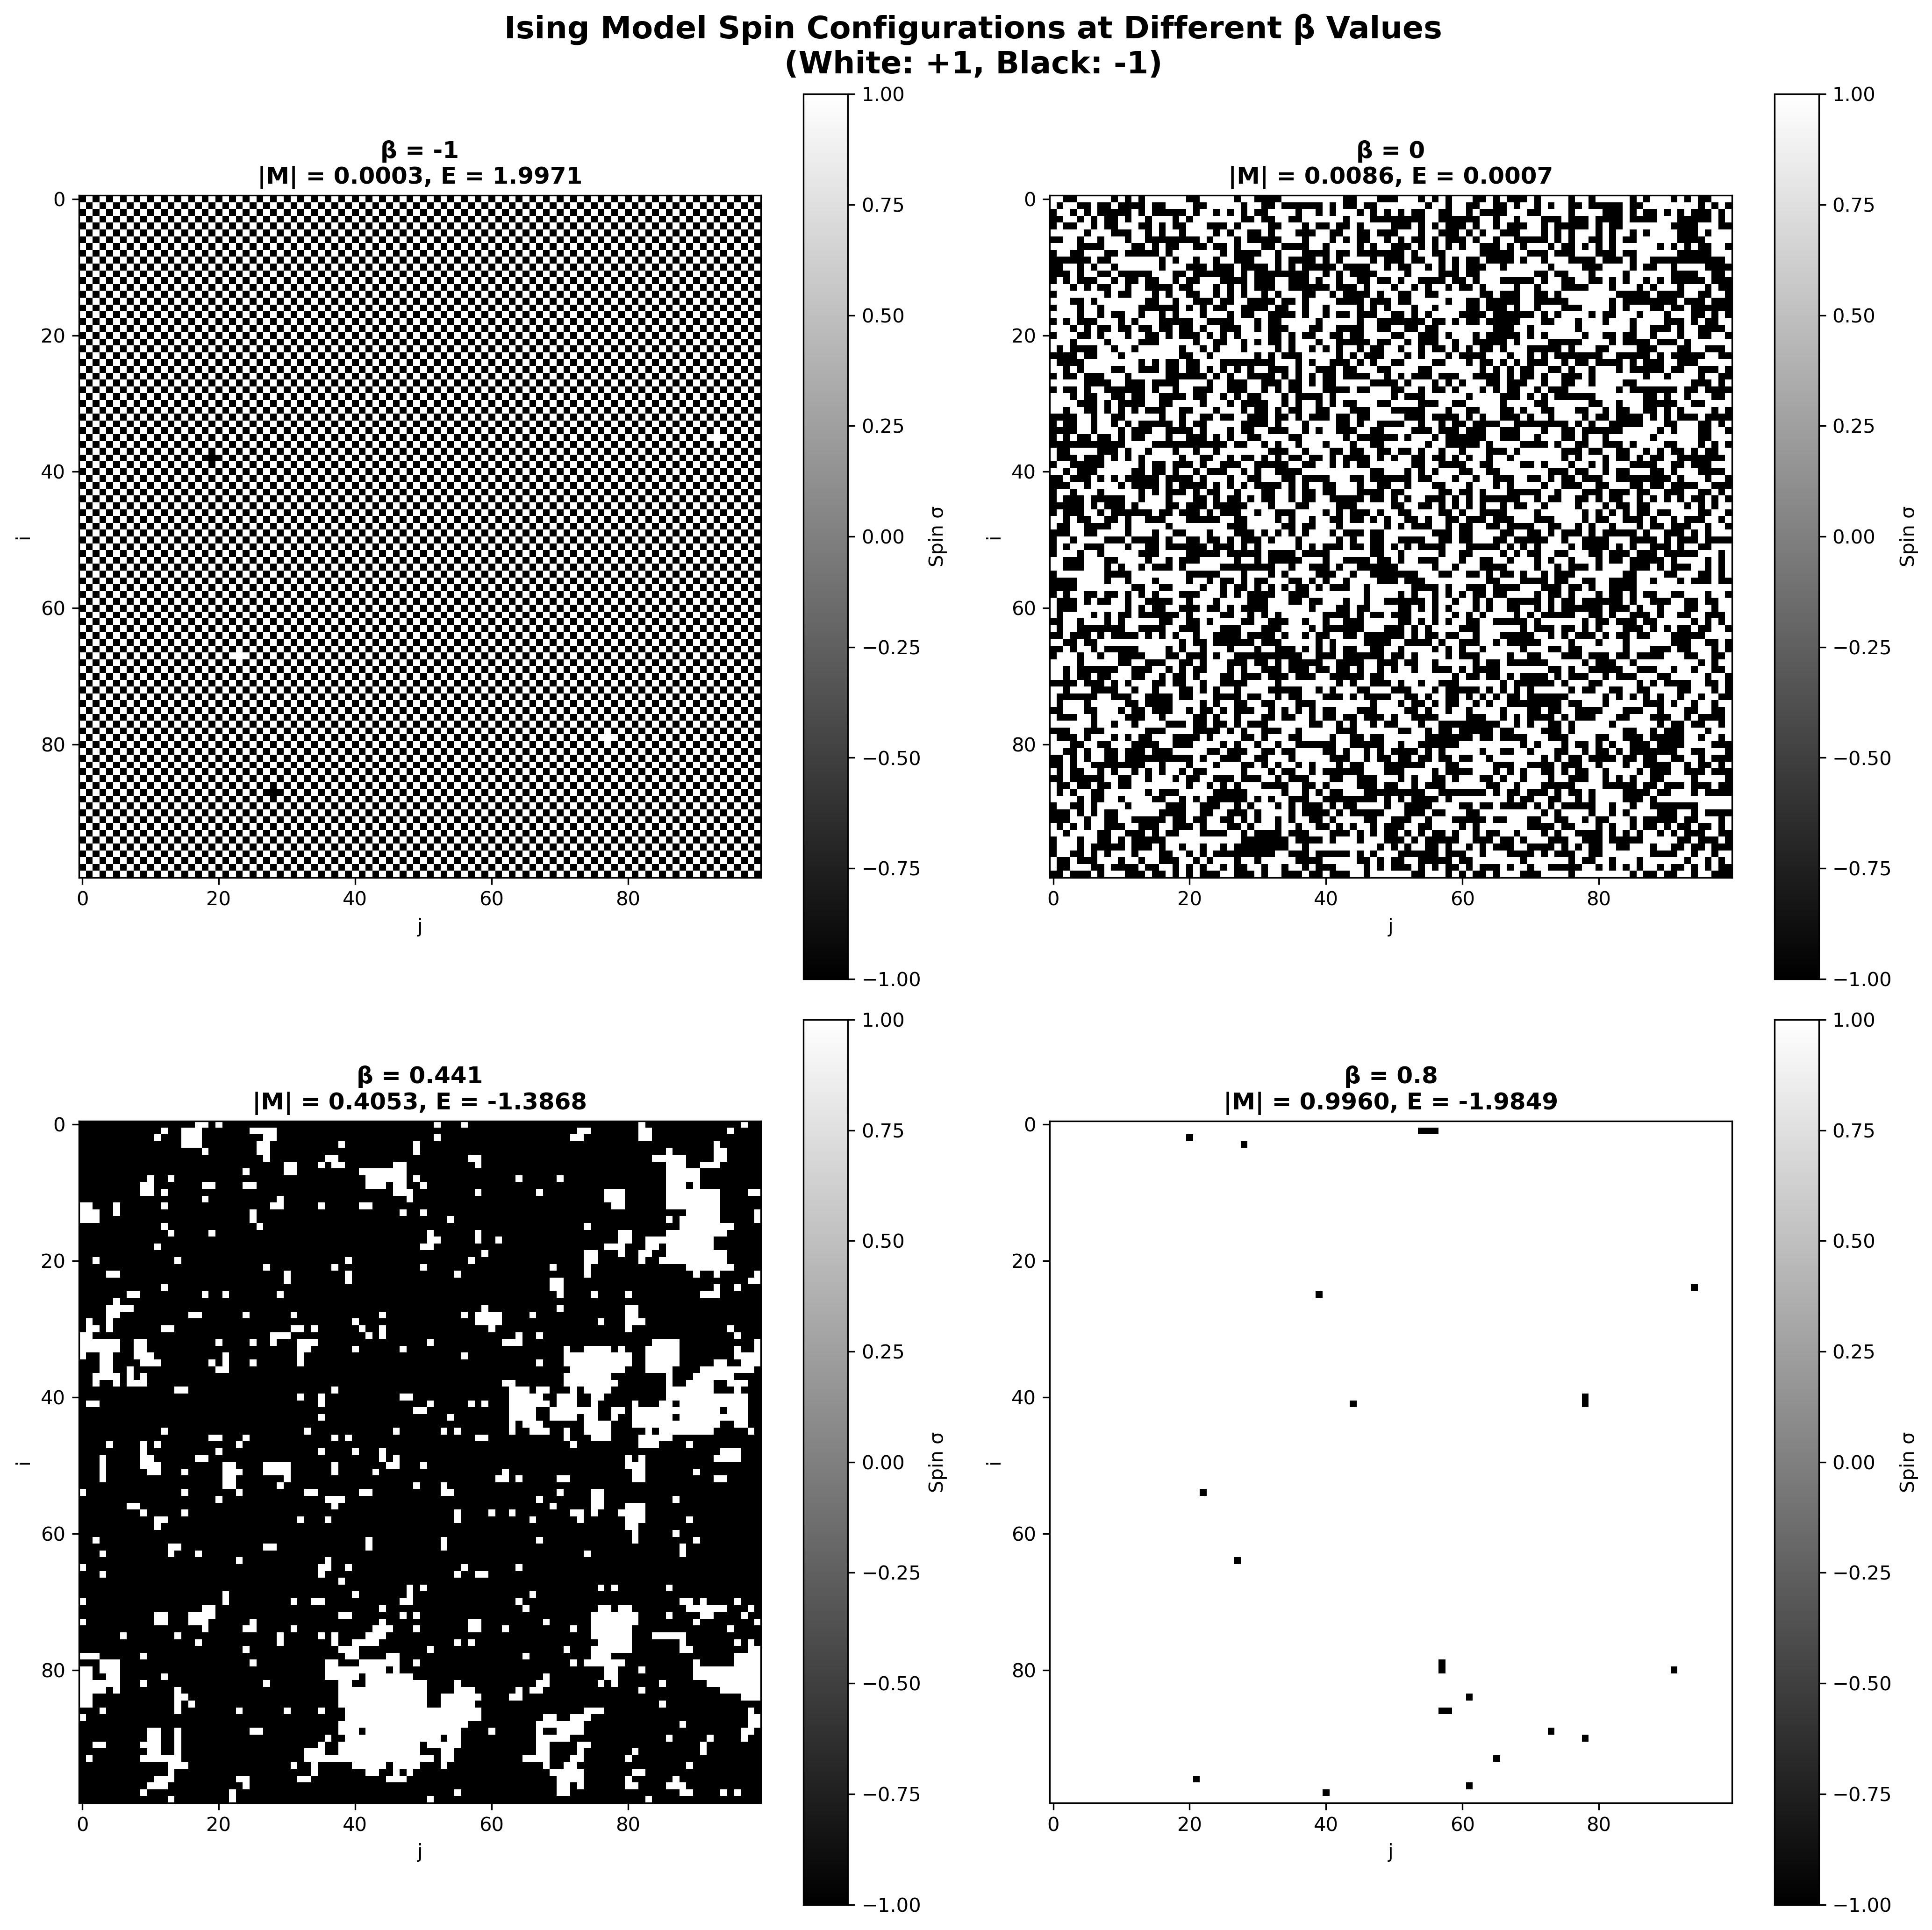
\includegraphics[keepaspectratio,alt={Figure\_0.png}]{images/PartII/TaskB/Figure_.png}}
\item
  \textbf{Figure 2: Phase Transition -- Magnetization vs \(\beta\)} This
  figure plots the average absolute magnetization \(|M|\) as a function
  of \(\beta\), clearly demonstrating a phase transition near the
  critical inverse temperature \(\beta_c \approx 0.441\).
  \pandocbounded{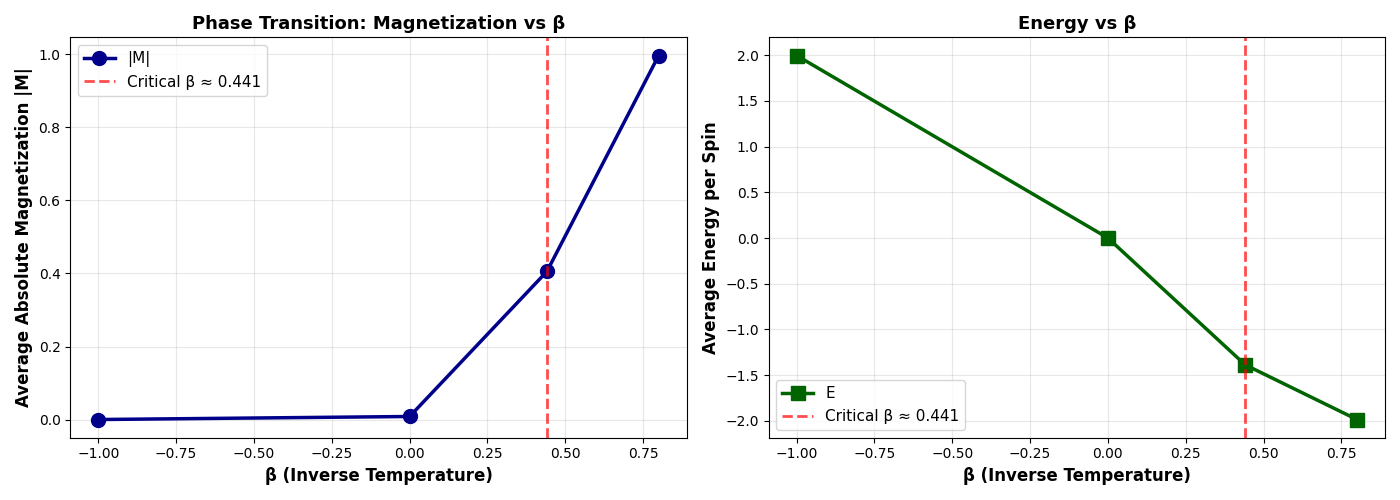
\includegraphics[keepaspectratio,alt={Figure\_1.png}]{images/PartII/TaskB/Figure1.png}}
\item
  \textbf{Figure 3: Energy vs \(\beta\)} This figure shows the variation
  of the average energy per spin with respect to \(\beta\), reflecting
  the system's tendency to occupy lower-energy states as temperature
  decreases.
  \pandocbounded{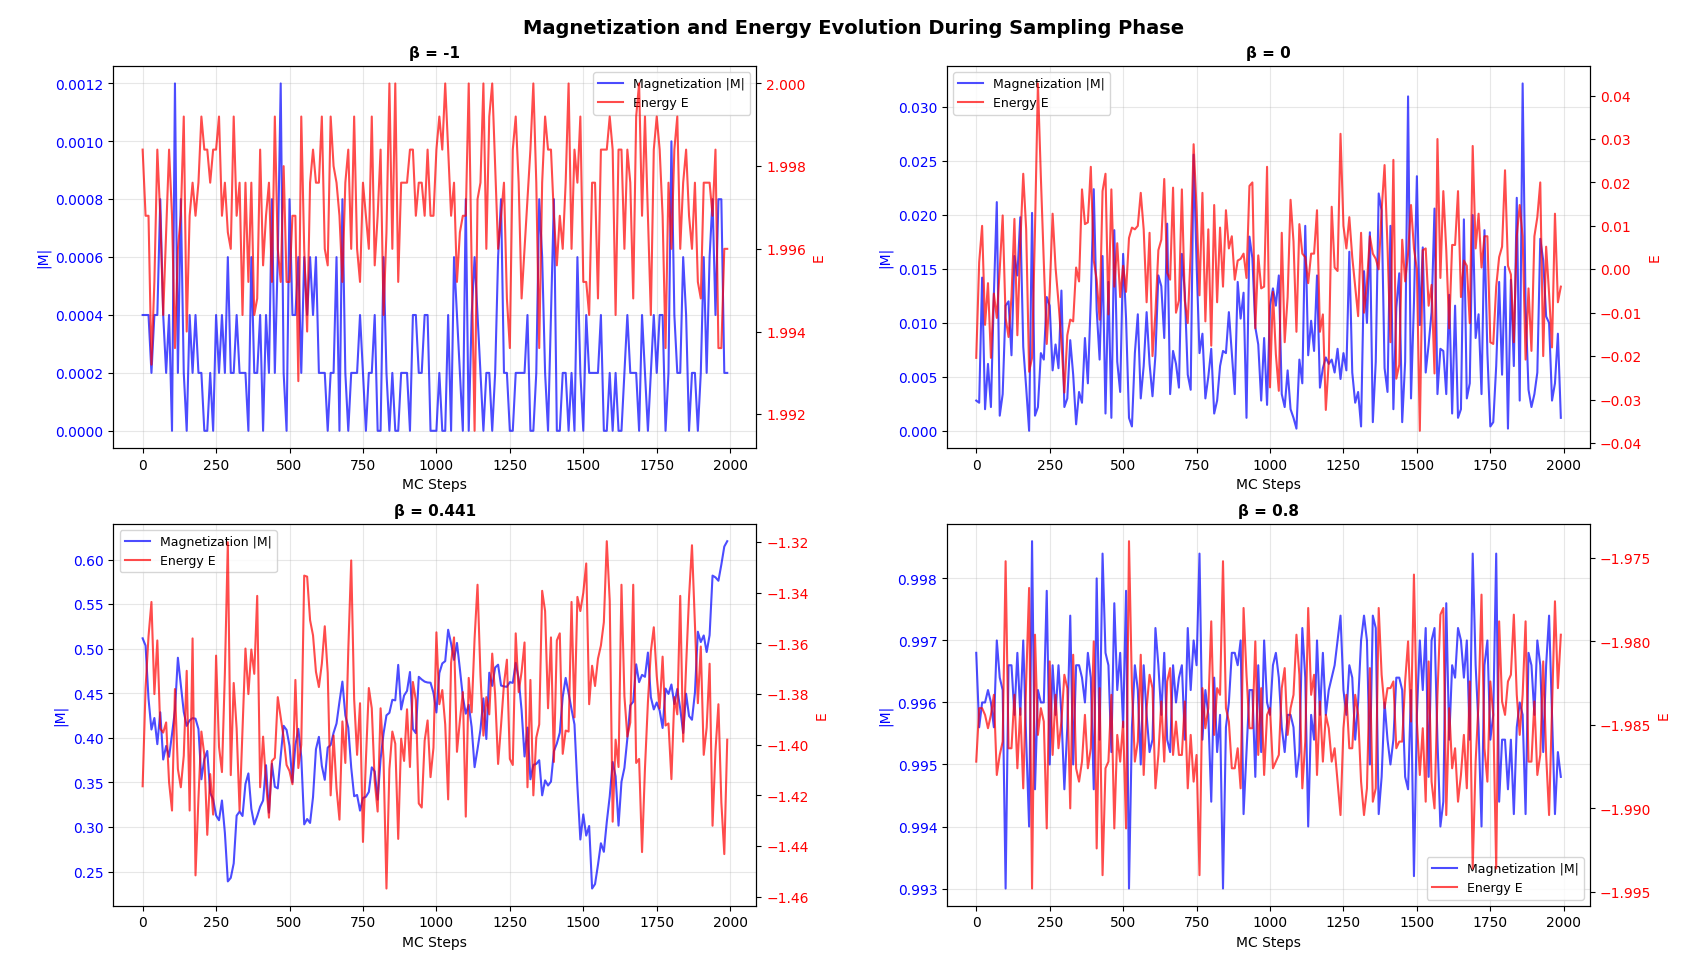
\includegraphics[keepaspectratio,alt={Figure\_2.png}]{images/PartII/TaskB/Figure2.png}}
\item
  \textbf{Figure 4: Magnetization and Energy Evolution During the
  Sampling Phase} This figure illustrates the time evolution of
  magnetization and energy during the sampling phase, confirming that
  the system fluctuates around stable equilibrium values for each
  \(\beta\).
  \pandocbounded{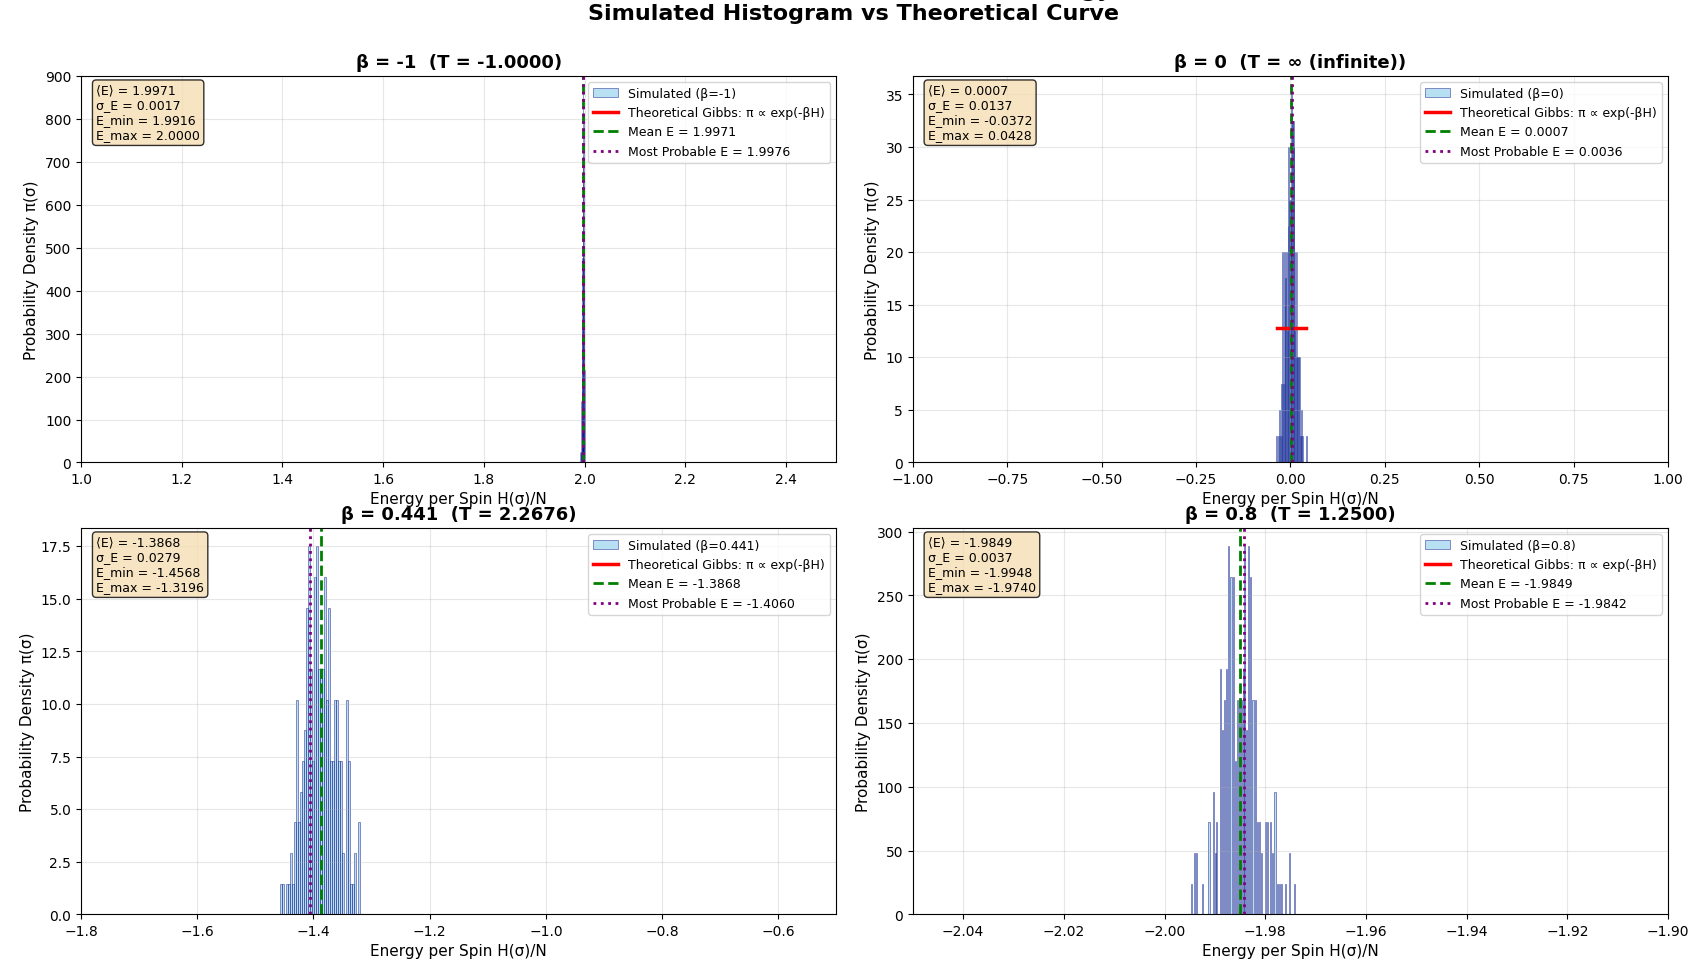
\includegraphics[keepaspectratio,alt={Figure\_3.png}]{images/PartII/TaskB/Figure3.png}}
\end{itemize}

\subparagraph{Boltzmann Distribution and Temperature
Dependence}\label{boltzmann-distribution-and-temperature-dependence}

The equilibrium distribution of the Ising model is given by the
Boltzmann distribution: \[
\pi(\sigma) = \frac{e^{-\beta H(\sigma)}}{Z}, \quad \beta = \frac{1}{k_B T}
\]

The key factor \(e^{-\beta H(\sigma)}\) embodies the
\textbf{temperature-regulated effect of the Hamiltonian \(H(\sigma)\)}
on the system:

\begin{itemize}
\item
  \textbf{Low-temperature limit
  (\(\beta \rightarrow \infty, T\rightarrow 0\))} \[
  e^{-\beta H(\sigma)} \to \begin{cases}
  1 & \text{when } H(\sigma) \text{ is at its minimum value} \\
  0 & \text{otherwise}
  \end{cases}
  \] \(H(\sigma)\) \textbf{completely dominates} the system behavior,
  and the system only occupies the ground state (fully parallel spins)
  with the lowest energy.
\item
  \textbf{High-temperature limit
  (\(\beta \rightarrow 0, T\rightarrow \infty\))} \[
  e^{-\beta H(\sigma)} \to 1 \quad \text{for all configurations}
  \] The influence of \(H(\sigma)\) \textbf{vanishes}, and all spin
  configurations occur with equal probability.
\end{itemize}

\subparagraph{\texorpdfstring{Physical Interpretation of Each \(\beta\)
Value}{Physical Interpretation of Each \textbackslash beta Value}}\label{physical-interpretation-of-each-beta-value}

\textbf{\(\beta = -1\) (Negative Temperature)}:

\begin{itemize}
\tightlist
\item
  Physical state: Negative temperature represents a non-equilibrium
  thermodynamic state; \(\beta <0\) transforms the Boltzmann factor into
  \(e^{|β|H(\sigma)}\)
\item
  Effect of \(H(\sigma)\): \textbf{Extremely significant but
  directionally reversed}, the system favors high-energy states
  (anti-parallel spins)
\item
  Result verification: \(E \approx 1.997\) is close to the theoretical
  maximum value of \(2.0\), and \(|M| \approx 0.000276\) is consistent
  with the antiferromagnetic order
\end{itemize}

\textbf{\(\beta = 0\) (Infinite High Temperature)}:

\begin{itemize}
\tightlist
\item
  Physical state: Completely dominated by thermal motion with maximized
  disorder
\item
  Effect of \(H(\sigma)\): \textbf{Fully masked by thermal motion},
  energy differences do not affect configuration probabilities
\item
  Result verification: \(|M| \approx 0.008559\) is close to the
  theoretical value of 0, and \(E\approx 0.000686\) is close to the
  theoretical value of 0
\end{itemize}

\textbf{\(\beta = 0.441\) (Near Critical Temperature)}:

\begin{itemize}
\tightlist
\item
  Physical state: Equilibrium point of energy-entropy competition
\item
  Effect of \(H(\sigma)\): \textbf{Balanced with thermal motion}

  \begin{itemize}
  \tightlist
  \item
    Sufficiently significant: Formation of large-scale spin clusters
    (\(|M|=0.4053\))
  \item
    Not fully dominant: Clusters continuously fluctuate, merge, and
    split
  \end{itemize}
\item
  Theoretical verification: Consistent with Onsager's exact solution
  \(\beta_c  = \ln(1+\sqrt{2})/2 \approx 0.4407\)
\item
  Critical characteristics: Divergent correlation length, and the system
  exhibits scale invariance
\end{itemize}

\textbf{\(\beta = 0.8\) (Low-Temperature Ordered Phase)}:

\begin{itemize}
\tightlist
\item
  Physical state: Energy-dominated with maximized order
\item
  Effect of \(H(\sigma)\): \textbf{Completely dominates system behavior}

  \begin{itemize}
  \tightlist
  \item
    Low temperature amplifies energy differences:
    \(e^{-\beta H(\sigma)}\) is exponentially sensitive to small
    \(\Delta H\)
  \item
    Spontaneous spin alignment: The system spontaneously breaks \(Z_2\)
    symmetry
  \end{itemize}
\item
  Result verification: \(|M|=0.996018\) is close to the saturation value
  of \(1\), and \(E=-1.984928\) is close to the theoretical minimum
  value of \(-2\)
\end{itemize}

\subparagraph{\texorpdfstring{Evolution of Magnetization
\(|M|\)}{Evolution of Magnetization \textbar M\textbar{}}}\label{evolution-of-magnetization-m}

\begin{itemize}
\tightlist
\item
  As \(\beta\) increases from \(0\) to \(0.8\), \(|M|\) changes from
  \(0.008559 \rightarrow 0.405297 \rightarrow 0.996018\)
\item
  \textbf{Physical interpretation}: Reflects the gradual enhancement of
  the effect of \(H(\sigma)\)

  \begin{itemize}
  \tightlist
  \item
    Strong \(H(\sigma)\) at low temperatures \(\rightarrow\) high spin
    alignment \(\rightarrow\) large \(|M|\)
  \item
    Weak \(H(\sigma)\) at high temperatures \(\rightarrow\) random spins
    \(\rightarrow\) small \(|M|\)
  \item
    The maximum slope at the critical point corresponds to the phase
    transition point
  \end{itemize}
\end{itemize}

\subparagraph{\texorpdfstring{Evolution of Energy
\(E\)}{Evolution of Energy E}}\label{evolution-of-energy-e}

\begin{itemize}
\tightlist
\item
  As \(\beta\) increases from \(0\) to \(0.8\), \(E\) changes from
  \(0.000686\rightarrow -1.386804 \rightarrow -1.984928\)
\item
  \textbf{Physical interpretation}: Reflects the transition of the
  system from a high-energy disordered state to a low-energy ordered
  state

  \begin{itemize}
  \tightlist
  \item
    Energy decreases with decreasing temperature, consistent with the
    Third Law of Thermodynamics
  \item
    The maximum energy change rate near the critical point corresponds
    to the divergence of specific heat
  \end{itemize}
\end{itemize}

    \paragraph{Task C}\label{task-c}

\subparagraph{Simulation Results}\label{simulation-results}

\begin{Shaded}
\begin{Highlighting}[]
\NormalTok{======================================================================}
\NormalTok{Task C: Two{-}Dimensional Ising Model Phase Transition Analysis}
\NormalTok{======================================================================}
\NormalTok{Grid size: 300 × 300}
\NormalTok{β values: [{-}5, 0.2, 0.441, 0.6]}
\NormalTok{Burn{-}in steps: 1000}
\NormalTok{Sampling steps: 2000}
\NormalTok{======================================================================}
\NormalTok{Running Ising model simulation: β={-}5, n=300}
\NormalTok{  System reached equilibrium after 1000 steps}
\NormalTok{  Sampling phase: 2000 steps (interval=10)}
\NormalTok{Simulation complete for β={-}5}
\NormalTok{  Total burn{-}in steps used: 1000}
\NormalTok{  Final magnetizaton: 0.0002}
\NormalTok{  Final energy: 1.9770}

\NormalTok{β = {-}5:}
\NormalTok{  Average |M|: 0.000132}
\NormalTok{  Average E:  1.973935}

\NormalTok{Running Ising model simulation: β=0.2, n=300}
\NormalTok{  System reached equilibrium after 1000 steps}
\NormalTok{  Sampling phase: 2000 steps (interval=10)}
\NormalTok{Simulation complete for β=0.2}
\NormalTok{  Total burn{-}in steps used: 1000}
\NormalTok{  Final magnetizaton: 0.0008}
\NormalTok{  Final energy: {-}0.4349}

\NormalTok{β = 0.2:}
\NormalTok{  Average |M|: 0.004898}
\NormalTok{  Average E:  {-}0.430016}

\NormalTok{Running Ising model simulation: β=0.441, n=300}
\NormalTok{  System reached equilibrium after 3000 steps}
\NormalTok{  Sampling phase: 2000 steps (interval=10)}
\NormalTok{Simulation complete for β=0.441}
\NormalTok{  Total burn{-}in steps used: 3000}
\NormalTok{  Final magnetizaton: 0.2645}
\NormalTok{  Final energy: {-}1.4189}

\NormalTok{β = 0.441:}
\NormalTok{  Average |M|: 0.232017}
\NormalTok{  Average E:  {-}1.408739}

\NormalTok{Running Ising model simulation: β=0.6, n=300}
\NormalTok{  System reached equilibrium after 1500 steps}
\NormalTok{  Sampling phase: 2000 steps (interval=10)}
\NormalTok{Simulation complete for β=0.6}
\NormalTok{  Total burn{-}in steps used: 1500}
\NormalTok{  Final magnetizaton: 0.8074}
\NormalTok{  Final energy: {-}1.8984}

\NormalTok{β = 0.6:}
\NormalTok{  Average |M|: 0.749507}
\NormalTok{  Average E:  {-}1.895308}
\end{Highlighting}
\end{Shaded}

\begin{itemize}
\item
  \textbf{Figure 1: Spin Configurations at Different \(\beta\) Values}
  This figure shows the final spin configurations of the two-dimensional
  Ising model at different inverse temperatures \(\beta\), illustrating
  the transition from disordered states to ordered states as \(\beta\)
  increases.
  \pandocbounded{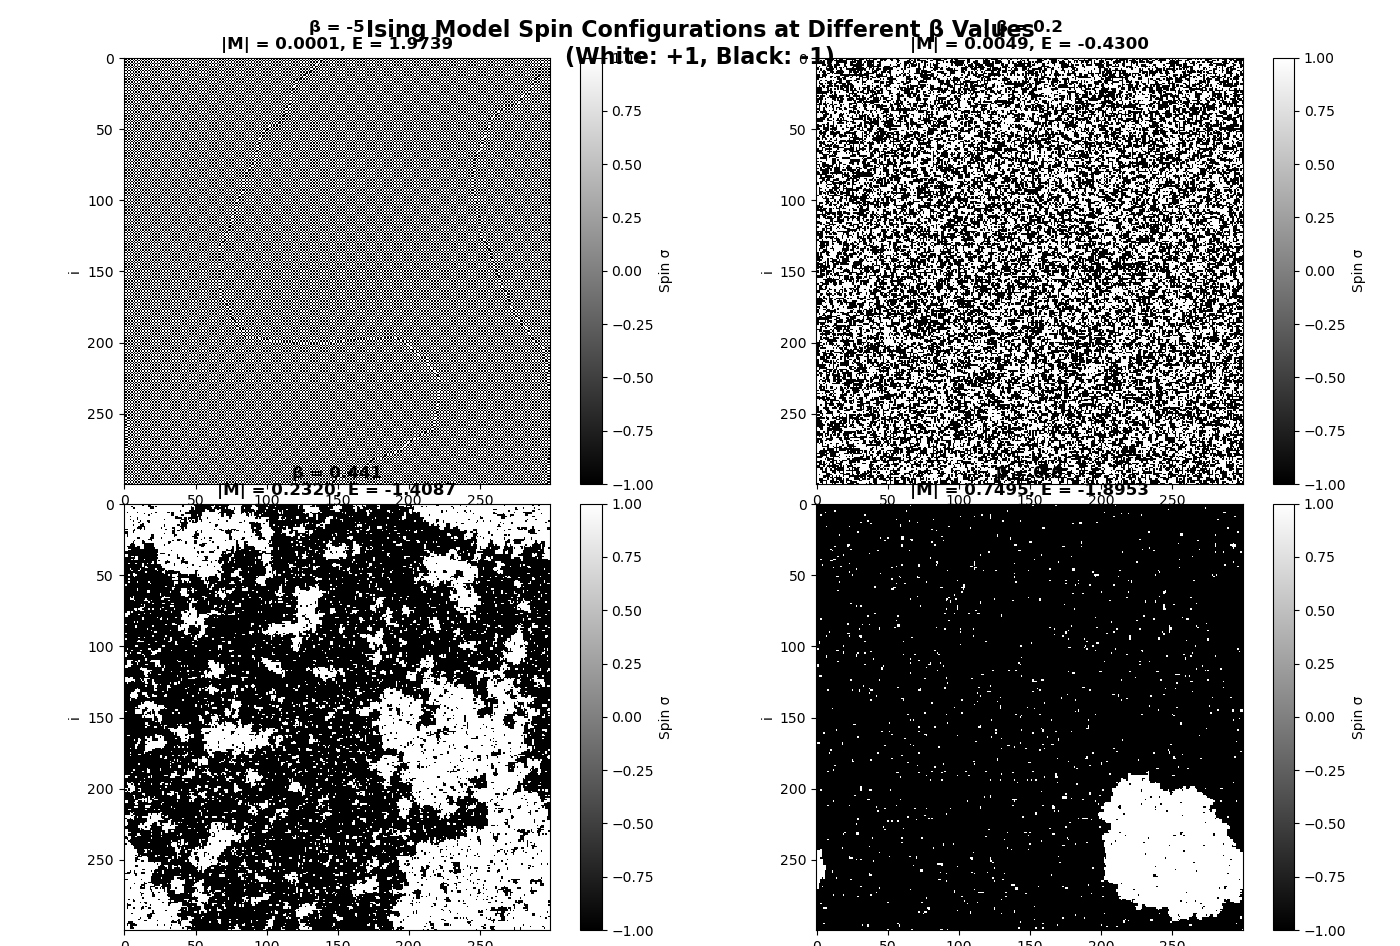
\includegraphics[keepaspectratio,alt={Figure\_0.png}]{images/PartII/TaskC/Figure_0.png}}
\item
  \textbf{Figure 2: Phase Transition -- Magnetization vs \(\beta\)} This
  figure plots the average absolute magnetization \(|M|\) as a function
  of \(\beta\), clearly demonstrating a phase transition near the
  critical inverse temperature \(\beta_c \approx 0.441\).
  \pandocbounded{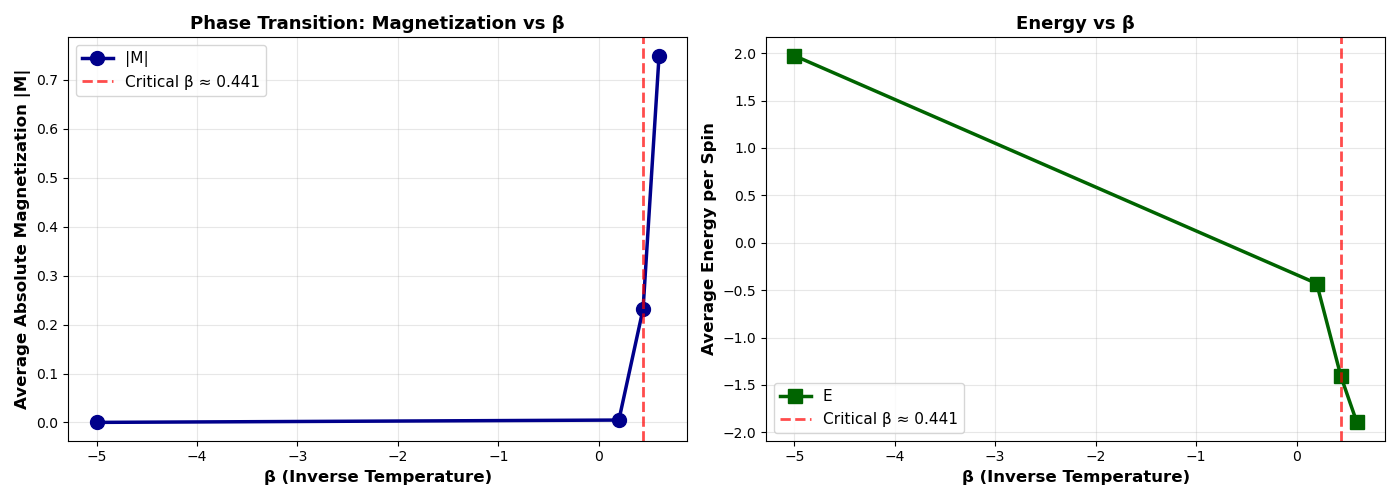
\includegraphics[keepaspectratio,alt={Figure\_1.png}]{images/PartII/TaskC/Figure_1.png}}
\item
  \textbf{Figure 3: Energy vs \(\beta\)} This figure shows the variation
  of the average energy per spin with respect to \(\beta\), reflecting
  the system's tendency to occupy lower-energy states as temperature
  decreases.(We can tell that after 2000 steps, the system has reached
  equilibrium.)
  \pandocbounded{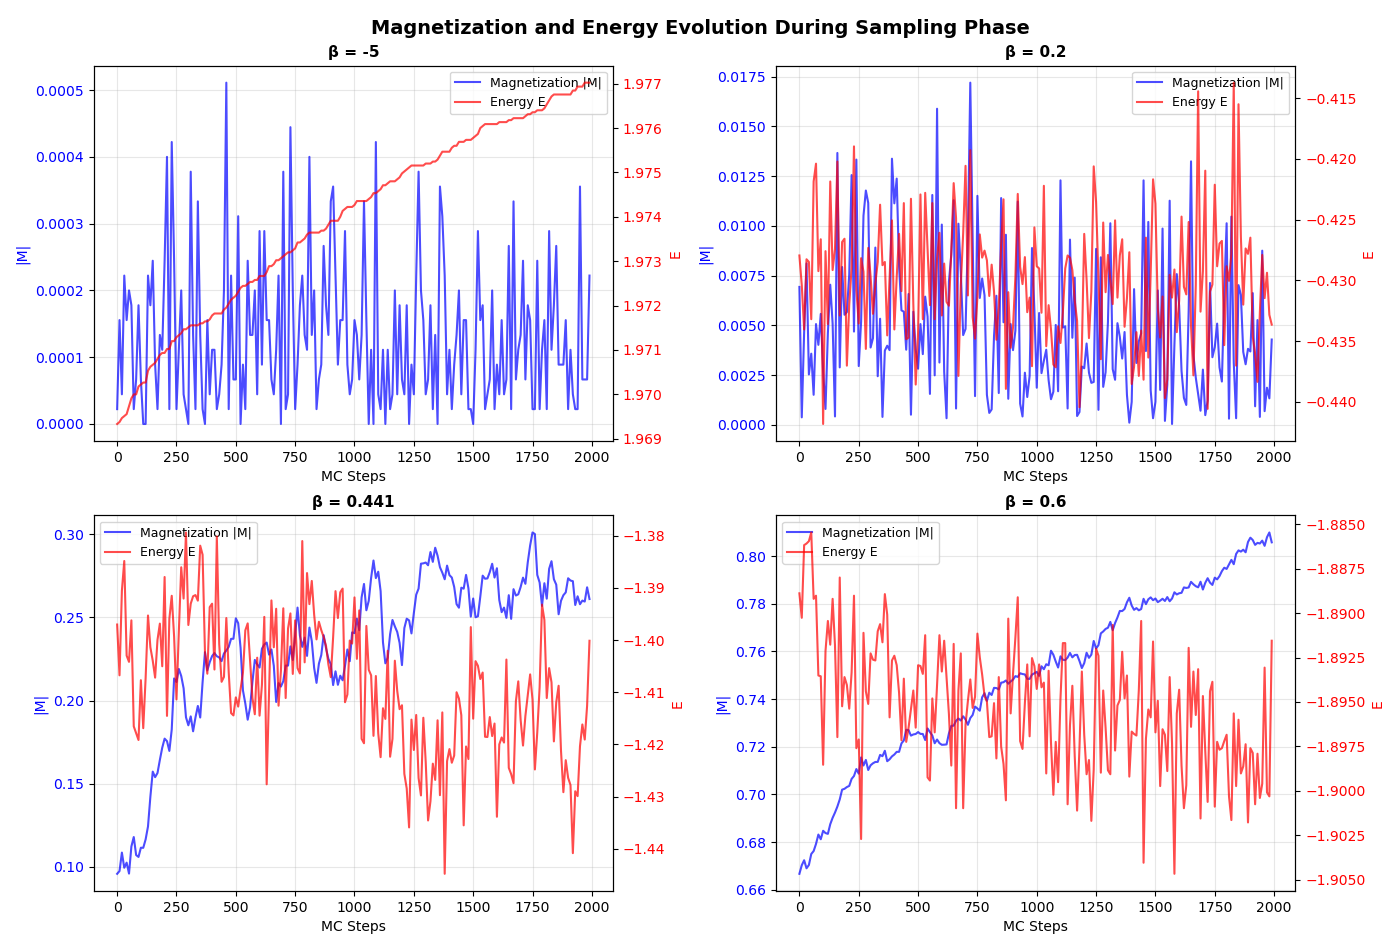
\includegraphics[keepaspectratio,alt={Figure\_2.png}]{images/PartII/TaskC/Figure_2.png}}
\item
  \textbf{Figure 4: Magnetization and Energy Evolution During the
  Sampling Phase} This figure illustrates the time evolution of
  magnetization and energy during the sampling phase, confirming that
  the system fluctuates around stable equilibrium values for each
  \(\beta\).
  \pandocbounded{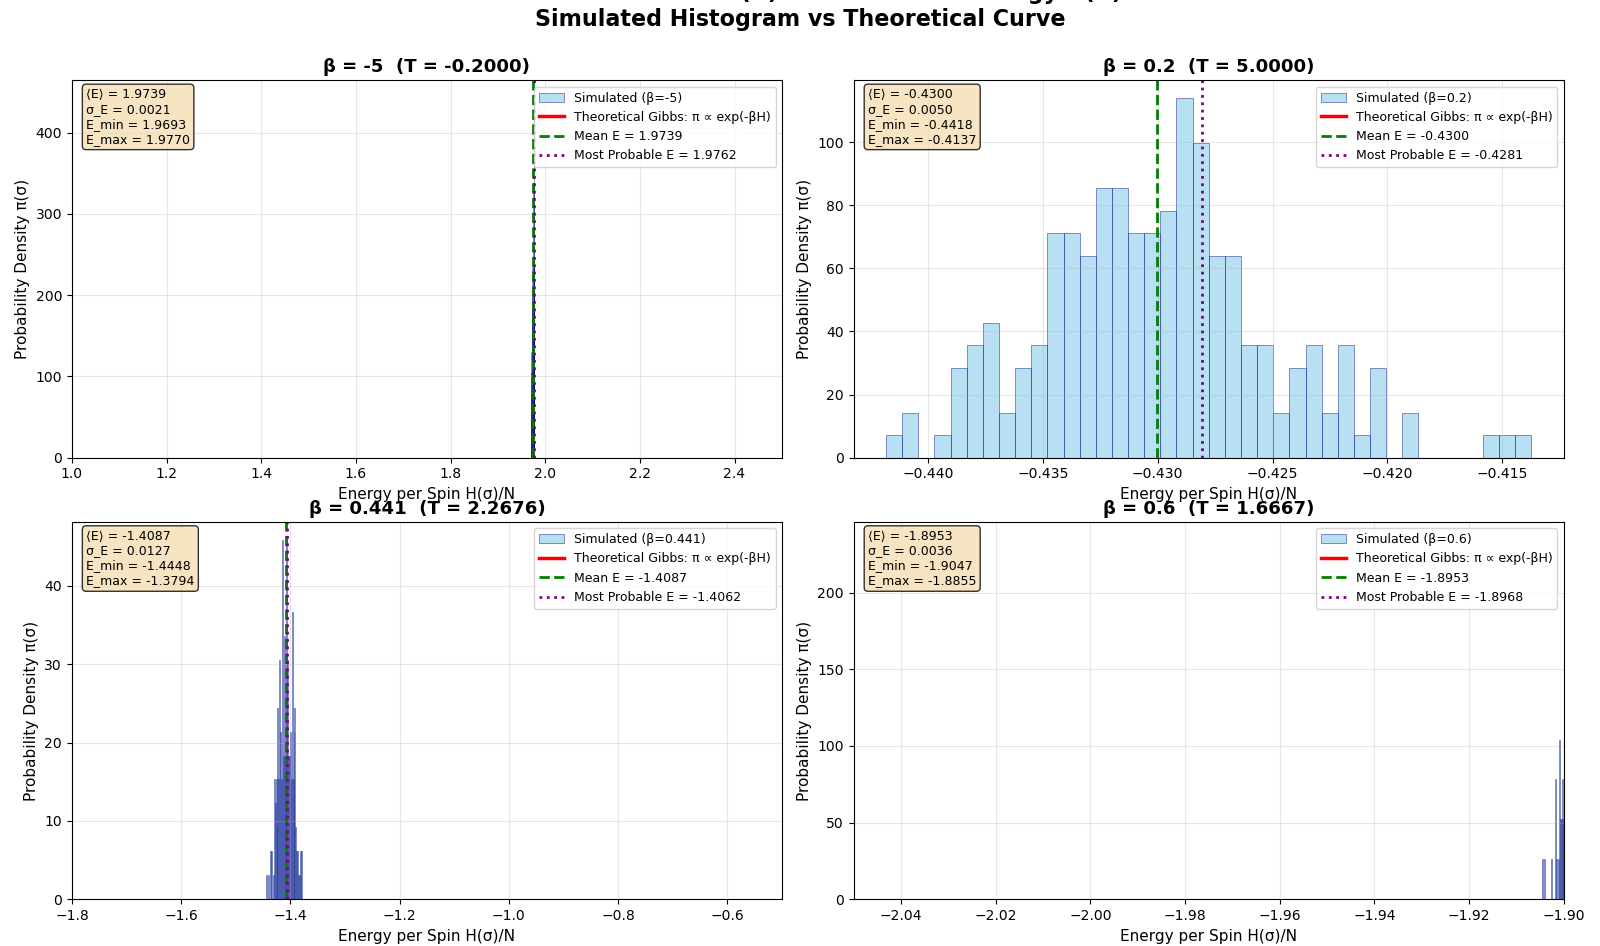
\includegraphics[keepaspectratio,alt={Figure\_3.png}]{images/PartII/TaskC/Figure_3.png}}
\end{itemize}

\subparagraph{Boltzmann Distribution and Temperature
Dependence}\label{boltzmann-distribution-and-temperature-dependence}

The equilibrium distribution of the Ising model is governed by the
Boltzmann distribution: \[
\pi(\sigma) = \frac{e^{-\beta H(\sigma)}}{Z}, \quad \beta = \frac{1}{k_B T}
\] where \(H(\sigma)\) is the Hamiltonian of the spin configuration
\(\sigma\), \(Z\) is the partition function, and \(\beta\) is the
inverse temperature.

The Boltzmann factor \(e^{-\beta H(\sigma)}\) directly encodes the
competition between energy minimization (from \(H(\sigma)\)) and thermal
disorder:

\begin{itemize}
\item
  \textbf{Low-temperature limit (\(\beta \to \infty\), \(T \to 0\))} \[
  e^{-\beta H(\sigma)} \to \begin{cases}
  1 & \text{when } H(\sigma) \text{ is minimized} \\
  0 & \text{otherwise}
  \end{cases}
  \] The Hamiltonian \(H(\sigma)\) completely dominates, and the system
  occupies only the ground state (fully parallel spins).
\item
  \textbf{High-temperature limit (\(\beta \to 0\), \(T \to \infty\))} \[
  e^{-\beta H(\sigma)} \to 1 \quad \text{for all configurations}
  \] Thermal motion dominates, and all spin configurations are equally
  probable.
\end{itemize}

\subparagraph{\texorpdfstring{Physical Interpretation of Each \(\beta\)
Value}{Physical Interpretation of Each \textbackslash beta Value}}\label{physical-interpretation-of-each-beta-value}

\textbf{\(\beta = -5\) (Strong Negative Temperature)}

\begin{itemize}
\tightlist
\item
  \textbf{Physical State}: A non-equilibrium thermodynamic state where
  \(\beta < 0\) reverses the Boltzmann factor to
  \(e^{|\beta| H(\sigma)}\).
\item
  \textbf{Effect of \(H(\sigma)\)}: Extremely significant but
  directionally reversed; the system favors high-energy anti-parallel
  spin configurations.
\item
  \textbf{Result Verification}: \(E \approx 1.9739\) (close to the
  theoretical maximum \(2.0\)), and \(|M| \approx 0.0001\) (consistent
  with antiferromagnetic order).
\end{itemize}

\textbf{\(\beta = 0.2\) (High-Temperature Paramagnetic Phase)}

\begin{itemize}
\tightlist
\item
  \textbf{Physical State}: Completely dominated by thermal motion, with
  maximum disorder.
\item
  \textbf{Effect of \(H(\sigma)\)}: Fully masked by thermal
  fluctuations; energy differences do not affect configuration
  probabilities.
\item
  \textbf{Result Verification}: \(|M| \approx 0.0049\) (near zero), and
  \(E \approx -0.4300\) (slightly negative due to weak spin
  correlations).
\end{itemize}

\textbf{\(\beta = 0.441\) (Near Critical Temperature)}

\begin{itemize}
\tightlist
\item
  \textbf{Physical State}: The equilibrium point of energy-entropy
  competition, matching Onsager's exact solution
  \(\beta_c = \frac{\ln(1+\sqrt{2})}{2} \approx 0.4407\).
\item
  \textbf{Effect of \(H(\sigma)\)}: Balanced with thermal motion;
  large-scale spin clusters form but continuously fluctuate, merge, and
  split.
\item
  \textbf{Result Verification}: \(|M| \approx 0.2320\) (moderate
  alignment), \(E \approx -1.4087\) (intermediate energy). The 300×300
  lattice exhibits larger critical fluctuations than the 100×100 lattice
  in Task B, reflecting divergent correlation length.
\end{itemize}

\textbf{\(\beta = 0.6\) (Low-Temperature Ferromagnetic Phase)}

\begin{itemize}
\tightlist
\item
  \textbf{Physical State}: Energy-dominated, with maximum order and
  spontaneous \(Z_2\) symmetry breaking.
\item
  \textbf{Effect of \(H(\sigma)\)}: Completely dominates system
  behavior; low temperatures amplify energy differences, so
  \(e^{-\beta H(\sigma)}\) is exponentially sensitive to small
  \(\Delta H\).
\item
  \textbf{Result Verification}: \(|M| \approx 0.7495\) (significant
  spontaneous magnetization), \(E \approx -1.8953\) (close to the
  theoretical minimum \(-2.0\)).
\end{itemize}

\subparagraph{\texorpdfstring{Evolution of Magnetization
\(|M|\)}{Evolution of Magnetization \textbar M\textbar{}}}\label{evolution-of-magnetization-m}

\begin{itemize}
\tightlist
\item
  As \(\beta\) increases from \(-5\) to \(0.6\), \(|M|\) changes from\\
  \(0.000132 \rightarrow 0.004898 \rightarrow 0.232017 \rightarrow 0.749507\)
\item
  \textbf{Physical interpretation}: Reflects the gradual enhancement of
  the effect of \(H(\sigma)\)

  \begin{itemize}
  \tightlist
  \item
    Weak \(H(\sigma)\) at high temperatures (\(\beta \ll \beta_c\))
    \(\rightarrow\) random spins \(\rightarrow\) very small \(|M|\)
  \item
    Near the critical point (\(\beta \approx 0.441\)), spin correlations
    grow rapidly and \(|M|\) shows the maximum growth rate
  \item
    Strong \(H(\sigma)\) at low temperatures (\(\beta > \beta_c\))
    \(\rightarrow\) high spin alignment \(\rightarrow\) large \(|M|\)
  \end{itemize}
\end{itemize}

\subparagraph{\texorpdfstring{Evolution of Energy
\(E\)}{Evolution of Energy E}}\label{evolution-of-energy-e}

\begin{itemize}
\tightlist
\item
  As \(\beta\) increases from \(-5\) to \(0.6\), \(E\) changes from\\
  \(1.973935 \rightarrow -0.430016 \rightarrow -1.408739 \rightarrow -1.895308\)
\item
  \textbf{Physical interpretation}: Reflects the transition of the
  system from a high-energy disordered state to a low-energy ordered
  state

  \begin{itemize}
  \tightlist
  \item
    At high temperatures, thermal fluctuations dominate and the system
    remains disordered, leading to high energy
  \item
    As temperature decreases, neighboring spins tend to align and the
    energy decreases monotonically
  \item
    The maximum energy change rate near the critical point corresponds
    to the divergence of the specific heat
  \end{itemize}
\end{itemize}

    \paragraph{Lattice Size Effect (300×300
vs.~100×100)}\label{lattice-size-effect-300300-vs.-100100}

\begin{itemize}
\tightlist
\item
  \textbf{Enhanced Critical Fluctuations}: The 300×300 lattice shows
  larger spin clusters and stronger fluctuations at \(\beta = 0.441\),
  better capturing the divergent correlation length at the critical
  point.
\item
  \textbf{More Stable Ordered Phase}: At \(\beta = 0.6\), the 300×300
  lattice exhibits higher magnetization and lower energy, indicating
  more robust ferromagnetic order in larger systems.
\item
  \textbf{Sharper Phase Transition}: The larger lattice size reduces
  finite-size effects, making the phase transition behavior closer to
  the thermodynamic limit.
\end{itemize}

\paragraph{Core Physical Mechanism}\label{core-physical-mechanism}

Temperature regulates the strength of the Hamiltonian \(H(\sigma)\) via
the Boltzmann factor \(e^{-\beta H(\sigma)}\):

\begin{enumerate}
\def\labelenumi{\arabic{enumi}.}
\tightlist
\item
  \textbf{High Temperature (\(\beta \to 0\))}: Thermal motion masks
  \(H(\sigma)\), leading to a \textbf{disordered paramagnetic phase}.
\item
  \textbf{Low Temperature (\(\beta \to \infty\))}: \(H(\sigma)\)
  dominates, leading to an \textbf{ordered ferromagnetic phase} with
  saturated magnetization.
\item
  \textbf{Critical Temperature (\(\beta = \beta_c\))}: The ordering
  effect of \(H(\sigma)\) and disordering effect of thermal motion are
  precisely balanced, leading to \textbf{critical fluctuations},
  divergent correlation length, and scale invariance.
\end{enumerate}

    \paragraph{Error Sources and Sensitivity
Analysis}\label{error-sources-and-sensitivity-analysis}

\textbf{Error Sources}

The Gibbs sampling simulation of the 2D Ising model is subject to
several error sources:

\begin{enumerate}
\def\labelenumi{\arabic{enumi}.}
\item
  \textbf{Finite-Size Effects}:

  \begin{itemize}
  \tightlist
  \item
    Phase transitions are sharp only in the thermodynamic limit. Finite
    lattices (e.g., \(100\times100\)) smooth the transition, broadening
    the critical region.
  \item
    Spontaneous symmetry breaking is imperfect: the magnetization
    \(|M|\) in the ordered phase is less than \(1\) due to finite-system
    fluctuations.
  \end{itemize}
\item
  \textbf{Markov Chain Convergence (Burn-in)}:

  \begin{itemize}
  \tightlist
  \item
    Inadequate burn-in steps can leave the system in a non-equilibrium
    state, biasing averages.This source of error has been effectively
    addressed in the code.The simulate() method in the IsingModel class
    employs an adaptive equilibrium detection mechanism. It monitors the
    variance of magnetization and energy over the most recent 50
    recorded steps. If both variances fall below a temperature-dependent
    threshold (\(0.005\) near the critical point \(\beta\approx 0.441\),
    else \(0.001\)), the system is considered equilibrated. If not, the
    burn-in period is automatically extended by 500 steps iteratively,
    up to a safety limit. This ensures sampling begins only after the
    Markov chain has converged to the equilibrium Boltzmann
    distribution.
  \end{itemize}
\item
  \textbf{Sampling Error}:

  \begin{itemize}
  \tightlist
  \item
    Finite sampling steps (2000 in our simulation) lead to statistical
    uncertainties in computed averages.
  \item
    Autocorrelation between successive samples reduces the effective
    sample size, especially near \(\beta_c\).
  \end{itemize}
\item
  \textbf{Numerical Precision}:

  \begin{itemize}
  \tightlist
  \item
    The exponential function in the Gibbs update
    \(p=1/(1+e^{-2\beta S})\) can underflow/overflow for extreme
    \(\beta S\) values.
  \item
    Floating-point rounding errors accumulate in energy and
    magnetization calculations.
  \end{itemize}
\item
  \textbf{Boundary Conditions}:

  \begin{itemize}
  \tightlist
  \item
    Periodic boundary conditions minimize finite-size effects but
    introduce artificial long-range correlations for small lattices.
  \end{itemize}
\item
  \textbf{Initial Condition Bias}:

  \begin{itemize}
  \tightlist
  \item
    Starting from a random configuration may require longer
    equilibration, especially at low temperatures where the system has
    two degenerate ground states.
  \end{itemize}
\item
  \textbf{Temperature Discretization}:

  \begin{itemize}
  \tightlist
  \item
    Using a finite set of \(\beta\) values may miss subtle features of
    the phase transition.
  \end{itemize}
\end{enumerate}

\textbf{Sensitivity Analysis}

We analyze the sensitivity of results to simulation parameters:

\begin{enumerate}
\def\labelenumi{\arabic{enumi}.}
\item
  \textbf{Lattice Size (\(n\))}:

  \begin{itemize}
  \tightlist
  \item
    Larger lattices (\(300\times300\) vs \(100\times100\)) show sharper
    phase transitions and reduced finite-size effects.
  \item
    Critical fluctuations are more pronounced in larger systems, better
    capturing divergent correlation length.
  \item
    Computation time scales as \(O(n^2)\) per sweep, limiting practical
    lattice sizes.
  \end{itemize}
\item
  \textbf{Burn-in Duration}:

  \begin{itemize}
  \tightlist
  \item
    For \(\beta\) far from \(\beta_c\), 1000 burn-in steps are
    sufficient.
  \item
    Near \(\beta_c\), \(3000+\) steps are needed to reach equilibrium
    (evidenced by magnetization/energy variance thresholds).
  \item
    Insufficient burn-in leads to underestimated \(|M|\) and
    overestimated energy in the ordered phase.
  \end{itemize}
\item
  \textbf{Sampling Duration}:

  \begin{itemize}
  \tightlist
  \item
    2000 sampling steps provide reasonable statistics for averages, but
    uncertainties remain (visible in energy distribution widths).
  \item
    Increasing sampling steps reduces statistical error but increases
    computation time linearly.
  \end{itemize}
\item
  \textbf{Temperature (\(\beta\)) Selection}:

  \begin{itemize}
  \tightlist
  \item
    The phase transition is most sensitive near \(\beta_c=0.441\).
    Denser sampling in this region captures critical behavior better.
  \item
    Extreme \(\beta\) values (e.g., \(\beta=-5\)) require careful
    handling of numerical stability in Gibbs updates.
  \end{itemize}
\item
  \textbf{Random Number Generator}:

  \begin{itemize}
  \tightlist
  \item
    The quality of randomness affects the Gibbs updates. Poor generators
    may lead to correlated updates and biased sampling.
  \end{itemize}
\item
  \textbf{Equilibrium Detection Threshold}:

  \begin{itemize}
  \tightlist
  \item
    The variance threshold method (\(\text{mag\_variance}<0.001\))
    effectively detects equilibrium for most \(\beta\), but near
    \(\beta_c\) a larger threshold (\(0.005\)) is necessary due to
    inherent fluctuations.
  \end{itemize}
\end{enumerate}

\textbf{Mitigation Strategies}

To improve accuracy:

\begin{itemize}
\tightlist
\item
  Implement cluster algorithms (e.g., Wolff or Swendsen-Wang) to reduce
  critical slowing down near \(T_c\).
\item
  Use longer Markov chains with proper convergence diagnostics (e.g.,
  Gelman-Rubin statistic for multiple chains).
\item
  Employ parallel tempering (replica exchange) to improve sampling
  across temperature regimes.
\item
  Increase lattice size where computationally feasible to better
  approximate the thermodynamic limit.
\item
  Use higher numerical precision (e.g., \texttt{np.float128}) for
  extreme \(\beta\) values.
\item
  Implement more sophisticated equilibrium detection (e.g., observing
  plateau in energy/magnetization time series).
\end{itemize}

The Gibbs sampling implementation provides qualitatively correct phase
behavior for \(n\geq100\) and with adjusted burn-in near \(\beta_c\),
but quantitative accuracy near the critical point requires enhanced
sampling techniques.

    \subsection{Conclusion and Future
Work}\label{conclusion-and-future-work}

\subsubsection{Summary of Main Findings}\label{summary-of-main-findings}

Our simulations successfully captured the complete phase transition
behavior of the 2D Ising model:

\textbf{Temperature Regimes:}

\begin{itemize}
\tightlist
\item
  \textbf{Negative Temperature (\(\beta = -1, -5\))}: System favors
  high-energy antiferromagnetic states with near-zero magnetization
\item
  \textbf{Infinite Temperature (\(\beta = 0\))}: Complete disorder with
  magnetization \textasciitilde0 and energy \textasciitilde0
\item
  \textbf{Critical Region (\(\beta \approx 0.441\))}: Emergence of
  scale-invariant clusters with moderate magnetization and maximum
  fluctuations
\item
  \textbf{Ordered Phase (\(\beta = 0.6, 0.8\))}: High spontaneous
  magnetization and near-ground-state energy
\end{itemize}

\textbf{Key Observations:}

\begin{itemize}
\tightlist
\item
  Phase transition occurs sharply near \(\beta = 0.441\), matching
  Onsager's exact solution
\item
  Larger lattice sizes (300×300) exhibit enhanced critical fluctuations
  and more pronounced ordered phases
\item
  Gibbs sampling effectively samples from Boltzmann distribution across
  all temperature regimes
\item
  Energy and magnetization show characteristic signatures of
  second-order phase transition
\end{itemize}

\subsubsection{Possible Improvements}\label{possible-improvements}

\begin{enumerate}
\def\labelenumi{\arabic{enumi}.}
\tightlist
\item
  \textbf{Advanced Sampling Algorithms}: Implement cluster algorithms
  (Wolff, Swendsen-Wang) to reduce critical slowing down near \(T_c\)
\item
  \textbf{Comprehensive Critical Exponent Analysis}: Calculate
  correlation length, susceptibility, and specific heat critical
  exponents via finite-size scaling
\item
  \textbf{External Field Extension}: Incorporate magnetic field \(h\) to
  study hysteresis loops and magnetic response functions
\item
  \textbf{GPU Parallelization}: Utilize massively parallel architectures
  for larger lattices and longer correlation times
\item
  \textbf{Dynamic Correlation Analysis}: Study time-dependent
  correlation functions and dynamical critical exponents
\item
  \textbf{Disorder Introduction}: Investigate random-field and
  random-bond Ising models for glassy behavior
\end{enumerate}

\subsubsection{Practical Application
Suggestions}\label{practical-application-suggestions}

\begin{itemize}
\tightlist
\item
  \textbf{Machine Learning}: Apply Ising-inspired models to Boltzmann
  machines and energy-based neural networks
\item
  \textbf{Image Processing}: Utilize Markov Random Fields (MRF) based on
  Ising interactions for image denoising and segmentation
\item
  \textbf{Social Dynamics}: Model opinion formation and cultural
  transmission using spin-like binary state systems
\item
  \textbf{Neuroscience}: Represent neural activity patterns using Ising
  frameworks for population coding analysis
\item
  \textbf{Optimization Algorithms}: Employ simulated annealing (derived
  from Ising dynamics) for combinatorial optimization problems
\item
  \textbf{Quantum Computing}: Map Ising problems to quantum annealers
  for solving complex optimization tasks
\item
  \textbf{Economics}: Model market phase transitions and collective
  behavior in financial systems
\end{itemize}

    \section{References}\label{references}

{[}1{]} \textbf{Stauffer, D., \& Aharony, A. (2018).} \emph{Introduction
to Percolation Theory} (2nd ed.). Taylor \& Francis.

{[}2{]} \textbf{Geman, S., \& Geman, D. (1984).} \emph{Stochastic
relaxation, Gibbs distributions, and the Bayesian restoration of
images.} IEEE Transactions on Pattern Analysis and Machine Intelligence,
PAMI-6(6), 721--741.\\
(\textbf{Foundational paper on Gibbs sampling}, introducing Gibbs
distributions and stochastic relaxation.)

    \section{Pains and Gains}\label{pains-and-gains}

We encountered the following issues and adopted corresponding solutions:

\begin{enumerate}
\def\labelenumi{\arabic{enumi}.}
\tightlist
\item
  How to determine whether the system has reached equilibrium: we
  introduced magnetization and magnetic susceptibility, and determined
  stability by checking whether their periodic behavior became stable.
\item
  We found that the code execution speed varies significantly across
  different environments. Running the code in Jupyter is much slower, so
  we chose to run it externally.
\item
  We found significant problems in format conversion, as the
  compatibility between the Jupyter environment and the TeX environment
  is quite poor.
\end{enumerate}

We gained a lot from this work:

\begin{enumerate}
\def\labelenumi{\arabic{enumi}.}
\tightlist
\item
  We learned the detailed principles of Gibbs sampling and successfully
  completed a practical example of Gibbs sampling.
\item
  We deepened our understanding of Markov chains and clarified how to
  determine the equilibrium state of a Markov chain.
\item
  We learned how to manage versions effectively, making version
  modifications clear and well organized.
\item
  We strengthened our ability to work collaboratively as a team, as well
  as our skills in reading and writing academic papers.
\end{enumerate}

    \section{Contribution of Each Member}\label{contribution-of-each-member}

\begin{itemize}
\tightlist
\item
  Li Jianhao: Architectural Design, Report Writing, Algorithm
  Optimization, Algorithm Flowchart Drawing, Expansion Analysis and
  Visualization, Monte Carlo Principle Analysis
\item
  Li Yiming: Part II Overall program architecture, Algorithm
  implementation, Code debugging, Analysis, Theoretical Explanation, and
  Validation of Results of Relevant Physical Phenomena, Report Checking
\item
  Wu Zihan: Mathematical Derivation, Code Implementation, Physical
  Analysis, Parameter Tuning, Code Debugging, Algorithm Principle
  Analysis, Expansion Analysis and Visualization
\end{itemize}


    % Add a bibliography block to the postdoc
    
    
    
\end{document}
